\documentclass[english,phd]{diploma}

% Packages
% enhanced support for quotation marks, support for biblatex package
\usepackage[autostyle=true]{csquotes}
\usepackage[
    backend=biber,
    giveninits=true, % abbreviate author's first names in bibliography
    style=numeric,
    alldates=iso,
    maxnames=999,    % for my own publications
    maxbibnames=3,   % for bibliography
    defernumbers=true,
    urldate=short,
    sorting=none,
    seconds=true
]{biblatex}
\usepackage{dcolumn} % numeric column type
%\usepackage{subfig} % subtables and subfigures

\usepackage{subcaption} % subfigure
\captionsetup{compatibility=false}

\newcolumntype{T}{>{\footnotesize}p{6cm}} % Estee table

\usepackage[cpp]{diplomalst}
\usepackage{hyperref}
%\usepackage{todonotes}
\usepackage{amsmath}
% \mathlarger
\usepackage{relsize}
% \mathbb
\usepackage{amssymb}
\usepackage{tikz}
\usetikzlibrary{graphs}
\usetikzlibrary{positioning}
\usetikzlibrary{arrows.meta}
\usetikzlibrary{automata}
\usetikzlibrary{math}
% Source code highlighting
\usepackage[outputdir=../out,newfloat]{minted}
% Multiple footnotes at one place
\usepackage[multiple]{footmisc}
% Autoref with capitalization (need to use Cref)
\usepackage[nameinlink]{cleveref}
% Horizontal margin configuration in description/enumerate/itemize
\usepackage{enumitem}
% SI units (\micro\second, \mebi\byte)
\usepackage{siunitx}
% HQ comparison table
\usepackage{array}
\usepackage{fullpage}
\usepackage{makecell}
\usepackage{fontawesome}
\usepackage{threeparttable}
\usepackage{wasysym}
% Custom list of definitions
\usepackage{tocloft}

% Abbreviations (\gls, \glspl, \acrfull, \acrshort, \acrlong)
\usepackage[
    acronym,        % enable acronyms
    nomain,         % disable main glossary, we only use acronyms
    notranslate,     % enable overriding \acronymname without involving babel
	toc=false,
]{glossaries-extra}

%\glsdisablehyper    % disable hyperlinks
\renewcommand*{\acronymname}{List of Abbreviations}

\usemintedstyle{vs}
\setminted{tabsize=4}
% [escapeinside=||]
% [tabsize=4]
% [fontsize=\small]

% Fix arrow tips
\tikzset{tips=proper}

% Commands
\newcommand{\comment}[1]{}
\newcommand{\workshare}[1]{\emph{#1}}
\newcommand{\footnoteurl}[1]{\footnote{\url{#1}}}
\newcommand{\Autoref}[1]{\Cref{#1}}

% Tools
\newcommand{\estee}{\textsc{Estee}}
\newcommand{\rsds}{\textsc{RSDS}}
\newcommand{\hyperqueue}{\textsc{HyperQueue}}
\newcommand{\autoalloc}{\emph{autoalloc}}
\newcommand{\Autoalloc}{\emph{Autoalloc}}
\newcommand{\hq}{\textsc{HQ}}
\newcommand{\gnuparallel}{\textsc{GNU parallel}}
\newcommand{\hypershell}{\textsc{HyperShell}}
\newcommand{\dask}{\textsc{Dask}}
\newcommand{\ray}{\textsc{Ray}}
\newcommand{\parsl}{\textsc{Parsl}}
\newcommand{\pycompss}{\textsc{PyCOMPSs}}
\newcommand{\pegasus}{\textsc{Pegasus}}
\newcommand{\balsam}{\textsc{Balsam}}
\newcommand{\autosubmit}{\textsc{AutoSubmit}}
\newcommand{\fireworks}{\textsc{FireWorks}}
\newcommand{\merlin}{\textsc{Merlin}}
\newcommand{\snakemake}{\textsc{SnakeMake}}

% Definitions
\newcommand{\listdefname}{List of Definitions}
\newlistof{taskdefinition}{def}{\listdefname}

% Add a new definition (#1 = label, #2 = name)
\newcommand{\makedef}[2]
{\refstepcounter{taskdefinition}%
[\textbf{Definition~\thetaskdefinition{}}]\label{#1}
\addcontentsline{def}{taskdefinition}{\protect
\numberline{\thesection}Definition \thetaskdefinition{} (#2)}\par}
% Move labels to the right of the section in the list
\addtolength{\cfttaskdefinitionnumwidth}{10pt}

% Add vertical margins between chapters
\let\oldchapter=\chapter
\renewcommand{\chapter}{\addtocontents{def}{\protect\addvspace{10pt}}%
\oldchapter}

\newcommand{\defref}[1]{\hyperref[#1]{Definition~\ref*{#1}}}

% Specific definitions
\newcommand{\fntaskres}{Res_t}
\newcommand{\fntaskresfrac}{\fntaskres^{fr}}
\newcommand{\fntaskresvar}{\fntaskres^{var}}
\newcommand{\fnworkerres}{Res_w}
\newcommand{\fnworkerresident}{\fnworkerres^{id}}
\newcommand{\fntaskresassigned}{RA}
\newcommand{\fntaskvarassigned}{RV}
\newcommand{\fnworkertaskassigned}{WX}
\newcommand{\fntaskworkerassigned}{X}
\newcommand{\fntaskstart}{S}
\newcommand{\fntaskfinish}{F}
\newcommand{\fntaskresvarcount}{RC}
\newcommand{\scheduleworker}{S_w}
\newcommand{\scheduleorder}{S_o}
\newcommand{\setresourcekinds}{RK}
\newcommand{\setresourcekindstaskgraph}{RK_t}
\newcommand{\setresourcekindscluster}{RK_w}
\newcommand{\setresourcekindsident}{RK_w^{id}}
\newcommand{\setresourceelements}{RE}
\newcommand{\powerset}[1]{\mathcal{P}(#1)}
\newcommand{\resourcerequirement}[2]{$#1\colon T \times \setresourcekindstaskgraph \rightarrow \mathbb{#2}_{\geq{}0}$}
\newcommand{\timedomain}{\mathbb{R}_{\geq{}0}}
\newcommand{\taskgraphinner}[1]{(T, O, E, #1, \fntaskres)}
\newcommand{\taskgraphexecution}{$E = (G, C, \fntaskworkerassigned)$}

\graphicspath{{./imgs/}}

% TikZ styles
\tikzset{%
    task/.style={circle, draw},
    data/.style={rectangle, draw, rounded corners},
    arrow/.style={draw, thick, {->}}
}

\renewcommand\lstlistlistingname{List of Source Code Listings}

% Metadata
\ThesisAuthor{Ing. Jakub Beránek}

\ThesisSupervisor{Ing. Jan Martinovič, Ph.D.}

\CzechThesisTitle{Ergonomie a efektivita workflow na HPC klastrech}
\EnglishThesisTitle{Ergonomics and efficiency of workflows on HPC clusters}

\SubmissionYear{2024}

\CzechAbstract{Tato práce se zabývá spouštěním grafů úloh na vysoce výkonných systémech (superpočítačích),
se zaměřením na efektivní využití výpočetních zdrojů a poskytnutí ergonomických rozhraní pro návrh
a spouštění grafů úloh. Programování na základě úloh je oblíbeným způsobem pro definici vědeckých soustav
výpočtů, které jsou určeny pro spouštění na distribuovaných systémech. Nicméně spouštění těchto úloh na superpočítačích
přináší unikátní výzvy, například problémy s výkonem způsobené značným rozsahem úloh nebo problematickou interakci úloh
se systémy pro správu alokací na superpočítačích, jako jsou například PBS (Portable Batch System) nebo Slurm. Tato práce
zkoumá, jaké jsou hlavní problémy ovlivňující spouštění úloh v této oblasti a navrhuje různé přístupy,
které by měly pomoci tyto problémy částečně či zcela vyřešit, a to jak v oblasti výkonu, tak i ergonomie vývoje.

Tato práce poskytuje tři hlavní přínosy. Prvním z nich je prostředí pro simulaci spouštění grafů úloh,
které umožňuje jednoduché experimentování a měření různých plánovacích algoritmů. Toto prostředí bylo
použito pro provedení rozsáhlé studie kvality různých plánovačů úloh. Dále práce analyzuje
výkonnostní charakteristiku moderního nástroje pro spouštění úloh \dask{}, a poskytuje alternativní
implementaci \dask{} serveru, která výrazně zvyšuje jeho efektivitu v případech, které vyžadují vysoký výkon.
Hlavním přínosem práce je metoda pro plánování úloh a správu zdrojů, která umožňuje jednoduché spouštění grafů úloh na heterogenních superpočítačích, které zároveň maximalizuje využití dostupných výpočetních zdrojů. Práce také poskytuje referenční implementaci
využívající této metody v rámci nástroje \hyperqueue{}, který je dostupný jako software s otevřeným zdrojovým kódem pod licencí MIT (Massachusetts Institute of Technology) na adrese \url{https://github.com/it4innovations/hyperqueue}.}
\CzechKeywords{distribuované výpočty, výpočetní grafy, heterogenní zdroje, vysoce výkonné počítání}

\EnglishAbstract{This thesis deals with the execution of task graphs on High-performance Computing
(HPC) clusters (supercomputers), with a focus on efficient usage of hardware resources and ergonomic interfaces for
task graph submission. Task-based programming is a popular approach for defining scientific workflows that can be computed on distributed
clusters. However, executing task graphs on supercomputers introduces unique challenges, such as performance
issues caused by the large scale of HPC workflows or cumbersome interactions with HPC allocation
managers like PBS (Portable Batch System) or Slurm. This work examines what are the main challenges
in this area and how do they affect task graph execution, and it proposes various approaches for alleviating
these challenges, both in terms of efficiency and developer ergonomics.

This thesis provides three main contributions. Firstly, it provides a task graph simulation environment
that enables prototyping and benchmarking of various task scheduling algorithms, and performs a comprehensive
study of the performance of various task schedulers using this environment. Secondly, it analyzes the
bottlenecks and overall performance of a state-of-the-art task runtime \dask{} and provides an implementation
of an alternative \dask{} server which significantly improves its performance in HPC use-cases. And
primarily, it introduces a unified meta-scheduling and resource management design for effortless execution of task graphs on heterogeneous HPC clusters that facilitates efficient usage of hardware resources. It also provides a reference implementation of this design within an HPC-tailored task runtime called \hyperqueue{}, which is available as open-source software under the MIT (Massachusetts Institute of Technology) license at \url{https://github.com/it4innovations/hyperqueue}.}
\EnglishKeywords{distributed computing, task graphs, heterogeneous resources, hpc}

\Acknowledgement{I would like to thank my supervisor, Jan Martinovič, for his advice.
I would also like to thank Ada Böhm, Vojtěch Cima and Martin Šurkovský, who have co-authored several
publications with me and supported me during my PhD studies. I am especially grateful to Ada Böhm
for her mentorship and constant readiness to provide both research and technical guidance. I would like
to express my gratitude to all the wonderful people that I met during my internship at the SPCL lab at ETH Zurich.
Furthermore, my thanks also go to Vanessa DeRhen for proofreading this thesis.

\vspace{2mm}The development of \estee{} was supported by several projects.
It has received funding from the European High-Performance Computing Joint Undertaking (JU)
under grant agreement No 955648. This work was supported by the Ministry of Education, Youth and Sports of the Czech Republic the e-INFRA CZ (ID: 90140) and ACROSS (ID: MC2104) projects.

The development of \hyperqueue{} was supported by several projects.
It has received funding from the European High-Performance Computing Joint Undertaking (JU) under grant agreement No 956137.
This work was supported by the Ministry of Education, Youth and Sports of the Czech Republic through the e-INFRA CZ (ID: 90254) and LIGATE (ID: MC2102)
projects.

\vspace{2mm}Last but not least, I thank my wife Jana for her support and endless patience.}

\addbibresource{references.bib}
\addbibresource{publications.bib}

\makeglossaries
\setabbreviationstyle[acronym]{short-long}
\newacronym{abfe}{ABFE}{Absolute Binding Free Energy}
\newacronym{ai}{AI}{Artificial Intelligence}
\newacronym{api}{API}{Application Programming Interface}
\newacronym{arcce}{ARC-CE}{Advanced Resource Connector Compute Element}
\newacronym{awh}{AWH}{Accelerated Weight Histogram}
\newacronym{cadd}{CADD}{Computer-aided Drug Design}
\newacronym{ci}{CI}{Continuous Integration}
\newacronym{cli}{CLI}{Command-line Interface}
\newacronym{cpu}{CPU}{Central Processing Unit}
\newacronym{csv}{CSV}{Comma-separated Values}
\newacronym{dag}{DAG}{Directed Acyclic Graph}
\newacronym{dsl}{DSL}{Domain-specific Language}
\newacronym{fpga}{FPGA}{Field-programmable Gate Array}
\newacronym{gcc}{GCC}{GNU Compiler Collection}
\newacronym{gil}{GIL}{Global Interpreter Lock}
\newacronym{gpfs}{GPFS}{General Parallel File System}
\newacronym{gpu}{GPU}{Graphics Processing Unit}
\newacronym{io}{I/O}{Input/Output}
\newacronym{hlfet}{HLFET}{Highest Level First with Estimated Times}
\newacronym{hpc}{HPC}{High-performance Computing}
\newacronym{http}{HTTP}{HyperText Transfer Protocol}
\newacronym{md}{MD}{Molecular Dynamics}
\newacronym{msd}{MSD}{Minimal Scheduling Delay}
\newacronym{mpi}{MPI}{Message Passing Interface}
\newacronym{json}{JSON}{JavaScript Object Notation}
\newacronym{nic}{NIC}{Network Interface Controller}
\newacronym{numa}{NUMA}{Non-uniform Memory Access}
\newacronym{olap}{OLAP}{Online Analytical Processing}
\newacronym{oom}{OOM}{Out Of Memory}
\newacronym{openmp}{OpenMP}{Open Multi-processing}
\newacronym{pbs}{PBS}{Portable Batch System}
\newacronym{pep}{PEP}{Python Enhancement Proposal}
\newacronym{pgas}{PGAS}{Partitioned Global Address Space}
\newacronym{prng}{PRNG}{Pseudorandom Number Generation}
\newacronym{ram}{RAM}{Random-access Memory}
\newacronym{rbfe}{RBFE}{Relative Binding Free Energy}
\newacronym{rdma}{RDMA}{Remote Direct Memory Access}
\newacronym{rss}{RSS}{Resident Set Size}
\newacronym{spmd}{SPMD}{Single Program, Multiple Data}
\newacronym{sql}{SQL}{Structured Query Language}
\newacronym{tbb}{TBB}{Threading Building Blocks}
\newacronym{tcpip}{TCP/IP}{Transmission Control Protocol/Internet Protocol}
\newacronym{toml}{TOML}{Tom's Obvious Minimal Language}
\newacronym{tpu}{TPU}{Tensor Processing Unit}
\newacronym{yaml}{YAML}{Yet Another Markup Language}


\begin{document}
\MakeTitlePages

\begin{spacing}{1}
	%\glsaddall     % Automatically add all defined acronyms
	%\addcontentsline{toc}{chapter}{List of Abbreviations}
	\printglossaries

	\listoffigures
	\clearpage

	\listoftables
	\clearpage

	\lstlistoflistings
	%\addcontentsline{toc}{chapter}{List of Source Code Listings}
	\clearpage

	\listoftaskdefinition
	\clearpage
\end{spacing}

% Make sure that related publications are first in the bibliography list
\nocite{estee, rsds, hyperqueue, ligate}

\begin{spacing}{1.1}
	\chapter{Introduction}
	\label{ch:Introduction}
	\gls{hpc} infrastructures are crucial for the advancement of scientific
research, as they offer unparalleled computational power that can be leveraged to perform the most
complex scientific experiments. The performance offered by \gls{hpc} clusters is
crucial (among other use-cases) in various scientific areas, such as weather
forecasting~\cite{wrf}, computational fluid dynamics~\cite{cfd},
bioinformatics~\cite{bioinformatics} or deep learning~\cite{hpcdl}.

Over the last several decades, the performance of \gls{hpc} clusters has been steadily
increasing, effectively doubling every few years, in line with Moore's Law and Dennard
scaling~\cite{mooreslaw}. However, it also became more difficult for \gls{hpc}
users to tap into that performance increase. Thirty years ago, it was possible to get essentially
double the performance for free, just by using a new (super)computer every two years, without
having to modify existing programs. This phenomenon has started to diminish by the end of the last
century, as chip designers became limited by the memory wall~\cite{memorywall} and especially
the power wall~\cite{powerwall}.

To keep up with the expectations of exponential performance increases, \glspl{cpu} had
to become more complex. Processor manufacturers started implementing various buffers and caches,
multiple cores, simultaneous multithreading, out-of-order execution and a plethora of other
techniques that would allow the \gls{cpu} to run faster, without requiring massive
increases of power draw or memory bandwidth. The existence of multiple cores and sockets and the
need for ever-increasing memory sizes has also made the memory system more complex, with
\gls{numa} memories becoming commonplace in \gls{hpc}. To achieve even
more performance, \gls{hpc} clusters started massively adopting various accelerators,
like the Intel Xeon Phi~\cite{xeonphi} manycore coprocessor or general-purpose
NVIDIA or AMD \glspl{gpu}, which eventually became the backbone of the majority of
current supercomputers~\cite{top500gpu}. Some clusters have also adapted more unconventional
accelerators, like reconfigurable hardware, such as \glspl{fpga}, or
\gls{ai} accelerators, such as \glspl{tpu}. This trend gave rise to
heterogeneous clusters that offer various types of hardware, each designed for specific workloads.

These hardware improvements have managed to keep up with Moore's Law, but no longer without
requiring changes to the software. The increasing complexity and heterogeneity of
\gls{hpc} hardware has caused the ``\gls{hpc} software stack'' and the
corresponding programming models to become more complex, making it far from trivial to leverage the
available performance offered by supercomputers. Individual computers of \gls{hpc}
clusters (called \emph{computing nodes}) can consist of hundreds of \gls{cpu} cores
each, yet it is quite challenging to write programs that can scale to such high core counts. The
\gls{ram} of each node contains multiple levels of complex cache
hierarchies, and it has such a large capacity that it has to be split into multiple physical
locations with varying access latencies (\gls{numa}), which requires usage of
specialized programming techniques to achieve optimal performance. And the ever-present
accelerators, for example \glspl{gpu}, might require their users to adopt completely
different programming models and frameworks.

Historically, optimized \gls{hpc} software was usually written using system or
scientifically focused programming languages (e.g.~\texttt{C}, \texttt{C++}
or \texttt{Fortran}) and specialized libraries for parallelizing and distributing
computation, such as \gls{openmp}~\cite{openmp}, CUDA~\cite{cuda} or
\gls{mpi}~\cite{mpistudy}. While these rather low-level technologies are able
to provide the best possible performance, it can be quite challenging and slow to develop (and
maintain) applications that use them. It is unreasonable to expect that most domain scientists that
develop software for \gls{hpc} clusters (who are often not primarily software
developers) will be able to use all these technologies in an efficient manner without making the
development process slow and cumbersome. This task should be left to specialized performance
engineers, enabling the scientists to focus on the problem domain~\cite{dace}.

With the advent of more powerful hardware, \gls{hpc} systems are able to solve new
problems, which are more and more demanding, both in terms of the required computational power, but
also in terms of data management, network communication patterns and general software design and
architecture. Areas such as weather prediction, machine learning model training or big data
analysis require executing thousands or even millions of simulations and experiments. These
experiments can be quite complex, consisting of multiple dependent steps, such as data ingestion,
preprocessing, computation, postprocessing, visualization, etc. It is thus imperative for
scientists to have a quick way of prototyping these applications, otherwise their development
process would be too slow.

The growing complexity of \gls{hpc} hardware, software and use-cases gave rise to the
popularity of (distributed) task-based programming models and paradigms. Task-oriented programming
models allow users to focus on their problem domain and quickly prototype, while still being able
to describe complicated computations with a large number of individual steps and to efficiently
utilize the available computational resources. Using a task-based approach, a computational
workflow is described using a set of atomic computational blocks (\emph{tasks}) that are
composed together in a \emph{task graph} which captures dependencies between the individual
tasks. Task graphs abstract away most of the complexity of network communication and
parallelization, and they are general enough to describe a large set of programs in a practical and
simple way. At the same time, they remain amenable to compiler-driven optimization and automatic
parallelization, which helps to bring the performance of programs described by a task graph close
to manually parallelized and distributed programs, at a fraction of the development cost for the
application developer. They are also quite portable, as the task graph programming model typically
does not make many assumptions about the target platform, therefore the same task graph can be
executed on various systems and clusters, provided there is a task execution runtime implemented
for that cluster.

Combined with the fact that task-based tools often allow users to implement their workflow in very
high-level languages, such as Python, or various \glspl{dsl}, it makes them an ideal
tool for rapid scientific prototyping.

Task graphs are already commonly being used and deployed on various distributed
systems~\cite{pegasus, workflows_at_scale, large_scale_modelling}, yet there are certain challenges that limit their usage ergonomics
and performance efficiency when deployed specifically on \gls{hpc} systems. These
challenges stem from various factors, such as the interaction of task graphs with
\gls{hpc} allocation managers, the heterogeneity and complexity of
\gls{hpc} cluster hardware, or simply from the potentially enormous computational
scale. When task graph authors encounter these problems, they might have to step out of the comfort
zone of this easy-to-use programming model, and implement parts of their applications using other,
more complicated approaches, to either meet their performance goals or to even make it possible to
execute their application on \gls{hpc} clusters at all. Removing or alleviating some
of those challenges could lower the barrier of entry, make task graph execution better suited for
various \gls{hpc} use-cases and turn it into an actual first-class citizen in the
world of supercomputing\@.

This thesis sets out to identify and analyse the existing challenges and bottlenecks, and design
approaches to alleviate them, in order to improve the execution of task graphs on
\gls{hpc} systems in two main areas, namely usage ergonomics and efficient hardware
utilization. It aims to achieve this objective via the following contributions: It introduces a
task graph simulator for evaluating the quality of task schedulers under various conditions, and
provides an extensive evaluation of several scheduling algorithms using this simulator. It provides
an analysis of the performance bottlenecks of a state-of-the-art task runtime
\dask{}, and introduces an alternative implementation of its server that provides
significant performance improvements in \gls{hpc} scenarios, while retaining backwards
compatibility. And primarily, it proposes an approach for effortless execution of task graphs in
the presence of \gls{hpc} allocation managers, and provides an implementation of this
approach in \hyperqueue{}, an \gls{hpc}-tailored task runtime that enables
ergonomic execution of task graphs on heterogeneous supercomputers with a focus on efficient usage
of hardware resources.

The thesis is structured as follows. \Autoref{ch:distributed-computing} describes various approaches for
designing parallelized programs on distributed clusters, introduces the task-based programming
model, and discusses various ergonomic challenges and performance bottlenecks of executing task
graphs on \gls{hpc} systems. \Autoref{ch:taskgraphs} then describes the task-based
programming model in detail by defining key terms related to tasks and task graphs. The two
subsequent chapters primarily focus on the performance aspects of task graph execution.
\Autoref{ch:estee} evaluates the performance of various task scheduling algorithms and
introduces \estee{}, a task graph execution simulator. \Autoref{ch:rsds} then
analyses the runtime performance of \dask{}, a state-of-the-art task runtime, and
proposes an alternative implementation of its server that is able to outperform it in various
\gls{hpc} use-cases. \Autoref{ch:hyperqueue} focuses on improving both the ergonomics
and performance aspects of task execution in the presence of \gls{hpc} allocation
managers, using a meta-scheduling design implemented by the \hyperqueue{} task runtime.
Finally,~\Autoref{ch:conclusion} summarizes the thesis and outlines future work.

%\begin{figure}
%	\centering
%	\begin{tikzpicture}[>=latex,line join=bevel,every text node part/.style={align=center}]
%		\tikzset {chapter/.style={rectangle, draw, minimum width=5cm, font=\footnotesize}}
%
%		\newcommand{\chname}[1]{\emph{\nameref{#1}}}
%		\newcommand{\chnum}[1]{\Autoref{#1}}
%
%		\node (distributed-computing) [chapter]
%		{\chname{ch:distributed-computing} \\\chnum{ch:distributed-computing}};
%
%		\node (taskgraphs) [chapter, below=of distributed-computing]
%		{\chname{ch:taskgraphs} \\\chnum{ch:taskgraphs}};
%
%		\node (estee) [chapter, below=of taskgraphs, xshift=3cm]
%		{\chname{ch:estee} \\\chnum{ch:estee}};
%
%		\node (challenges) [chapter, below=of taskgraphs,left=of estee, yshift=-1cm]
%		{\chname{ch:challenges} \\\chnum{ch:challenges}};
%
%		\node (rsds) [chapter, below=of estee]
%		{\chname{ch:rsds} \\\chnum{ch:rsds}};
%
%		\node (hq) [chapter, below=of rsds, xshift=-3cm]
%		{\chname{ch:hyperqueue} \\\chnum{ch:hyperqueue}};
%
%		\draw [->] (distributed-computing.south) -- (taskgraphs.north);
%		\draw [->] (taskgraphs.south) -- (challenges.north);
%		\draw [->] (challenges.south) -- (hq.north);
%		\draw [->] (taskgraphs.south) -- (estee.north);
%		\draw [->] (estee.south) -- (rsds.north);
%		\draw [->] (rsds.south) -- (hq.north);
%	\end{tikzpicture}
%	\caption{Diagram of the thesis chapters}
%	\label{fig:thesis-chapter-diagram}
%\end{figure}


	\chapter{Parallel and distributed computing}
	\label{ch:distributed-computing}
	There are many ways to design and implement applications for a distributed cluster, a set of
computers (typically labeled as computing nodes) that have their own independent processors and
memory, and are connected together with a computer network so that they can cooperate on solving
difficult problems. In the context of \gls{hpc}, such distributed clusters are called
\emph{supercomputers}, and one of their distinguishing features is that all the computers of the
cluster reside within one physical location, and they are connected with a very high-speed and
low-latency network connection. There are other kinds of distributed clusters, such as data centers
or cloud-based distributed systems; however, this thesis focuses almost exclusively on
\gls{hpc} systems and supercomputers. Therefore, the rest of the text will equate
distributed clusters with \gls{hpc} clusters, unless noted otherwise.

Distributed applications are implemented using various \emph{programming models}, which should be able
to provide a way to efficiently utilize the available computing resources of the cluster, and to
allow expressing communication patterns that enable the individual cluster nodes to cooperate and
exchange data. Communication between nodes is crucial, as that is what allows distributed clusters
to offer unparalleled performance by distributing the computational load among multiple computers
and thus achieving speedup through parallelization.

There are many different programming models and tools for creating distributed applications, and it
can be challenging to understand how they relate to one another. It is especially difficult to
navigate the area of \emph{task-based programming}, which is the main focus of this thesis, because common
umbrella terms like \emph{task}, \emph{task graph}, \emph{\gls{dag}},
\emph{workflow} or \emph{pipeline} are used very liberally, and can represent vastly
different concepts. It is thus possible to encounter two programming models or tools that both
claim to use ``task-based programming'', even though they might have very little in common.

This thesis is focused on a particular subset of task-based programming models and their
interaction with \gls{hpc} clusters. The goal of this chapter is thus to specify this
subset. First, it provides a broad overview of the most popular approaches for implementing
distributed and parallel applications (with particular focus on \gls{hpc} use-cases),
and then it gradually concretizes which niches of this diverse area are most relevant to the topic
of this thesis.

\section{Parallel programming models}
This section describes the most important representatives of programming models that are used in
the world of supercomputing. It divides the programming models into two broad categories: models
that express parallelization and network communication explicitly, and models that do so
implicitly.

\subsection*{Explicit parallelization}
One way to design distributed applications is to leverage programming models that express the
parallelization of computation and the exchange of data between nodes explicitly. This has been the
predominant way of creating \gls{hpc} software for many years, and it is still very
popular today~\cite{mpiusagestudy1,mpiusagestudy2,mpiusagestudy3}. Below are a few examples of these explicit approaches.

\begin{description}[wide=0pt]
	\item[Message passing] has historically been the most popular method for implementing \gls{hpc} software. In
		this model, a distributed computation is performed by a set of processes with separate memory
		address spaces that run on independent computing nodes. The processes cooperate together to solve
		complex problems by exchanging network messages (hence the term \emph{message passing}). Message
		passing applications are commonly implemented using the
		\gls{spmd}~\cite{spmd} programming model, where the implementation logic of
		all the processes participating in the computation is embedded within a single program.

		The most popular representative of this programming model is the
		\gls{mpi}~\cite{mpi} framework, which is used by a large number of
		existing \gls{hpc} applications~\cite{mpiusagestudy2}. It defines a set of
		communication primitives, operators and data types, which can be used to perform computations,
		exchange data and synchronize progress between either two (\emph{point-to-point communication}) or multiple
		(\emph{collective communication}) processes running on distributed nodes. \Autoref{lst:mpi-example} shows a
		simple \gls{mpi} program which is designed to execute on two (potentially distributed)
		processes. The first process sends a number to the second process, which waits until that number is
		received, and then prints it to standard output. Notice how both network communication and
		synchronization is expressed explicitly, by calling the \texttt{MPI\_Send} and
		\texttt{MPI\_Recv} functions. We can also see the \gls{spmd} paradigm in practice,
		because the code for both processes is interleaved within the same program.

		\begin{listing}[h]
			\begin{minted}[fontsize=\small]{c}
#include <mpi.h>
#include <stdio.h>

int main() {
	MPI_Init(NULL, NULL);

	// Find out the ID of this process
	int process_id;
	MPI_Comm_rank(MPI_COMM_WORLD, &process_id);

	if (process_id == 0) {
		// Send one integer to process 1
		int value = 42;
		MPI_Send(&value, 1, MPI_INT, 1, 0, MPI_COMM_WORLD);
	} else if (process_id == 1) {
		// Receive one integer from process 0
		int value = 0;
		MPI_Recv(&value, 1, MPI_INT, 0, 0, MPI_COMM_WORLD, MPI_STATUS_IGNORE);
		printf("Process 1 received number %d from process 0\n", value);
	}

	MPI_Finalize();

	return 0;
}
		  	\end{minted}
			\caption{\gls{mpi} program implemented in \texttt{C}}
			\label{lst:mpi-example}
		\end{listing}

	\item[\gls{pgas}~\cite{pgas}] is a relatively similar programming model, which also often employs the \gls{spmd}
		paradigm. Where it differs from message passing is in the way it expresses communication between
		processes. Message passing processes share their memory by communicating with other processes,
		while PGAS provides an abstraction of a shared memory address space and allows processes to
		communicate through it\footnote{To paraphrase the famous ``Do not communicate by sharing memory; instead, share memory by communicating'' quote coined by the \texttt{Go} programming language.}. \gls{pgas} provides an illusion of a
		global memory address space that is available to processes that participate in the communication,
		which makes it slightly less explicit in terms of expressing the communication patterns within the
		program, because it translates certain memory operations into network messages on behalf of the
		programmer.

		\gls{pgas} programs also often employ \emph{one-sided communication} techniques, such
		as \gls{rdma}, which allows a process to directly read or write a region of memory from
		the address space of a different process (potentially located at a remote node).

	\item[Shared-memory multiprocessing] is an approach that focuses on the parallelization within a single computing node, by leveraging
		multithreading to achieve speedup. In the area of \gls{hpc}, it is common to use the
		\gls{openmp}~\cite{openmp} framework to implement multi-threaded applications.
		Apart from providing interfaces for parallelizing code, synchronizing threads through barriers or
		various locks, or performing atomic operations, it is also able to offload computation to various
		accelerators (like a \gls{gpu}) attached to the node. \gls{openmp} can be
		used together with the two previously mentioned programming models (it is often combined especially
		with \gls{mpi}~\cite{hybrid_openmp_mpi}), in order to achieve parallelization both
		intra-node (via multithreading) and inter-node (via network communication).

		\gls{openmp} does not only offer an \gls{api}, but it can also be
		integrated directly within a compiler, e.g.\ in \gls{gcc} for programs written in the
		\texttt{C} or \texttt{C++} programming languages. This enables it to provide
		source code annotations (called \emph{pragmas}), which allow the programmer to parallelize
		a region of code with very little effort. An example of this can be seen in~\Autoref{lst:openmp-annotation},
		where a loop is parallelized simply by adding a single annotation to the source code.

		\begin{listing}
			\begin{minted}[fontsize=\small]{c}
void compute_parallel(int* items, int count) {
	// This loop is executed in parallel
	#pragma omp parallel for
	for (int i = 0; i < count; i++) {
		items[i] = compute(i);
	}
}
        	\end{minted}
			\caption{\texttt{C} program using a simple \gls{openmp} annotation}
			\label{lst:openmp-annotation}
		\end{listing}
\end{description}

These explicit programming models share a lot of desirable properties. They give their users a lot
of control over the exchange of data between individual cores and distributed nodes, which allows
creating very performant programs. Having the option to explicitly describe how will the individual
cores and nodes cooperate also enables expressing arbitrarily complex parallelization patterns and
data distribution strategies. However, in order to fully exploit the performance potential of
explicit parallelization, the programmer must have advanced knowledge of the \gls{cpu}
or \gls{gpu} hardware micro-architecture~\cite{intel_developer_manual} and the memory model
of the used programming language~\cite{cpp11_standard}.

Even though explicitly parallelized programs can be incredibly efficient, implementing correct
applications using them is notoriously difficult. Multi-threaded and distributed programs are
highly concurrent, which makes it easy to introduce various programming errors, such as deadlocks,
race conditions or data races. Especially for distributed programs, debugging such issues can be
incredibly challenging. Furthermore, programs that leverage explicitly parallel programming models
are typically implemented in languages such as \texttt{C} or \texttt{C++},
which are infamous for making it difficult to write correct, memory-safe programs without memory
errors and undefined behavior~\cite{memory_safety_report}. Memory safety issues are even more
problematic in heavily concurrent programs, which further increases the difficulty and decreases
the speed of developing correct distributed programs.

Apart from correctness, using explicit communication interfaces can also lead to over-dependence on
a specific state of available computational resources. For example, \gls{mpi} programs
typically assume a fixed number of processes participating in the computation, and
\gls{mpi} itself struggles with situations where some of the processes participating
in the computation crash or disappear, which infamously makes it challenging to implement fully
fault-tolerant \gls{mpi} programs~\cite{fault_tolerant_mpi}.

\subsection*{Implicit parallelization}
Since it can take a lot of effort to implement a correct and efficient distributed program using
explicitly parallel models, it would be unreasonable to expect that all users who want to leverage
\gls{hpc} resources to execute their experiments will ``roll up their sleeves'' and
spend months implementing an explicitly parallel \texttt{C++} program that uses
\gls{mpi} and \gls{openmp}. In fact, with scientific experiments becoming
more and more complex each year, in most cases it would not even be feasible to develop custom
(explicitly parallel) code for them from scratch. Instead, high-performance parallelized primitives
implemented by specialized performance engineers~\cite{dace} are moving into libraries
and frameworks, such as GROMACS~\cite{gromacs,gromacs_mpi} or TensorFlow~\cite{tensorflow,horovod}, that
still leverage technologies like \gls{mpi} or \gls{openmp} internally, but
do not necessarily expose them to their end users.

This allows users of \gls{hpc} systems and scientists to focus on their problem
domain, as their responsibility shifts from implementing communication and parallelization
techniques by hand to describing high-level computational workflows using \emph{implicitly parallel}
programming models that are able to automatically derive the communication and parallelization
structure from the program description. With an implicitly parallel model, the emphasis moves from
\emph{how} to perform a distributed or parallelized computation (which is the essence
of the explicit models) to \emph{what} should be computed and how the individual
computational steps are related to each other, which is usually the main aspect that users actually
want to focus on. Implicitly parallel programming models often combine aspects of two programming
paradigms, declarative and imperative. The possible parallelization opportunities are expressed
using declarative approaches, for example using various \glspl{dsl}, while sequential
parts of code usually remain imperative.

The primary benefit of the implicitly parallel approaches is that they make it easy to define a
computation that can be automatically parallelized, without forcing the user to think about how
exactly the parallelization and network communication will be performed. Execution frameworks are
then able to ingest programs implemented with implicitly parallel models and automatically execute
them on a parallel machine or even a distributed cluster in a parallel fashion, thus making it much
easier for the user to leverage available hardware resources. Implicit models are easier to use
than the explicit models, and they facilitate rapid prototyping of parallelized programs.

On the other hand, the main disadvantage of these models is the lack of control of how exactly is
parallelization performed. Therefore, programs implemented using them might not be able to achieve
the same performance as explicitly parallelized programs.

There are various models that support implicit parallelization, for example stencil
computations~\cite{stencil} or automatically parallelized functional
languages~\cite{parallel_haskell}. But by far the most popular are the many tools and models based
on tasks. Since task-based programming is a core topic of this thesis, the rest of the thesis will
focus exclusively on programming models that leverage tasks. In particular, the following section
will categorize these models based on several properties, and describe representative tools that
implement this paradigm.

\section{Computational workflows}
In recent years, it has become very popular to define scientific computations running on
distributed and \gls{hpc} clusters using
\emph{task-based programming models}~\cite{pegasus,workflows1,workflows_at_scale}. These models allow their users to describe the
high-level structure of their computations using \emph{computational workflows} (also called \emph{pipelines} or \emph{task graphs}\footnote{These three terms will be used interchangeably in this thesis.}). A computational workflow
is a \gls{dag} of \emph{tasks}, atomic and independent computational
blocks with separate inputs and outputs that can depend on one another, which can be executed in a
self-contained way. Such workflows can naturally express diverse scientific experiments, which
typically need to execute and compose many independent steps with dependencies between themselves
(for example data preprocessing, postprocessing and analysis computations, various simulations,
etc.). They are also very flexible and easy to use, which is what makes them popular.

Since task-based programming models are implicitly parallel, their users do not have to
imperatively specify how their computation should be parallelized, or when and how data should be
exchanged between distributed nodes. They merely declaratively describe the individual parts of the
program that can theoretically be executed in parallel (the tasks) and then pass the task graph to
a dedicated execution tool (that we will label as a \emph{task runtime}) that executes the
tasks, typically on a distributed cluster. Since the program is represented with an explicit graph,
the task runtime can effectively analyze its properties (or even optimize the structure of the
graph) in an automated way, and extract the available parallelism from it without requiring the
user to explicitly define how the program should be parallelized.

It is important to note that from the perspective of a task runtime, each task is opaque. The tool
knows how to execute it, but it typically does not have any further knowledge of the inner
structure of the task. Therefore, the only parallelization opportunities that can be extracted by
the tool have to be expressed by the structure of the task graph. A task graph containing a single
task is thus not very useful on its own. The individual tasks can of course also be internally
parallel; however, this parallelization is not provided automatically by the task runtime. Tasks
often achieve internal parallelism using shared memory multiprocessing, for example using the
\gls{openmp} framework.

Since task-based programming models are quite popular, there are hundreds of different tools and
technologies that leverage them. It can be challenging to understand how these tools relate to one
another, because umbrella terms like \emph{task}, \emph{task graph},
\emph{\gls{dag}}, \emph{workflow} or \emph{pipeline} can represent vastly
different concepts in different contexts. For example, the term task is used for many unrelated
concepts in computer science, from an execution context in the Linux kernel, through a block of
code that can be executed on a separate thread by \gls{openmp}, to a program that is a
part of a complex distributed computational workflow. It is thus possible to encounter two
programming models or tools that both claim to use ``task-based programming'', even though they
might have very little in common. The rest of this section will thus categorize existing
state-of-the-art tools that use task-based programming models based on several properties, to put
them into a broader context; it will also gradually specify which niches of this diverse area are
most relevant for the topic of this thesis.

\subsection{Batch vs stream processing}
One of the most distinguishing properties that divides distributed task processing tools into two
broad categories is the approach used to trigger the execution of the workflow.
\emph{Stream processing} tools are designed to execute continuously, and react to external events
that can arrive asynchronously and at irregular intervals, while typically focusing on low latency.
A streaming computational workflow is executed every time a specific event arrives. The workflow
can then analyze the event, and generate some output, which is then e.g.\ persisted in a database
or sent to another stream processing system. As an example, a web application can stream its logs,
which are being generated dynamically as users visit the website, to a stream processing tool,
which then analyzes the logs and extracts information out of them in real-time. Popular
representatives of stream processing are for example Apache Flink~\cite{flink} or Apache
Kafka~\cite{kafka}. Streaming-based tools can also be implemented using the
\emph{dataflow} programming model~\cite{dataflow,timely_dataflow}.

In contrast, \emph{batch processing} tools are designed to perform a specific computation over a
set (batch) of input data that is fully available before the computation starts, while focusing
primarily on maximal throughput. Such workflows are usually triggered manually by a user once all
the data is prepared, and the workflow stops executing once it has processed all of its inputs. In
certain cases, parts of the computation can be generated dynamically, while the workflow is already
executing. For example, iterative workflows perform a certain computation repeatedly in a loop,
until some condition in met. Typical representatives of batch processing tools are for example
\dask{}~\cite{dask}, \snakemake{}~\cite{snakemake} or
SciLuigi~\cite{sciluigi}. %TODO: remove SciLuigi?

Streaming processing is common in the area of cloud computing, and is useful especially for
analyzing data that is being generated in real-time. However, it is not very common in the world of
supercomputing, because \gls{hpc} hardware resources are typically ephemeral, and are
not designed to be available for a single user at all times, which limits their usefulness for
handling real-time events that occur at unpredictable times. On the other hand, batch processing
workflows are a better fit for \gls{hpc} clusters, since their execution time is
bounded by the size of their input, which is often known in advance, and thus they can be more
easily mapped to ephemeral, time-limited allocations of \gls{hpc} hardware resources.
Therefore, this thesis focuses exclusively on batch processing.

\subsection{Task graph generality}
Even though most workflow processing tools are designed to execute a \gls{dag} of
tasks, not all of them support arbitrary task graphs. Some tools use programming models designed
for specialized use-cases, which allows them to offer very high-level and easy-to-use
\glspl{dsl} and \glspl{api} that are designed to perform a specific set of
things well, but that do not allow expressing fully general task graphs.

An example of such a constrained approach is the Bulk synchronous parallel~\cite{bulkparallel1}
model, which models a distributed computation with a series of steps that are executed in order.
Within each step, a specific computation is performed in parallel, potentially on multiple
distributed nodes. At the end of each step, the nodes can exchange data among themselves, and they
are synchronized with a global barrier, to ensure that there are no cyclic communication patterns
in the computation. Even though this model does not use fully arbitrary computational graphs, it is
still possible to express many algorithms with it~\cite{bulkparallel2}.

A popular instance of this model that has gained a lot of popularity in the area of distributed
computing is MapReduce~\cite{mapreduce}. Its goal is to allow parallel processing of large
amounts of data on a distributed cluster in a fault-tolerant way, while providing a simple
interface for the user. It does that by structuring the computation into three high-level
operations, which correspond to individual bulk synchronous parallel steps:
\begin{enumerate}
	\item A \emph{map} operation (provided by the user) is performed on the input data. This
	      operation performs data transformation and filtering, associates some form of a
	      \emph{key} to each data item and produces a key-value tuple.
	\item A \emph{shuffle} operation (implemented by a MapReduce framework) redistributes the tuples
	      among a set of distributed nodes, based on the key of each tuple, so that tuples with the same key
	      will end up at the same node.
	\item A \emph{reduce} operation (provided by the user) is performed on each node. The reduction
	      typically performs some aggregation operation (such as sum) on batches of tuples, where each batch
	      contains tuples with the same key.
\end{enumerate}

This approach is an instance of the \emph{split-apply-combine}~\cite{split_apply_combine} paradigm, which
describes the following intuitive strategy for parallel computations on a dataset:
\emph{split} the data into multiple chunks, \emph{apply} some transformation
to each chunk in parallel (this corresponds to the \emph{map} operation) and then
\emph{combine} the results (this corresponds to the \emph{reduce} operation).

\begin{listing}
	\begin{minted}[fontsize=\small, tabsize=4]{python}
def word_count(context):
	file = context.textFile("shakespeare.txt")
	counts = file.flatMap(lambda line: line.split(" ")) \
		.map(lambda word: (word, 1)) \
		.reduceByKey(lambda x, y: x + y)
	output = counts.collect()
	print(output)
	\end{minted}
	\caption{MapReduce word count implemented in Python}
	\label{lst:wordcount-example}
\end{listing}

\Autoref{lst:wordcount-example} shows a simple Python program that computes the frequency of
individual words in a body of text\footnote{This computation is commonly known as \emph{word count}.} using a popular implementation of
MapReduce called Apache Spark~\cite{spark}. Even though the programmer only needs to
provide a few simple \emph{map} and \emph{reduce} operations, this short
program can be executed on a distributed cluster and potentially handle large amounts of data. Note
that multiple \emph{map} and \emph{reduce} operations can be combined in a
single program, which can also be observed in this example. While this program is implemented in
the Python programming language, the most important parts of the computation are expressed using a
few very specific implicitly parallel operations (\emph{map} and
\emph{reduce}); therefore, it is possible to consider this to be a sort of
\gls{dsl} for expressing distributed computations.

The primary benefit of this approach is that it is easy to define a computation that can be
automatically parallelized and distributed. Furthermore, the ``layered'' shape of task graphs
produced by MapReduce programs facilitates implementation of fault tolerance, because there are
clearly delimited checkpoints where the intermediate results of the computation can be persisted to
disk (at the end of each \emph{map} or \emph{reduce} operation), so that
they can be later restored in case of failure. This is only possible because the tools that execute
MapReduce programs have additional knowledge and invariants about the shape of the task graph, due
to its constrained nature.

However, this is also the main limitation of this model. If a computation cannot be naturally
expressed using the \emph{map} and \emph{reduce} operations, it can be
challenging, or even impossible, to implement it with the MapReduce paradigm. In particular,
MapReduce assumes forward data-flow, where data is being sent through the computational pipeline in
one direction. This can be problematic for iterative computations that have to execute repeatedly,
e.g.\ until some condition is reached, and which typically use the output of a previous iteration
as an input for the next iteration, thus creating a loop in the flow of data.

An additional potential disadvantage, which is shared by most implicitly parallel models, is that
MapReduce programs might not be able to achieve performance comparable to programs implemented
using explicit parallelism. This is especially problematic for certain implementations of MapReduce
that are known to be very inefficient, such as Apache Hadoop~\cite{hadoop}. In general,
when executing distributed computations, it is always a good idea to first make sure that it is not
possible to solve the same problem faster with a single-threaded program running on consumer-grade
hardware~\cite{cost}.

\begin{listing}[h]
	\begin{minipage}{.4\linewidth}
		\begin{minted}[fontsize=\small, tabsize=4]{python}
import dask.dataframe as pd

df = pd.read_csv("dataset.csv")
# This query is translated to the
# task graph shown on the right
df.groupby("Country").GDP.mean()
	\end{minted}
		\caption{\dask{} DataFrame query and its corresponding task graph}
		\label{lst:dask-dataframe-example-1}
	\end{minipage}
	\begin{minipage}{.6\linewidth}
		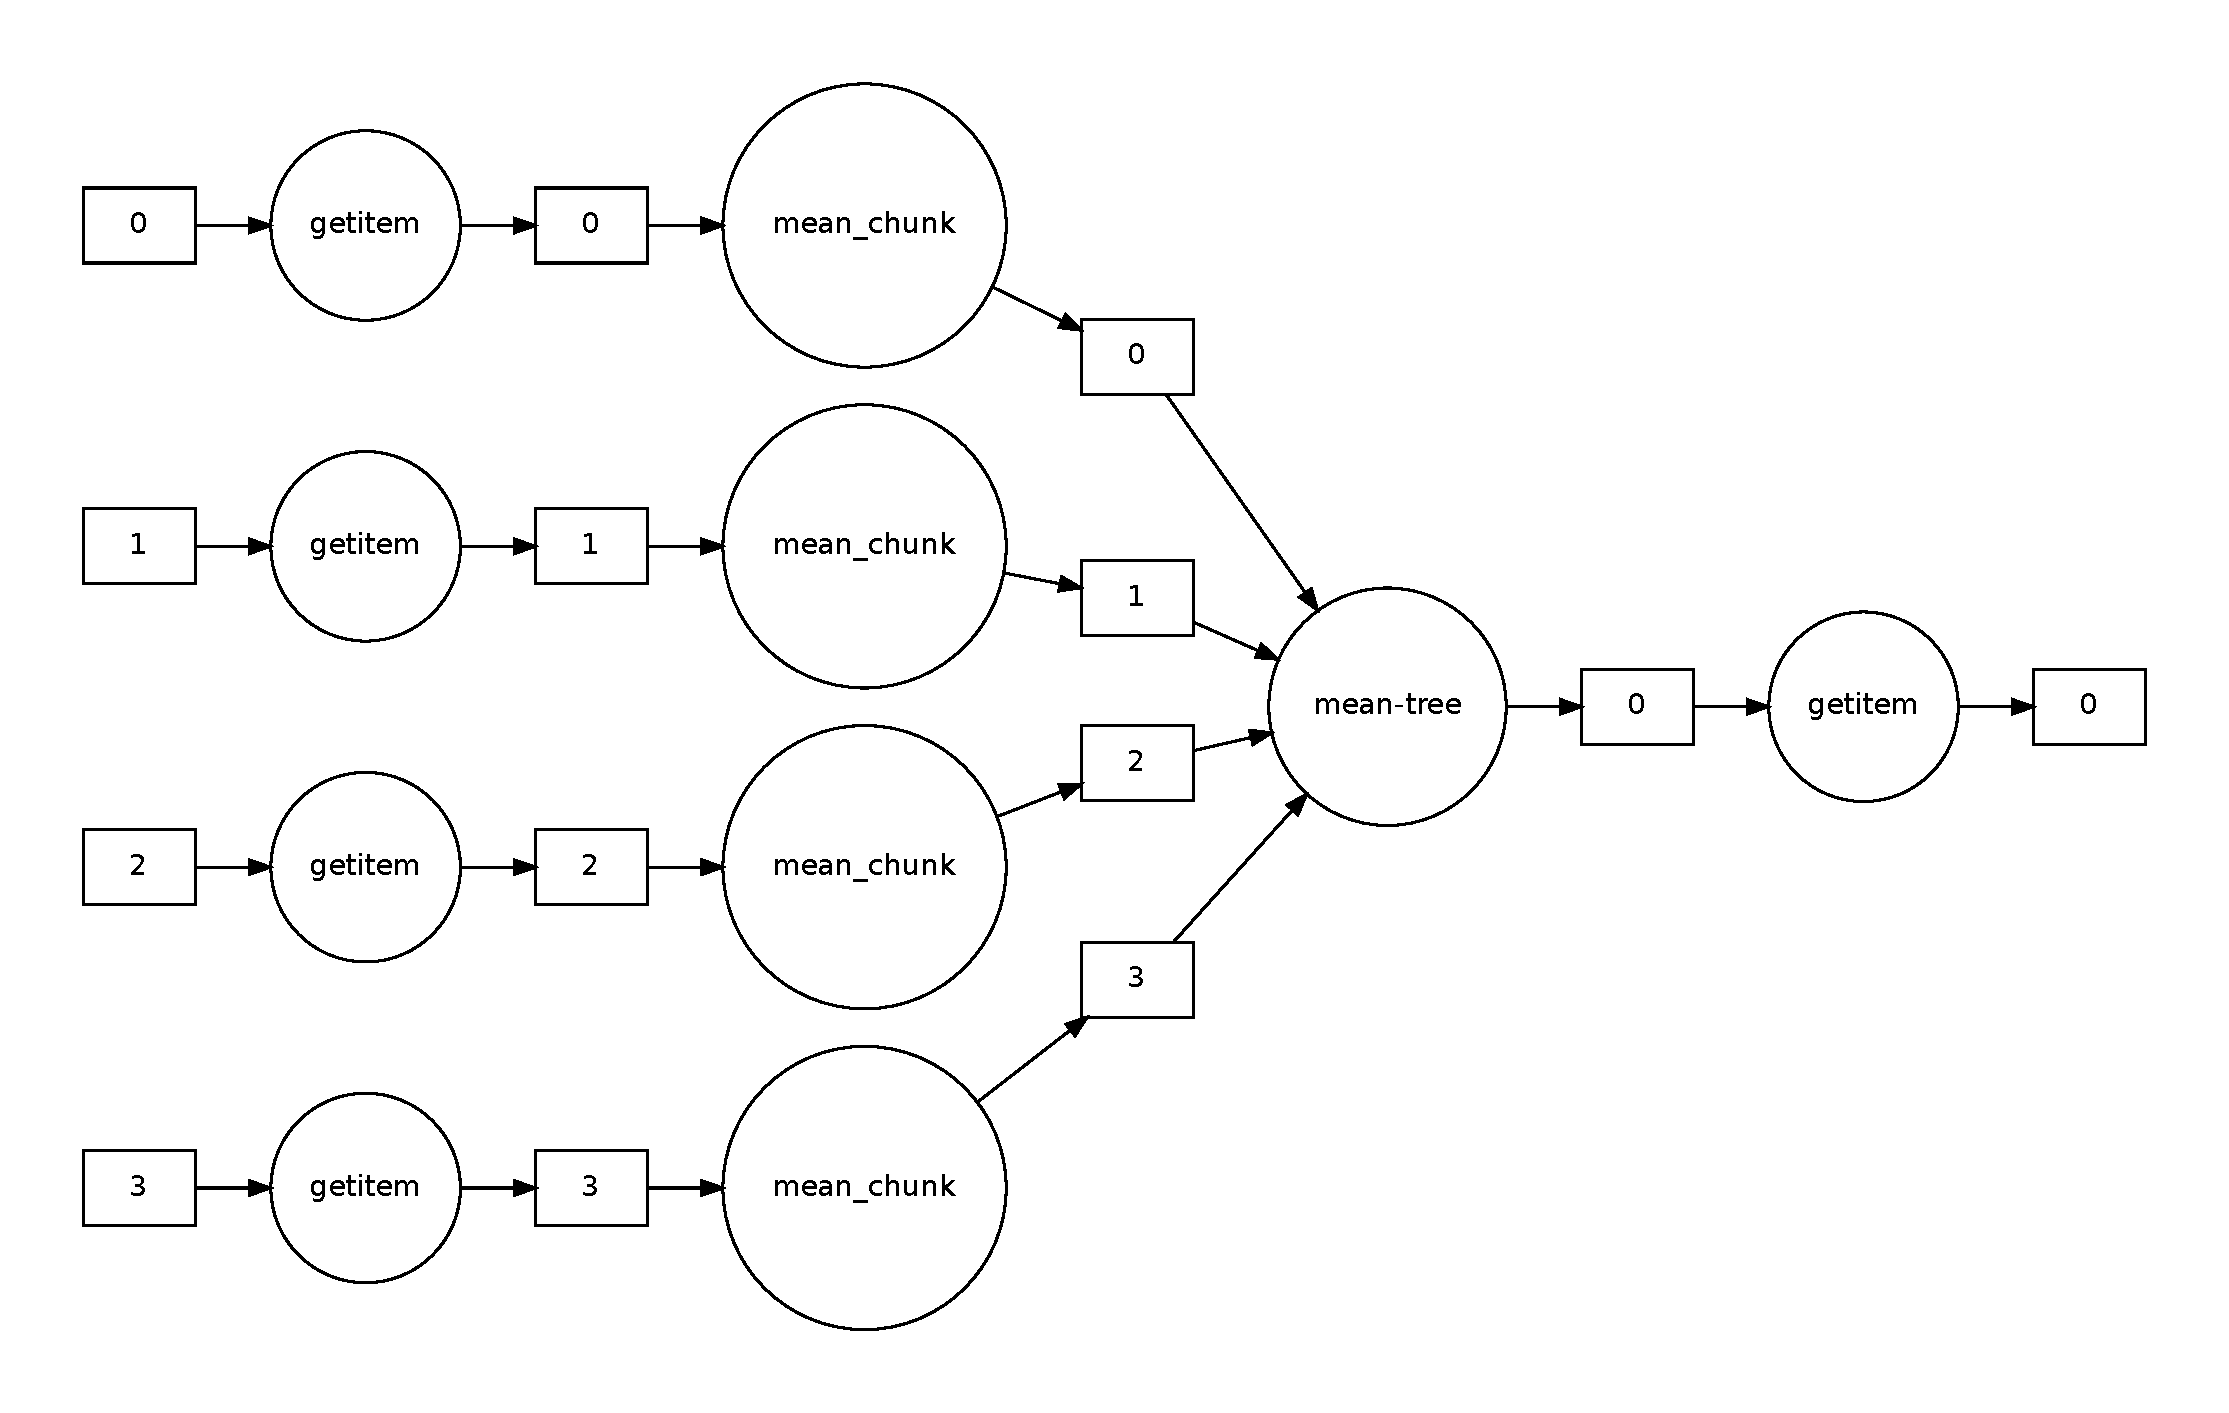
\includegraphics[width=\linewidth]{imgs/dask-dataframe-1-graph}
	\end{minipage}
\end{listing}

Specialized types of task graphs are also commonly used to parallelize \emph{dataframe}
processing, which is a popular approach for performing exploratory data analytics and
\gls{olap} queries over two-dimensional tabular datasets (dataframes). Tools such as
\dask{} DataFrame~\cite{dask}, Modin~\cite{modin},
Vaex~\cite{vaex} or CuDF~\cite{cudf} offer e.g.\ Python
\glspl{api} or \gls{sql} interfaces for expressing queries over
dataframes, and then translate these queries into task graphs that are executed on parallel
machines, distributed clusters or \gls{gpu} accelerators. Users of these tools do not
even necessarily have to know that they are interacting with task graphs, since their usage is
mostly an internal implementation detail. \Autoref{lst:dask-dataframe-example-1} shows a short Python program that
leverages the \dask{} DataFrame \gls{api} for performing a query on a
dataframe loaded from a \gls{csv} file. The query is internally translated by
\dask{} to the task graph shown on the right side of the figure, which can then be
executed e.g.\ on a distributed cluster.

While MapReduce, DataFrame processing or other similar models are useful for computations that have
a predictable structure, they are not always general enough to express complex
\gls{hpc} scientific workflows. We will thus further only consider tools and models
that allow executing arbitrary task graphs. Note that while DataFrame processing is often used
inside scientific workflows, it typically represents only a certain part of the workflow (e.g.\ a
single task or a set of tasks), and it is not used to define the structure of the whole workflow.

\subsection{Task granularity}
\label{sec:task-granularity}
Another important aspect of tasks is their \emph{granularity}. It is based on how much work
the task performs, and it also determines into how many subtasks it could be potentially divided.
In the extreme case, a \emph{coarse-grained} (low granularity) task could represent the whole computation that we
want to perform, while a \emph{fine-grained} (high granularity) task could represent only the execution of a
single \gls{cpu} instruction. With an increasing granularity, the task performs less
work, and the whole computation will thus have to be divided into a larger number of tasks. This
makes it easier to parallelize the computational workflow, yet it also increases the overall
overhead introduced by the task runtime, which has to manage and schedule more tasks. The same
properties also apply inversely for a decreasing granularity of tasks.

Since tasks can represent arbitrary computations, it is not always straightforward to determine how
they could be subdivided into multiple tasks based on their structure, and therefore how granular
they are. Usually, it is much simpler to use a proxy metric for task granularity, based on the
duration that it takes to execute a task. Therefore, if a task is very fast to execute, we will
consider that it is highly granular, while if a task takes a long time to execute, we will consider
that it has low granularity.

Task granularity is important primarily because it determines how efficiently a task graph can be
parallelized and if it even makes sense to distribute it to multiple nodes at all. For example, if
certain tasks would take mere nanoseconds to execute, there would be no point in dynamically load
balancing them across multiple distributed nodes, because the overhead of doing so would dwarf the
execution time of the tasks themselves, due to the latency induced by the network communication. In
other words, it would be faster to just execute all such tasks on the local node, rather than
sending them across the network. It could still be worth it to distribute a large number of such
extremely granular tasks to multiple nodes, but the distribution would need to happen in an
amortized way, for example only once at the beginning of the computation, to avoid the excessive
overhead.

Some task-based programming models focus primarily on high granularity tasks, for example
StarPU~\cite{starpu}, Cilk~\cite{cilk}, HPX~\cite{hpx},
PaRSEC~\cite{parsec}, Legion~\cite{legion}, TBB~\cite{tbb} or
\gls{openmp}~\cite{openmp}\footnote{Note that even though \gls{openmp} has been previously presented as an example of an
explicitly parallel model, it also offers a task system that provides facilities for implicit parallelization.}. In these models, which are
sometimes called \emph{task-parallel}~\cite{task_based_taxonomy}, tasks usually represent either
functions or blocks of code that contain a handful of instructions, and are typically relatively
quick to execute (they can run e.g.\ for milliseconds or seconds). While some of these tools also
support distributed computing, their main use-case is to provide intra-node parallelization on
multicore systems with shared memory, and often also to offload computation to attached
accelerators, such as \glspl{gpu} or \glspl{fpga}.

They can be used e.g.\ to implement high-performance numerically intensive computational kernels,
such as matrix multiplication or QR factorization~\cite{qr_factorization}, or to parallelize
recursive algorithms or algorithms with irregular data access patterns. \Autoref{lst:cilk-fibonacci}
shows a program implemented in the Cilk programming language, which calculates the n-th Fibonacci
number using a task-parallel approach.

\begin{listing}
	\begin{minted}[fontsize=\small, tabsize=4]{c}
cilk int fibonacci(int n)
{
	if (n < 2) {
		return n;
	}
	else
	{
		// Spawn a new task for each recursive call
		int x = spawn fibonaccib(n - 1);
		int y = spawn fibonaccib(n - 2);
		// Wait until the tasks finish with a barrier
		sync;
		return x + y;
	}
}
	\end{minted}
	\caption{Task-parallel Fibonacci calculation using Cilk\\Example adapted from~\cite{cilk}.}
	\label{lst:cilk-fibonacci}
\end{listing}

Task-parallel models definitely have their place in \gls{hpc}; however, they have a
different set of challenges and constraints, and they are not primarily designed to execute more
coarse-grained scientific workflows. Therefore, they are not the primary focus of this thesis.

There is also a set of task-based tools that reside at the other end of the granularity spectrum,
for example Apache Airflow~\cite{airfow}, Dagster~\cite{dagster},
Prefect~\cite{prefect} or Argo~\cite{argo}. These are commonly labeled as
\emph{Workflow Management Systems}. Although it cannot be said that there is a single distinguishing feature
that would separate these tools from other task runtimes, from my point of view these tools form a
separate category. They are primarily designed for very coarse-grained workflows with a relatively
small number of tasks, they put strong emphasis on workflow reproducibility, data provenance,
execution monitoring (typically through a web interface) and support scheduled execution (i.e.\
``run this workflow every hour''). They are also typically being applied in cloud environments,
moreso than on supercomputers. This thesis will thus not consider these tools in great detail, as
they are not primarily designed for \gls{hpc} use-cases.

\section*{Summary}
This chapter has introduced various approaches for creating distributed applications designed for
\gls{hpc} clusters. It categorized them into two broad categories, explicitly
parallel and implicitly parallel models, and demonstrated several examples of both approaches.

It has also specified the subset of distributed computing that is most relevant for this thesis. In
particular, this thesis focuses on batch processing task programming models that define
computations using fully general \glspl{dag} and that are designed for distributed
execution on an \gls{hpc} cluster, with tasks whose granularity (duration) typically
spans from milliseconds to hours.

These programming models are being commonly used for defining scientific workflows using tools that
will be described in~\Autoref{ch:sota}, which will also discuss various challenges faced by
these tools on \gls{hpc} systems. But before that, the following chapter will first
define a vocabulary of task related terms.


	\chapter{Task-based programming}
	\label{ch:taskgraphs}
	There are many ways to design and program distributed and parallel programs for HPC clusters.
Historically, a popular way of creating HPC applications was to implement the parallelization of
computation and the distribution of data explicitly, typically using message-passing (e.g.\
MPI\footnote{Message Passing Interface}~\cite{mpi}), global address space (e.g.\
PGAS\footnote{Partitioned global address space}~\cite{pgas}) and/or multithreading (e.g.\
OpenMP\footnote{Open Multi-Processing}~\cite{openmp}) frameworks, which are designed and fine-tuned
for HPC use-cases. With an explicitly parallel program, users have a lot of control over the
exchange of data and communication between individual cores and distributed nodes, which allows
them to create very performant programs. This approach is also quite flexible and enables
expressing arbitrarily complex parallelization and data distribution strategies.

However, even though such explicitly parallelized programs can be incredibly efficient,
implementing them is notoriously difficult. Deadlocks and race conditions, which are already
problematic for multithreaded programs, are even more of an issue for distributed programs. HPC
applications that use libraries for explicit distribution of data (such as various MPI
implementations) are also typically implemented in languages such as \texttt{C} or
\texttt{C++} that are infamous for making it difficult to write correct, memory-safe
programs without memory errors and undefined behaviour. This further increases the difficulty and
decreases the speed of developing correct distributed programs.

It would be unreasonable to expect that all scientists that want to leverage HPC to execute their
experiments will ``roll up their sleeves'' and spend months implementing an explicitly parallel
\texttt{C++} program that uses MPI. A more typical scenario is that scientists leverage
existing coarse-grained tools and frameworks that are optimized for HPC and use technologies like
MPI or OpenMP internally (e.g.\ GROMACS~\cite{gromacs}). However, with both the experiments
and HPC clusters becoming ever more complex each year, it is usually not sufficient to use only a
single tool. Scientific experiments require running many independent steps, which encompass data
transfer, preprocessing, postprocessing and the usage of potentially many different tools that have
to be combined. These experiments can also be executed in potentially many instances that have
different input parametrizations.

That is why in recent years, it became popular to define scientific computations using programming
models where the high-level communication and parallelization structure of the computation is
derived automatically from the program description. There are multiple ways of achieving that, such
as using e.g.\ the MapReduce~\cite{mapreduce} model, however this thesis focuses on one
approach in particular -- scientific workflows, also called pipelines. Workflows can describe a
complex computation composed of potentially many different tool invocations that can depend on one
another. They are often written in very high-level languages, such as Python, which allows users to
focus on defining the computation easily and also to quickly prototype. Crucially, these workflows
are typically based on a programming model that does not require explicit implementation of data
exchange and parallelism -- the task-based programming model.

The task-based programming model allows users to describe the high-level structure of the
computations that they want to perform using a \emph{task graph}. Users create the task graph
by splitting their desired computation into a set of \emph{tasks}, atomic and independent
computational blocks with explicitly described inputs and outputs that can be executed in a
self-contained way. Additional constraints can also be encoded into the task graph, e.g.\ which
data should be transferred between the individual tasks, which tasks cannot be executed until some
other task finishes its execution, or the necessary properties of an environment in which a task
will be executed.

The primary benefit of describing a computational workflow in such a way is that the resulting
program is \emph{implicitly parallel}. The author of the program does not imperatively specify how
should the computation be parallelized or when and how should data be exchanged. They merely
declaratively describe the individual parts of the program that can theoretically be executed in
parallel (the tasks) and then pass the task graph to a dedicated execution tool that executes the
tasks on a parallel machine (or even on a distributed cluster). Since the program is represented
with an explicit graph, the execution tool can effectively analyze its properties (or even optimize
the structure of the graph) in an automated way, and extract the available parallelism from it
without requiring the user to define parallelization opportunities explicitly.

Note that from the perspective of a task execution tool, each task is an opaque element. The tool
knows how to execute it, but it typically does not have any further knowledge of the inner
structure of the task. Therefore, the only parallelization opportunities that can be extracted by
the tool have to be expressed by the structure of the task graph. A task graph containing a single
task is thus not very useful on its own.

The task-based programming model is central to the topic of this thesis, and thus this chapter will
define various terms and concepts related to it. Note that there are many variations of this
programming model, based on the specific tool or environment where it is used, and thus the term
\emph{task-based programming} is heavily overloaded. It is used in various related technologies, ranging
from fine-grained tasks that execute a single function or just a handful of
instructions~\cite{starpu,openmp} to coarse-grained task workflows that execute binaries which
can run for hours or even days~\cite{dask, snakemake, nextflow}. This thesis primarily focuses on the latter
type of task graphs, which represent very general computations (either functions or binaries) with
various levels of granularity, that are intended to be distributed among multiple nodes of a
distributed cluster. A further distinction can be made between batch-oriented workflows, which
define a computation with a clearly delimited set of inputs that is already available when the
workflow starts, and which focus primarily on throughput, and streaming-oriented workflows, which
operate continuously on streams of input data that arrive just-in-time, and which usually focus on
latency. This thesis focuses exclusively on batch workflows, which are more common in HPC
scenarios\todo{cite}.

The term \emph{task} is also heavily overloaded in various areas of computer science, as
it is used for many unrelated concepts, from an execution context in the Linux operating system,
through a block of code executed by the OpenMP library, to a program executed by a complex
distributed computational workflow. Even in the area of distributed computing, the terminology can
vastly differ between different task execution tools and theoretical works.

Even though task-related terms can have a lot of different meanings, depending on the context, and
an attempt of providing a single unifying task theory would need to gloss over many important
details, it is still useful to provide a shared vocabulary of terms for this thesis. This chapter
thus defines several task-related terms in a way that allows capturing the specifics of task
execution in HPC environments, further described in Chapter~\ref{ch:challenges}, and that is
general enough so that it can be mapped to concepts used by task execution tools that will be
described in later chapters.

\section{Task graph}
A computational workflow in the task-based programming model is represented with a directed acyclic
graph (DAG) that we will label as a \emph{task graph}. From a high-level perspective, it
describes which individual steps should be performed, what are the constraints for where and in
which order are they computed and how should data be transferred between the individual steps of
the workflow.

There are many variations of task graphs, based on the computational properties that they are able
to describe. In the most basic form, task graph vertices represent computations to be performed,
and the edges represent dependencies between the computations, which enforce an order in which will
the computations be performed. However, numerous other concepts can also be encoded in a task
graph. For example, in addition to dependencies, the edges could represent abstract communication
channels, through which the outputs of one computation are transferred to become the inputs of
another computation that depends on it. There could be a special type of edge which specifies that
the outputs of a computation will be streamed to a follow-up computation, instead of being
transferred only after the previous computation has finished. There could also be e.g. a special
type of node that defines iterative computation that is performed repeatedly until some condition
is met.

The exact semantics of vertices and edges of task graphs depend heavily on the specifics of tools
that implement them, and thus it is not possible to have a single definition that would fit all
variants used ``in the wild''. To provide a general description, we will formally define a task
graph designed for batch workflows, which can capture the structure of dependencies between
computations and the notion of transferring data between them. This definition is general enough so
that it can be mapped to the task execution tools described later in this thesis.

A task graph is a tuple $(T, O, E)$, where $T$ is a set of
\emph{tasks}, $O$ is a set of \emph{data objects} and
$E \subseteq ((T\times{}O) \cup (O\times{}T))$ is a set of arcs. $(T \cup O, E)$ forms a finite directed acyclic
graph. The graph is structured in a way so that for every data object, there is exactly one task
that produces it: $\forall o\in{}O: (\exists t_1\in{}T: (t_1, o) \in E \land
	(\forall
	t_2\in{}T: (t_2, o) \in E \Rightarrow t_1 = t_2))$.

Below we will define several terms and properties that will be useful for working practically with
task graphs:
\begin{enumerate}
	\item If there is an arc between a task and a data object ($(t,o) \in (T\times{}O)$), then we call
	      $t$ the \emph{producer} of $o$ and $o$
	      the \emph{output} of $t$.
	\item If there is an arc between a data object and a task ($(o,t) \in (O\times{}T)$), then we call
	      $t$ the \emph{consumer} of $o$ and $o$
	      the \emph{input} of $t$.

	\item Let us introduce a binary relation $D_r$ over the set of tasks:
	      $\{(t_1, t_2): (t_1, t_2)\in{}(T\times{}T)\land t_1 \neq t_2 \land
		      \exists{}o\in{}O: (t_1, o)\in{}E
		      \land (o, t_2)\in{}E\}$. When $(t_1, t_2) \in D_r$, we say that $t_2$
	      \emph{directly depends} on $t_1$. We can also state that $t_2$
	      consumes the output produced by $t_1$.

	\item Let us introduce a binary relation $D$ over the set of tasks. Tasks
	      $t_1$ and $t_n$ are in this relation if there is a sequence
	      $(t_1, t_2, \ldots, t_n)$ such that $\forall i \in \{
		      1,2,\ldots,n - 1\}: (t_i, t_{i+1}) \in D_r$. When $(t_1, t_2) \in D$, we say that
	      $t_2$ \emph{depends} on $t_1$ and that
	      $t_1$ is a \emph{dependency} of $t_2$.

	\item We label tasks without any dependencies \emph{source tasks}. $S = \{ t \mid t\in{}T \land \forall{}t_d\in{}T:
		      (t_d, t)\notin D\}$. It is a
	      simple observation that unless the task graph is empty ($(T\cup{}O) = \emptyset$), there is always at
	      least one source task in the graph, because the graph is acyclic.
	\item We label tasks that are not depended upon by any other task \emph{leaf tasks}.
	      $L = \{ t \mid t\in{}T \land \forall{}t_d\in{}T: (t,
		      t_d)\notin D\}$.
\end{enumerate}

An example of a simple task graph is shown on Figure~\ref{fig:task-graph-example}. Tasks are represented
as circles, data objects as (rounded) rectangles\footnote{This representation will be used in all following task graph diagrams.} and arcs as arrows. The
source task $t_0$ generates two data objects, which are then used as inputs for
four additional tasks. The outputs of these four tasks are then aggregated by a final task
$t_5$. This can correspond e.g.\ to a workflow where $t_0$
generates some data, $t_{1-4}$ performs some calculation on that data and
$t_5$ performs some post-processing step and stores the results to disk.

\begin{figure}[h]
	\centering
	\resizebox{!}{35mm}{
	\begin{tikzpicture}
            \graph[
                grow right sep=6mm,
            ] {
                "$t_0$"[task] -> {
                    "$d_{0a}$"[data] -> {
                        "$t_1$"[task] -> "$d_{1}$"[data],
                        "$t_2$"[task] -> "$d_{2}$"[data],
                        "$t_3$"[task] -> "$d_{3}$"[data]
                    },
                    "$d_{0b}$"[data] -> {
                        "$t_4$"[task] -> "$d_{4}$"[data]
                    }
                } -> "$t_5$"[task]
            };
        \end{tikzpicture}
	}
	\caption{Simple task graph with six tasks and six data objects}
	\label{fig:task-graph-example}
\end{figure}

Note that the presented definition of a task graph does not describe its semantics -- how will the
graph be created and executed and what will be the interactions between tasks and data objects.
This depends on the specific tool or framework which uses task graphs to define its programming
model. For example, in a distributed batch oriented setting, if a task $t_2$
depends on another task $t_1$, then $t_2$ cannot start to execute
until $t_1$ has finished executing and the data objects produced by
$t_1$ have been transferred to the computational node that will execute
$t_2$.

\emph{Data object} is commonly represented as a serialized blob of data that has to be
transferred from the node where its producer was computed to the node where its consumer is to be
executed. If a task programming model does not encode any direct transfer of data between tasks,
then the data objects serve simply as ``empty'' markers of dependencies, and they do not hold any
actual data. In that case, we could even remove them from the task graph completely, and represent
direct dependencies with arcs between tasks.

\emph{Task} is a serializable description of a computation that can be executed
repeatedly. The serializability property is crucial, as it allow us to treat computations as data,
which is quite powerful, because it allows tasks to be sent between different nodes in a cluster or
stored to disk and to be transparently recomputed an arbitrary number of times. Tasks might need to
be recomputed e.g.\ after some failure occurs during their execution.

In practice, a single task will typically represent either the invocation a function (a block of
code that can be executed in a self-contained way) or the execution of a program (an executable
binary). Multiple tasks in a task graph can execute the same function or executable, and this is in
fact the common case, as task graphs are often used to parametrize a single computation with many
different input parameters.

Even though in the formal definition the inputs and outputs of tasks are sets, in practice they are
usually represented either with ordered sequences or some mapping that associates a name with each
input or output, because it is important to distinguish the identity and/or the order of each input
and output. For functions, inputs are its arguments, and output is its return value, which can be
structured so that a sequence of outputs is generated, instead of just a single output. For binary
programs, inputs are e.g.\ command-line arguments or the content of its \texttt{standard input stream}, and
the output can be e.g.\ the content of the \texttt{standard output stream} generated by the executed
program.

While inputs and outputs explicitly describe how data flows in and out of tasks, when a task is
executed, it can additionally also read the state of the environment in which it is being executed,
or change the state in a way that is observable by other tasks. For example, a function can read or
modify the value of a global variable, or an executable can read an environment variable or create
a file on a disk which is not specified as a task output. Such actions, which we will label as
\emph{side effects}, are typically not encoded within the task graph. Tasks should ideally
contain as few side effects as possible, because they can make task execution non-deterministic, by
causing it to produce different outputs when executed multiple times, which might not be desired.
To actually produce some output, most task graphs will eventually store some data to a file-system,
which can be either considered a side effect, or a first-class operation, depending on the
semantics of the task execution tool.

Apart from specifying the structure of required inputs and produced outputs, tasks can also define
various constraints for the environment in which they will be executed. We will use the term
\emph{resource requirements} for such constraints. As an example, a task that performs training of a
machine learning model might require a GPU (Graphics Processing Unit) to be present on the
computational node where the task will be executed. Other resources might include e.g.\ a minimum
required amount of memory (RAM) or a required amount of processor cores necessary to execute the
task.

\section{Task graph execution}
Task graphs merely describe some computation, therefore they have to be executed in order to
actually produce some results (outputs). This is the responsibility of a \emph{task runtime}, a
tool that analyzes task graphs and executes them in some \emph{computational environment}, e.g.\ a personal
computer or a distributed cluster. Such an environment contains a set of computational providers
that are able to execute tasks, these providers are commonly labeled as \emph{workers}. The
\emph{execution} of a task is the act of performing its described computation by a specific
worker (or a set of workers) with specific input(s), and producing some output(s).

There are many existing task runtimes, with varying architectures, features and trade-offs, which
affect factors like performance, fault tolerance or expressivity of the supported variant of the
task-based programming model. Some of these existing runtimes will be described in more detail in
Chapter~\ref{ch:sota}. We will consider a common scenario in the rest of this chapter,
which is a distributed task runtime with a centralized management component and a set of workers
that communicate with it via network or inter-process comunication.

In general, a task runtime manages and monitors all aspects of task graph execution; primarily it
manages tasks and workers. This agenda can be quite complex especially in a distributed setting,
where the workers operate on remote computational nodes connected by a network.

Worker management involves handling the lifetime of workers (their connection/disconnection),
facilitating data transfers between them or providing resiliency in case of worker failures. A
single worker is typically a program running on a computational node, which is connected to the
management component of the runtime. It receives commands from it, executes tasks and sends
information about task execution status back to it. Each worker typically manages some hardware
resources that are available for tasks during their execution. Hardware resources can be assigned
to workers in various ways. There can be a single worker per whole computational node, or there
could be multiple workers per node, each one managing a subset of the available resources (e.g.\ a
worker per CPU core).

The second main aspect that has to be handled by the runtime is the management of tasks. It has to
keep track of which tasks have already been computed, which tasks are currently being executed on
some worker(s) or which tasks are ready to be executed next because their dependencies have already
been computed. Two important responsibilities in this area are fault tolerance and scheduling.

Fault tolerance is the ability to gracefully handle task execution failures, and provide ways of
retrying failed computations. When the execution of a task fails with some error condition (e.g.\
because a worker executing the task crashes), a fault-tolerant task runtime will be able to
transparently restart it by launching a new execution of that task. We will use the term
\emph{task instance} for a specific execution of a task. Runtimes might impose some limits on
retrying failed tasks, e.g.\ by attempting to execute up to a fixed amount of task instances for
each task before giving up, to avoid endless failure loops.

Tasks are usually considered to be atomic from the perspective of the runtime, i.e.\ they either
execute completely (and successfully), or they fail, and then they have to be restarted from
scratch. Granularity thus plays an important factor here -- if a task is large, then a lot of work
might have to be redone if it fails and is re-executed. Some runtimes try to alleviate this cost by
enabling task checkpointing, which is able to save a computational state during task execution and
then restore computation from it in case of a failure, thus avoiding the need to start from the
beginning.

Fault tolerance is challenging in the presence of dependencies. When a task has inputs, the runtime
might have to store them (either in memory or in a serialized format on disk) even after the task
has started executing. Because there is always a possibility that it will have to restart the task
in case of a failure, and thus it needs to hold on to its inputs. In some cases it can be a better
trade-off to avoid storing the inputs and instead re-execute the dependencies of the task (even if
they have executed successfully before) to re-generate the inputs. This can help reduce memory
footprint, albeit at the cost of time, and it also might not work well if the dependencies are not
deterministic.

Note that the fact that we are even able to execute a task multiple times is one of the core
advantages of the task-based programming model, where tasks declaratively describe a self-contained
computation that can be re-executed arbitrarily. This crucial property of tasks makes
fault-tolerant execution of task graphs possible.

\section{Task scheduling}
Arguably the most important responsibility of a task runtime, and one that gets the most attention
in research works, is \emph{task scheduling}. It is the act of deciding in which order and on which
specific workers should each task execute, in a way that optimizes some key metric. There are many
metrics that can be optimized for, such as the latency to execute specific critical tasks, but the
most common metric is \emph{makespan} -- the duration between the start of the execution of
the first task to the completion of all tasks within the task graph. Scheduling is a crucial
activity of the runtime, as it has a profound effect on the efficiency of the whole workflow
execution. We will use the term \emph{scheduler} for a component of the task runtime that is
responsible for assigning tasks to workers.

%TODO: define what is a schedule

Figure~\ref{fig:scheduling-example} shows an example of how a schedule of a simple task graph looks like,
and how a trivial change in the schedule can severely affect the resulting makespan. The figure
contains a task graph with four tasks and two data objects. The size of the circles is proportional
to the duration of the tasks and the size of the rectangles is proportional to the size of the data
objects. Let us assume that we want to schedule this task graph to a cluster with three workers
($w_0$, $w_1$, $w_2$). Two different schedules
for this situation are shown in the figure. Schedule $S_0$ assigns tasks
$t_0$ and $t_1$ to worker $w_0$, task
$t_2$ to worker $w_1$ and task $t_3$ to worker
$w_2$. The timeline of the schedule the shows execution of tasks (gray rectangles)
and receiving of a data object from another worker (green rectangles) for each individual worker.
It is clear that with the schedule $S_1$, the task graph will be computed quicker
than with schedule $S_0$, even though the only difference between the two
schedules is the tasks $t_1$ and $t_3$ were swapped between
workers $w_0$ and $w_2$. Note that the schedule timeline assumes
that a worker can overlap the computation of a task with sending/receiving a data object, which is
a reasonable feature that is commonly provided by existing task runtimes.

\begin{figure}[h]
	\centering
	\resizebox{!}{110mm}{
	\begin{tikzpicture}
            \tikzmath{
                \tzerowidth = 15mm;
                \tonewidth = 20mm;
                \ttwowidth = 25mm;
                \tthreewidth = 35mm;
                \ozerowidth = 15mm;
                \oonewidth = 30mm;
            }
            \tikzset {
                taskstyle/.style={fill=gray, text=white, draw=none},
                objstyle/.style={fill=black!60!green, text=white, draw=none},
            }

            % T0
            \node[task, taskstyle, minimum size=7.5mm] (t0) at (0, 0.5) {$t_0$};
            \node[data, objstyle, minimum size=5mm] (d0a) at (-1, -1) {$d_0$};
            \node[data, objstyle, minimum size=10mm] (d0b) at (1, -1) {$d_1$};
            \draw [arrow] (t0) edge (d0a.north) (t0) edge (d0b.north);

            % T1 and T2
            \node[task, taskstyle, minimum size=10mm] (t1) at (-2, -2.5) {$t_1$};
            \node[task, taskstyle, minimum size=12.5mm] (t2) at (0, -2.5) {$t_2$};
            \draw [arrow] (d0a) edge (t1.north) (d0a) edge (t2.north);

            % T3
            \node[task, taskstyle, minimum size=17.5mm] (t3) at (2, -2.5) {$t_3$};
            \draw [arrow] (d0b.south) edge (t3.north);

            % Move below to draw the timelines
            \tikzset{shift={(-4,-4)}}

            \node[anchor=west] at (0, 0) {Schedule $S_0$: $w_0$=\{$t_0$, $t_1$\}, $w_1$=\{$t_2$\}, $w_2$=\{$t_3$\}};

            \tikzset{shift={(0,-0.75)}}
            \node (tim1A) at (0, 0) {$w_0$};
            \draw[arrow] (tim1A.east) -- ++(9, 0);
            \node[below = 0.5 of tim1A.south] (tim1B) {$w_1$};
            \draw[arrow] (tim1B.east) -- ++(9, 0);
            \node[below = 0.5 of tim1B.south] (tim1C) {$w_2$};
            \draw[arrow] (tim1C.east) -- ++(9, 0);

            % Timeline 1, row 1
            \node[taskstyle, minimum width=\tzerowidth, right = 0.2 of tim1A.east] (tim1t0) {$t_0$};
            \node[taskstyle, minimum width=\tonewidth, right = 0.1 of tim1t0.east] (tim1t1) {$t_1$};

            % Timeline 1, row 2
            \node[objstyle, minimum width=\ozerowidth, below = 1 of tim1t1.west, anchor=west]
            (tim1o0) {$d_0$ ($w_0$)};
            \node[taskstyle, minimum width=\ttwowidth, right = 0.1 of tim1o0.east] (tim1t2) {$t_2$};

            % Timeline 1, row 3
            \node[objstyle, minimum width=\oonewidth, below = 1 of tim1o0.west, anchor=west]
            (tim1o1) {$d_1$ ($w_0$)};
            \node[taskstyle, minimum width=\tthreewidth, right = 0.1 of tim1o1.east]
            (tim1t3) {$t_3$};

            \draw[dashed, draw=red] (tim1t0.west) -- ++(0, -2.75) --
            ([shift=({0,-0.75})]tim1t3.east) -- (tim1t3.east);

            \node[text=red] at (4.5, -3) {Makespan};

            % Move below to draw the timelines
            \tikzset{shift={(0,-4)}}

            \node[anchor=west] at (0, 0) {Schedule $S_1$: $w_0$=\{$t_0$, $t_3$\}, $w_1$=\{$t_2$\}, $w_2$=\{$t_1$\}};

            \tikzset{shift={(0,-0.75)}}
            \node (tim2A) at (0, 0) {$w_0$};
            \draw[arrow] (tim2A.east) -- ++(9, 0);
            \node[below = 0.5 of tim2A.south] (tim2B) {$w_1$};
            \draw[arrow] (tim2B.east) -- ++(9, 0);
            \node[below = 0.5 of tim2B.south] (tim2C) {$w_2$};
            \draw[arrow] (tim2C.east) -- ++(9, 0);

            % Timeline 2, row 1
            \node[taskstyle, minimum width=\tzerowidth, right = 0.2 of tim2A.east] (tim2t0) {$t_0$};
            \node[taskstyle, minimum width=\tthreewidth, right = 0.1 of tim2t0.east] (tim2t1)
            {$t_3$};

            % Timeline 2, row 2
            \node[objstyle, minimum width=\ozerowidth, below = 1 of tim2t1.west, anchor=west]
            (tim2o0) {$d_0$ ($w_0$)};
            \node[taskstyle, minimum width=\ttwowidth, right = 0.1 of tim2o0.east] (tim2t2) {$t_2$};

            % Timeline 2, row 3
            \node[objstyle, minimum width=\ozerowidth, below = 1 of tim2o0.west, anchor=west]
            (tim2o1) {$d_0$ ($w_0$)};
            \node[taskstyle, minimum width=\tonewidth, right = 0.1 of tim2o1.east] (tim2t3) {$t_1$};

            \draw[dashed, draw=red] (tim2t0.west) -- ++(0, -2.75) --
            ([shift=({0,-1.75})]tim2t2.east) -- (tim2t2.east);
        \end{tikzpicture}
	}
	\caption{Simple task graph and two different schedules}
	\label{fig:scheduling-example}
\end{figure}

Optimal scheduling of tasks to workers is NP-hard~\cite{Ullman1975}, even in the most basic
scenarios, when the exact duration of executing each task is known, and even if we do not consider
network costs of transferring data between workers. Task runtimes thus resort to various heuristics
tailored to their users' needs. Some classic task scheduling heuristics and their comparisons can
be found in~\cite{hlfet1974,kwok1998benchmarking,hagras2003static,wang2018list,estee}.

The scheduling heuristics have to take many factors into consideration when deciding on which
worker should a task execute:

\begin{description}
	\item[\textbf{Resource requirements}] The scheduler should respect all resource requirements specified by individual tasks. The runtime
		thus has to observe the (dynamically changing) available resources of each worker and schedule
		tasks accordingly to uphold their requirements. This can be challenging especially in the presence
		of complex resource requirements.
	\item[\textbf{Data transfer cost}] If the runtime operates within a distributed cluster, one of the most important scheduling aspects
		that it needs to consider is the transfer cost of data between workers over the network. All
		benefits gained by computing a task on another worker to achieve more parallelization might be lost
		if it takes too much time to send the data (task outputs) to that worker.

		The scheduler thus has to carefully balance the communication-to-computation ratio, based on the
		available network bandwidth, sizes of outputs produced by tasks and the current utilization of
		workers.
	\item[\textbf{Scheduling overhead}] The overhead of computing the scheduling decisions itself also cannot be underestimated. As already
		stated, computing an optimal solution is infeasible, but even heuristical approaches can have
		wildly different performance characteristics. Producing a lower quality schedule sooner, rather
		than a higher quality schedule later, can be sometimes beneficial, as we have demonstrated
		in~\cite{estee, rsds}.
	\item[\textbf{Memory consumption}] It is desirable to execute as many tasks in parallel on a given worker (with respect to its
		available parallelism), to speed up the completion of the whole workflow. However, the scheduler
		must also balance the amount of executing tasks according to the total memory that they consume. In
		general, it is quite hard to predict for how long will a task execute, and how much (peak) memory
		will it consume. When a task executes longer than expected, the workflow will still be computed, it
		will just take more time. But when a task uses more memory than expected, the scheduler puts many
		such tasks on a worker, and the worker then runs out of memory, the worker will probably crash. If
		this happens repeatedly, it can stall or completely stop the execution of the workflow. For these
		kinds of memory-intensive workflows, the scheduler should assign fewer tasks at the same time to a
		single worker, or reduce memory consumption in some other way, e.g.\ by keeping less cached data
		objects in worker's memory.
\end{description}


	\chapter{State of the Art}
	\label{ch:sota}
	There is a large body of tools designed for executing arbitrary task graphs on diverse computing
platforms, ranging from consumer-grade laptops, through cloud deployments, to distributed and
\gls{hpc} clusters. They are known under various terms, such as workflow
management systems, job managers, distributed job schedulers or orchestrators. We will use the term
\emph{task runtime} for all such task execution tools in this thesis, as has already been
discussed in the previous chapter.

Examples of such task runtimes include e.g.\ \dask{}~\cite{dask},
Parsl~\cite{parsl}, Ray~\cite{ray},
PyCOMPSs~\cite{pycompss}, HyperLoom~\cite{hyperloom},
Pydra~\cite{pydra}, Snakemake~\cite{snakemake},
SciLuigi~\cite{sciluigi}, Merlin~\cite{merlin},
Autosubmit~\cite{autosubmit}, NextFlow~\cite{nextflow},
StreamFlow~\cite{streamflow}, AiiDA~\cite{aiida},
FireWorks~\cite{fireworks} or Apache Airflow~\cite{airfow}. Each task
runtime defines its own instance of a task-based programming model, and has a different set of
trade-offs in areas such as performance and scalability, fault tolerance, data provenance,
ease-of-use, ease-of-deployment and others.

Since this thesis focuses on the ergonomics and performance aspects of executing task graphs on
\gls{hpc} clusters, this chapter discusses various challenges, bottlenecks and
shortcomings that arise when the existing task runtimes are used for this specific use-case. It
describes a set of constraints that stem both from the inherent complexity and idiosyncrasies of
\gls{hpc} software and hardware, and also from the sheer computational scale
required to efficiently utilize \gls{hpc} resources. In addition, it also mentions
various desired properties and features of task runtimes that could alleviate the mentioned
challenges.

\section{Allocation manager}
\label{sec:allocation-manager}
Users of \gls{hpc} clusters are not typically allowed to directly perform
arbitrary computations on the computational nodes (machines designed to perform expensive
computations) of the cluster. Instead, they connect to machines that are usually called
\emph{login nodes}, from which they have to enqueue their desired computation into a queue
handled by a submission system that manages the hardware resources of the cluster. We will use the
term \emph{allocation manager} for these submission systems and the term
\emph{allocation}\footnote{The term \emph{job} is also commonly used for the concept of
\gls{hpc} computational requests.} for a computational request submitted by a
user into these managers.

Allocation managers are required for providing fair access to the resources of the cluster, because
\gls{hpc} clusters are typically used by many people at the same time. Without a
centralized management, hardware resources could be inadvertently shared amongst multiple users at
once, which could have undesirable performance and security implications, and could lead to
oversubscription. Furthermore, usage of these clusters is usually metered. Users can typically only
use a certain amount of resources assigned to their \emph{computational project}, and when their
resources run out, they have to ask (or pay) for more resources. Allocation managers thus also
implement user and project accounting, so that there is a clear historical record of how many
resources were consumed by individual users of the cluster.

The majority of \gls{hpc} clusters~\cite{slurm-schedmd} use one of the two
most popular allocation manager implementations, either Slurm~\cite{slurm} or
\gls{pbs}~\cite{pbs}\footnote{Or some of its many derivatives,
such as TORQUE~\cite{torque} or OpenPBS~\cite{openpbs}}. For simplicity,
Slurm will be used as a default representative of allocation managers in the rest of this thesis
(unless otherwise noted), since it shared all the important described constraints with
\gls{pbs}.

The following process describes how computations are typically executed on
\gls{hpc} clusters that use an allocation manager:

\begin{enumerate}
	\item The user enqueues a computational request (allocation) into the manager from a login node. The
	      request typically has to specify at least how many nodes should be allocated and what is the
	      maximum duration of the computation (usually labeled as \emph{wall-time}), after which the
	      computation will be forcibly stopped by the manager. It can also contain additional configuration,
	      such as what kinds of nodes should be allocated or what is the priority of the request.
	\item The allocation manager puts the request into a queue and schedules it to be executed at some time
	      in the future. Since users submit their allocations into the manager continuously, each allocation
	      has different properties and priorities, and it is not possible to precisely predict for how long
	      will an allocation run, the schedule can be quite dynamic, so users might have to wait seconds,
	      minutes, hours or even days before their allocation starts to execute.
	\item Once the allocation gets to the front of the queue and there are enough resources available, the
	      manager provisions the requested amount of hardware resources (typically a number of whole
	      computational nodes) and either executes a script (a \emph{batch} allocation) or
	      provides the user with an interactive terminal session on one of the allocated nodes (an
	      \emph{interactive} allocation). Allocations are often configured in a way that provides
	      their authors with exclusive access to the allocated hardware resources, in which case no other
	      user will be able to use these resources (nodes) until the allocation finishes.
	\item Once the executed script finishes (or the wall-time duration is reached), the allocation ends, and
	      its hardware resources are released so that they can be used by another allocation in the future.
\end{enumerate}

Although it might not be obvious from the above description at first, the presence of an allocation
manager actually presents perhaps the largest obstacle for ergonomic execution of task graphs on
\gls{hpc} systems. Instead of executing their task graphs directly, users have to
think about how to split the task graph into allocations and then submit them. While this is true
of any computation executed on \gls{hpc} clusters in general, in the case of task
graphs it is especially difficult because of their complex structure.

To execute a task graph using an allocation manager, it is necessary to find a way how to map tasks
to allocations, ideally in a way that efficiently utilizes \gls{hpc} resources and
is as transparent as possible for the users. There are several ways of performing this
task-to-allocation assignment, which will be described below, along with a set of challenges and
limitations that are mostly caused by various performance bottlenecks of existing allocation
managers.

\subsection*{Execute the whole task graph in a single allocation}
At first, it might seem that executing a task graph within a single allocation is a simple
solution, since all the user has to do is submit an allocation that will eventually execute the
complete task graph (using some task runtime), which is a similar approach that would be used for
executing the task graph e.g.\ on a personal computer.

And it indeed is simple -- when it is possible at all. The problem is that allocation managers tend
to place fairly strict limits on the maximum possible execution duration of an allocation (the
wall-time) and also on the number of resources (nodes) that can be requested at once, to ensure a
fairer assignment of resources to users of a cluster. Therefore, when a task graph has too many
tasks, takes too long to execute, or the user wants to leverage more computational resources than
can fit in a single allocation, this approach will not work.

In a way, if the task graph computation is short enough that it can fit within a single allocation,
it might not always even make sense to use an \gls{hpc} cluster to compute it. A
more realistic scenario is that even if an individual task graph can be executed quickly, users
might want to execute many such task graphs (for example to execute many experiments with different
parametrizations). This situation can be seen as a special case of a large task graph that consists
of many disjoint components (smaller task subgraphs). In this case, it will again typically not be
possible to execute all such task graphs inside a single allocation.

Even when a task graph can be reasonably executed within a single allocation, this approach might
lead to underutilization and waste of resources. Consider a typical data analysis or a machine
learning workflow that works in several stages. First, it loads a dataset from disk and
pre-processeses it, then it trains a machine learning model, and finally it performs some
post-processing step, which e.g.\ analyzes the resulting model. The pre-processing and
post-processing steps are usually not very resource intensive and run on \glspl{cpu}
only, while the training step typically consumes a lot of resources and is usually executed on a
\gls{gpu} accelerator. To execute such a workflow, we will need to ask for a set
of resources that contain such an accelerator. The issue is that all resources of an allocation are
reserved for its whole duration, therefore we will have to pay the price for the expensive
accelerated nodes (and prevent others from using them) even during the execution of workflow steps
in which they will be underutilized or completely idle. This is caused by the fact that all
allocated resources are tied to the lifetime of the whole allocation.

One additional disadvantage of this approach is queue latency. Large allocations that require a
long wall-time duration and/or request many computational nodes typically spend a much longer time
in the allocation manager queue, because it is more difficult for the manager to make sure that all
the requested resources are available at the same time. As a concrete example, ten allocations that
require a one hour wall-time can potentially be completed much quicker than a single allocation
that requests a ten hour wall-time (and similar behavior can be expected w.r.t.\ the amount of
requested nodes), because these allocations do not need to run at the same time, therefore it is
easier for the manager to schedule them.

In terms of task runtime support, this approach can be used with essentially all existing task
runtimes, since it does not require any special support from the runtime. The user simply submits a
single allocation, and when it starts, the whole task graph is computed with a task runtime all in
one go. This approach is thus quite simple for the user, although as has been mentioned, it might
not be feasible for many use-cases, and it can lead to resource waste and a long latency before
receiving first results (finished tasks).

\subsection*{Execute each task as a separate allocation}
The previous approach mapped all tasks to a single allocation. An opposite extreme would be to map
each task to a separate allocation. This approach might seem intuitive, because from a certain
point of view, \gls{hpc} allocation managers can also be viewed as task runtimes,
if we consider allocations to be tasks, therefore it might be tempting to treat them as such. Both
\gls{pbs} and Slurm even support a crude notion of dependencies between
allocations, which could allow users to express computational graphs. Indeed, in an ideal world,
there would be no difference between an allocation manager and a task runtime, and users could
simply construct an arbitrarily granular task graph and execute it simply by submitting it directly
into the allocation manager.

However, in practice, this approach is mostly infeasible, at least with the currently popular
allocation managers (\gls{pbs} and Slurm), because they introduce a non-trivial
amount of overhead per each allocation. In an ideal scenario, Slurm is able to launch a few hundred
allocations per second~\cite{slurm-throughput}, however more realistically, users on a crowded
cluster might experience at least a few hundred milliseconds overhead per allocation, if not more,
which is order(s) of magnitude more than the overhead of a typical task
runtime~\cite{rsds}.

Even though there is probably room for reducing the overhead of contemporary
\gls{hpc} allocation managers, it is important to note that some of the
performance limitations are inherent. Allocation managers have to (amongst other things) provide
accurate accounting, handle robust and secure provisioning and cleanup of hardware resources
provided to allocations, manage user and process isolation on computational nodes and ensure user
fairness. These responsibilities are out of scope for most task runtimes, therefore it is not
surprising that they can usually achieve much higher performance. While in theory, it could be
possible to design an allocation manager that can also act as a (performant) task runtime at the
same time (and some efforts have been made on this front~\cite{flux}), it is
probably infeasible to modify the two most prominent allocation managers that are used almost
ubiquitously in the current \gls{hpc} ecosystem to support this use-case.

Due to this overhead, allocation managers usually limit the number of allocations that can be
enqueued by a single user at any given time (e.g.\ to a few hundreds or thousands), to ensure that
the manager is not overloaded and that it can continue to serve requests from other users of the
cluster. Therefore, unless the task graph is very small, most likely it will be infeasible to
create a separate allocation per each task.

It should be noted that both Slurm and \gls{pbs} allow partially overcoming this
limitation through \emph{allocation arrays} (also labeled as job arrays). This concept allows users to submit a large amount
of computations with the same shape and properties in a single allocation. However, it still has
several disadvantages. One is a lack of flexibility; it does not easily allow submitting
heterogeneous tasks with different resource requirements, and it also has only a very crude support
for dependencies between the submitted tasks. Another disadvantage is fault tolerance; if some of
the tasks of the array fail, users might have to manually identify them and resubmit them in
another allocation, which is far from effortless. And of course, clusters do impose limits also for
allocation arrays, therefore even the array approach might not be enough to encompass all tasks of
massive task graphs.

Apart from the maximum allocation count, there are other limitations that can be imposed by
allocation managers. Some tasks of scientific workflows can be quite granular, and require only a
handful of resources, e.g.\ a single \gls{cpu} core. To avoid wasting resources,
an allocation mapped to such a task should thus ask only for the exact set of resources needed by
it. However, allocation managers are sometimes configured in a way that only offers node-level
granularity of hardware resources, and thus does not allow users to request less than a whole
computational node~\cite{it4i_node_scheduling_policy}. In these cases, it would be quite wasteful if we had
to request a whole computational node e.g.\ for a simple task that runs for just a few seconds and
requires only a handful of cores.

There are two primary reasons why allocation managers limit the granularity of allocations. First,
reducing the granularity of allocations lessens the overall overhead. If users are able to ask
e.g.\ for individual cores of each node, the manager would have to manage many more allocations
than when users ask for complete nodes, which could quickly become unmanageable. The second reason
is security. If the manager provides the ability to reserve only a fraction of a node, allocations
from multiple users can execute on the same node at the same time. This reduces isolation between
users, which might potentially have security implications. It can also affect performance, since
concurrently running allocations might compete for some shared resource on the same node (e.g.\ the
operating system process scheduler). Since each node runs a single instance of an operating system,
it forms a natural isolation domain, and it is thus also frequently used as an unit of granularity
for allocations.

Another reason why using an allocation manager directly as a task runtime might be impractical is
that it makes debugging and prototyping of task graphs more difficult. It is useful to have the
ability to examine the execution of a workflow locally, e.g.\ on the user's personal computer,
before running it on a cluster. However, if the task graph would be implemented directly in an
allocation manager, users would have to deploy tools like \gls{pbs} or Slurm
locally, which can be challenging.

To sum up, using an allocation manager directly as a task runtime is impractical, primarily because
of the overhead associated with each allocation and the resulting difference in task and allocation
granularity, which can lead to resource waste. Users that want to execute a task graph on an
\gls{hpc} system thus usually use a separate task runtime rather than defining
task graphs using the allocation manager directly.

\subsection*{Partition the task graph into multiple allocations}
As we have seen, both of the mentioned extreme approaches had severe disadvantages. The remaining
approach is to devise a general task-to-allocation assignment, by partitioning the task graph into
smaller subgraphs and submitting each subgraph as a separate allocation. This approach allows to
map a large number of tasks into a smaller number of allocations, and thus amortize the allocation
overhead. Most users will probably sooner or later converge to a similar approach, once their task
graph becomes sufficiently large and complex, and they will have to reconcile the coarse-grained
nature of allocations with the fine-grained nature of tasks.

This process is far from straightforward if it is performed manually, i.e.\ if the user has to
manually split the task graph when preparing the allocations, and then start an independent
instance of a task runtime inside each allocation. In this case, users need to figure out how to
optimally partition the task graph, which is itself a notoriously difficult
NP-hard~\cite{graph_partitioning} problem in general, and then submit the subgraphs as separate
allocations.

Furthermore, this approach might require implementation efforts outside the boundaries of the used
task-based programming model, which can be cumbersome. For example, the intermediate outputs of
computed tasks of a partitioned subgraph might have to be persisted to a filesystem before the
corresponding allocation ends, and the results from multiple allocations then have to be merged
together to produce all the necessary data outputs of the complete task graph. Another issue is
that if some tasks fail, and their corresponding allocation ends, so the task runtime does not get
a chance to recompute them, users will need to identify such failed tasks and then selectively
resubmit them into new allocations, which can get complicated quickly.

In general, while this approach can overcome the limitations of executing the workflow inside a
single allocation and of using the allocation manager itself as a task runtime, it also requires
non-trivial effort from users, because they essentially have to reimplement parts of task runtime
functionality on top of the allocation manager.

% TODO: obrázky!

There are task runtimes that can help with automating a part of this effort, by operating on a
level above the allocation manager, instead of always running only within the context of a single
allocation. Thanks to this property, they are able to represent task graphs that span multiple
allocations. We will use the term \emph{meta-schedulers} for these task runtimes.

An example of such as tool is \snakemake~\cite{snakemake}, which allows users to define
complex task graphs that be executed in multiple allocations. It is also able to partition the task
graph into \emph{groups}, where all tasks of a single group are always executed inside
the same allocation. However, this partitioning has to be specified explicitly by the author of the
workflow, which can be laborious.

While automating the partitioning process is useful, a \emph{static} division of
subgraphs into allocations (be it performed manually or in an automated fashion) that has to be
decided \emph{before} the allocations are submitted might still lead to suboptimal
hardware utilization. When the individual subgraphs are executed by independent instances of a task
runtime that run in separate allocations and do not communicate with each other, it will not be
possible to load-balance tasks across different allocations, which can limit the achieved hardware
utilization.

\subsection*{Fully dynamic scheduling across allocations}
Ideally, users would not have to think about task graph partitioning (or even the allocation
manager) at all; they should be able to construct a task graph and execute it directly on an
\gls{hpc} cluster in a straightforward way, by letting the task runtime perform
the task graph partitioning and load-balancing across multiple allocations automatically for them.
This could be achieved by integrating allocation managers and task runtimes more closely. We have
seen that adding support for executing fine-grained task graphs to allocation managers is probably
not realistic, since they have too many other responsibilities. However, a promising approach is to
extend meta-schedulers, which know how to communicate with allocation managers, with dynamic
scheduling of tasks across different allocations, to enable flexible load-balancing and simple
execution of task graphs on \gls{hpc} systems.

\Autoref{ch:hyperqueue} will discuss the interaction of task graphs and allocation managers in
more detail, and describe a design for a fully dynamic mapping of tasks to allocations that can
overcome the challenges mentioned in this section.

\section{Cluster heterogeneity}
Even though task graphs are designed to be portable and ideally should not depend on any specific
execution environment, for certain types of tasks, we need to be able to describe at least some
generic environment constraints. For example, when a task executes a program that leverages the
CUDA programming framework~\cite{cuda}, which is designed to be executed on an
NVIDIA graphics accelerator, it has to be executed on a node that has such a
\gls{gpu} available, otherwise it will not work properly.

It should thus be possible for a task to define \emph{resource requirements}, which specify resources
that have to be provided by an environment that will execute such task. For example, a requirement
could be the number of cores (some tasks can use only a single core, some can be multithreaded),
the amount of available main memory, a minimum duration required to execute the task or (either
optional or required) presence of an accelerator like a \gls{gpu} or an
\gls{fpga}. In order to remain portable and independent of a specific execution
environment, these requirements should be abstract and describe general, rather than specific,
types of resources.

The challenge related to resource requirements of \gls{hpc} tasks specifically is
the diverse kinds of hardware present in modern \gls{hpc} clusters, which have
started to become increasingly heterogeneous in recent years. This trend can be clearly seen in the
TOP500 list of the most powerful supercomputers~\cite{top500analysis}. Individual cluster
nodes contain varying amounts and types of cores and sockets, main memory,
\gls{numa} nodes or accelerators like \glspl{gpu} or
\glspl{fpga}. Since \gls{hpc} software is often designed to
leverage these modern \gls{hpc} hardware features, this complexity is also
propagated to tasks and their resource requirements.

Tasks might require a combination of several requirements, for example two
\glspl{gpu}, sixteen cores and 32 GiB of main memory. They can also be designed in
a way that allows them to leverage an open-ended range of resources, e.g.\ a task might require at
least four cores, but if more are available, it could use as many as possible. And some tasks might
even support several variants of requirements, for example a task might either use four cores and a
single \gls{gpu} (if there is one available), or it could use more cores (and no \gls{gpu})
to offset the absence of an accelerator.

A resource requirement that is fairly specific to \gls{hpc} systems is the usage
of multiple nodes per single task. This requirement is necessary for programs that are designed to
be executed in a distributed fashion, such as programs using \gls{mpi}, which are
quite common in \gls{hpc}. The use-case of tasks using multiple nodes is
discussed in more detail later in this chapter.

Existing task runtimes usually support some notion of resource requirements, although they can be
somewhat limited. Some runtimes support only a fixed set of known resources (typically the number
of cores and the amount of memory), which is not enough to describe complex resources of
heterogeneous clusters. Other runtimes, such as \dask{} or
\snakemake{}, support arbitrary resources, although they do not allow expressing
more complex patterns, such as the mentioned case where a task could define multiple resource
requirement configurations. Supporting multiple nodes for a single task is not supported by most
runtimes at all, because their programming model often assumes that a each task executes on a
single node only.

To support the mentioned scenarios, task runtimes should ideally allow users to specify arbitrarily
fine-grained and abstract resource requirements for each task, with support for multiple
requirement variants per task and multi-node tasks. They should also take these requirements into
account when scheduling, both to make sure that they are upheld, but also to use this provided
information to utilize the available hardware effectively.

\section{Data transfers}
After a task is computed, it can produce various outputs, such as standard error or output streams,
files created on a filesystem or data objects that are then passed as inputs to dependent tasks.
There are many approaches to storing and transferring these outputs.

Some task frameworks store task outputs on the filesystem, since it is relatively simple to
implement and it provides support for basic data resiliency out-of-the-box. A lot of existing
software (that might be executed by a task) also makes liberal use of the filesystem, which can
make it challenging to avoid filesystem access altogether. However, \gls{hpc}
nodes often do not contain any local disks, but instead use shared filesystems that are accessed
over a network. While this can be seen as an advantage, since with a shared filesystem it is much
easier to share task outputs amongst different workers, it can also be a severe bottleneck. Shared
networked filesystems can suffer from high latency and accessing them can consume precious network
bandwidth that is also used e.g.\ for managing computation (sending commands to workers) or for
direct worker-to-worker data exchange. Furthermore, data produced in \gls{hpc}
computations can be quite large, and thus storing it to a disk can be a bottleneck even without
considering networked filesystems.

These bottlenecks can be alleviated by transferring task outputs directly between workers over the
network (preferably without accessing the filesystem in the fast path), which is implemented e.g.\
by \dask{}. Some runtimes (for example HyperLoom~\cite{hyperloom})
also leverage \gls{ram} disks, which provide support for tasks that need to
interact with a filesystem, while avoiding the performance bottlenecks associated with disk
accesses. It is also possible to use \gls{hpc} specific technologies, such as
\gls{mpi} or InfiniBand, to improve data transfer performance by fully exploiting
the incredibly fast interconnects available in \gls{hpc} clusters.

Data outputs produced by tasks tend to be considered immutable in existing task runtimes, since a
single output can be used as an input to multiple tasks, and these might be executed on completely
different computational nodes, so it would be challenging to synchronize concurrent mutations of
these objects. A problem that can arise with this approach is that if the data outputs are large,
but the computation of tasks that work with the data is short, then the serialization overhead (or
even memory copy overhead, if the dependent task is executed on the same node) can dominate the
execution time. Such use-cases can be solved with stateful data management, for example in the form
of \emph{actors}, which can be seen as stateful tasks that operate on a single copy
of some large piece of data, without the need to transfer or copy it.

\section{Fault tolerance}
Fault tolerance is relevant in all distributed computing environments, but
\gls{hpc} systems have specific requirements in this regard. As was already
mentioned, computational resources on \gls{hpc} clusters are provided through
allocation managers. Computing nodes allocated by these managers are provided only for a limited
duration, which means that for long-running computations, some nodes will disconnect and new nodes
might appear dynamically during the lifecycle of the executed workflow. Furthermore, since the
allocations go through a queue, it can take some time before new computational resources are
available, therefore the computation can remain in a paused state, where no tasks are being
executed, for potentially long periods of time.

It is important for task runtimes to be prepared for these situations; they should handle node
disconnections gracefully, even if a task was being executed on a node that is disconnected, and
they should be able to restart previously interrupted tasks on newly arrived workers. In general,
in \gls{hpc} scenarios, worker instability and frequent disconnects should be
considered the normal mode of operation, rather than just a rare edge case.

\section{Multi-node tasks}
Many existing \gls{hpc} applications are designed to be executed on multiple
(potentially hundreds or even thousands) nodes in parallel, using e.g.\ \gls{mpi}
libraries or other communication frameworks. Multi-node execution could be seen as a special
resource requirement, which states that a task should be executed on multiple workers at once.
Support for multi-node tasks is challenging, because it affects many design areas of a task
runtime:
\begin{description}
	\item[Scheduling] When a task requires multiple nodes for execution and not enough nodes are available at a given
		moment, the scheduler has to decide on a strategy that will allow the multi-node task to execute.
		If it would be constantly trying to backfill available workers with single-node tasks, the
		multi-node tasks could be starved.

		The scheduler might thus have to resort to keeping some nodes idle for a while to enable the
		multi-node task to start as soon as possible. Another approach could be to interrupt the currently
		executing tasks and checkpoint their state to make space for a multi-node task, and then resume
		their execution once the multi-node task finishes.

		In a way, this decision-making already has to be performed on the level of individual cores even
		for single-node tasks, but adding multiple nodes per task makes the problem much more difficult.
	\item[Data transfers] It is relatively straightforward to express data transfers between single-node tasks in a task
		graph, where a task produces a set of complete data objects, which can then be used as inputs for
		dependent tasks. With multi-node tasks, the data distribution patterns become more complex, because
		when a task that is executed on multiple nodes produces a data object, the object itself might be
		distributed across multiple workers, which makes it more challenging to use it in follow-up tasks.
		The task graph semantics might have to be extended with expressing various data distribution
		strategies, for example a reduction of data objects from multiple nodes to a single node, to
		support this use-case.

		When several multi-node tasks depend on one another, the task runtime should be able to exchange
		data between them in an efficient manner. This might require some cooperation with the used
		communication framework (e.g.\ \gls{mpi}) to avoid needless repeated serialization
		and deserialization of data between nodes.
	\item[Fault tolerance] When a node executing a single-node task crashes or disconnects from the runtime, its task can be
		rescheduled to a different worker. In the case of multi-node tasks, failure handling is generally
		more complex. For example, when a task is executing on four nodes and one of them fails, the
		runtime has to make sure that the other nodes will be notified of this situation, so that they can
		react accordingly (either by finishing the task with a smaller number of nodes or by failing
		immediately).
\end{description}

Most existing task runtimes only consider single-node tasks and do not provide built-in support for
multi-node tasks, which forces users to use various workarounds, for example by emulating a
multi-node task with a single-node task that uses multi-node resources that are not managed by the
task runtime itself. To enable common \gls{hpc} use-cases, task runtimes should
be able to provide first-class support for multi-node tasks and allow them to be combined with
single-node tasks in a seamless manner. Advanced multi-node task support could be provided e.g.\ by
offering some kind of built-in integration with \gls{mpi} or similar common
\gls{hpc} technologies.

\section{Scalability}
The massive scale of \gls{hpc} hardware (node count, core count, network
interconnect bandwidth) opens up opportunities for executing large-scale task graphs, but that in
turn presents unique challenges for task runtimes. Below you can find several examples of
bottlenecks that might not matter in a small computational scale, but that can become problematic
in the context of \gls{hpc}-scale task graphs.

\begin{description}
	\item[Task graph materialization] Large computations might require building massive task graphs that contain millions of tasks. The
		task graphs are typically defined and built outside of computational nodes, e.g.\ on login nodes of
		computing clusters or on client devices (e.g.\ laptops), whose performance can be limited. It can
		take a lot of time to build, serialize and transfer such graphs over the network to the task
		runtime that runs on powerful computational nodes. This can create a bottleneck even before any
		task is executed. This has been identified as an issue in some existing task
		runtimes~\cite{dask-client-perf}.

		In such case, it can be beneficial to provide an \gls{api} for defining task graphs
		in a symbolic way by representing a potentially large group of similar tasks with a compressed
		representation to reduce the amount of consumed memory. For example, if we want to express a
		thousand tasks that all share the same configuration, and differ e.g.\ only in an input file that
		they work with, we could represent this a group of tasks with a size thousand, rather than storing
		a thousand of individual task instance in memory. This could be seen as an example of the classical
		Flyweight design pattern~\cite{gof}.

		Such symbolic graphs could then be sent to the runtime in a compressed form and re-materialized
		only at the last possible moment. In an extreme form, the runtime could operate on such graphs in a
		fully symbolic way, without ever materializing them.
	\item[Communication overhead] Scaling the number of tasks and workers will necessarily put a lot of pressure on the communication
		network, both in terms of bandwidth (sending large task outputs between nodes) and latency (sending
		small management messages between the scheduler and the workers). Using \gls{hpc}
		technologies, such as \gls{mpi} or a lower-level interface like
		\gls{rdma}, could provide a non-trivial performance boost in this regard. Some
		existing runtimes, such as \dask{}, can make use of such
		technologies~\cite{dask-ucx}.

		As we have demonstrated in~\cite{pspin, spin2}, in-network computing can be also used to
		optimize various networking applications by offloading some computations to an accelerated
		\gls{nic}. This approach could also be leveraged in task runtimes, for example to
		reduce the latency of management messages between the scheduler and workers or to increase the
		bandwidth of large data exchanges amongst workers, by moving these operations directly onto the
		network card. This line of research is not pursued in this thesis, although it could serve as an
		interesting idea to be explored.
	\item[Scheduling] Task scheduling is one of the most important responsibilities of a task runtime, and with large
		task graphs, it can become a serious performance bottleneck. Existing task runtime, such as
		\dask{}, can have problems with keeping up with the scale of
		\gls{hpc} task graphs. The scheduling performance of various task scheduling
		algorithms will be examined in detail in \Autoref{ch:estee}. \autoref{ch:rsds}
		then will describe the performance overhead of the \dask{} runtime and its
		scheduler.
	\item[Runtime overhead] A typical architecture of a task runtime consists of a centralized component that handles task
		assignments, and a set of connected workers. As we have shown in~\cite{rsds}, task
		runtimes with this architecture should be mindful of their task execution and communication
		overhead. For example, even with an overhead of just $1ms$ per task, executing
		a task graph with a million tasks would result in total accumulated overhead of more than fifteen
		minutes! Our results indicate that increasing the performance of the central scheduling and
		management component of a task runtime can have a large positive effect on the overall time it
		takes to execute the whole task graph. This is explored in detail in \Autoref{ch:rsds}.

		However, the performance of the central server cannot be increased endlessly, and from some point,
		a centralized architecture will become a bottleneck. Even if the workers exchange data outputs
		directly between themselves, the central component might become overloaded simply by coordinating
		and scheduling the workers using management messages.

		In that case, a decentralized architecture could be leveraged to avoid the reliance on a central
		component. Such a decentralized architecture can be found e.g.\ in Ray~\cite{ray}.
		However, to realize the gains of a decentralized architecture, task submission itself has to be
		decentralized in some way, which might not be a natural fit for common task graph workflows. If all
		tasks are generated from a single component, the bottleneck will most likely remain even in an
		otherwise fully decentralized system.
\end{description}

\section{Iterative computation}
There are various \gls{hpc} use-cases that are inherently iterative, which means
that they perform some computation repeatedly, until some condition (which is often determined
dynamically) is satisfied. For example, the training of a machine learning model is typically
performed in iterations (called epochs) that continue executing while the prediction error of the
model keeps decreasing. Another example could be a molecular dynamics simulation that is repeated
until a desired accuracy (or other property) has been reached.

One approach to model such iterative computations would be to run the whole iterative process inide
a single task. While this is simple to implement, it might not be very practical, since such
iterative processes can take a long time to execute, and performing them in a single task would
mean that we could not leverage desirable properties offered by the task graph abstraction, for
example fault tolerance. Since the computation \emph{within} a single task is
typically opaque to the task runtime, when the task would fail, it would need then need to be
restarted from scratch.

A better approach might be to model each iteration as a separate task. In such case, the task
runtime might be able to restart the computation from the last iteration, if a failure occurs.
However, this approach can be problematic if the number of iterations is not known in advance,
since some task runtimes expect that the structure of the task graph will be immutable once the
graph has been submitted for execution.

To support iterative computation, task runtimes should allow their users to stop the execution of a
task graph (or its subgraph) once a specific condition is met, and also to add new tasks to the
task graph in a dynamic fashion, if it is discovered during its execution that more iterations are
needed. \dask{} and \ray{} are examples of task runtimes
that allow adding tasks to an existing task graph dynamically.

\section{Deployment}
Even though it might sound trivial at first, an important aspect that can affect the ergonomics of
executing task graphs (or any kind of computation, in general) on an \gls{hpc}
cluster is ease-of-deployment. Supercomputing clusters are notable for providing only a severely
locked-down environment for their users, which does not grant elevated privileges and requires
users to either compile and assemble the runtime dependencies of their tools from scratch or choose
from a limited set of precompiled dependencies available on the cluster, which can have
incompatible versions or a non-optimal configuration.

Deploying any kind of software (including task runtimes) that has non-trivial runtime dependencies,
or non-trivial installation steps, if it is not available in a pre-compiled form for the target
cluster, can serve as a barrier for using it on an \gls{hpc} cluster. Many
existing task runtimes are not trivial to deploy. For example, several task runtimes, such as
\dask{}, \snakemake{} or \pycompss{}, are
implemented in Python, a language that typically needs an interpreter to be executed, and also a
set of packages in specific versions, that need to be available on the filesystem of the target
cluster. Installing the correct version of a Python interpreter and Python package dependencies can
already be slightly challenging in some cases, but there can also be other issues, caused by the
dependencies of the task runtime conflicting with the dependencies of the software executed by the
task graph itself. For example, since \dask{} is a Python package, it depends
on a certain version of a Python interpreter and a certain set of Python packages. It supports
tasks that can directly execute Python code in the process of a \dask{} worker.
However, if the executed code requires a different version of a Python interpreter or Python
packages than \dask{} itself, this can lead to runtime errors or subtle
behavior changes\footnote{It is not straightforward to use multiple versions of the same Python package dependency in a
single Python virtual environment. Conflicting versions thus simply override each other.}.

Since it is probable that users of \gls{hpc} clusters will already have enough
issues with installing the software executed by their workflows, the task runtime itself should
ideally provide frictionless deployment, and it should not interact with external dependencies
required by the executed tasks.

\section*{Summary}
Even though more \gls{hpc} peculiarities could always be found, it is already
clear from all the mentioned challenges that \gls{hpc} use-cases that leverage
task graphs can be very complex and may require specialized approaches in order to reach maximum
efficiency. The described challenges fall under two broad categories that also form the main focus
of this thesis; how to make task graph execution on \gls{hpc} effortless for the
users, and how to make it use hardware resources efficiently.

The rest of the thesis will analyze challenges belonging to both categories, and introduce
approaches for alleviating them. Chapters~\ref{ch:estee}
and~\ref{ch:rsds} focus on the performance aspects, namely on task scheduling and the
overhead introduced by task runtimes.~\Autoref{ch:hyperqueue} then deals with the ergonomical
challenges, and proposes a design for an \gls{hpc}-tailored task runtime that
ties all the described approaches together to enable truly first-class task graph execution on
\gls{hpc} clusters.


	\chapter{Task scheduling analysis}
	\label{ch:estee}
	% Algoritmy: https://docs.google.com/document/d/1cDg8dV4Rso5sAE2gYkBPsJ8a_dMLqA8MHRR1ZvceWZM/edit#heading=h.7z19cc4fgwy4
Task scheduling is one of the most important responsibilities of a task runtime, because the
quality of scheduling has an effect on the makespan of the task graph execution and also on the
achieved hardware utilization of worker nodes. It is crucial for the scheduler to be able to
distribute the tasks among all available worker nodes to achieve as much parallelization as
possible, without the induced network communication and task management overhead becoming a
bottleneck. Unfortunately, optimal task scheduling is a very difficult problem, which is NP-hard
even in the simplest cases~\cite{Ullman1975}, and there is thus no single scheduling algorithm
that could quickly provide an optimal schedule for an arbitrary task graph.

There are many factors that affect the execution properties of task graphs and that pose some form
of a challenge to task schedulers. The computational environment (e.g.\ a distributed cluster) can
have varying amounts of nodes with heterogeneous hardware resources, and complex network topologies
that can have a non-trivial effect on the latency and bandwidth of messages sent between the
workers and the scheduler, and thus in turn also on the overall performance of the task graph
execution. Task graphs can also have an arbitrarily complex structure, with large amounts of
different kinds of tasks with diverse execution characteristics and resource requirements.

Furthermore, task graph execution might not be deterministic, and the scheduler has to work with
incomplete information and react to events that dynamically occur during task execution and that
cannot be fully predicted before the task graph execution starts. The communication network can be
congested because of unrelated computations running concurrently on the cluster; tasks can also be
slowed down by congested hardware resources that can be highly non-trivial to model, such as
\gls{numa} effects, and they can also sometimes fail unpredictably and have to be
re-executed. Even the duration of each task, which is perhaps the most crucial property of a task
coveted by the scheduler, is not usually known beforehand; the most the scheduler knows about is
either an estimate from the task graph author or a running average based on historical executions
of similar tasks, both of which can be inaccurate.

In theory, all these factors should be taken into account by task scheduling algorithms. In
practice, it is infeasible to have a completely accurate model of the entire cluster, operating
system, task implementations, networking topology, etc. Therefore, task schedulers omit some of
these factors to provide a reasonable runtime performance. They rely on various heuristics with
different trade-offs that make them better suited for specific types of task graphs and
computational environments. These heuristics can suffer from non-obvious edge cases that produce
poor quality schedules or from low runtime efficiency, which can in turn erase any speedup gained
from producing a higher quality schedule.

In \gls{hpc} use-cases, the performance and quality of task scheduling is even more
important, since the scale and heterogeneity of task graphs provides an additional challenge for
the scheduler. \gls{hpc} clusters also tend to contain advanced network topologies
with low latency and high bandwidth~\cite{dragonfly,slimfly}, which offer the scheduler more leeway
to create sophisticated schedules leveraging large amounts of network communication, which would
otherwise be infeasible on clusters with slower networks.

To better understand the behavior and performance of various scheduling algorithms, and to find out
which scheduling approach is best suited for executing task graphs on distributed clusters, we have
performed an extensive analysis of several task scheduling algorithms in
\emph{Analysis of workflow schedulers in simulated distributed environments}~\cite{estee}. The two main contributions of this work are as
follows:
\begin{enumerate}
	\item We have created an extensible, open-source simulator of task graph execution, which allows users to
	      easily implement their own scheduling algorithms and compare them, while taking into account
	      various factors that affect task scheduling.
	\item We have benchmarked several task schedulers from existing literature under various conditions,
	      including factors affecting scheduling that have not been explored so far to our knowledge, like
	      the minimum delay between invoking the scheduler or the amount of knowledge about task durations
	      available to the scheduler, and evaluated the suitability of the individual algorithms for various
	      types of task graphs. All parts of the benchmark suite, including the task graphs, source codes of
	      the scheduling algorithms, the simulation environment and also benchmark scripts are provided in an
	      open and reproducible form.
\end{enumerate}

Various descriptions of schedulers, task graphs and other parts of the simulator and the benchmark
configuration used in this chapter were adapted from our publication~\cite{estee}.

\workshare{I have collaborated on this work with Ada Böhm and Vojtěch Cima, we have all contributed to it equally. Source code contribution statistics for
\estee{} can be found on GitHub\footnoteurl{https://github.com/it4innovations/estee/graphs/contributors}.}

\section{Task graph simulator}
\label{sec:estee-simulator}
To analyze scheduling algorithms, some form of an environment for executing tasks has to be used.
One possibility would be to use an actual distributed cluster, and implement multiple schedulers
into an existing task runtime. However, this approach can be expensive, both computationally
(executing a large number of task graphs with various configurations would consume a lot of cluster
computational time) and implementation-wise (adapting existing runtimes to different scheduling
algorithms is challenging). Therefore, task graph scheduling surveys tend to use some form of a
simulated environment, which simulates selected properties of a distributed cluster, and allows
comparing the performance of multiple scheduling algorithms (or other factors of a task runtime)
with a reduced accuracy, but at a fraction of the cost.

Many task scheduler surveys have been published over the years~\cite{hlfet1974, kwok1998benchmarking, hagras2003static, sinnen2005, wang2018list}, yet it is
difficult to reproduce and extend these results without having access to the exact source code used
to implement the schedulers and the simulation environment used in these surveys. As we will show
in the following chapter, the performance of scheduling algorithms can be affected by seemingly
trivial implementation details, and having access only to a high-level textual description or
pseudocode of a scheduling algorithm does not guarantee that it will be possible to reproduce it
independently with the same performance characteristics. This makes it challenging to compare
results between different simulation environments.

Apart from the environments used in existing surveys, there are also more general task simulation
environments. DAGSim~\cite{dagsim} offers a framework for comparing scheduling algorithms,
and compares the performance of a few algorithms, but does not provide its implementation, which
makes it difficult to reproduce or extend its results. SimDAG~\cite{simdag} is a task
graph simulator focused on \gls{hpc} use-cases built on top of the
SimGrid~\cite{simgrid} framework. It allows relatively simple implementation of new task
scheduling algorithms; however, it does not support any task resource requirements (e.g.\ the
number of used \gls{cpu} cores), which are crucial for simulating heterogeneous task
graphs.

In addition to simply comparing the performance of different schedulers, our goal was also to test
two factors for which we have hypothesized that they might affect scheduling; we have not seen
these explored in detail in existing works. Namely, we wanted to examine the effects of
\acrlong{msd}, the delay between two invocations of the scheduler and
\emph{information mode}, the amount of knowledge of task durations that is available to the
scheduler. These factors will be described in detail in the following section. The existing
simulation environments that we have evaluated did not have support for these factors, and it would
be non-trivial to add support for them.

To summarize, our goal was to provide a simulation environment that would be open-source,
facilitate reproducibility, support basic task resource requirements, and enable us to examine the
two mentioned factors that affect scheduling. To fulfill these goals, we have implemented a task
graph simulation framework called \estee{}. It is an \mbox{MIT-licensed}
open-source tool~\cite{estee_github} written in Python that provides an experimentation testbed
for task runtime and scheduler developers and researchers. It is flexible; it can be used to define
a cluster of workers, connect them using a configurable network model, implement a custom
scheduling algorithm and test its performance on arbitrary task graphs, with support for specifying
required \gls{cpu} core counts for individual tasks. Additionally, it comes
``battery-included''; it contains baseline implementations of several task schedulers from existing
literature and also a task graph generator that can be used to generate randomized graphs with
properties similar to real-world task graphs.

\subsection{Architecture}
\Autoref{fig:estee-architecture} shows the architecture of \estee{}. The core of the
tool is the \emph{Simulator} component, which uses discrete event
simulation~\cite{discrete_event_simulation} to simulate the execution of a task graph. It manages tasks,
queries the \emph{Scheduler} component for task-to-worker assignments (schedules) and then
assigns the tasks to their corresponding workers. The \emph{Worker} component then
simulates task execution and uses the provided network model to simulate exchanges of data (task
outputs) between individual workers of the simulated cluster.

\begin{figure}
	\centering
	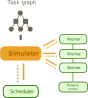
\includegraphics[scale=0.35]{estee/estee-architecture}
	\caption{\estee{} architecture}
	\label{fig:estee-architecture}
\end{figure}

\estee{} provides abstract interfaces for the task scheduler, the worker and the
network model (which simulates network communication and contention). Users can thus easily provide
their own implementations of these interfaces, and in turn override both the behavior of the
scheduler and of the cluster and its network topology.

One of our goals for \estee{} was to make it very easy to write new scheduling
algorithms and make the scheduler approachable for other researchers that might want to experiment
with task schedulers. That was also one of the motivations for deciding to create
\estee{} in Python, which facilitates experimentation. \Autoref{lst:estee-example} shows
an example of a task graph simulation that demonstrates the simplicity of defining a task graph
simulation using \estee{}. The output of the simulation is both the makespan and
also a detailed trace that can be used to visualize the individual task-to-worker assignments and
task execution time spans.

\begin{listing}
	\begin{minted}[fontsize=\normalsize]{python}
# Create task graph containing 3 tasks
# Each task runs for 1s and requires 1 CPU core
#
#     t0
#     | (50MB output)
#    / \
#  t1   t2
tg = TaskGraph()
t0 = tg.new_task(duration=1, cpus=1, output_size=50)
t1 = tg.new_task(duration=1, cpus=1)
t1.add_input(t0)
t2 = tg.new_task(duration=1, cpus=1)
t2.add_input(t0)

# Create a task scheduler
scheduler = BlevelGtScheduler()

# Define cluster with 2 workers (1 CPU core each)
workers = [Worker(cpus=1) for _ in range(2)]

# Define MaxMinFlow network model (100MB/s bandwidth)
netmodel = MaxMinFlowNetModel(bandwidth=100)

# Run simulation, return the estimated makespan in seconds
simulator = Simulator(tg, workers, scheduler, netmodel, trace=True)
makespan = simulator.run()
print(f"Task graph execution makespan = {makespan}s")
    \end{minted}
	\caption{Simple task graph simulation example using \estee{}}
	\label{lst:estee-example}
\end{listing}

\estee{} supports general task graphs represented by a \gls{dag}.
Each task has an associated duration, and can contain multiple outputs (data objects), each with an
associated size. It can also specify how many cores it requires, to model the common requirement of
executing multi-threaded functions and programs on modern \gls{hpc} machines. The
used task graph model corresponds to the task graph definition introduced
in~\Autoref{ch:taskgraphs}.

\subsection{Communication model}
Some previous scheduler surveys assume that the time to transfer a data object from one worker to
another depends merely on the size of the data object, and not on other factors, such as current
network utilization or interference~\cite{tang2010list,yao2013task,wang2018list,kwok1996dynamic}. This is an unrealistic assumption, as
the latency and bandwidth of actual computer networks is affected (among other things) by other
communication happening concurrently on the same network. Moreover, a real worker implementation
would download more than a single data object simultaneously, which further affects the transfer
durations, because the worker's bandwidth will be shared by multiple network transfers. We will use
the term \emph{communication model} and \emph{network model} interchangeably in this chapter.

We provide a more realistic network model that simulates full-duplex communication between workers,
where the total (data object) upload and download bandwidth of each worker is limited. The sharing
of bandwidth between worker connections is modeled by the
\emph{max-min fairness model}~\cite{bertsekas_1992}. Max-min fairness provides a bandwidth allocation
for each worker. If an allocation of any participant is increased, then we decrease the allocation
of some other participant with an equal or smaller allocation. When a data object transfer starts
or finishes, the data flow between workers is recomputed immediately; thus we neglect the fact that
it may take some time for the bandwidth to fully saturate.

This model is not as accurate as e.g.\ packet-level simulation implemented in some other
simulators~\cite{simgrid}, but it is a notable improvement over the naive model and it
provides reasonable runtime performance. To provide a baseline that corresponds to the naive model
described above, which has been used in several previous works, \estee{} also
implements a \emph{simple} network model. The used networking model can be configured
with an arbitrary network bandwidth amount for a given simulation.

\subsection{Scheduler parameters}
\estee{} implements support for two parameters that can affect scheduler
performance, and which we have not seen examined in detail in existing literature:
\begin{description}[wide=0pt]
	\item[\acrlong{msd}] Non-trivial schedulers create task assignments continuously during task graph execution, based on
		the current worker load and task completion times. That means that they are not invoked only once,
		but rather the task runtime invokes them repeatedly to ask them to produce assignments for tasks
		that are (or soon will be) ready to be executed at any given point in time.

		It then becomes important for a task runtime to decide when exactly it should invoke the scheduler.
		It could try to make a scheduling decision every time a task is finished; however, in practice
		there is often an upper bound on the number of scheduler invocations per second. It might be
		introduced artificially, to reduce the scheduling overhead, or it might be caused by a software or
		hardware limitation (e.g.\ messages containing task updates cannot be received more often).
		Furthermore, creating a new schedule after each task status change might not be optimal. The
		runtime can also accumulate changes for a short time period, and then provide the scheduler with a
		batch of status updates. While this increases the latency of task assignments, it can give the
		scheduler more context to work with, when it decides how it should assign tasks to workers.

		To test our hypothesis that the scheduler invocation rate can affect its performance, we introduce
		a parameter called \gls{msd}, which forces a minimal delay between two scheduler
		invocations, i.e.\ the scheduler cannot be invoked again before at least \gls{msd}
		time units have elapsed since its previous invocation.
	\item[Information mode] Many existing task scheduler descriptions assume that the duration of each task (and the size of
		each data object) is known in advance. However, this assumption is very seldom upheld when
		executing real-world task graphs. Tasks are usually specified using arbitrary function or binary
		invocations, and it is difficult to estimate their duration up front. Task runtimes thus have to
		work with completely missing information about task durations, depend on potentially imprecise user
		estimates, or calculate their own estimates based on historical task execution data. Task
		benchmarks usually use simulated task durations, which are provided to the scheduler. However, this
		might not realistically represent the scheduler's behavior for actual task graphs, for which we
		usually do not know task durations precisely before they are executed.

		We use a parameter called \emph{Information mode (imode)}, which controls the amount of knowledge the
		scheduler has of the duration of tasks. It can be set to one of the following values:
		\begin{description}
			\item[exact] The scheduler has access to the exact duration of each task and the exact size of each data object
				in the whole task graph.
			\item[user] The scheduler has access to user-defined estimations for each task in the task graph. These
				estimations are sampled from a random distribution that corresponds to a specific kind of task
				within the workflow. For example, in a task graph that performs three kinds of tasks (e.g.\
				preprocessing, computation and postprocessing), each kind of task would have its own distribution.
				We have categorized the tasks of task graphs that we have used for scheduler benchmarks described
				in~\Autoref{sec:estee-benchmarks} manually, to simulate a user that has some knowledge of the task graph
				that they are trying to compute and is able to provide some estimate of task durations and data
				object sizes.
			\item[mean] The scheduler only has access to the mean duration of all tasks and the mean size of all data
				objects in the executed task graph. This simulates a situation where a similar task graph is
				executed repeatedly, and thus there is at least some aggregated information about the task
				properties available from an earlier run.
		\end{description}
		Another possible mode to consider could be to not provide the scheduler with any task durations nor
		data object sizes in advance. This behavior would in fact correspond closely to a real-world
		execution of a task graph, where we usually do not know these task properties a priori. However, it
		is challenging to use this approach when benchmarking schedulers. Scheduler implementations are
		typically described with the assumption that task durations are known, and the scheduling
		algorithms are often fundamentally based on calculations that make use of them.

		If we took away this information, some schedulers would not be able to function, as their behavior
		is strongly influenced by an estimate of the duration of each task. Therefore, we propose using the
		\emph{mean} mode instead of not providing the scheduler with any information. We assume
		that even if the scheduler knows nothing in advance, it could always gradually record the durations
		and sizes of finished tasks, and these values would eventually converge to the global mean. In
		practice, this would take some time, while in our environment the schedulers know about the mean in
		advance. Nevertheless, as was already mentioned, we can often get a reasonable estimate of the mean
		durations based on previous executions of similar workflows.
\end{description}

%\subsection{Worker inner scheduler}
%Since each worker has to keep track of its running tasks, manage resources, and
%handle data object transfers, it becomes relatively complex. In practice, the global
%scheduler cannot micromanage each worker because this approach could not scale
%to a larger number of workers. Therefore, we model a situation where each
%worker has its own inner scheduler. We call it \emph{w-scheduler} and we
%reserve the word ``scheduler'' for the global scheduler that assigns tasks to
%workers.
%
%The w-scheduler is not a subject of study in this work, hence we are going to
%fix one particular worker scheduler and execute all experiments with it.
%The implementation is inspired by the worker implementation used in
%HyperLoom~\citep{hyperloom} and Rain. It is described in Appendix~A.

\subsection{Schedulers}
\label{subsec:estee-schedulers}
There are many task scheduling approaches, and an enormous number of various task scheduling
algorithms. We have implemented a set of task schedulers that are representatives of several common
scheduling approaches, inspired by a list of schedulers from a survey performed by Wang and
Sinnen~\cite{wang2018list}. We have included several representatives of the simplest and
perhaps most common scheduling approach, called list-scheduling, where the scheduler sorts tasks
based on some priority criteria, and then repeatedly chooses the task with the highest priority and
assigns it to a worker, which is selected by some heuristic. In addition to list-scheduling, we
have also implemented more complex approaches, such as schedulers that use work-stealing or genetic
algorithms.

Below is a list of schedulers that we have implemented and benchmarked\footnote{The labels of the individual schedulers correspond to labels used in charts that will be presented
in~\Autoref{sec:estee-benchmarks}.}:

\begin{description}[wide=0pt,itemsep=0pt,topsep=4pt]
	\item[blevel] \gls{hlfet}~\cite{hlfet1974} is a
		foundational list-based scheduling algorithm that prioritizes tasks based on their
		\emph{b-level}. B-level of a task is the length of the longest path from the task to any
		leaf task (in our case the length of the path is computed using durations of tasks, without taking
		data object sizes into account). The tasks are scheduled in a decreasing order based on their
		b-level.

	\item[tlevel]
		Smallest Co-levels First with Estimated Times~\cite{kwok1999static} is similar to
		\gls{hlfet}, with the exception that the priority value computed for each task (which is
		called \emph{t-level} here) is computed as the length of the longest path from any source
		task to the given task. This value corresponds to the earliest time that the task can start. The
		tasks are scheduled in an increasing order based on their t-level.

	\item[dls]
		Dynamic Level Scheduling~\cite{sih1993compile} calculates a dynamic level for each task-worker
		pair. It is equal to the static b-level lessened by the earliest time that the task can start on a
		given worker (considering necessary data transfers). In each scheduling step, the task-worker pair
		that maximizes this value is selected.

	\item[mcp]
		The Modified Critical Path~\cite{wu1990hypertool} scheduler calculates the ALAP
		(as-late-as-possible) time for each task. This corresponds to the latest time the task can start
		without increasing the total schedule makespan. The tasks are then ordered in ascending order based
		on this value, and scheduled to the worker that allows their earliest execution.

	\item[etf]
		The ETF (Earliest Time First) scheduler~\cite{hwang1989scheduling} selects the task-worker pair that
		can start at the earliest time at each scheduling step. Ties are broken by a higher b-level
		precomputed at the start of task graph execution.

	\item[genetic]
		This scheduler uses a genetic algorithm to schedule tasks to workers, using the mutation and
		crossover operators described in~\cite{omara2009genetic}. Only valid schedules are considered; if no
		valid schedule can be found within a reasonable number of iterations, a random schedule is
		generated instead.

	\item[ws]
		This is an implementation of a simple work-stealing algorithm. The default policy is that each task
		that is ready to be executed (all its dependencies are already computed) is always assigned to a
		worker where it can be started with a minimal transfer cost. The scheduler then continuously
		monitors the load of workers. When a worker starts to starve (and thus does not have enough tasks
		to compute), a portion of tasks assigned to other workers is rescheduled to the starving worker.
\end{description}

In addition to these schedulers, we have also implemented several naive schedulers, which serve as
a baseline for scheduler comparisons.

\begin{description}[wide=0pt]
	\item[single]
		This scheduler simply assigns all tasks to a single worker (it selects the worker with the most
		cores). The resulting schedule never induces any data transfers between workers, and does not take
		advantage of any parallelism between workers.
	\item[random]
		This scheduler simply assigns each task to a random worker using a \gls{prng} engine.
\end{description}

We have strived to implement the mentioned list-based schedulers (\emph{blevel},
\emph{tlevel}, \emph{dls}, \emph{mcp}, \emph{etf})
as closely as possible to their original description. These list-based algorithms mostly focus on
selecting the next task to schedule, but an important question (that comes up during their
implementation) is to what worker should the selected task be scheduled. The algorithm descriptions
often mention assigning the task to a worker that allows the earliest start time of the task. While
that is surely a reasonable heuristic, it is not clear how exactly such a worker should be found,
because the exact earliest start time often cannot be determined precisely in advance, since its
calculation might encompass network transfers whose duration is uncertain. This seemingly simple
implementation detail is crucial for implementing the scheduler, and it should thus be included in
the description of all scheduling algorithms that make use of such a heuristic.

\estee{} implementations of these schedulers use a simple estimation of the earliest
start time, which is based on the currently executing and already scheduled tasks of a worker and
an estimated network transfer cost based on uncontented network bandwidth (the
\emph{simple} network model is used for the scheduler's estimation of the network
transfer cost).

In order to test our hypothesis that the worker selection approach is important and affects the
scheduler's behavior, we have also created extended versions of the \emph{blevel},
\emph{tlevel} and \emph{mcp} schedulers. These modified versions use a
worker selection heuristic called ``greedy transfer``. We have not applied this heuristic to other
list-based schedulers, because it would fundamentally change their behavior.

The greedy transfer heuristic assigns the selected task to a worker that has a sufficient number of
free cores on which the task may be executed, and that requires the minimal data transfer (sum over
all sizes of data objects that have to be transferred to that worker). It also adds support for
clusters where some machines have a different number of cores than others. When a task
$t$ that needs $c$ cores cannot be scheduled because of an
insufficient number of free cores, the list-scheduling continues by taking another task in the list
instead of waiting for more free cores. This task will only consider workers that have fewer than
$c$ cores. This allows for scheduling more tasks while it does not modify the
priority of tasks because $t$ cannot be scheduled on such workers anyway. Note
that when all workers have the same number of cores, the behavior is identical to ordinary
list-scheduling.

\subsection{Task graphs}
To facilitate task scheduler experiments, \estee{} contains a task graph generator
that is able to generate parametrized instances of various categories of task graphs. Graphs from
each category can be generated using several parameters that affect their resulting size and shape.
To increase the variability of the graphs, properties like task durations or data object sizes are
sampled from a normal distribution. Below is a description of the three categories of task graphs
that can be generated:

\begin{description}[wide=0pt,itemsep=0pt,topsep=4pt]
	\item[elementary] This category contains trivial graph shapes, such as tasks with no dependencies or simple
		``fork-join'' graphs. These graphs can test the behavior of scheduler heuristics on basic task
		graph building blocks that frequently form parts of larger workflows. Examples of these graphs can
		be found in~\Autoref{app:benchmarks} (\Autoref{fig:estee-elementary-shapes}).

	\item[irw] This generator creates graphs that are inspired by real-world task graphs, such as machine-learning
		cross-validations or map-reduce workflows.

	\item[pegasus] This category is derived from graphs created by the Synthetic Workflow
		Generators~\cite{pegasusgraphs}. The generated graphs correspond to the \emph{montage},
		\emph{cybershake}, \emph{epigenomics}, \emph{ligo} and \emph{sipht}
		Pegasus workflows. The graphs have been extended with additional properties required for testing
		information modes (notably expected task durations and data object sizes for the
		\emph{user} information mode).
\end{description}

\section{Task scheduler evaluation}
\label{sec:estee-benchmarks}
We have carried out an extensive analysis of the performance of several task scheduling algorithms
on various task graphs using the \estee{} simulator. The aim of the analysis was to
explore the behavior of various schedulers in a complex simulation environment. In addition to
comparing the schedulers among each other, we also wanted to test how their performance differs
between various communication models and scheduler parameters.

Note that since the used simulation environment is focused on simulating different task graph
schedules and network transfers, and it does not model the actual execution of the scheduler nor
the task runtime in a cycle-accurate way, the term \emph{scheduler performance} refers to the simulated
makespan of task graphs executed using schedules provided by the given scheduler. In other words,
our experiments estimate how quickly a given task graph would be fully computed on a cluster, using
a given network model, while being scheduled by a specific scheduling algorithm.

\subsection{Benchmark configuration}
Below, you can find descriptions of the cluster, scheduler and task graph configurations that we
have used for our benchmarks.

\begin{description}[wide=0pt,itemsep=0pt,topsep=4pt]
	\item[Task graphs] The \estee{} graph generators were used to generate a collection of task graphs that
		were used in the benchmarks. The properties of all used graphs are summarized
		in~\Autoref{app:benchmarks} (\Autoref{tab:estee-graph-properties}). The generated task graph dataset is available as a reproducible
		artifact~\cite{estee_graphs}.
	\item[Schedulers] We have benchmarked all schedulers described in~\Autoref{subsec:estee-schedulers}. Schedulers that use the
		greedy transfer heuristic are labeled in the benchmark results with a \emph{-gt}
		suffix.
	\item[Scheduler parameters] To evaluate the effect of minimal scheduling delay, we have used a baseline value of zero, where
		the scheduler is invoked immediately after any task status update, and then a delay of
		$0.1$, $0.4$, $1.6$ and $6.4$
		seconds. In the cases where \gls{msd} is non-zero, we have also added a
		$50$ milliseconds delay before sending the scheduler decision to workers, to
		simulate the time taken by the scheduler to produce the schedule. For experiments that do not focus
		on \gls{msd}, we always use an \gls{msd} of $0.1$ seconds
		and the $50$ milliseconds computation delay. To evaluate information modes, we
		have used the \emph{exact}, \emph{user} and \emph{mean} imodes. For
		experiments that do not focus on imodes, we always use the \emph{exact} mode.
	\item[Network models] The simple (labeled \emph{simple}) and max-min (labeled \emph{max-min}) network
		models were used, with bandwidth speeds ranging from \SI{32}{\mebi\byte}/s to
		\SI{8}{\gibi\byte}/s. For experiments that do not focus on the network model (e.g.\ when imodes
		are being compared), we always use the \emph{max-min} network model.
	\item[Clusters] We have used the following five cluster (worker) configurations (where $w \times c$ means
		that the cluster has $w$ workers and each worker has $c$
		cores):  8$\times$4, 16$\times$4, 32$\times$4,
		16$\times$8, 32$\times$16.
\end{description}

\subsection{Evaluation}
This section discusses selected results of the described benchmarks. Complete benchmark results and
overview charts can be found in~\cite{estee}. The benchmarking environment, input task
graph datasets, all benchmark configurations, results and charts are also freely available as
reproducible artifacts~\cite{estee_results} for further examination.

The benchmarks were executed on the clusters of the IT4Innovations supercomputing
center~\cite{it4i}. The actual characteristics of the cluster hardware is not
important, because all benchmarks were executed using the \estee{} simulator, so the
benchmark results do not depend on the used hardware. Each benchmark that was non-deterministic in
any way (e.g.\ because it used a pseudo-random number generator) was executed twenty times. Unless
otherwise specified, the individual experiments were performed with the default benchmark
configuration that uses the \emph{max-min} network model, the \emph{exact}
information mode and a \acrlong{msd} of \SI{0.1}{\second}.

Note that the vertical axis of some charts presented in this section does not start at zero, as the
goal was to focus on the relative difference between different scheduling algorithms rather than on
the absolute makespan durations.

\subsubsection*{Random scheduler}

\begin{figure}
	\centering
	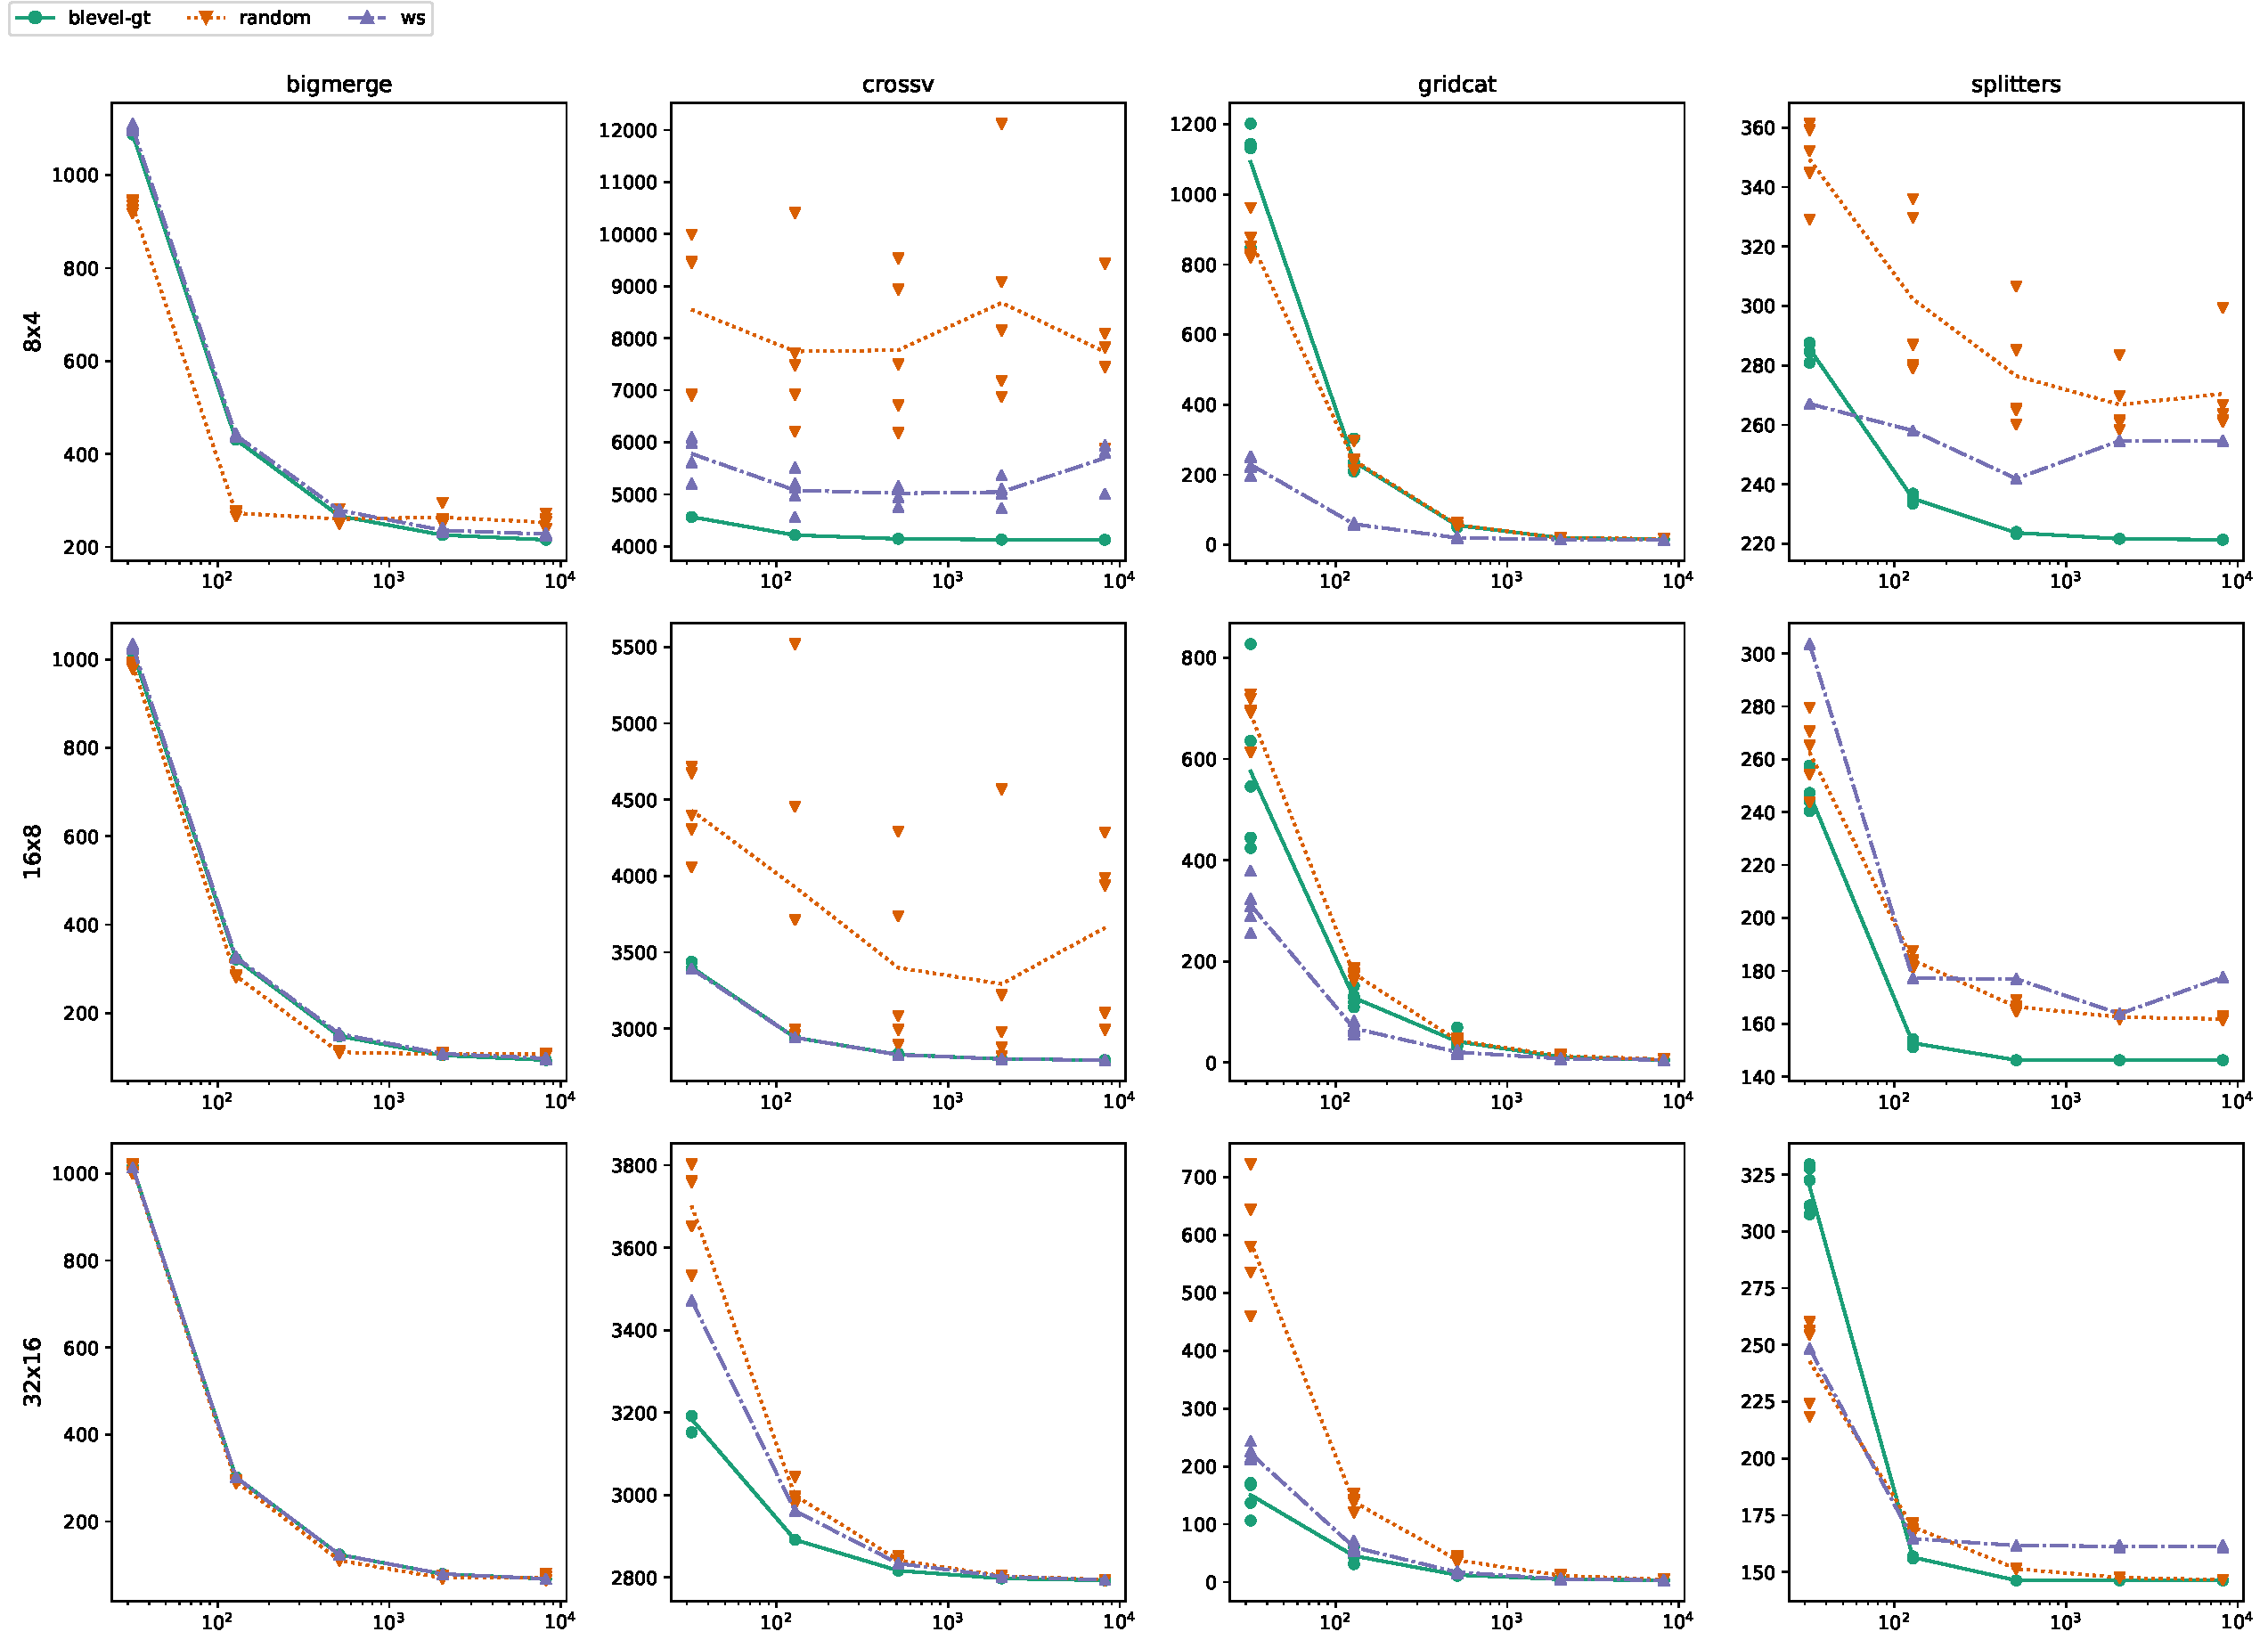
\includegraphics[width=\textwidth]{imgs/estee/charts/random-scheduler}\\
	{\small horizontal axis: bandwidth [MiB/s]; vertical axis: makespan [s]; row: cluster}
	\caption{Performance of the \emph{random} scheduler}
	\label{fig:estee-chart-random-scheduler}
\end{figure}

Given the fact that task scheduling is an NP-hard problem, it would seem that a random scheduling
approach should produce unsatisfying results. Therefore, we wanted to examine how a completely random
scheduler holds up against more sophisticated approaches. \Autoref{fig:estee-chart-random-scheduler} compares the
simulated makespan durations of the \emph{random} scheduler vs. two other competitive
schedulers (\emph{blevel-gt} and the work-stealing \emph{ws} scheduler) on
several task graphs.

While there are indeed cases where random scheduling falls short (for example on the
cross-validation \emph{crossv} task graph, or in situations with many workers and a slow
network), in most cases its performance is similar to other schedulers, and in a few situations it
even surpasses them. Its performance improves with increasing worker count and network speed. This
makes intuitive sense, because if there are enough workers and the network is fast enough to
overcome the cost of exchanging many data objects between them, the specific assignment of tasks
between workers becomes less important. As long as the scheduler is able to keep the workers busy
(which can be ensured even by a random schedule for some task graphs), then the resulting
performance might be reasonable.

We have been able to validate these results in~\cite{rsds}, where we have shown that as
the worker count becomes larger, scheduling decisions can in some cases become less important, and
other factors (like the overhead of the task runtime) might start to dominate the overall task
graph execution cost. This will be described in more detail in~\Autoref{ch:rsds}.

\subsubsection*{Worker selection strategy}

\begin{figure}
	\centering
	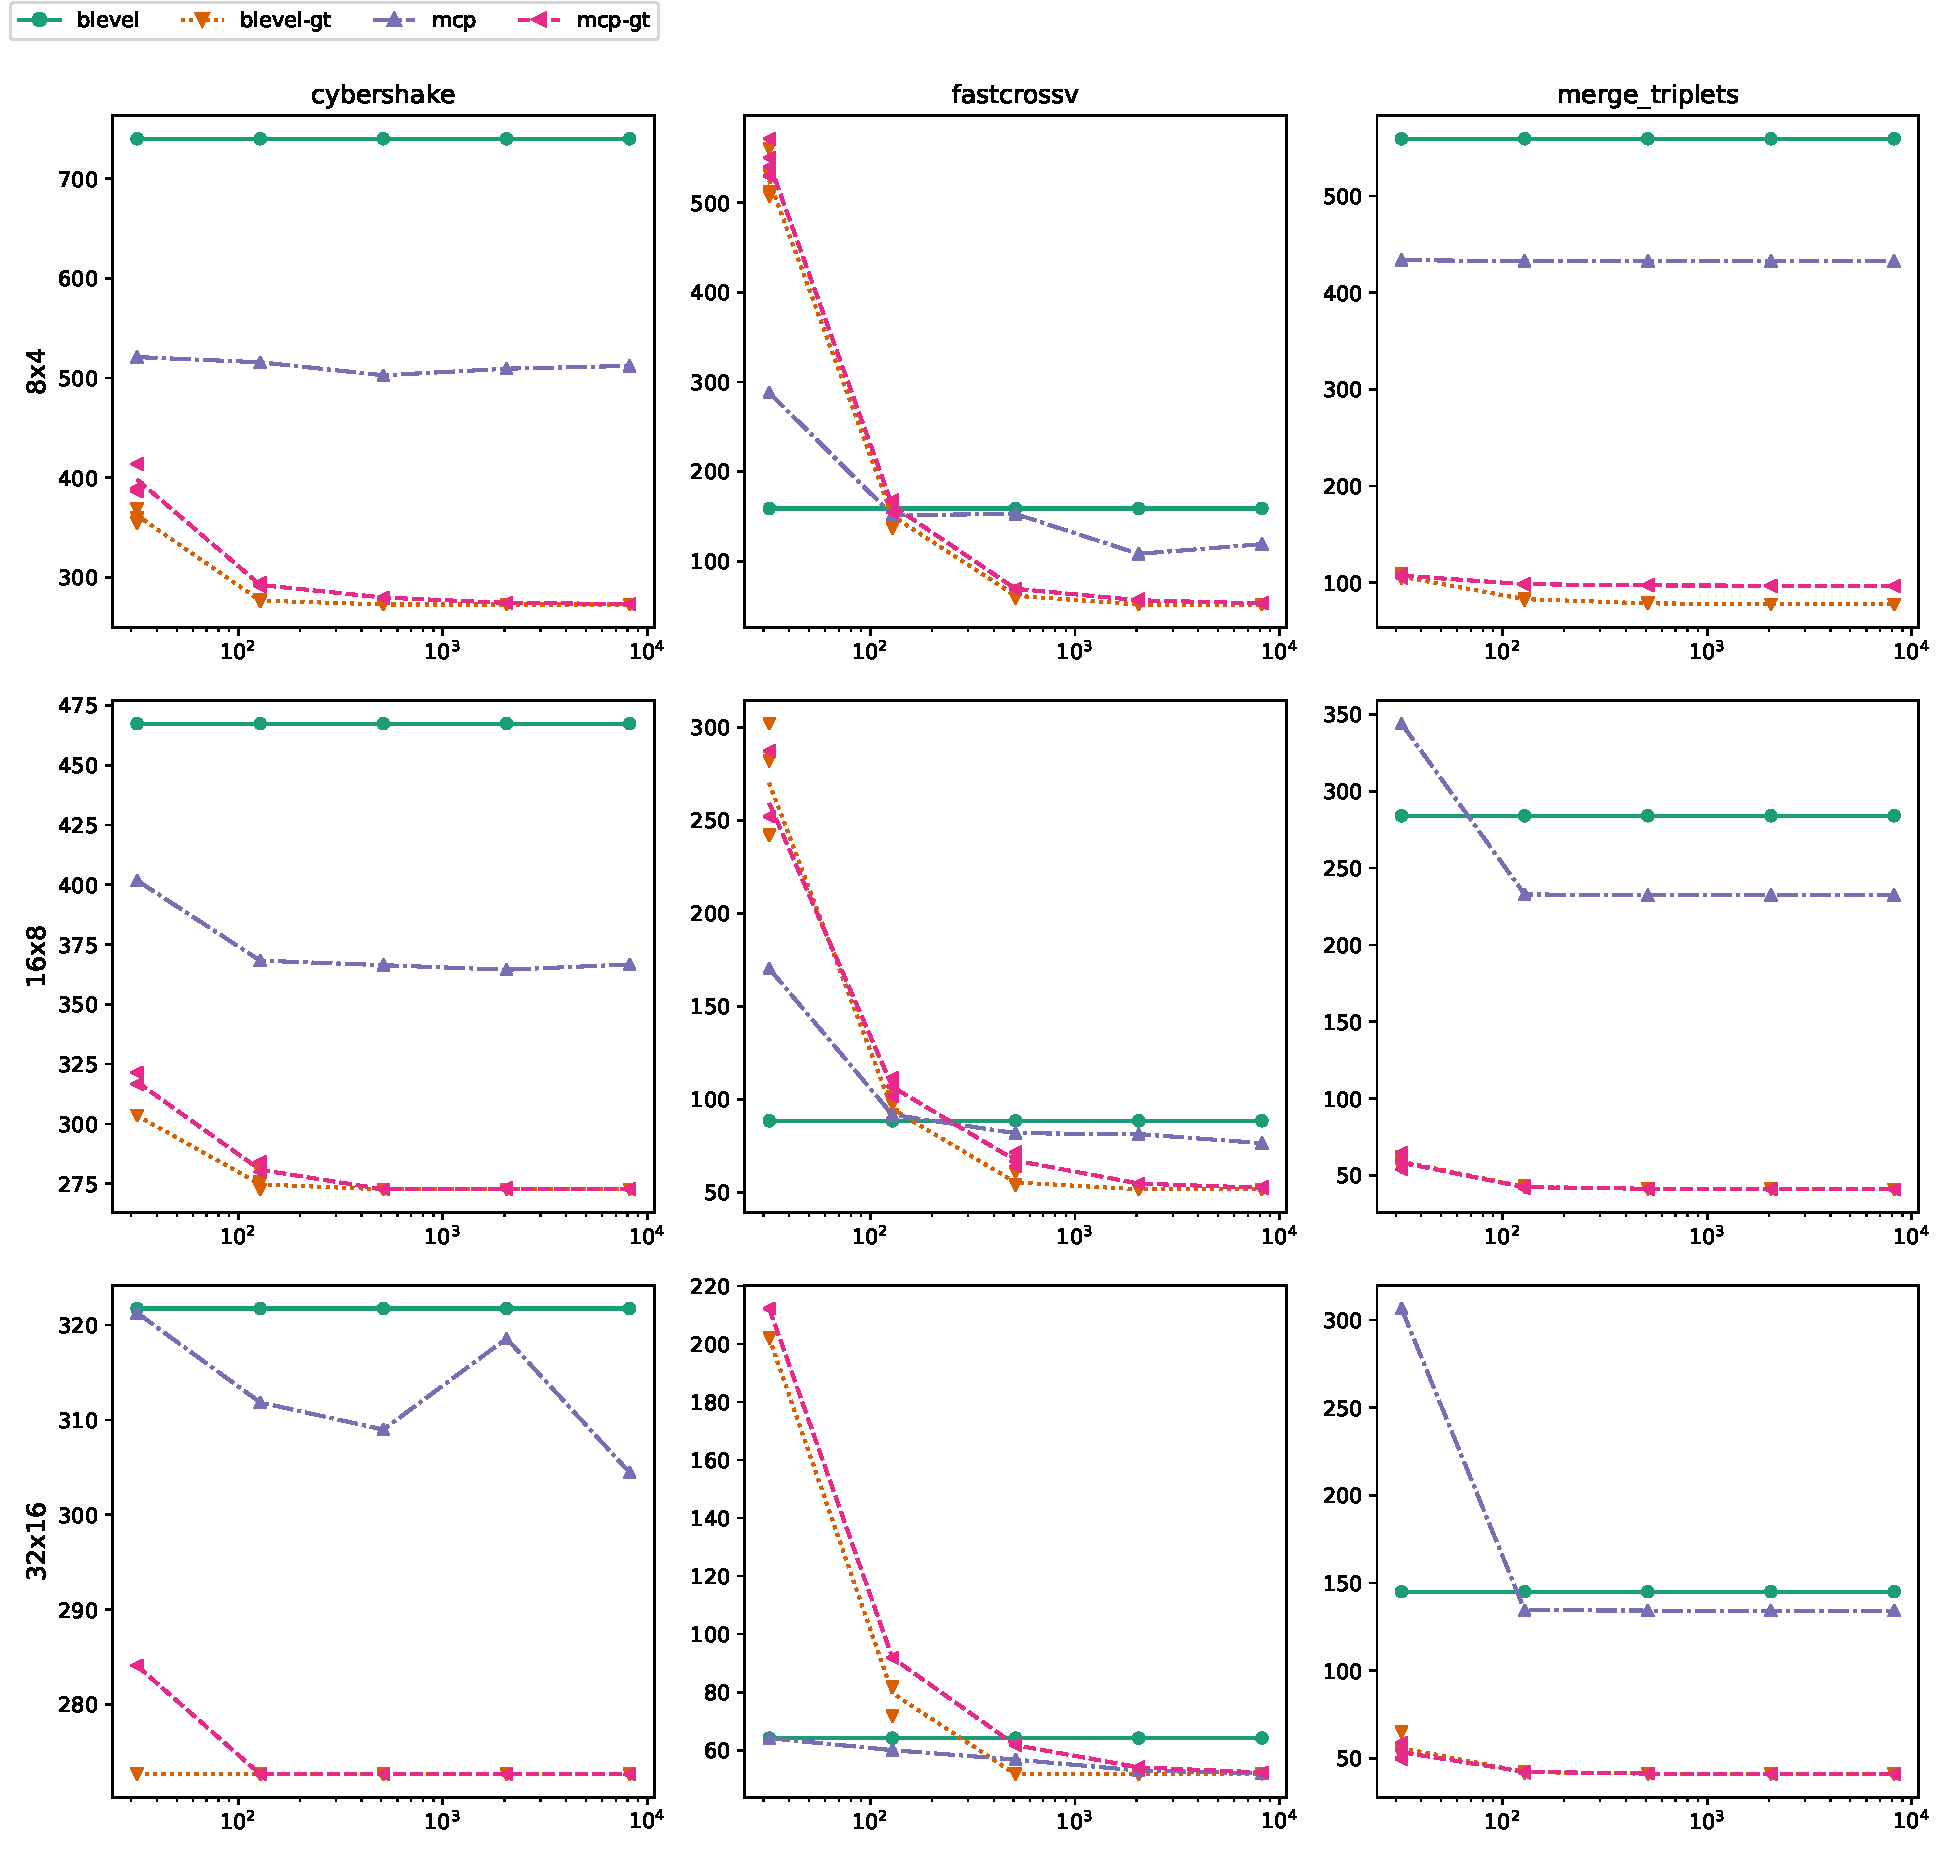
\includegraphics[width=0.8\textwidth]{imgs/estee/charts/gt-scheduler}\\
	{\small horizontal axis: bandwidth [MiB/s]; vertical axis: makespan [s]; row: cluster}
	\caption{Comparison of worker selection strategy}
	\label{fig:estee-chart-gt-scheduler}
\end{figure}

As was explained in~\Autoref{subsec:estee-schedulers}, the descriptions of several schedulers that we have
implemented in~\estee{} do not specify the concrete strategy for selecting a worker
that can start executing a given task as soon as possible. Yet, as we can see
in~\Autoref{fig:estee-chart-gt-scheduler}, this implementation detail is crucial. This chart shows the performance
of two scheduling algorithms (\emph{blevel} and \emph{mcp}), each in two
variants, with the simple selection strategy and with the greedy transfer strategy (the used worker
selection strategy was the only difference between the simple and the \emph{-gt}
suffixed variants).

It can be seen that there is a large difference between these two strategies. In fact, the results
suggest that in these specific scenarios, the worker selection strategy had a larger effect on the
overall performance than the used scheduling (task selection) algorithm, as the variants using
greedy transfer were highly correlated. This suggests that the used worker selection strategy is an
important detail of list-scheduling algorithms that should not be omitted from their descriptions.

\subsubsection*{Network models}

\begin{figure}
	\centering
	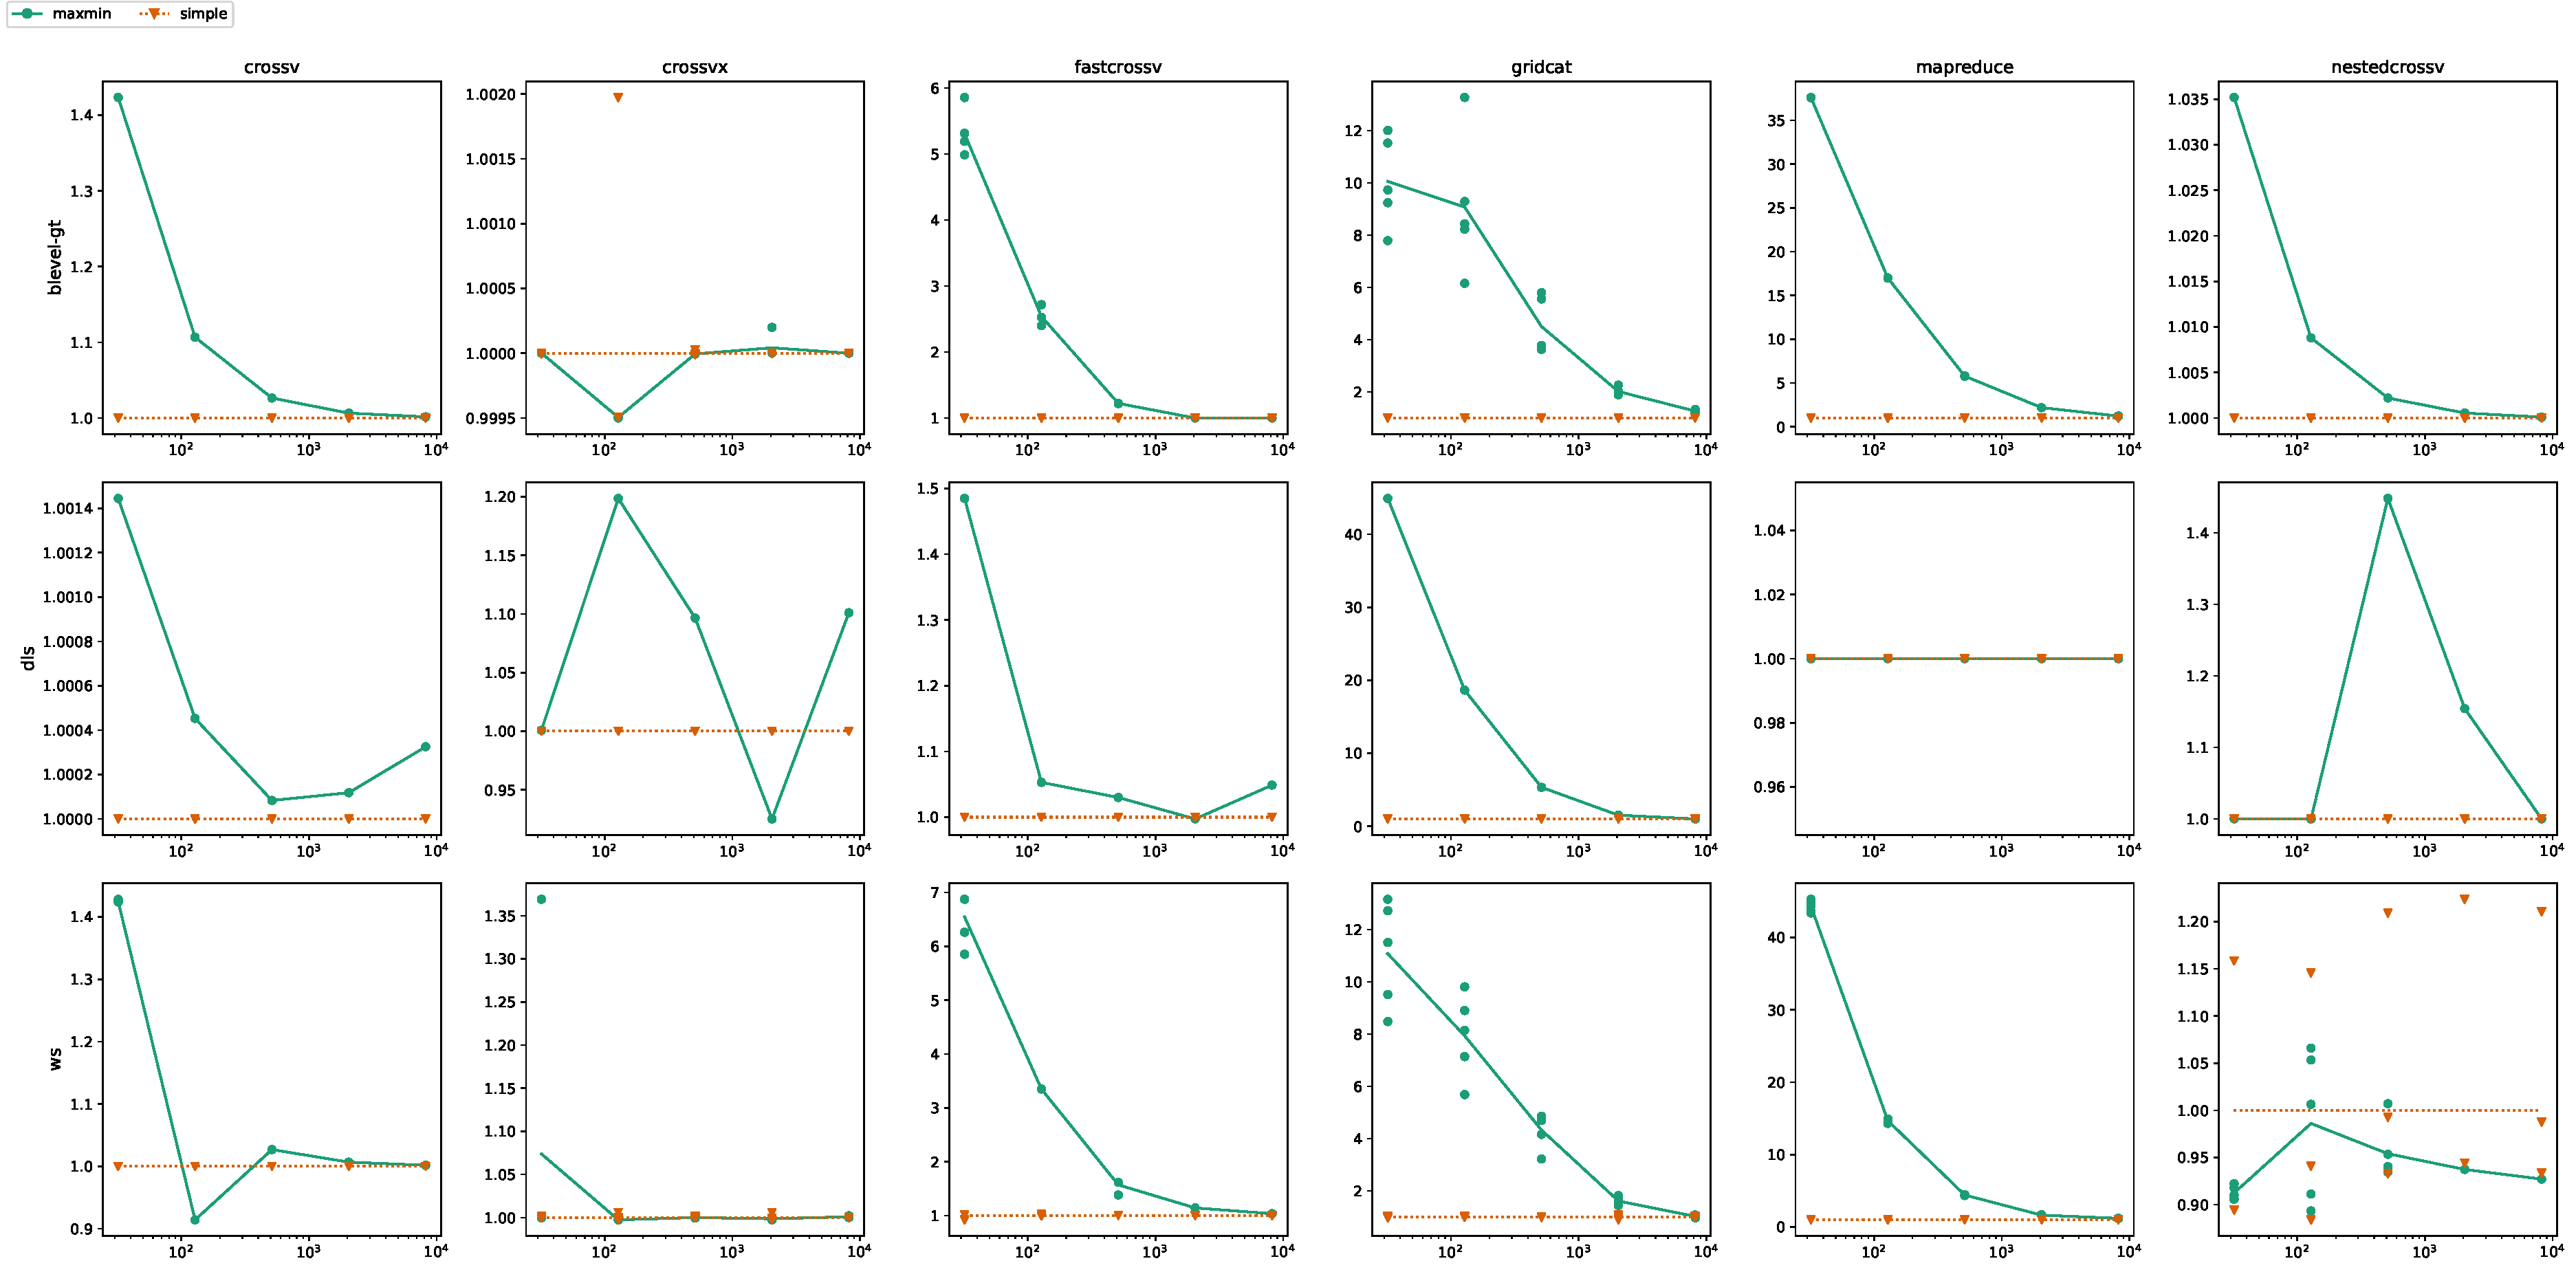
\includegraphics[width=\textwidth]{imgs/estee/charts/irw-32x4-netmodel-score}\\
	{\small horizontal axis: bandwidth [MiB/s]; vertical axis: makespan normalized to average
	of the \emph{simple} model; row: scheduler; cluster $32x4$}
	\caption{Comparison of \emph{max-min} and \emph{simple} network models
	(\emph{irw} dataset)} \label{fig:estee-chart-irw-netmodel}
\end{figure}

%\begin{figure}
%	\centering
%	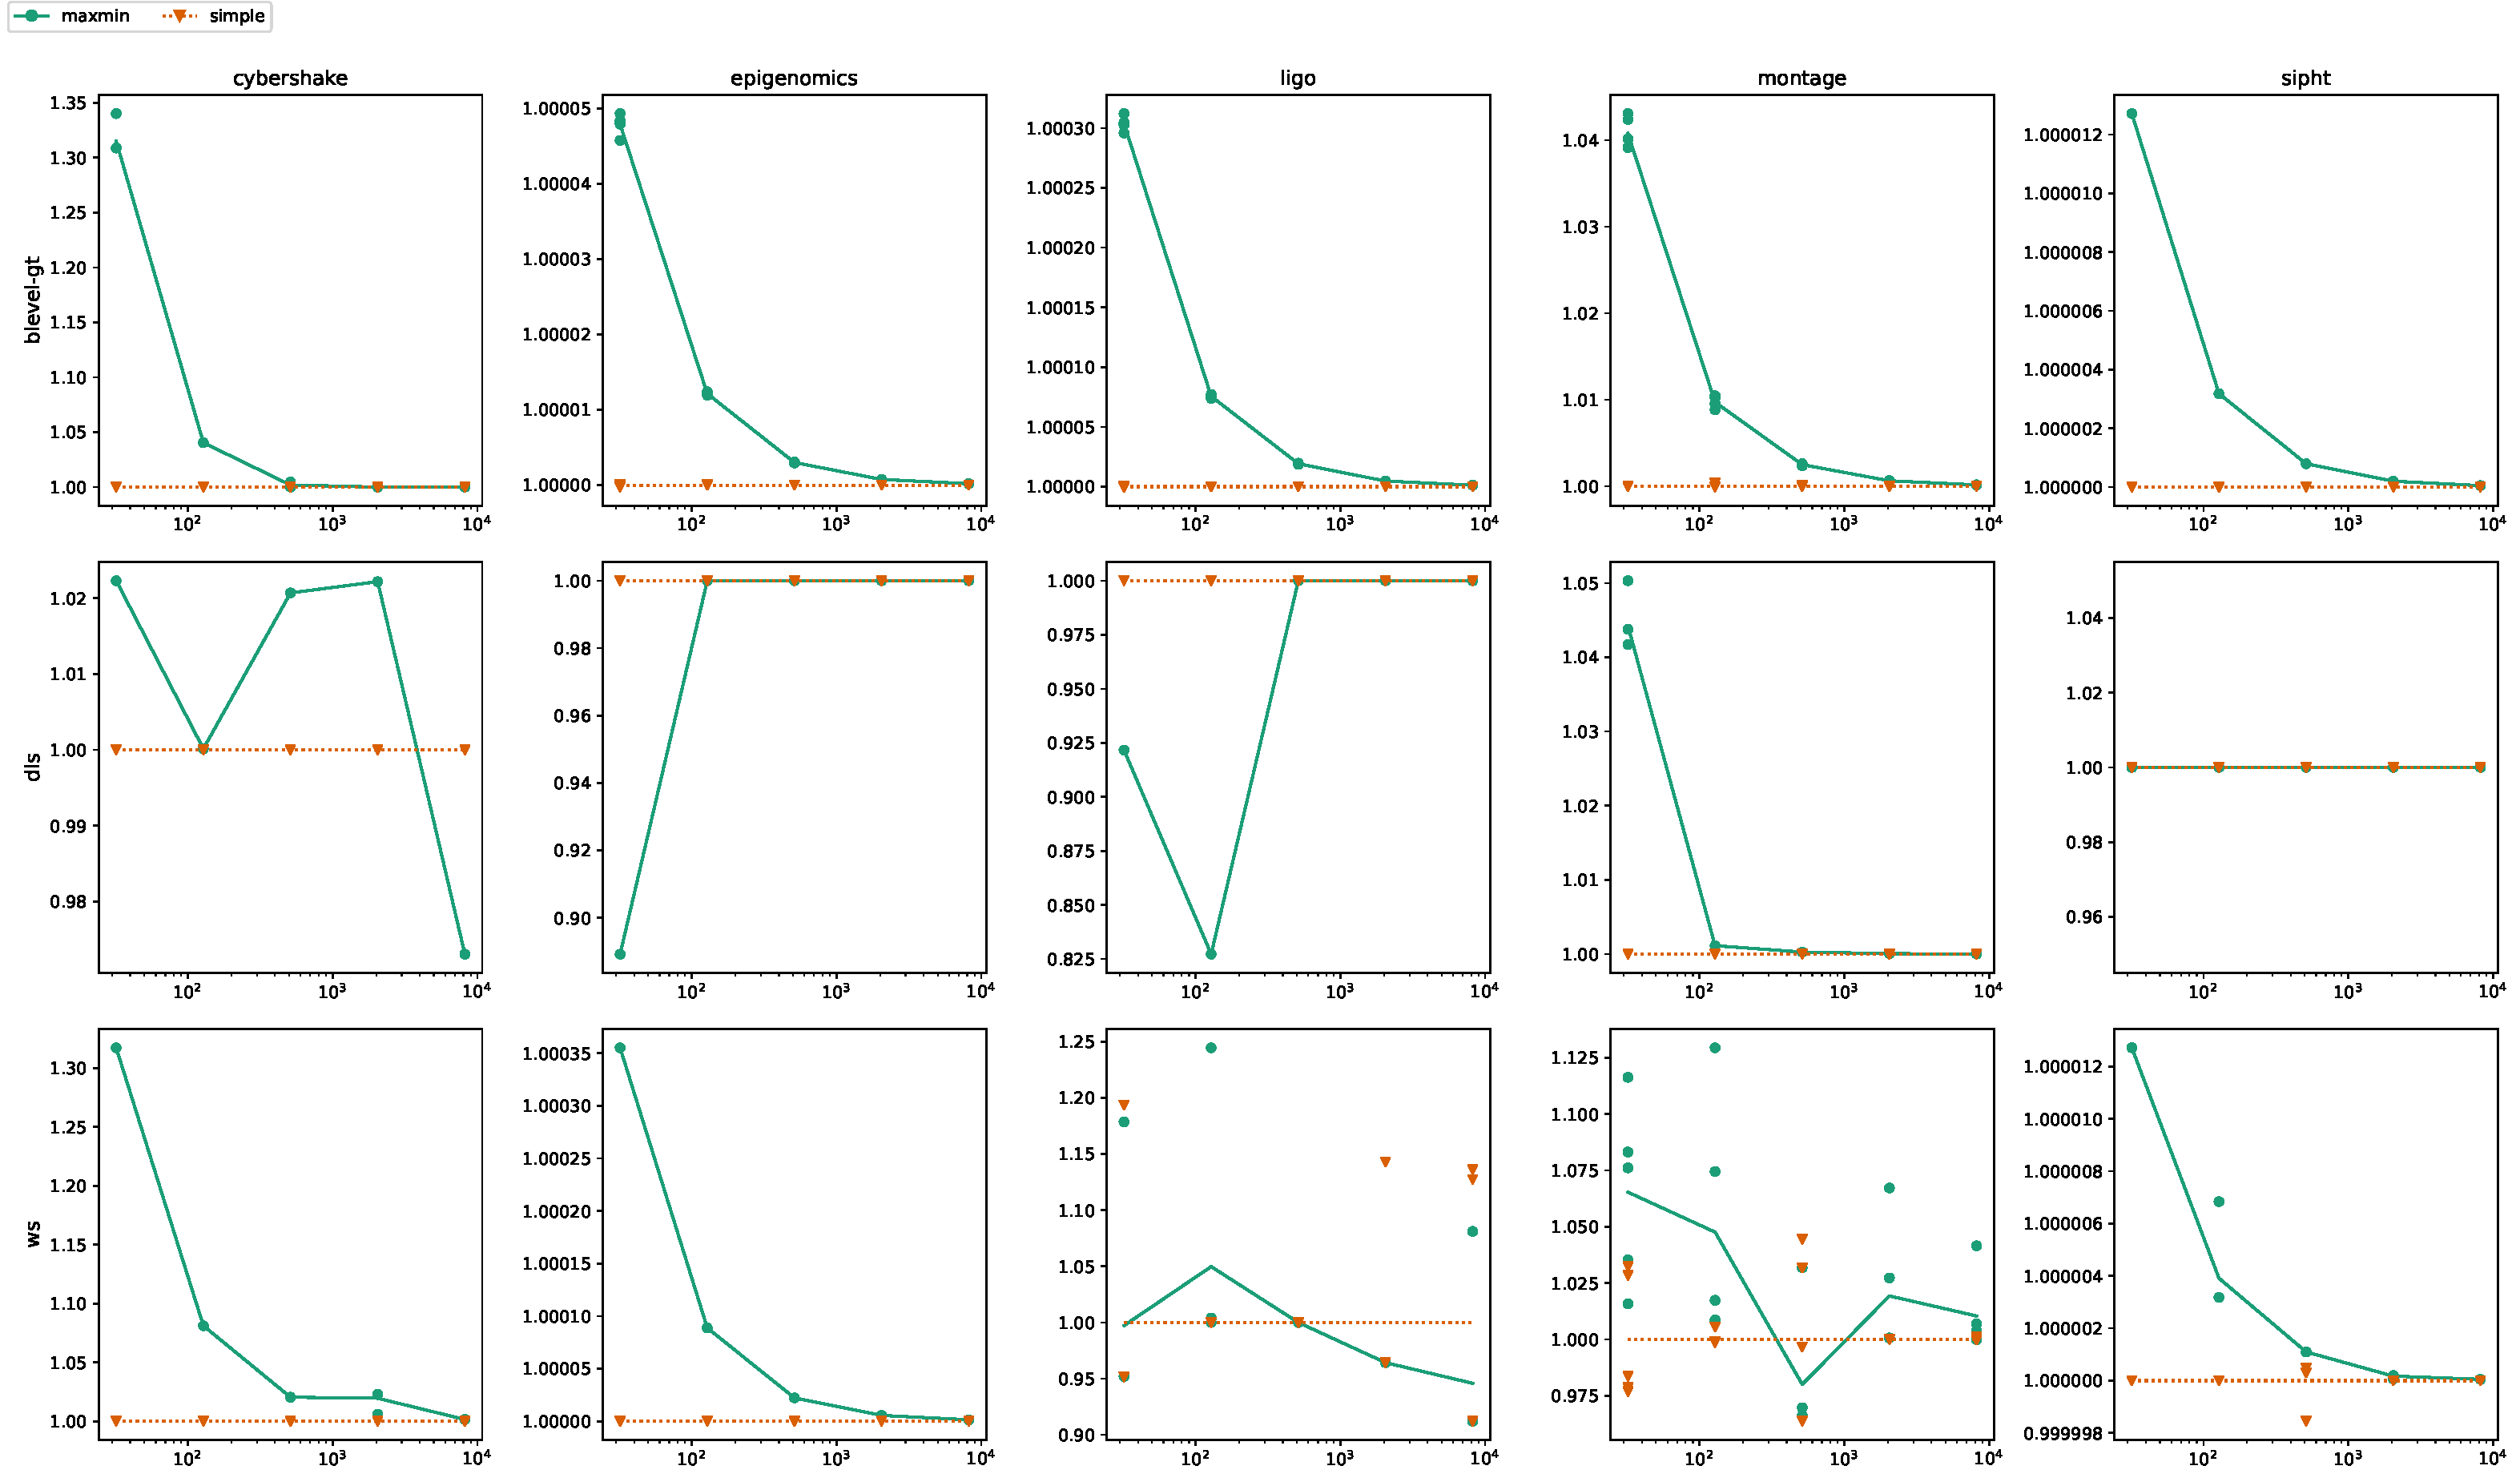
\includegraphics[width=\textwidth]{imgs/estee/charts/pegasus-32x4-netmodel-score}
%	\\ {\small horizontal axis: bandwidth [MiB/s]; vertical axis: execution makespan normalized
%	to average of the \emph{simple} model; row: scheduler, cluster
%	$32x4$} \caption{Comparison of \emph{maxmin} and \emph{simple} network models
%	(\emph{pegasus} dataset)} \label{fig:estee-chart-pegasus-netmodel}
%\end{figure}

\Autoref{fig:estee-chart-irw-netmodel} demonstrates how the used network model affects simulated task
graph makespans for a selected set of task graphs and schedulers, using task graphs from the
\emph{irw} dataset on the $32x4$ cluster with 32 workers. The Y axis
is normalized with respect to the average makespan of simulations performed with the
\emph{simple} network model.

It is clear that especially for slower network bandwidths, the naive \emph{simple} model
often underestimates the resulting makespan. This is caused by the fact that it does not take
network contention into account at all, which causes the overall network transfer duration
estimation to be overly optimistic. As network bandwidth goes up, the difference is reduced, since
there is less overall contention and the transfers are faster in general.

The makespans of simulations with these two network models are sometimes up to an order of
magnitude apart. This is quite significant, because the difference between the performance of
schedulers (with a fixed network model) is otherwise usually within a factor of two, which was
demonstrated both in~\cite{wang2018list} and by results of our other experiments. The gap
between the two network models depends heavily on the used task graph.
 %the difference was much smaller, as can be seen in~\Autoref{fig:estee-chart-pegasus-netmodel}.%For task graphs from the Pegasus dataset,

\subsubsection*{\acrlong{msd}}

\begin{figure}
	\centering
	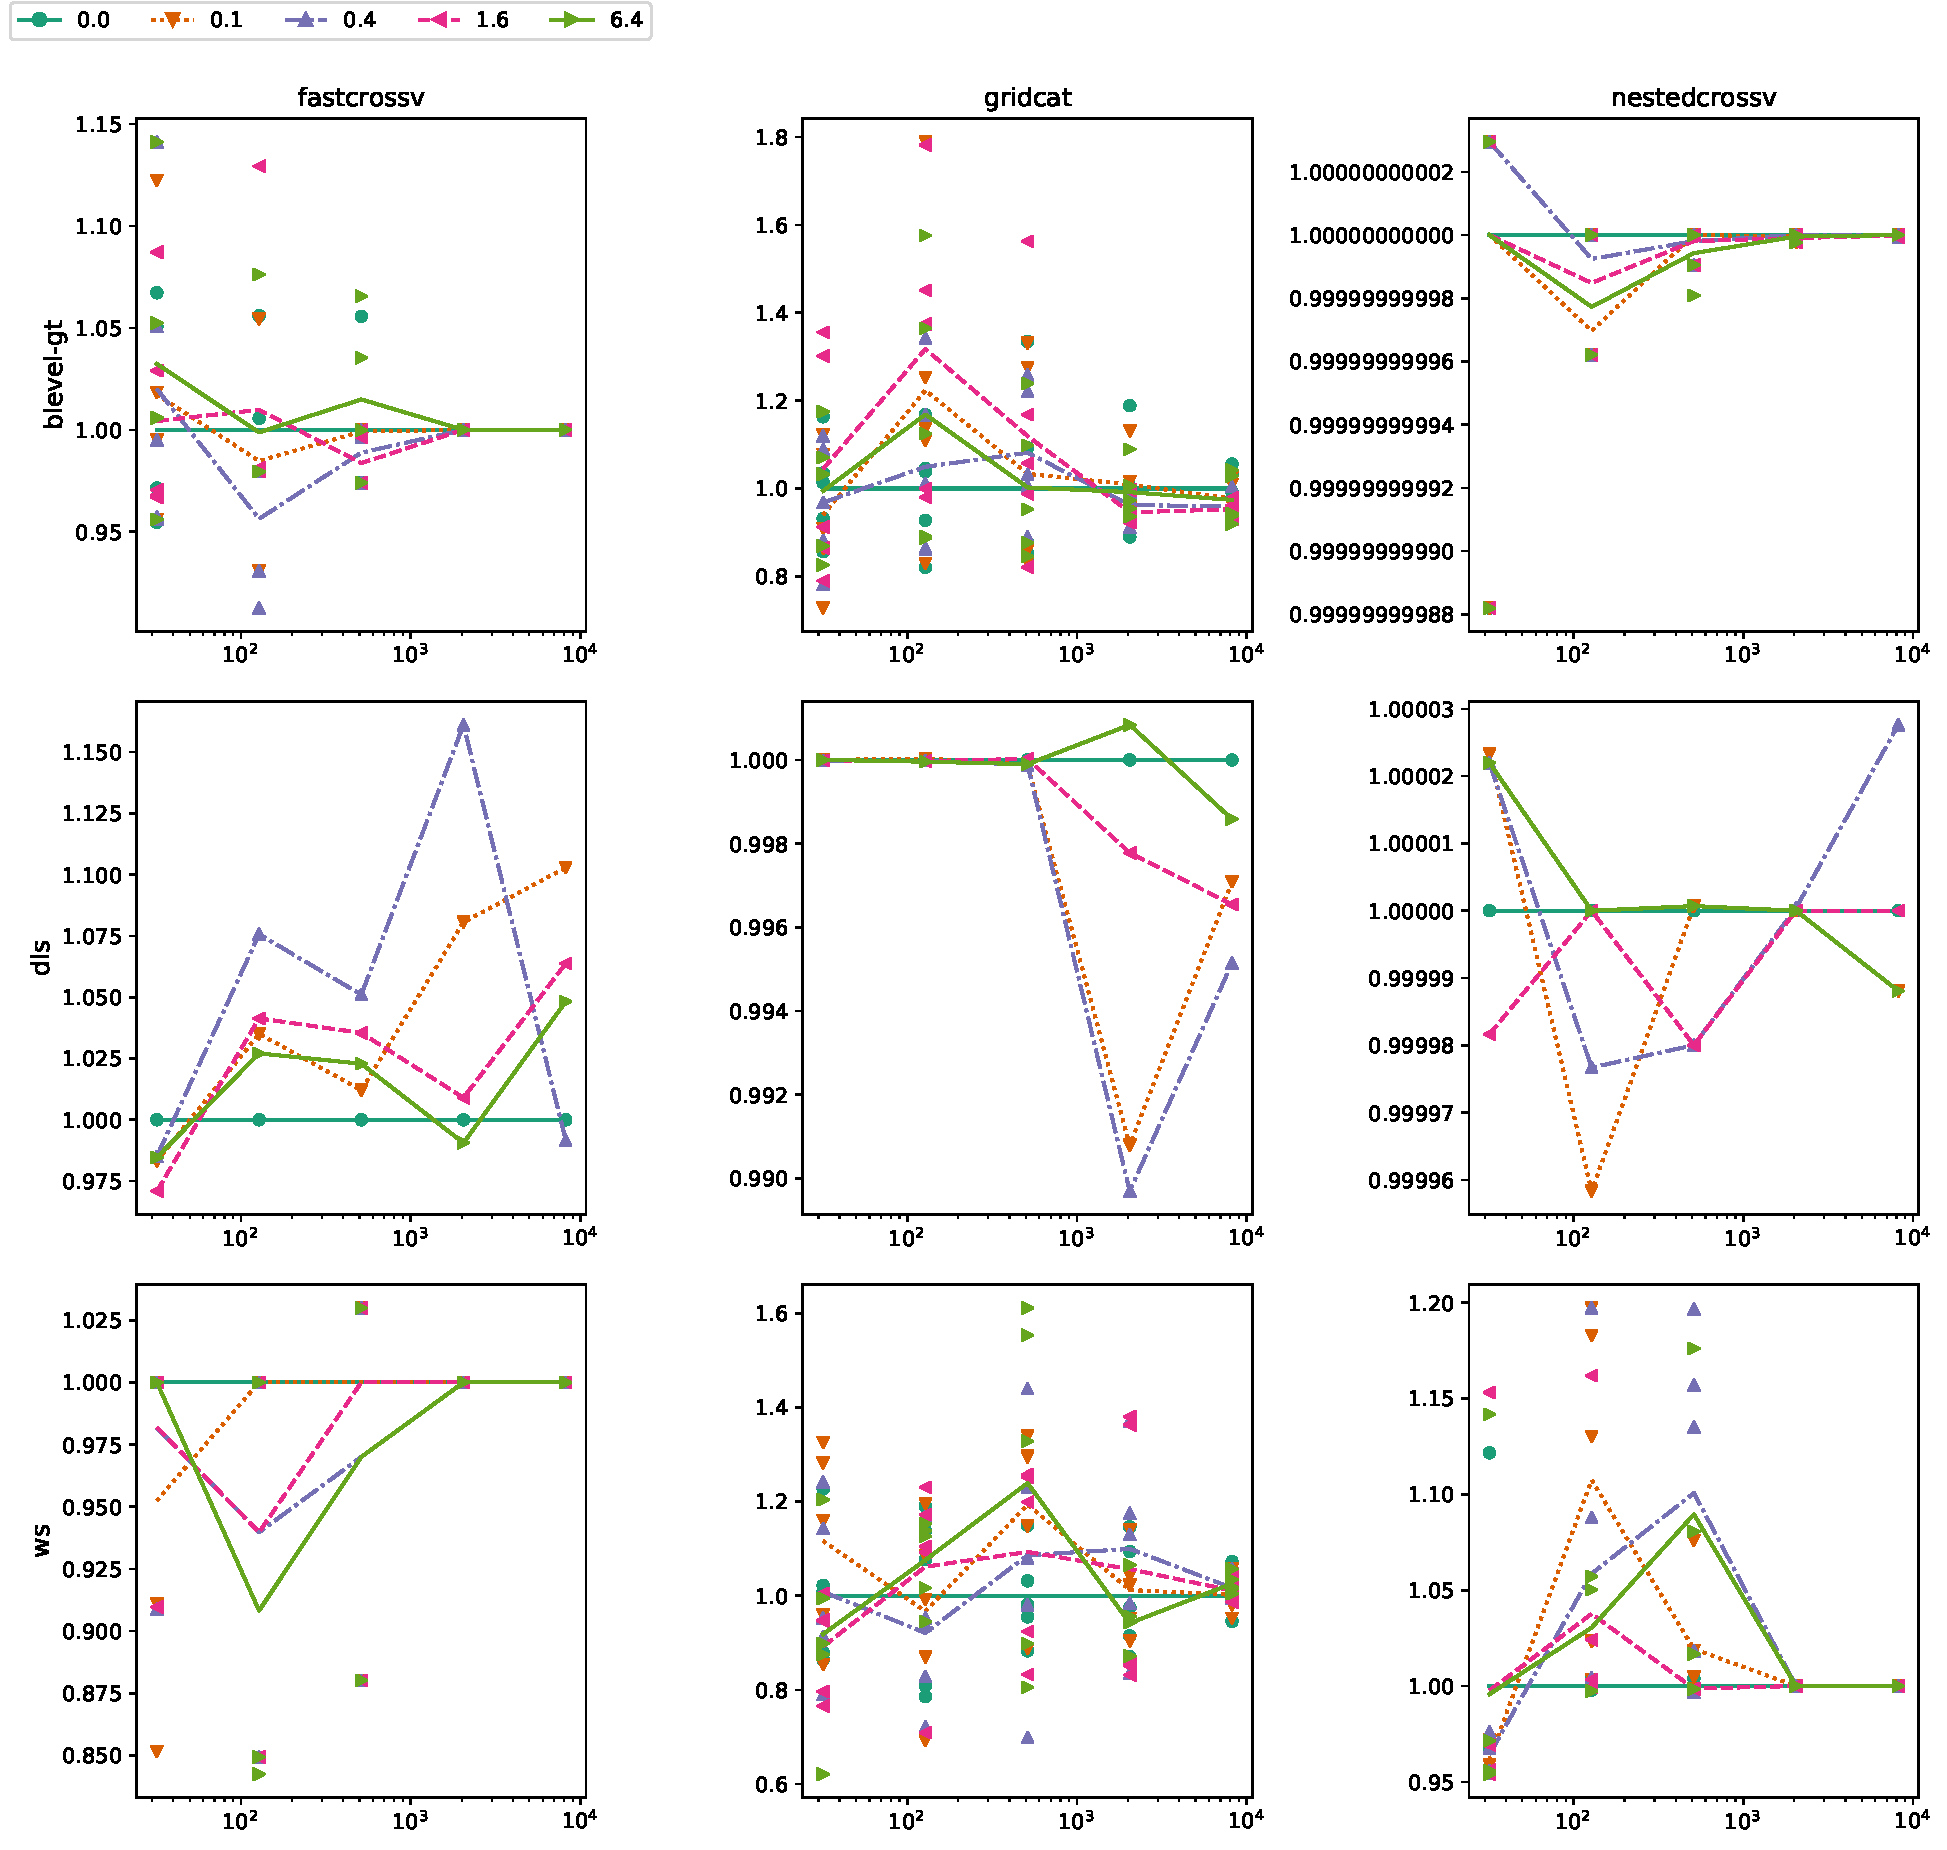
\includegraphics[width=0.8\textwidth]{imgs/estee/charts/irw-32x4-schedtime-score}\\
	{\small horizontal axis: bandwidth [MiB/s]; vertical axis: makespan normalized to
	$\gls{msd}=0$}
	\caption{Comparison of \acrshort{msd}; cluster 32x4}
	\label{fig:estee-chart-irw-msd}
\end{figure}

In~\Autoref{fig:estee-chart-irw-msd}, we can observe the effect of \gls{msd} on graphs from the
\emph{irw} dataset, with the $32x4$ cluster configuration. The Y axis
is normalized with respect to the configuration where \gls{msd} is zero. The results
show that the effect of \gls{msd} is relatively limited. There does not seem to be
any clear correlation or pattern that would suggest that a smaller \gls{msd}
consistently improves performance of a scheduler. Although interestingly, a higher
\gls{msd} value caused several makespan improvements, especially on the
\emph{gridcat} task graph.

This is another example of the non-trivial effect of scheduler heuristics. Increasing the
\gls{msd} leads to a batching effect, where the scheduler is allowed to make
decisions less often, but it has knowledge of more task events (that have arrived during the delay)
during each decision. Whether this helps its performance, or hurts it, depends on the specific
scheduler implementation and the task graph that it executes.

\subsubsection*{Information modes}

\begin{figure}
	\centering
	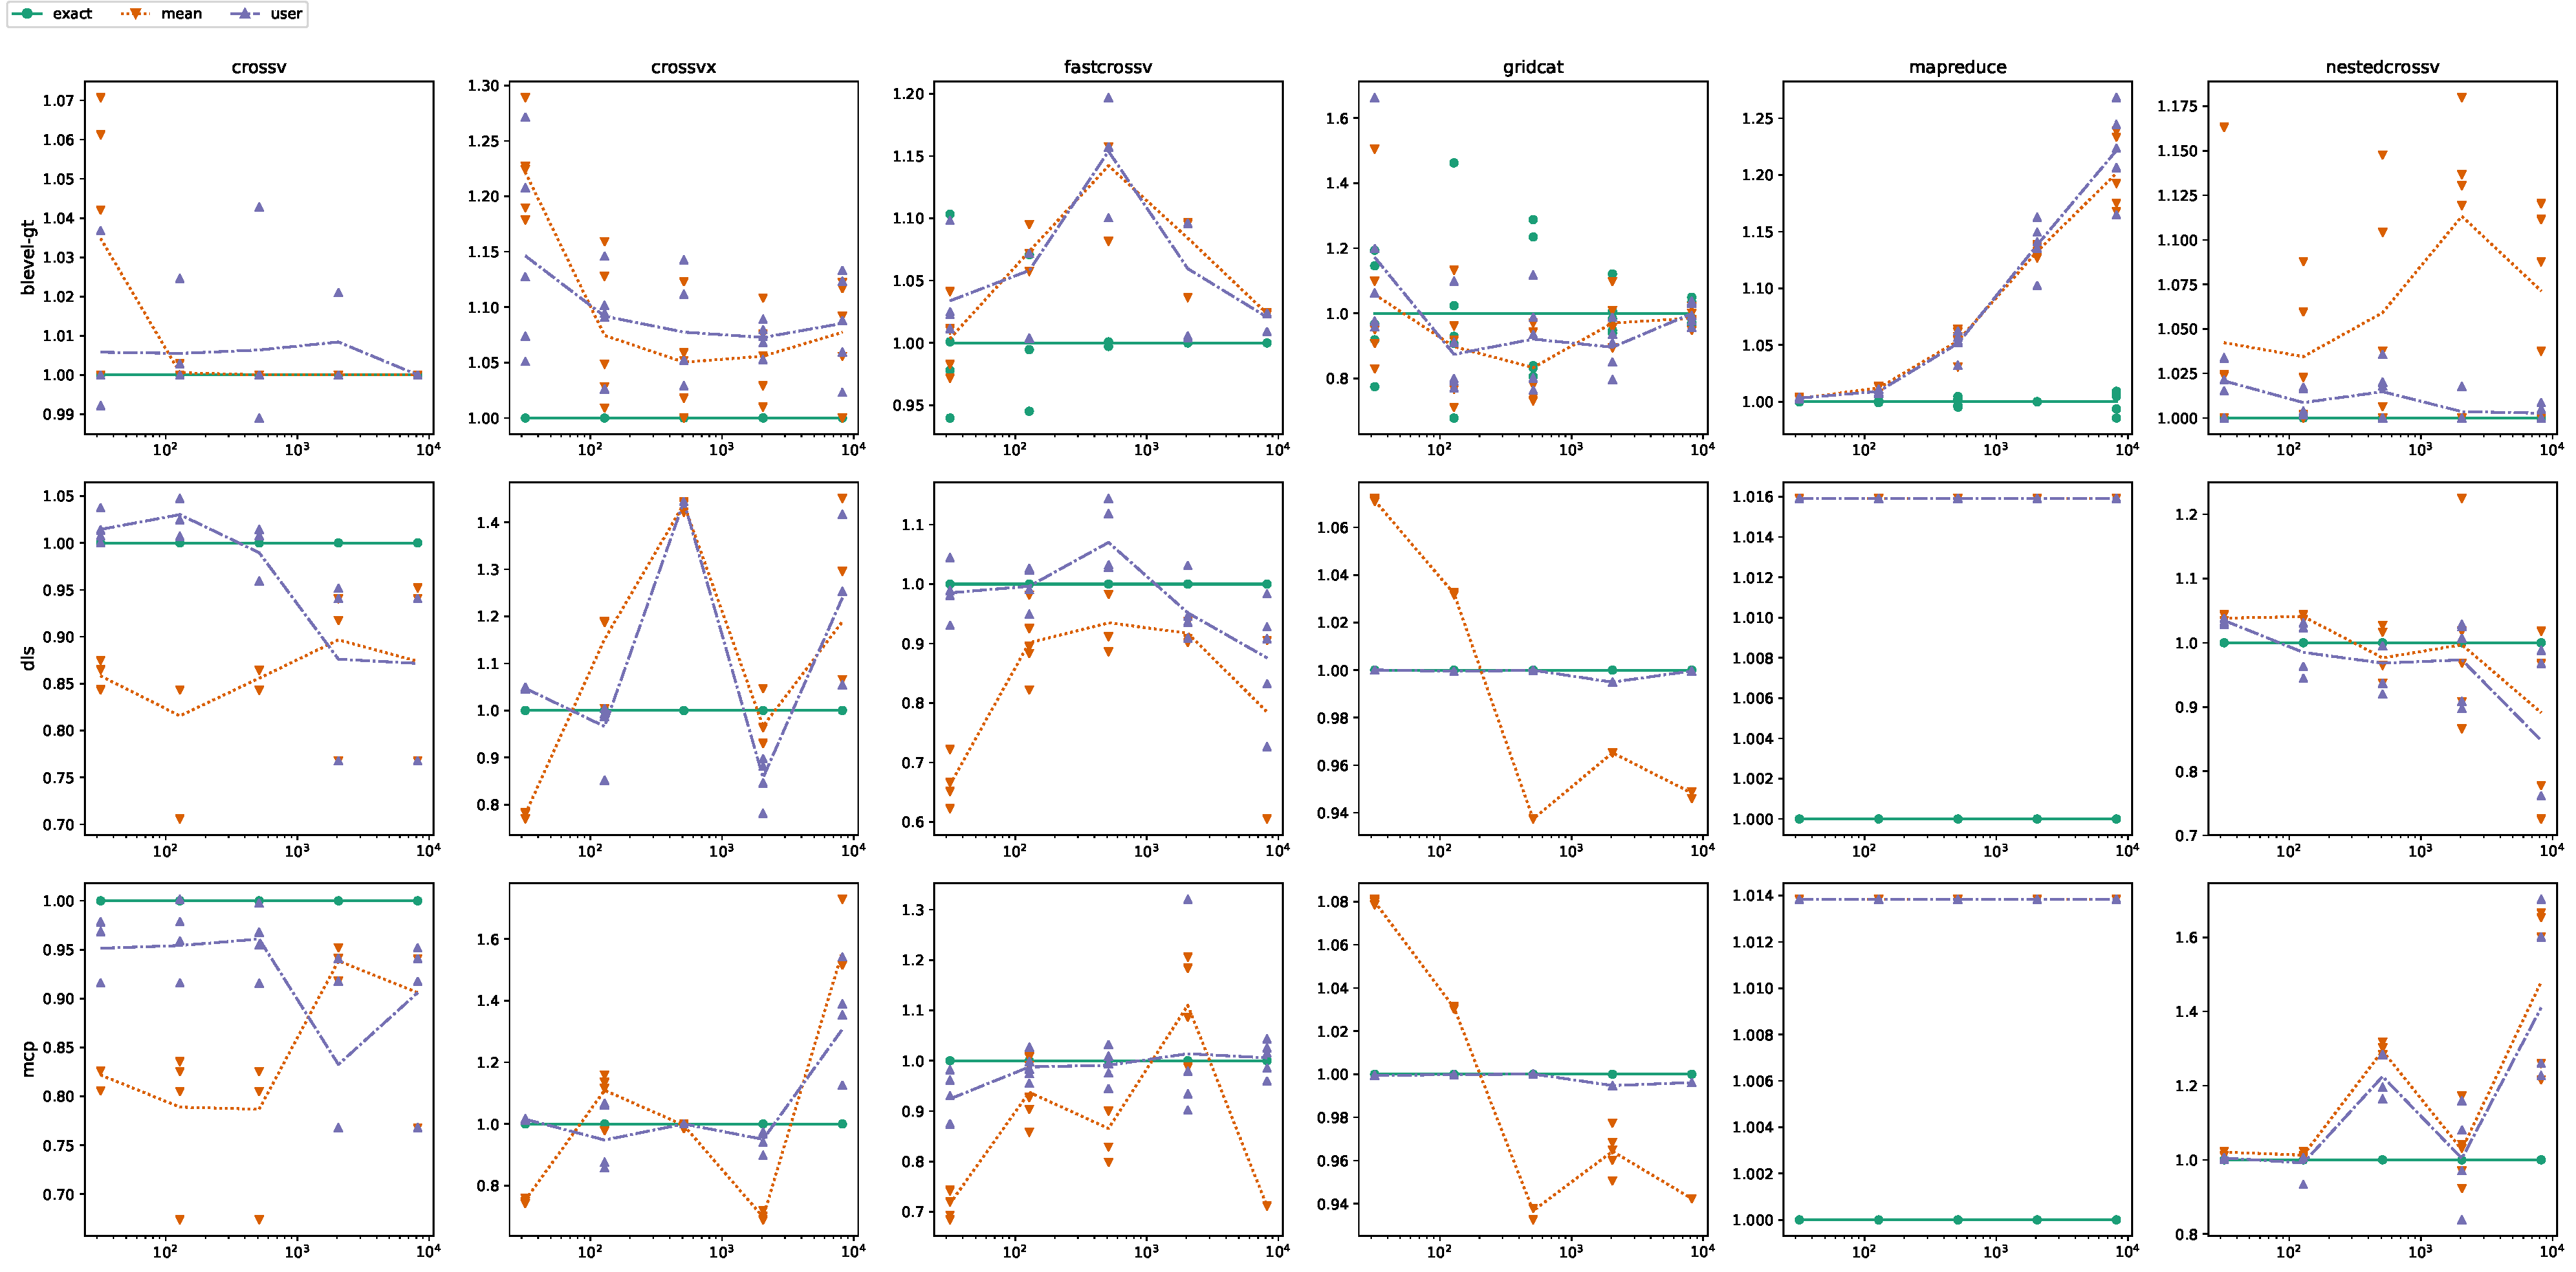
\includegraphics[width=\textwidth]{imgs/estee/charts/irw-32x4-imode-score}\\
	{\small horizontal axis: bandwidth [MiB/s]; vertical axis: makespan normalized to
	\emph{exact}
	imode; row: scheduler; cluster $32x4$} \caption{Comparison of information modes (\emph{irw} dataset)}
	\label{fig:estee-chart-irw-imode}
\end{figure}

%\begin{figure}
%	\centering
%	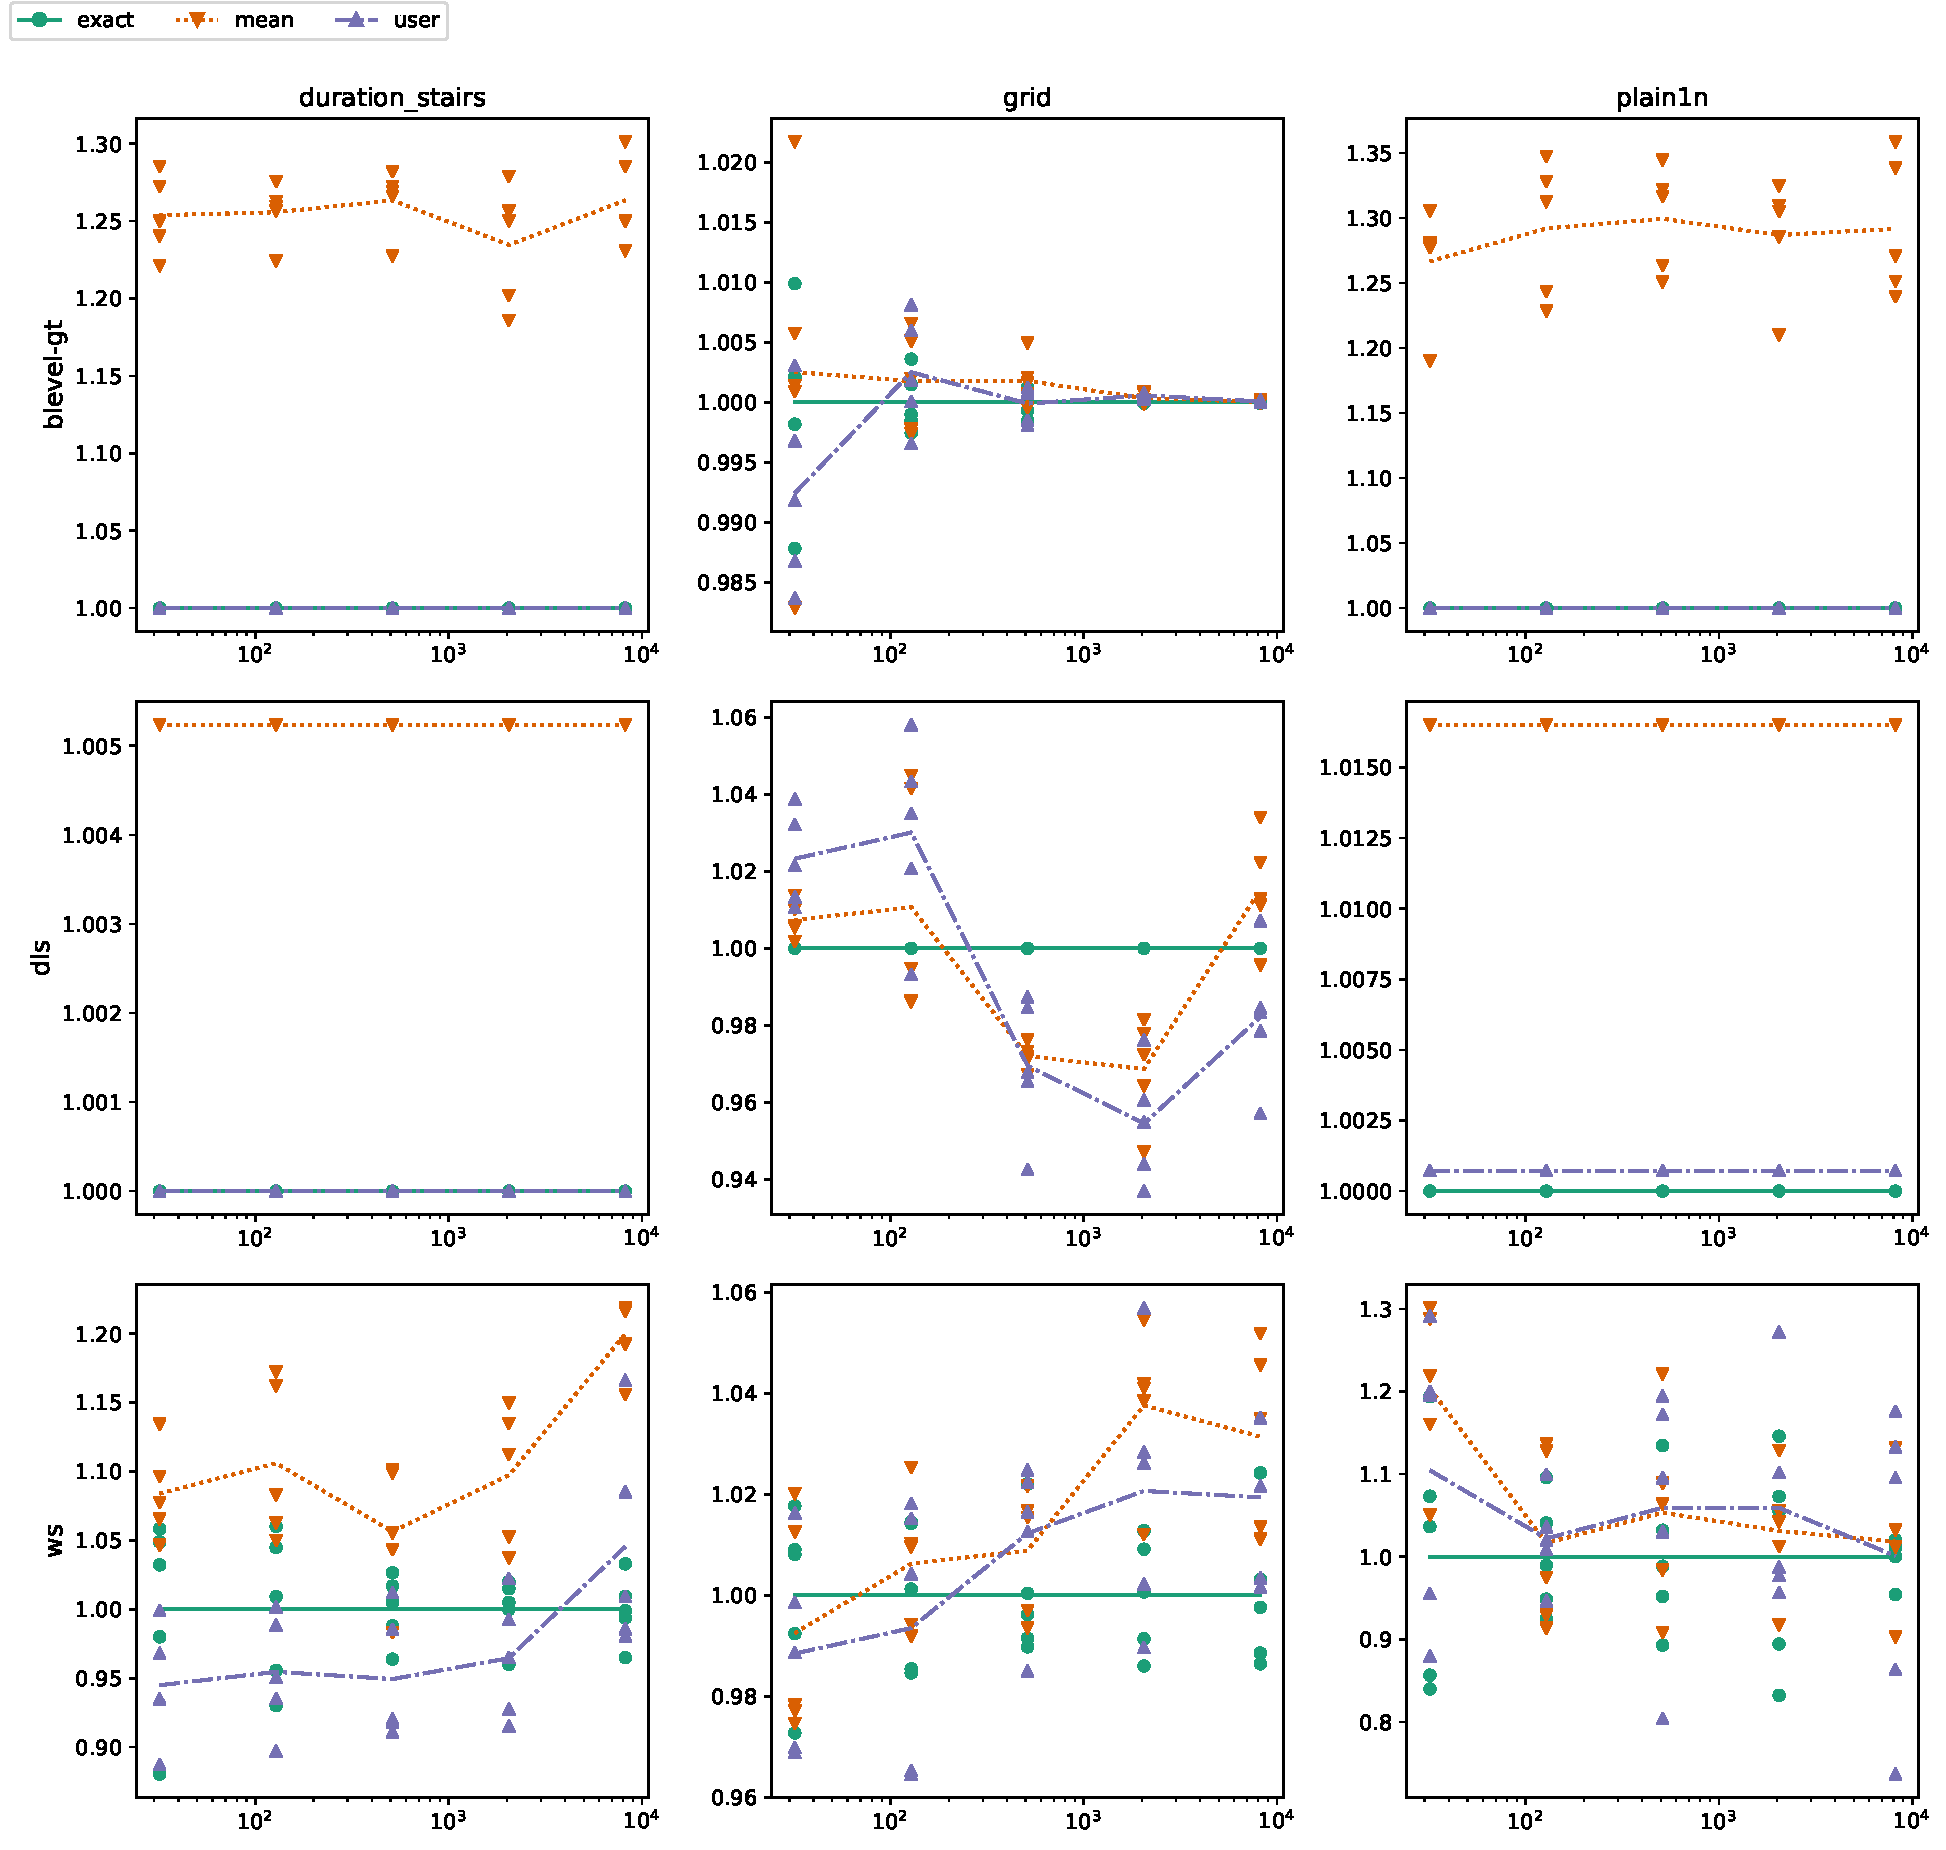
\includegraphics[width=0.8\textwidth]{imgs/estee/charts/elementary-32x4-imode-score}\\
%	{\small horizontal axis: bandwidth [MiB/s]; vertical axis: makespan normalized to
%	\emph{exact} average; row: scheduler; cluster $32x4$}
%   \caption{Comparison of information modes (\emph{elementary} dataset)}
%   \label{fig:estee-chart-elementary-imode}
%\end{figure}

\Autoref{fig:estee-chart-irw-imode} compares makespans of several scheduler and task graph combinations
from the \emph{irw} dataset on a $32x4$ cluster, with different
information modes being used. The results are normalized to the mean makespan of the default
\emph{exact} information mode. In general, the effect of information modes is more
significant than the effect of the \acrlong{msd}.

An intuitive expectation would be that with more precise task duration information, the scheduler
will be able to produce a shorter makespan, and this is indeed what happens in several cases, e.g.\
on the \emph{mapreduce} and \emph{nestedcrossv} task graphs with the
\emph{blevel-gt} scheduler, where the makespan is up to 25\% longer when task durations are
not exactly known.

However, there are also opposite cases, for example the \emph{dls} and
\emph{mcp} schedulers produce better results on several task graphs when they take
only the \emph{mean} task duration into account. This further shows the effect of
scheduler heuristics, which can produce worse results even when presented with more accurate data
input (and vice versa).

One factor that makes it more difficult for the scheduler to accurately estimate the network
transfer durations and thus make optimal use of the knowledge of task durations is that with the
max-min network model, the scheduler knows only a lower bound on the communication costs, even if
it knows the exact data size in advance. While it has access to the maximum bandwidth of the
network, it does not know the current (and most importantly, future) network utilization; thus it
has only a crude estimation of the real transfer duration.

\subsection{Validation}
It is challenging to validate the performance of different task schedulers in actual
(non-simulated) task runtimes. Schedulers tend to be deeply integrated into their task runtime in
order to be as performant as possible. That makes it difficult, or even infeasible, to replace the
scheduling algorithm without also modifying large parts of the task runtime. Furthermore, some
scheduling approaches might not even be compatible with the architecture of the runtime as a whole.
For example, work-stealing schedulers perform a lot of communication between the server and the
workers (potentially even between the workers themselves), and if the runtime does not implement
the necessary infrastructure for facilitating these communication patterns, then implementing a
work-stealing scheduler into such a runtime might amount to rewriting it from scratch.

In order to at least partially validate our simulation results, we have decided to use a modified
version of the \dask{}~\cite{dask} task runtime as a validation
framework. Apart from validating results from the \estee{} simulations, we have also
used this modified version of \dask{} to perform other experiments and benchmarks
that are described in~\Autoref{ch:rsds}, which also depicts the architecture of
\dask{} and our performed modifications in detail.

\dask{} is written in Python, which makes it relatively easy to modify and patch.
It uses a work-stealing scheduler by default, and even though it is relatively deeply integrated
within the \dask{} runtime, we were able to implement three simple alternative
scheduling algorithms into it\footnote{The modified version of \dask{} with these implemented schedulers can be found at
\url{https://github.com/Kobzol/distributed/tree/simple-frame-sched}.}, which correspond as closely as possible to
the \emph{random}, \emph{blevel} and \emph{tlevel} schedulers from
\estee{}. The default work-stealing scheduler was compared with our work-stealing
implementation of the \emph{ws} scheduler.

Apart from implementing new schedulers into \dask{}, there were several issues that
we had to solve to make sure that the comparison between the simulated and the real environment is
as fair and accurate as possible.

The absolute makespans of task graphs simulated by \estee{} and task graphs executed
by \dask{} cannot be compared directly, because there are many aspects of the
operating system, network, implementation of \dask{} itself and system noise that
\estee{} can not fully simulate. Therefore, since the primary goal of our task
scheduler experiments was to compare the relative performance of individual schedulers, we have
decided to compare the relative makespans normalized to a reference scheduler
(\emph{blevel}), to test if the makespan ratios between the schedulers is similar in
simulation and in real execution.

In the scheduler benchmarks, we have used many task graphs generated by the \estee{}
task graph generator. However, it would not be possible to perfectly replicate task durations of
these generated graphs in \dask{}. Therefore, we have approached this problem from
the other direction. We have executed several task graphs in \dask{}, and recorded
their execution traces, so that we would have a completely accurate representation of all the
executed task durations and data object sizes, which we could then accurately replicate in the
simulated \estee{} environment. The recorded task graphs will be described
in~\Autoref{sec:rsds-dask-overhead-analysis} and they can also be found in~\cite{rsds}. We have
executed these workflows with a $24x2$ cluster ($24$ cores on two nodes), which corresponds
to two nodes of the Salomon~\cite{salomon} cluster, on which were the \dask{} workflows executed.
Each actual execution and simulation was performed three times.

\begin{figure}
	\centering
	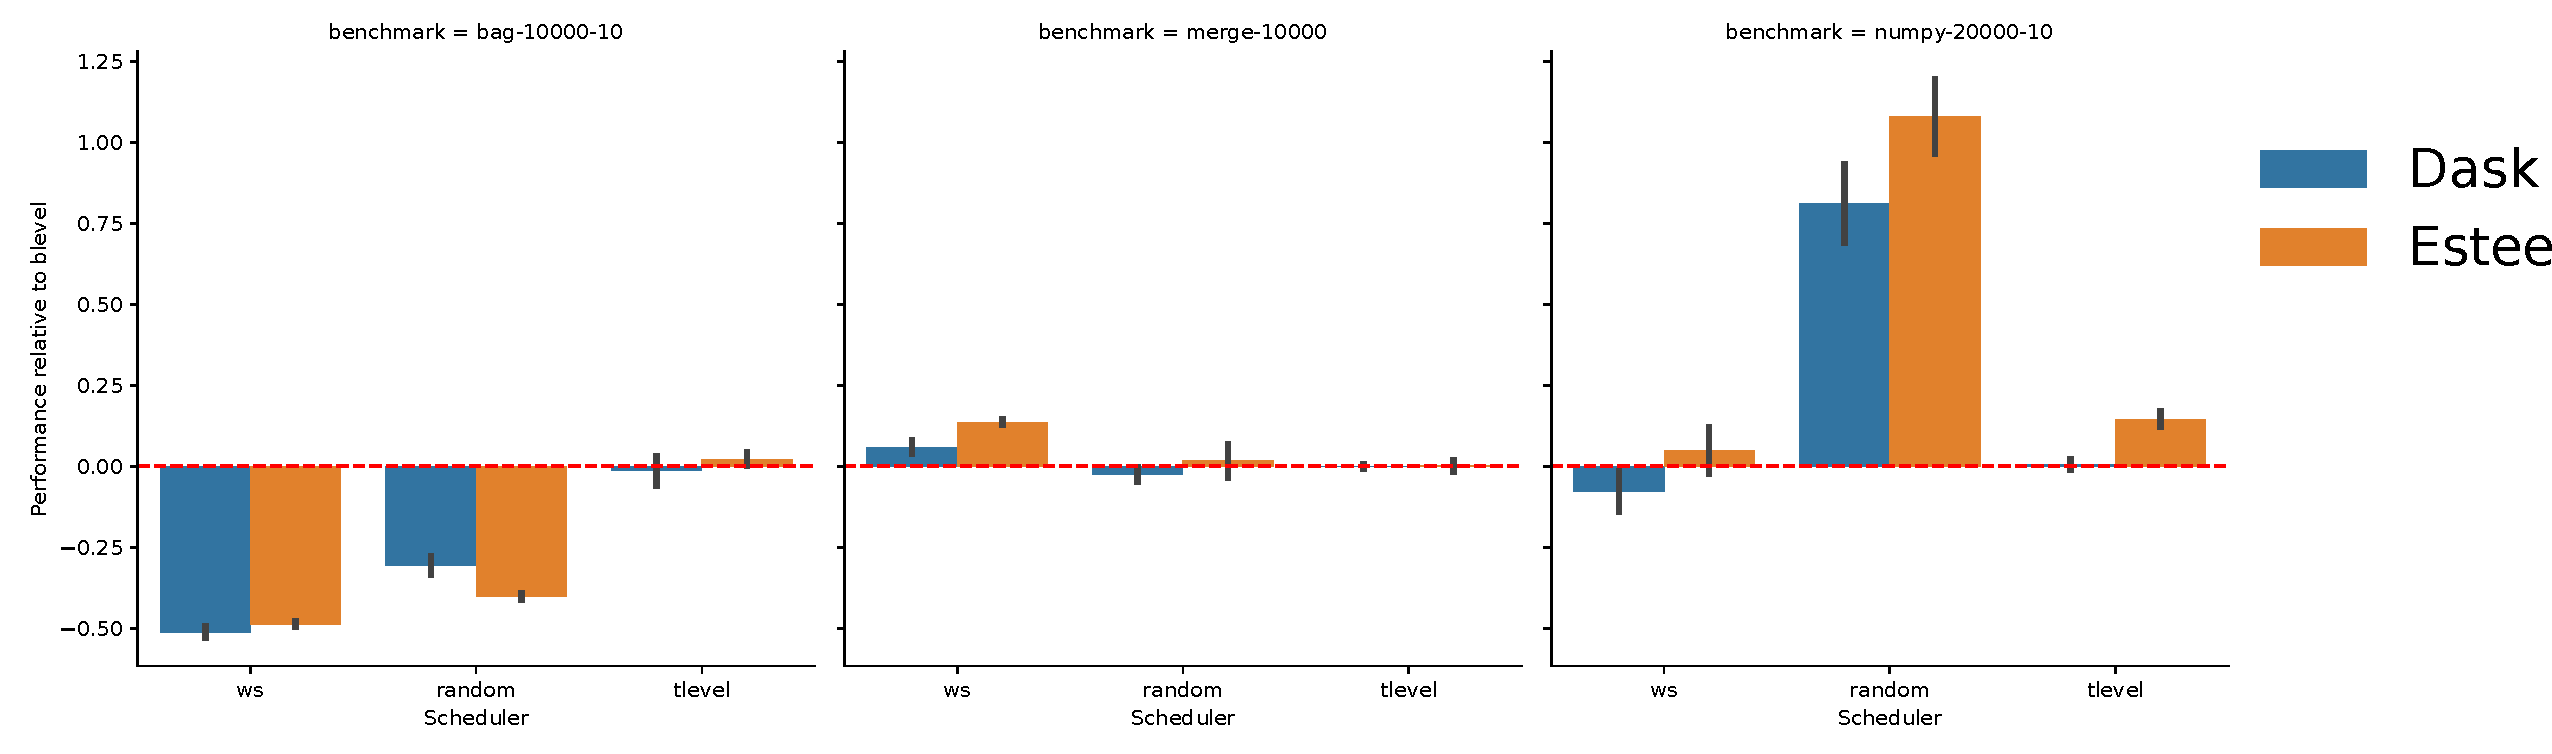
\includegraphics[width=\textwidth]{imgs/estee/charts/estee-validation}\\
	\caption{Scheduler performance relative to \emph{blevel} in \dask{} and \estee}
	\label{fig:estee-validation}
\end{figure}

\Autoref{fig:estee-validation} shows the results of the validation comparison for three selected
task graphs\footnote{Extended validation results can be found in~\cite{estee}.}. The performance of each scheduler was normalized to the
makespan of the \emph{blevel} scheduler within the same environment (either
\estee{} or \dask{}). Note that the relative ratios were centered
around zero by subtracting $1$ from them, to focus on the relative differences.
For example, if a task graph execution had a makespan of \SI{100}{\second} with the \emph{blevel} scheduler, but \SI{110}{\second} with the \emph{ws} scheduler, the ratio of the \emph{ws} scheduler would be
$0.1$. If the simulation was perfect, the two columns for each scheduler would
have the same height.

The first chart shows a situation where changing the scheduler resulted in large changes in
makespans, and \estee{} was able to simulate these changes relatively accurately, and reflect
the results measured in \dask{}. The second chart demonstrates a situation where
all schedulers produce similar makespans; therefore, in this case the scheduling algorithm does not
seem to be that important. \estee{} was again able to estimate that the differences
between schedulers will be small. In the third chart, we see that \estee{} was
systematically overestimating the makespans of all three schedulers (with respect to the reference
scheduler). The most important difference was in the \emph{ws} scheduler, where the
simulated result claims that it is slower than \emph{blevel}, while in reality it was
slightly faster. The work-stealing implementation in \dask{} is complex, and in
this case it was able to outperform \emph{blevel} in a way that \estee{}
was not able to simulate.

To summarize the average error of the simulated results, we took the relative makespans of the
individual schedulers w.r.t.\ the reference \emph{bevel} scheduler, and calculated the
difference between the executed and simulated relative makespan. The geometric mean of these
differences across all measured benchmarks was $0.0347$, which suggests that the
differences between the execution and simulation were relatively small; the simulated makespans
were usually within just a few percent off the actual makespan duration.

\section*{Summary}
We have implemented a set of well known scheduling heuristics, prepared a benchmark dataset
containing task graphs of different types and scales and designed a simulation environment for task
scheduler experimentation. We have conducted a series of reproducible benchmarks using that
environment, in which we have analyzed the effect of network models, minimal scheduling delays,
information modes and worker selection strategy on the behavior of the implemented schedulers, and
also compared their relative performance.

Our attempts to implement existing scheduling algorithms in \estee{} and reproduce
the results of previous scheduler benchmarks have shown that various implementation details which
are often missing from the algorithm's description (like the precise worker selection strategy) can
have a large effect on the final performance of the scheduler. Furthermore, we have been able to
confirm our hypothesis that the naive network model used in several existing works can result in
very inaccurate simulation results.

Combined with the fact that the source code of many published scheduling algorithms or surveys is
not open-source, it is difficult (even nigh impossible) to accurately reproduce their performance
results. We have tried our best to make all available source-code, benchmark datasets and the
results of our experiments public, to make them easy to reproduce and thus avoid this issue.

%Our analysis has shown that despite its simplicity, the foundational \gls{hlfet}
%algorithm~\cite{hlfet1974} (\emph{b-level}) produces high quality schedules in various scenarios and should
%thus serve as a good baseline scheduler for task runtimes. It can be complemented with
%work-stealing, which is able to dynamically react to load imbalances of individual workers.

We have demonstrated that even a completely random scheduler can be competitive with other
scheduling approaches for certain task graphs and cluster configurations.
This supports the conclusion made in~\cite{wang2018list}, where the authors have also observed
that relatively simple scheduling algorithms can be competitive, and more complex algorithms are
useful mostly for special situations and edge cases, where the simple heuristics might fail to
produce reasonable results.

The \acrlong{msd} had a smaller effect in our simulations than we have expected. This
hints that it might be possible to reduce the scheduling overhead (by invoking the scheduler less
often) without sacrificing schedule quality, but this will be highly dependent on the specific task
runtime implementation.

The effect of different information modes turned out to be significant, although it is unclear
whether schedulers can leverage the additional information about exact task durations when facing
unpredictable network conditions.

The implemented \estee{} simulator enables simple prototyping of task schedulers and
also allows simulating execution of various task graphs. We hope that it could have further
potential to simplify the development and evaluation of novel task schedulers.

Through our experiments presented in this chapter, we have learned more about the effect
of scheduling algorithms on the performance of task graphs. We have identified a
performant baseline scheduling approach, work-stealing combined with the \emph{b-level} heuristic,
which we have further leveraged in work described in the following two chapters.

Although task scheduling is an important factor, it is not the only aspect that contributes to the
overall overhead and performance of task runtimes. The following chapter will examine
the runtime overhead and scalability of a state-of-the-art task runtime in more detail.


	\chapter{Task runtime optimization}
	\label{ch:rsds}
	This chapter delves further into the performance aspects of task graph execution
on \gls{hpc} clusters. After performing the task scheduling experiments using \estee{}, our next goal
was to find out how do other parts of task runtimes (other than the scheduler) affect task graph makespans,
and also to validate some of the rather surprising results of our
experiments, for example the competitiveness of the random scheduler, in a non-simulated setting.
In order to do that, we had to move from a simulator to a task runtime that can execute task graphs on an
actual distributed cluster.

As was already discussed in~\Autoref{ch:sota}, there is a large amount of existing task runtimes
that are being used on \gls{hpc} systems, which could be used as a test vehicle for our experiments.
After evaluating several of them, we have decided to examine the \dask{}~\cite{dask} task runtime, for
the following reasons.
\begin{itemize}
	\setlength\itemsep{0.1em}
	\item It is very popular within the scientific community~\cite{dask-user-survey}, therefore any
	      insights on how it could be improved could benefit a wide range of users.
	\item It is implemented in Python, which makes it relatively easy to modify.
	\item It is quite versatile, because it allows executing arbitrary task graphs with dependencies and data
	      objects, and completely supports the task programming model described in~\Autoref{ch:taskgraphs}.
	\item It uses a fairly standard distributed architecture with a centralized server that creates task
	      schedules and assigns tasks to a set of distributed workers. This maps well to the cluster
	      architecture used by \estee{}, and also to \gls{hpc} clusters in
	      general.
\end{itemize}

In terms of task scheduling, \dask{} uses a work-stealing scheduler, which has
been tuned extensively over several years to support various use-cases and to provide better
scheduling performance. Yet it is unclear whether additional effort should be directed into
improving the scheduler, or if there are another bottlenecks which should be prioritized.

To answer that question, we have analyzed the runtime performance and the bottlenecks of
\dask{} in
\emph{Runtime vs Scheduler: Analyzing Dask's Overheads}\footnote{Note that this line of research follows after the task scheduler analysis described previously
in~\Autoref{ch:estee}, even though it was published at an earlier date.}~\cite{rsds}. This work
provides the following contributions:
\begin{enumerate}
	\item We have created a set of benchmarks containing diverse task graphs implemented in
	      \dask{}. This benchmark set was then used to analyze \dask{}'s
	      performance in various \gls{hpc}-inspired scenarios. We have evaluated the
	      per-task-overhead and scalability of \dask{} and compared how different task
	      scheduling algorithms affect its performance.
	\item We demonstrate that even a naïve (completely random) scheduling algorithm can be
		  competitive in many common situations with the sophisticated hand-tuned work-stealing scheduler used in
	      \dask{}.
	\item We provide \rsds{}, an alternative \dask{} server that is
	      backwards-compatible with existing \dask{} programs and provides significant
	      speed-up vs the baseline \dask{} server in many scenarios, despite using a
	      simpler task scheduler implementation.
\end{enumerate}

Various descriptions of task graph benchmarks, \dask{} and
\rsds{} used in this chapter were adapted from this
publication~\cite{rsds}.

\workshare{I have collaborated on this work with Ada Böhm, we have both contributed to it equally. Source code contribution statistics for
\rsds{} can be found on GitHub\footnoteurl{https://github.com/it4innovations/rsds/graphs/contributors}.}

\section{\dask{} task runtime}
\label{sec:rsds-dask}
% TODO: place Dask into SOTA and describe it more, if not already done in the SOTA chapter
\dask{} is a distributed task runtime implemented in Python that can
parallelize and distribute Python programs. It offers various programming interfaces
(\glspl{api}) that mimic the interfaces of popular Python packages. For example,
\emph{Dask DataFrame} copies the \texttt{pandas}\footnoteurl{https://pandas.pydata.org}
interface for table processing and database operations, \emph{Dask Arrays} copies the
\texttt{numpy}\footnoteurl{https://numpy.org} interface for tensor computations and
\emph{Dask ML} copies the \texttt{scikit-learn}\footnoteurl{https://scikit-learn.org}
interface for machine learning. Thanks to this interface compatibility, existing Python programs
leveraging these libraries can often be parallelized with \dask{} by changing
only a handful of lines of code.

This is demonstrated in~\Autoref{lst:dask-array-example} and~\ref{lst:dask-dataframe-example-2}, which show two
small Python programs that leverage the \emph{Dask Arrays} and \emph{Dask DataFrame}
\gls{api} respectively. Notably, the only difference between these programs
(which are leveraging \dask{}, and thus can be parallelized), and a standard
sequential version, is the change of imports from \texttt{numpy} and
\texttt{pandas} to \dask{} Python modules.

\begin{listing}[h]
	\caption{Example of a Python program that leverages the \dask{} Array
	\gls{api}}
	\label{lst:dask-array-example}
	\begin{minted}[fontsize=\small]{python}
# import numpy as np
import dask.array as np

x = np.random.random((10000, 10000))
y = (y * 2 + x.T).mean(axis=1)
	\end{minted}
\end{listing}

\begin{listing}[h]
	\caption{Example of a Python program that leverages the \dask{} DataFrame
	\gls{api}}
	\label{lst:dask-dataframe-example-2}
	\begin{minted}[fontsize=\small]{python}
# import pandas as pd
import dask.dataframe as pd

df = pd.read_csv("data.csv")

df2 = df[df.y > 0]
df3 = df2.groupby("name").x.std()
	\end{minted}
\end{listing}

\subsection*{Computational model}
\dask{} automatically transforms Python code leveraging these
\glspl{api} into a task graph, which is then executed in parallel, possibly on
multiple nodes of a distributed cluster. This enables almost transparent parallelization of
sequentially looking Python code. However, apart from these high-level interfaces, it is also
possible to build a task graph manually, using the \emph{Futures} interface, to define
complex computational workflows.

The core computational abstraction of \dask{} is a \emph{task graph},
which corresponds closely to the definition of task graphs in \Autoref{ch:taskgraphs}. Each
task represents a single invocation of a Python function. The return value of the function forms
its \emph{output} (a data object), and the arguments of the function invocation define the
\emph{inputs} of the task.

One important aspect of the mapping between Python code and task graphs in
\dask{} is the concept of \emph{partitions}. It is a configuration
parameter that essentially controls the granularity of tasks created by \dask{}
out of Python code that uses its \glspl{api}. For example, a single line of Python
code that performs a query over a \texttt{pandas}-like table (also called DataFrame)
will be eventually converted to a set of individual tasks that e.g.\ perform the query on a subset
of the table's rows. The selected number of these tasks (or partitions) is crucial, since it
determines how effectively will the operation be parallelized. Too few (large) tasks can cause
computational resources to be under-utilized, while too many (small) tasks can overwhelm the
\dask{} runtime.

\subsection*{Architecture}
\dask{} supports multiple computational backends that can execute the task
graphs generated from Python code. The default backend is able to execute the task graph in a
parallelized fashion on a local computer, but there is also a distributed backend called
\emph{Dask/distributed}\footnoteurl{https://distributed.dask.org}
(or simply \emph{distributed}), which is able to execute task graphs on
multiple nodes. Since this backend is most relevant for task graph execution on distributed and
\gls{hpc} clusters, our experiments focus solely on this backend, and any further
reference to \dask{} in this text will assume that it uses the
\emph{distributed} backend.

In terms of architecture, \emph{distributed} is composed of three main components: the
\emph{client}, the \emph{server} and the \emph{worker}. A
single server and an arbitrary number of workers deployed together (e.g.\ on a local machine or a
distributed system) form a \dask{} cluster.

The \emph{client} is a user-facing library that offers various
\glspl{api} used to define computations in Python that can be converted into a task
graph. Once the user defines the computation, the client can connect to the
\dask{} cluster (more specifically, to the server), submit the task graph, wait
for it to be computed and then gather the results. The client can build the whole task graph
eagerly on the user's machine and then send it to the server for processing, however this can
consume a lot of memory and network bandwidth if the task graph is large. For certain types of task
graphs, clients are able to send a much smaller, compressed abstract representation of the task
graph, which is only expanded on the server lazily, which can help reduce memory and network
transfer bottlenecks.

The \emph{server} is the central component of the cluster, which communicates with
the workers and clients through a network, usually a \gls{tcpip} connection,
handles client requests, coordinates task execution on workers and manages the whole
\dask{} cluster. Its main duty is to process task graphs submitted by clients,
by assigning individual tasks to workers, in order to parallelize the execution of the submitted
task graph and in turn efficiently utilize the whole cluster. It uses a sophisticated work-stealing
scheduler that uses many heuristics, which have been tuned for many years. Some of them are
described in the \dask{} manual\footnoteurl{https://distributed.dask.org/en/latest/work-stealing.html}.

The scheduler works in the following way: when a task becomes \emph{ready}, i.e.\
all its dependencies are completed, it is immediately assigned to a worker according to a heuristic
that tries to minimize an estimated start time of the task. This estimate is based primarily on any
potential data transfers that would be incurred by moving the data objects of tasks between
workers, and also the current occupancy of workers. When an imbalance occurs, the scheduler tries
to steal tasks from overloaded workers and distribute them to underloaded workers. The scheduler
also assigns priorities to tasks, which are used by workers to decide which tasks should be
computed first.

The \emph{worker} is a process which executes tasks (consisting of serialized Python
functions and their arguments) that are assigned and sent to it by the server. Workers also
communicate directly amongst themselves to exchange task outputs (data objects) that they require
to execute a task. Tasks assigned to a worker are stored in a local queue, tasks are selected from
it based on their priorities. Each worker can be configured to use multiple threads, some of which
handle network (de)serialization and \gls{io} in general, while the rest is
assigned for executing the tasks themselves. However, there is an important caveat that can limit
the parallel execution of tasks within a worker, which is described below.

\subsection*{Bottlenecks}
The primary bottlenecks that limit the efficiency of \dask{} are related to the
programming language used for its implementation. All described components (server, worker and
client), are implemented in Python, which has non-trivial consequences for its performance, because
the Python language is not well suited for implementing high-performance infrastructure. The most
commonly used Python interpreter (CPython\footnoteurl{https://github.com/python/cpython}) does not allow programmers to
make optimal use of hardware in general in an easy way, due to its indirect memory layout and
automatic memory management that pervasively uses reference-counting.

Crucially, there is a specific quirk of this interpreter that can severely reduce the performance
of task graph execution in \dask{}, and specifically affects the
characteristics of its workers. The CPython interpreter infamously uses a shared, per-process lock
called \gls{gil}, which synchronizes access to the interpreter internals. This
means that when a Python program is interpreted using CPython, only a single thread that executes
Python code can make progress at the same time. It is still possible to achieve concurrency with
multiple Python threads (e.g.\ by using blocking \gls{io}, which releases the
\gls{gil} while the thread is blocked), but not parallelism, under this design.
There are some caveats to this, notably code written using native Python extensions (most commonly
written in \texttt{C}, \texttt{C++} or \texttt{Rust})
can run truly in parallel with other Python threads, but only if it opts into releasing the global
lock, and if it does not need to interact with the Python interpreter at all while the native code
is running.

The \gls{gil} issue does not impact only \dask{}, of course.
It is a pervasive issue across the whole Python ecosystem. There have been multiple attempts over
the years to remove the \gls{gil} from CPython, but they have not been successful
yet. The most recent attempt has progressed the furthest, and it has been accepted as a
\gls{pep} 703~\cite{pep703}, so it is possible that the
\gls{gil} will be eventually removed from CPython. However, even if this proposal
is eventually adopted, it will probably take years before Python packages and programs will fully
adapt to the change.

The presence of the \gls{gil} poses a challenge for \dask{}
workers. Unless a task executed by a worker releases the \gls{gil} (which essentially means that the task either has to be
implemented in native code, or it needs to block on an \gls{io} operation), it will block
all other tasks from executing at the same time. Therefore, a single \dask{}
worker can only execute at most one non-native and non-blocking task at once, which can potentially
severely limit its throughput and the efficiency of task graph execution. It is worth noting that
many commonly used data science and data analysis tasks executed with \dask{}
will likely be implemented in native code (such as \emph{numpy},
\emph{pandas}, or their \dask{} equivalents). However, for tasks
written in pure Python, the worker will essentially behave in a singlethreaded fashion. This has
been observed for example in~\cite{dasksparkcomparison}, where several workflows did not benefit
at all from multithreaded \dask{} workers.

To alleviate this limitation, \dask{} workers can be executed in multiple
copies on the same node, each running inside a separate process. In this setup, each worker has its
own copy of the CPython interpreter, and therefore also its own copy of the
\gls{gil}, and thus tasks running inside one worker do not affect (and most
importantly, block) tasks running on other workers. However, this also means that certain overhead
(a \gls{tcpip} connection to the server, a worker entry in the scheduler,
management of worker tasks) is multiplied by the number of spawned workers on each node. In certain
cases, it is thus necessary to carefully balance the trade-off between too few workers (which can
hamper task execution parallelism) and too many workers (which can reduce the overall efficiency of
the \dask{} runtime).

\section{\dask{} runtime overhead analysis}
\label{sec:rsds-dask-overhead-analysis}
We have designed a series of experiments to evaluate the inner overhead of
\dask{} and to find out which factors affects its runtime performance the most.

\subsection*{Benchmarks}
To evaluate the runtime, we have prepared a diverse set of benchmarks that span from simple
map-reduce aggregations to text processing workloads and table queries. The properties of the task
graphs used in our experiments along with the \dask{}
\gls{api} that was used to create them are summarized in
Table~\ref{tab:dask-graph-properties}.

\setlength{\tabcolsep}{5pt}
\begin{table}
	\caption{Properties of \dask{} benchmark task graphs}
	\centering
	\label{tab:dask-graph-properties}
	\begin{tabular}{l|rrrrrc}
		\toprule
		\textbf{Task graph} & \textbf{\#T} & \textbf{\#I}       & \textbf{S} &
		\textbf{AD}         & \textbf{LP}  & \textbf{\gls{api}}                               \\
		\midrule
		merge-10K           & 10001        & 10000              & 0.027      & 0.006 & 1  & F \\
		merge-15K           & 15001        & 15000              & 0.027      & 0.006 & 1  & F \\
		merge-20K           & 20001        & 20000              & 0.027      & 0.006 & 1  & F \\
		merge-25K           & 25001        & 25000              & 0.027      & 0.006 & 1  & F \\
		merge-30K           & 30001        & 30000              & 0.027      & 0.006 & 1  & F \\
		merge-50K           & 50001        & 50000              & 0.027      & 0.006 & 1  & F \\
		merge-100K          & 100001       & 100000             & 0.027      & 0.006 & 1  & F \\
		merge\_slow-5K-0.1  & 5001         & 5000               & 0.023      & 100   & 1  & F \\
		merge\_slow-20K-0.1 & 20001        & 20000              & 0.023      & 100   & 1  & F \\
		tree-15             & 32767        & 32766              & 0.027      & 0.007 & 14 & F \\
		xarray-25           & 552          & 862                & 55.7       & 3.1   & 10 & X \\
		xarray-5            & 9258         & 14976              & 3.3        & 0.4   & 10 & X \\
		bag-25K-10          & 236          & 415                & 292        & 1233  & 6  & B \\
		bag-25K-100         & 21631        & 41430              & 3.2        & 13.9  & 8  & B \\
		bag-25K-200         & 86116        & 165715             & 0.8        & 3.6   & 9  & B \\
		bag-25K-50          & 5458         & 10357              & 12.6       & 54.9  & 7  & B \\
		bag-50K-50          & 5458         & 10357              & 25.2       & 214   & 7  & B \\
		numpy-50K-10        & 209          & 228                & 70108      & 169   & 7  & A \\
		numpy-50K-100       & 19334        & 21783              & 760        & 2.6   & 10 & A \\
		numpy-50K-200       & 77067        & 86966              & 191        & 0.9   & 11 & A \\
		numpy-50K-50        & 4892         & 5491               & 2999       & 8.3   & 9  & A \\
		groupby-2880-1S-16H & 22842        & 31481              & 1005       & 11.9  & 9  & D \\
		groupby-2880-1S-8H  & 45674        & 62953              & 503        & 7.7   & 9  & D \\
		groupby-1440-1S-1H  & 182682       & 251801             & 64.3       & 3.8   & 10 & D \\
		groupby-1440-1S-8H  & 22842        & 31481              & 503        & 7.7   & 9  & D \\
		groupby-360-1S-1H   & 45674        & 62953              & 64.3       & 3.8   & 9  & D \\
		groupby-360-1S-8H   & 5714         & 7873               & 503        & 8.0   & 8  & D \\
		groupby-90-1S-1H    & 11424        & 15743              & 64.3       & 3.9   & 8  & D \\
		groupby-90-1S-8H    & 1434         & 1973               & 501        & 7.7   & 7  & D \\
		join-1-1S-1H        & 673          & 1224               & 15.3       & 33.0  & 5  & D \\
		join-1-1S-1T        & 72001        & 125568             & 3.7        & 1.7   & 11 & D \\
		join-1-2s-1H        & 673          & 1224               & 9.3        & 9.8   & 5  & D \\
		vectorizer-1M-300   & 301          & 0                  & 10226      & 1504  & 0  & F \\
		wordbag-100K-50     & 250          & 200                & 5136       & 301   & 2  & F \\
		\bottomrule
	\end{tabular}\\
	\vspace{1mm}

	\#T = Number of tasks; \#I = Number of dependencies; \\
	S = Average task output size [KiB]; AD = Average task
	duration [ms]; \\ LP = longest oriented path in the graph; \\ D = DataFrame; B
	= Bag; A = Arrays; F = Futures; X = XArray
\end{table}

Most of the task graphs are heavily inspired by programs from the \dask{}
Examples repository\footnoteurl{https://examples.dask.org}. The definitions of the benchmarks are available in
a GitHub repository\footnoteurl{https://github.com/It4innovations/rsds/blob/master/scripts/usecases.py}. A short summary of the individual benchmarks is
provided below.

\noindent\textbf{merge-n} creates $n$ independent trivial tasks
that are merged at the end (all of their outputs are used as an input for a final merge task). This
benchmark is designed to stress the scheduler and the server, because the individual tasks are very
short (essentially they do no work).

\noindent\textbf{merge\_slow-n-t} is similar to \texttt{merge-n}, but with longer,
$t$ second tasks.

\noindent\textbf{tree-n} performs a tree reduction of $2^n$
numbers using a binary tree with height $n-1$.

\noindent\textbf{xarray-n} calculates aggregations (mean, sum) on a
three-dimensional grid of air temperatures~\cite{airdataset}, $n$
specifies size of grid partitions.

\noindent\textbf{bag-n-p} works with a dataset of $n$ records in
$p$ partitions. It performs a cartesian product, filtering and aggregations.

\noindent\textbf{numpy-n-p} transposes and aggregates a two-dimensional
distributed NumPy array using the \emph{Arrays} interface. The array has size
$(n,n)$ and it is split into partitions of size $(n/p,n/p)$.

\noindent\textbf{groupby-d-f-p} works with a table with $d$ days of
records, each record is $f$ time units apart, records are partitioned by
$p$ time units. It performs a groupby operation with an aggregation.

\noindent\textbf{join-d-f-p} uses the same table, but performs a self-join.

\noindent\textbf{vectorizer-n-p} uses
Wordbatch\footnoteurl{https://github.com/anttttti/Wordbatch}, a text processing library, to compute hashed features of
$n$ reviews from a TripAdvisor dataset~\cite{wordbatcharticle} split
into $p$ partitions.

\noindent\textbf{wordbag-n-p} uses the same dataset, but computes a full text processing
pipeline with text normalization, spelling correction, word counting and feature extraction.

\subsection*{Benchmark configuration}
Our experiments were performed on the Salomon supercomputer\footnoteurl{https://docs.it4i.cz/salomon/introduction}. Each
Salomon node has two sockets containing Intel Xeon E5-2680v3 with 12 cores clocked at
$2.5$ GHz ($24$ cores in total),
$128$ GiB of \gls{ram} clocked at $2133$
MHz and no local disk. The interconnections between nodes use a InfiniBand FDR56 network with 7D
enhanced hypercube topology.

Unless otherwise specified, by default we spawn $24$
\dask{} workers per node, each using a single thread for task computations. We
chose this setting because of the CPython \gls{gil} issue described earlier.
Since our benchmarks are mostly compute-bound and not \gls{io}-bound, a single
worker cannot effectively use more than a single thread. Not even the popular
\texttt{NumPy} and \texttt{Pandas} libraries used in our benchmarks are
multithreaded by default, which is also why \dask{} provides direct
\gls{api} support for their parallelization. Using the same number of workers as
the available cores ensures that no more than a single task per core is executed at any given
moment, to avoid oversubscription of the cores.

To validate our choice of this default configuration, we have benchmarked a configuration using a
single worker with $24$ threads per each node. We have found that it provides
no benefit in comparison to a single worker with only one thread in any of our benchmarks.

For each of our experiments, we state the number of used worker nodes, which contain only the
workers. We always use one additional node which runs both the client and the server. For our
scaling experiments, we use $1$ to $63$ worker nodes
($24$-$1512$ \dask{} workers), for
the rest of our experiments we use either $1$ or $7$
worker nodes ($24$ or $168$ \dask{}
workers). We have chosen these two cluster sizes to represent a small and a medium sized
\dask{} cluster. The number of workers is fixed, they do not connect nor
disconnect during the computation. The timeout for all benchmarks was set to
$300$ seconds.

We have executed each benchmark configuration five times (except for the scaling benchmarks, which
were executed two times to lower our computational budget) and averaged the result. We have
measured the duration (\emph{makespan}) between the initial task graph submission to
the server and the processing of the final output task by the client. The whole cluster was reset
between each benchmark execution.

The following abbreviations are used in figures with benchmark results: \emph{ws}
marks the work-stealing scheduler and \emph{random} represents the random scheduler.

\subsection*{Evaluation}
We have designed three specific experiments, which focus on \dask{}'s
scheduler, on its inner overhead, and on the effect of \gls{gil} on its
performance.

\subsubsection*{Random scheduler}
Our original goal of this experiment was to test how different schedulers affect the performance
characteristics of \dask{}. However, it turned out that plugging a different
scheduling algorithm into it is quite complicated, because it uses a work-stealing scheduler
implementation that is firmly ingrained into its codebase across multiple places. There was not a
single place where the scheduler could be swapped for a different implementation without affecting
other parts of the runtime (like it is possible in \estee{}). Integrating a
different complex scheduler into \dask{} would thus require making further
changes to it, which could introduce bias stemming from arbitrary implementation decisions.

We have thus decided to implement perhaps one of the simplest schedulers possible, which does not
require complex state and which could be implemented relatively easily within
\dask{} -- a fully random scheduler. This scheduler simply uses a
\gls{prng} engine to assign tasks to workers at random. Our
\estee{} experiments have shown that a completely random scheduler could still
achieve competitive performance in some cases, which was a quite surprising result to us. However,
since these results were only tested in a simulated setting, it was interesting to examine how it
would fare on an actual distributed cluster, scheduling real-world \dask{} task
graphs.

\begin{figure}
	\centering
	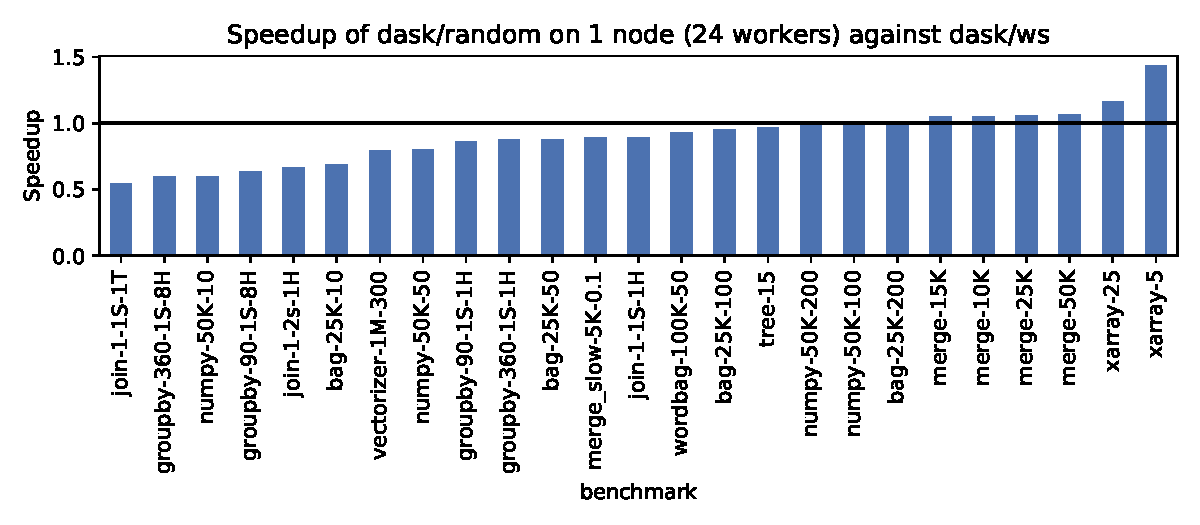
\includegraphics[width=0.9\textwidth]{imgs/rsds/charts/speedup-dask-random-1}
	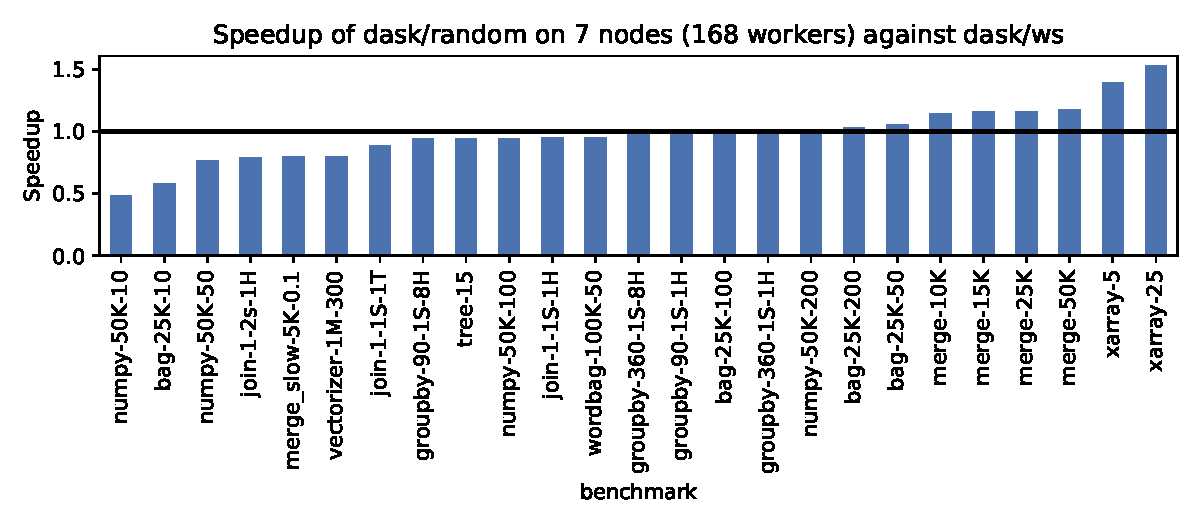
\includegraphics[width=0.9\textwidth]{imgs/rsds/charts/speedup-dask-random-7}
	\caption{Speedup of \dask{}/random scheduler; \dask{}/ws is baseline.}
	\label{fig:dask-ws-vs-random}
\end{figure}

We can observe the results of benchmarks that compare \dask{} using its
baseline work-stealing scheduler vs a completely random scheduler in \Autoref{fig:dask-ws-vs-random}.
Based on these results, it is clear that the random scheduler fares relatively well on both small
and medium sized clusters. At worst, it produces a twice longer makespan, but overall it is quite
close to the performance of the work-stealing scheduler, and in some cases it even outperforms it
with a $1.4\times$ speedup.

If we aggregate the results with a geometric mean, the random scheduler achieves
$88\%$ of the performance of the work-stealing scheduler with a single node,
and $95\%$ with seven nodes. The performance of the random scheduler thus gets
closer to the performance of work-stealing when more workers are used.

The fact that the random scheduler's performance improves with a larger number of nodes is not
surprising. With more nodes, it is easier to fully saturate the potential parallelism contained in
each task graph. Furthermore, a random scheduler produces less network traffic, and has much
smaller computational cost on the server; as we will see in the next experiment, the work-stealing
scheduler's computational cost increases notably when more workers are present.

Furthermore, for certain task graphs, a complex scheduling algorithm might not be needed, and a
random schedule is sufficient to achieve reasonable results. However, all of that combined is still
a rather weak explanation for why is a random scheduler so competitive with the work-stealing
scheduler in \dask{}. In the following experiments, we will show that
\dask{} has considerable runtime overhead, which might introduce a bottleneck
that is more impactful than the effect of the used schedule. In the next section
(\ref{sec:rsds-description}), we will see that with a more efficient runtime and less server
overhead, random schedules will become less competitive.

%There are two effects that explain the reasonable performance of the random scheduler. Firstly, the
%computational complexity of work-stealing scales with the number of available workers. With more
%workers, the work-stealing scheduler has to perform more work to compute where should the tasks be
%computed, and it also generates additional network traffic by sending task stealing messages
%between workers. On the other hand, a random scheduler has a fixed computation cost per task,
%completely independent of the worker count, as it simply chooses a worker randomly, and it also
%sends no additional network messages other than one worker assignment per task. The difference in
%computational overhead between these two schedulers will be examined in more detail in the
%following experiment.

%The second effect is also related to the fact that the random scheduler performs better with more
%workers. Our benchmark set is compute-bound, so if there is a large enough number of workers
%(relative to the number of tasks), it might not be that difficult for the scheduler to saturate all
%the workers, even with a random schedule, as long as the task graph structure is not very
%complicated. Furthermore, if the scheduler wants to utilize all computational power of a cluster
%with many workers, network transfers are less avoidable, which decreases the chance that a random
%scheduler induces an unnecessary data transfer that could have been avoided by a smarter scheduler.

%The results of this experiment suggest that in certain scenarios, a complex scheduling algorithm is
%not needed and a random schedule is sufficient for \dask{}. This shows that the
%scheduler might not be its main bottleneck. We will also examine this in the following experiments.

\subsubsection*{Overhead per task}
\label{sec:dask-overhead-per-task}
We have seen that a random scheduler can be surprisingly competitive with the work-stealing
scheduling implementation in \dask{}. In this experiment, we further examine
this effect by estimating the inner overhead of \dask{} per each executed task.
In order to isolate the effects of the specific executed tasks, and network communication and
worker overhead, we have implemented a special implementation of the \dask{}
worker that we label \emph{zero worker}.

Zero worker is a minimal implementation of the \dask{} worker process, written
in Rust. Its purpose is to simulate a worker with infinite computational speed, infinitely fast
worker-to-worker transfers and zero additional overhead. It actually does not perform any real
computation; when a task is assigned to a zero worker, it immediately returns a message that the
task was finished. It also remembers a set of data-objects that would be placed on the worker in a
normal computation. When a task requires a data object which is not in this list, the worker
immediately sends a message to the server, claiming that the data object was placed on it -- this
simulates an infinitely fast download of data between workers. No actual worker-to-worker
communication is performed in such case.

Zero workers respond to every data object fetch request with a small mocked constant data object.
Such requests come from the server when a client asks for a data object, usually at the end of the
computation. Since there is no worker-to-worker communication when the zero worker is used, fetch
requests never come from other workers.

This idealized worker implementation helps us to understand the fundamental overhead of the
\dask{} runtime, independent of the specific tasks that are being executed.
Note that even though all tasks in this mode are basically the same, the shape and size of the
benchmarked task graph are still important, since they affect the scheduler's performance and also
bookkeeping overhead of the runtime.

\begin{figure}
	\centering
	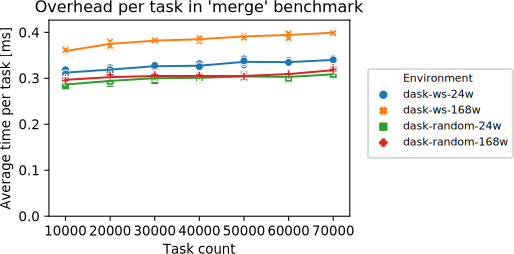
\includegraphics[width=0.5\textwidth]{imgs/rsds/charts/dask-merge-task-scaling}
	\caption{Overhead per task in \dask{} with an increasing number of tasks.}
	\label{fig:dask-merge-task-scaling}
\end{figure}

Using this special mode, we have evaluated the average runtime overhead per each task, which is
calculated as the total makespan divided by the number of tasks in the executed task graph.
\Autoref{fig:dask-merge-task-scaling} shows the average overhead per task for the \texttt{merge}
benchmark, we can see the average overhead per each task (the Y axis), and how it changes with an
increasing number of tasks (X axis). We can observe that the overhead of the random scheduler is
smaller the overhead of the work-stealing scheduler, as expected. We can also see that the overhead
per task increases with an increasing number of tasks, for both schedulers. There is also a
distinct increase of overhead between the overhead with $24$ workers (one
node) and $168$ workers (seven nodes) for the work-stealing scheduler.

\begin{figure}
	\centering
	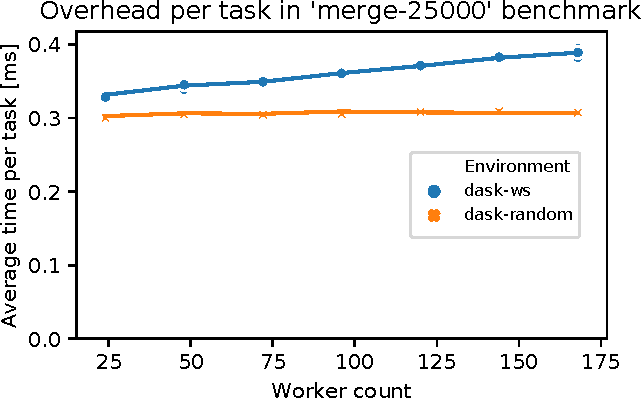
\includegraphics[width=0.5\textwidth]{imgs/rsds/charts/dask-merge-worker-scaling}
	\caption{Overhead per task in \dask{} with an increasing number of workers.}
	\label{fig:dask-merge-worker-scaling}
\end{figure}

This can be examined in more detail in \Autoref{fig:dask-merge-worker-scaling}, which shows how does the
overhead increase when more workers are available. It is clear that the performance of the
work-stealing degrades rapidly when more workers are added to the custer, while the overhead of th
random scheduler stays almost constant, inependent on the number of workers.

The \dask{} manual states that ``Each task suffers about 1ms of overhead. A
small computation and a network roundtrip can complete in less than
10ms.''~\footnote{\url{https://distributed.dask.org/en/latest}}. Our experiment shows that the overhead is less than
$1ms$ for most of our benchmarks.

\begin{figure}
	\centering
	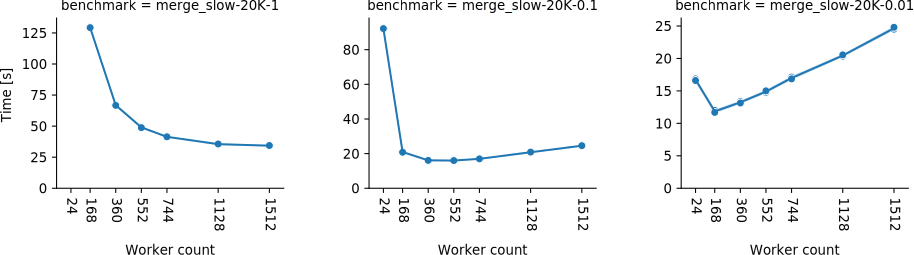
\includegraphics[width=0.9\textwidth]{imgs/rsds/charts/dask-strong-scaling}
	\caption{Strong scaling of \dask{} with different task durations
	($1000ms$, $100ms$ and
	$10ms$).}
	\label{fig:dask-strong-scaling}
\end{figure}

The overhead per task is an important property of the task runtime, since it determines the minimal
duration of a task that is still viable for parallel execution with that runtime. If the duration
of a task is similar or smaller than the overhead of the runtime itself, executing such task with
the runtime will probably not yield any speedup. This is demonstrated in
\Autoref{fig:dask-strong-scaling}, which shows the strong scaling of \dask{} on the
$merge\_slow$ benchmark. The three charts demonstrate its scaling with tasks that take
$1000ms$, $100ms$ and $10ms$ respectively.
With tasks that take a second, \dask{} is able to scale relatively well up to
$1512$ workers. However, when tasks take ten times less time, it only scales up
to around $360$ workers, and when tasks take only $10ms$,
\dask{} scales to around $168$ workers, and adding further
workers makes the makespan longer.

The results of this experiment indicate that the general runtime overhead of
\dask{} mainly grows with an increasing number of tasks, no matter which
scheduler is used. On the other hand, overhead of the work-stealing scheduler grows primarily with
the number of workers. They also show that the minimum duration of tasks executed by
\dask{} should be taken into account, to avoid introducing too much runtime
overhead.

These results also suggest that \dask{} can struggle with a larger number of
workers. This would not be an issue on its own, as every task runtime will have its scaling limit.
However, due to the already mentioned effect of \gls{gil},
\dask{} users might be forced to use more workers than would be otherwise
necessary to achieve reasonable performance. We will examine this in the next experiment.

\subsubsection*{The effect of \gls{gil}}
As noted earlied, the \gls{gil} can have a non-trivial effect on the performance
of Python programs. This can also be seen in \dask{}, where the configuration
of workers might need to be tuned in order to achieve optimal performance.

\begin{figure}
	\centering
	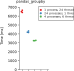
\includegraphics[width=0.3\linewidth]{./imgs/rsds/charts/dask-gil-scaling}
	\caption{Effect of \gls{gil} on the performance of the \emph{pandas\_groupby} benchmark}
	\label{fig:dask-gil-scaling}
\end{figure}

\Autoref{fig:dask-gil-scaling} demonstrates the effect of \gls{gil} on the
\emph{pandas\_groupby} benchmark. We have executed the same benchmark using three
\dask{} worker configurations on a single node. In the default configuration,
with a single worker that uses $24$ threads (one for each core), the pipeline
finishes in approximately $6.5$ seconds. If we instead create a single worker
per each core ($24$ processes, each with a single thread), the performance
improves significantly, by $35\%$! This makes it clear that the
\gls{gil} is a bottleneck in this case, and more \dask{}
workers are needed to improve performance by enabling parallel task execution.

However, it is not so simple as to always use a single \dask{} worker per core.
As we have discovered with our earlier benchmarks, more workers introduce non-negligible overhead
for the \dask{} server. This can be seen from the result of the third
configuration, which uses $4$ \dask{} workers
(processes), each leveraging $6$ threads. This configuration actually
achieves the best performance out of the three tested configurations. It is thus clear that for
some \dask{} workflows, users might need to carefully tune the configuration of
workers to achieve optimal performance.

\subsubsection*{Summary}
Our experiments have shown that \dask{} does not scale optimally to a large
number of workers and it might require manual tuning of worker configuration to achieve the optimal
performance. This lead us to the idea of improving the implementation of the
\dask{} server, in order to reduce its overhead in \gls{hpc}
scenarios.

\section{\rsds{} task runtime}
\label{sec:rsds-description}
In order to examine how much could the performance of \dask{} be improved if we
were able to reduce its runtime overhead, we have developed \rsds{} (Rust \dask{} server), an
open-source drop-in replacement for the \dask{}
server\footnoteurl{https://github.com/it4innovations/rsds}, with the following goals:

\begin{itemize}
	\item Keep backwards compatibility with existing \dask{} programs, so that it can be
	      used to speed up existing workflows. This also enables us to compare the performance of
	      \rsds{} and \dask{} on the benchmarks described in the
	      previous section.
	\item Design an efficient runtime that could scale to \gls{hpc} use-cases, to find a
	      baseline for how much fast could \dask{} become if its overhead was reduced.
	\item Use a modular architecture that would enable easily replacing the implementation of the scheduler,
	      to enable easier experimentation with scheduling algorithms on non-simulated distributed clusters.
\end{itemize}

\subsection*{Architecture}
\rsds{} is implemented in the Rust programming language, which has a minimal
runtime and does not dictate automatic memory management. This reduces the ubiquitous overhead of
reference counting and data indirection present in Python. It also has direct support for
asynchronous \gls{io} and provides strong memory safety guarantees, hence it is
well suited for writing distributed applications.

\begin{figure}[h]
	\centering
	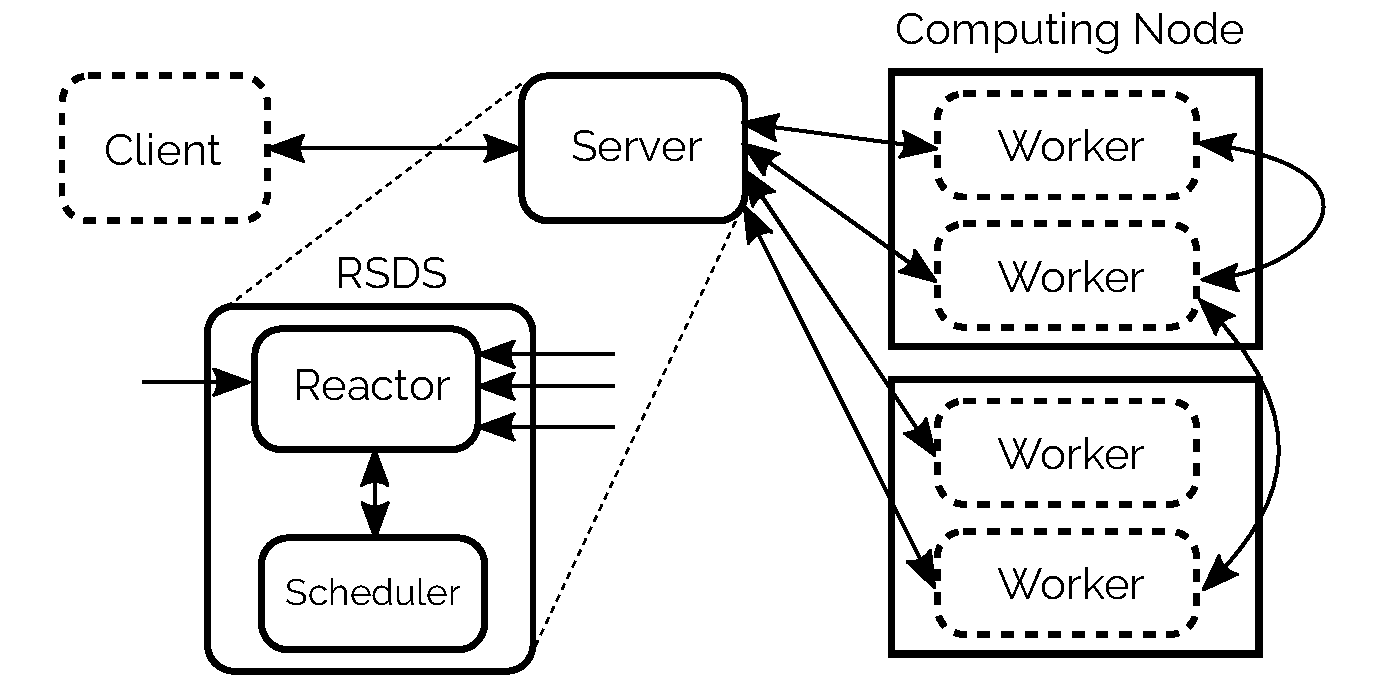
\includegraphics[width=0.8\linewidth]{./imgs/rsds/rsds-architecture}
	\caption{Architecture of \rsds{} (\dask{} components are dashed)}
	\label{fig:rsds-architecture}
\end{figure}

The architecture of \rsds{} is shown in \Autoref{fig:rsds-architecture}. It reuses
the client and worker components from \dask{}, but replaces its server (and
therefore also the scheduler). The main architectural difference between the two implementations is
that \rsds{} separates the server into two parts: \emph{reactor}
and \emph{scheduler}. The reactor manages worker and client connections, maintains
bookkeeping information and translates scheduler assignments into \dask{}
network messages which are then sent to the workers.

The scheduler is a process which receives a task graph and outputs assignments of tasks to workers.
It does not know about network connections, the \dask{} network messages or any
other bookkeeping that is not relevant to scheduling. Since it is isolated, it can be easily
swapped, and therefore it is trivial to experiment with different schedulers in
\rsds{}. Another benefit is that we can easily run the scheduler in a separate
thread to enable concurrent scheduling and runtime management. This is possible because the
scheduler does not share any data structures with the reactor. A disadvantage of this scheme is
that the both the reactor and the scheduler need to build their own task graph, which increases
memory usage, but we have not found this to be a problem in practice.

\subsection*{Compatibility with \dask{}}
The individual \dask{} components communicate together using a custom
communication protocol that contains dozens of different message types. Messages are represented as
dictionaries, where a single field specifies the type of the message and the rest of the fields
contain parameters specific to the given message type.

\dask{} splits messages into multiple parts called \emph{frames}
and serializes each frame with the MessagePack\footnoteurl{https://msgpack.org} binary serialization
format. The messages are split mostly for performance reasons. If a client sends large binary data
to a worker (or vice-versa), the server can deserialize only the first frame containing the message
metadata, and it does not need to further process the binary data, it merely forwards it to the
correct destination. The protocol is designed in such a way that any Python specific objects sent
within the protocol are fully opaque to the server. For example, the server does not need to
understand Python function definitions, it only forwards them from clients to workers, where they
are deserialized and executed. This makes it possible to implement the central server in a
different language than Python.

To retain compatibility with existing \dask{} programs,
\rsds{} must understand this protocol, and be able to both read and also
generate its messages. However, reimplementing the protocol was relatively challenging, because of
two reasons. The first reason is that the protocol is unfortunately mostly
undocumented\footnoteurl{https://github.com/dask/distributed/issues/3357}, and its exact definition depends solely on
\dask{} code that creates the protocol messages ad-hoc in many different source
files and locations. We thus had to reverse-engineer its functionality based on the original
\dask{} source code.

The second reason is that \dask{} makes heavy use of the fact that Python is a
very flexible and dynamic language in its frame encoding scheme. The specific rules of this
encoding grew organically over time and they have become quite complicated and dynamic, as
\dask{} can split messages into frames almost arbitrary ways. Specifically, it
sometimes extracts values out of arbitrary array indices or dictionary keys into a separate frame
during serialization, and then puts them back into the original place during deserialization. The
encoded frame metadata then contains a series of array index and dictionary key accessors. For
example, \verb|[0, "attr1", 1]: <data>| tells the deserializer to put the specified data into the
second element of an array located in the \texttt{"attr1"} key of a dictionary that is
located at the first element of the input array contained within the frame. This dynamic frame
(de)fragmentation is relatively straightforward to perform in a dynamic language like Python, but
it becomes incredibly difficult to handle in a statically-typed language with a strict type system,
such as Rust.

A related issue is that \dask{} sometimes uses a completely different frame
encoding scheme, even for the same message type, which further complicates frame deserialization.
In order to overcome these challenges, we made a small change to the \dask{}
protocol, to make it feasible to implement the server in a statically typed language, which does
not make it trivial to parse the flexible messages generated by \dask{} clients
and workers.

\begin{figure}
	\centering
	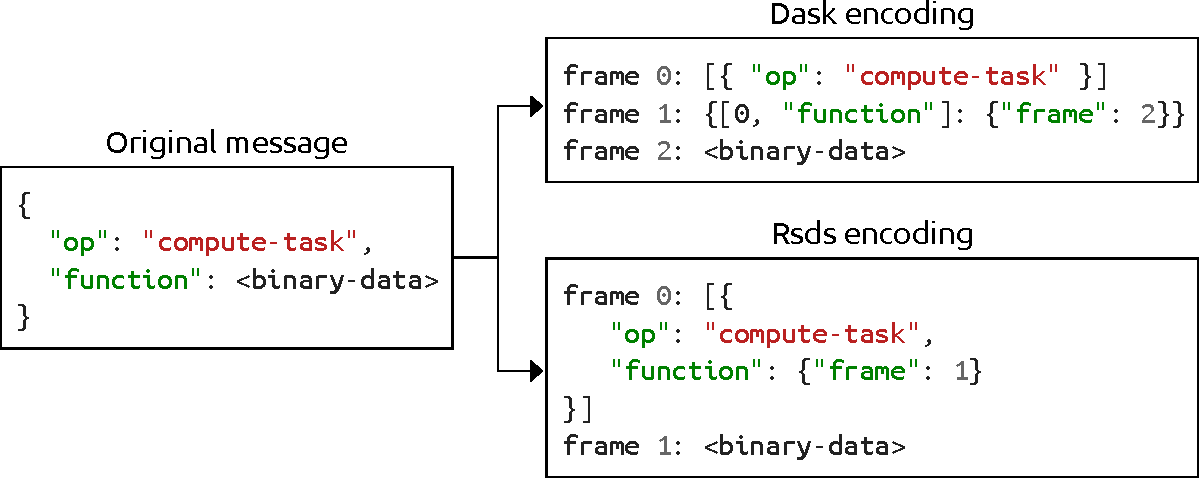
\includegraphics[width=0.9\columnwidth]{./imgs/rsds/frame-encoding}
	\caption{\dask{} message encoding}
	\label{fig:rsds-dask-frame-encoding}
\end{figure}

Our modification changes the dynamic encoding of \dask{} messages into frames.
We have modified it in a way that always keeps the original message structure, so that it is easier
to deserialize. This modification is described in \Autoref{fig:rsds-dask-frame-encoding}, which contains a
simplified scheme that depicts a \dask{} message, and its encoding in
\dask{} and in \rsds{}\footnote{Note that the message and the encoding is depicted using a \gls{json}
notation, for improved readability. In reality, the data is encoded using MsgPack.}. On the
left, we can see the message (dictionary) that we want to serialize, which contains two fields
(\texttt{op} and \texttt{function}). The original
\dask{} encoding, shown in the top right corner, would fragment this dictionary
by removing its \texttt{function} field and moving it to a separate frame. During
deserialization, the field would have to be put back into the original message, transmitted in the
first frame. Our modified encoding, shown in the bottom right corner, instead keeps the original
message structure, but replaces the field that has to be transferred in a separate frame with a
placeholder. During deserialization, the placeholder is replaced with the contents of the second
frame, which is relatively easy to implement in a statically typed language, because it avoids the
need to dynamically change the message structure during deserialization.

This protocol change only modifies low-level message handling, and it is thus fully transparent to
the rest of the code, and spans less than 100 modified lines of \dask{} source
code. Crucially, it has no effect on the functionality of clients, workers and the server, so it
does not require any modifications in \dask{} user programs. Our modified
version of \dask{} is open-source and available
online\footnoteurl{https://github.com/kobzol/distributed/tree/simplified-encoding}. Note that all evaluations presented in this chapter use the
modification described above. We have benchmarked this modification and found that there are no
performance differences in respect to the original \dask{} message encoding.

\rsds{} does not actually implement all \dask{} message
types. Some of them are rarely used, and their implementation would be highly complex, for minimal
gain, and some of them cannot be implemented in a straightforward way in a different language than
Python. For example, Dask contains an \gls{api} that allows clients to run a
Python function on the server, yet this functionality does not have a direct counterpart in a
server implemented in a different programming language. The fact that \rsds{}
is able to execute all the benchmarks described in~\Autoref{sec:rsds-dask-overhead-analysis} demonstrates that it
supports a wide variety of \dask{} programs.

\subsection*{Schedulers}
We have implemented two schedulers in \rsds{}, to allow us comparing its
performance to \dask{} -- a work-stealing scheduler and a completely random
scheduler.

Even though it was not possible to exactly replicate the work-stealing implementation used in
\dask{}, since it is affected by a very large amount of implementation choices
and details, our implementation is inspired by it. However, it is also deliberately kept simple, to
avoid the need to perform extensive hand-tuning of constants and parameters within the scheduler.
Some of the heuristics used by \dask{} were changed, simplified, or dropped in
our implementation. For example \rsds{}, does not estimate average task
durations and does not use any network bandwidth estimates.

The \rsds{} work-stealing scheduler works as follows: when a task becomes ready
(i.e.\ all its inputs are already finished), it is immediately assigned to a worker. The scheduler
chooses a worker where the task may be executed with minimal data transfer costs, while it
deliberately ignores the load of the worker. The load is ignored to speed up the decision in
optimistic situations when there is enough tasks to keep the workers busy. When it is not the case,
it is solved by balancing, which is described below.

When a new task is scheduled or when a task is finished, the scheduler checks if there are nodes
that are under-loaded. In such case, balancing is performed and the scheduler reschedules tasks
from workers with a sufficient number of tasks to under-loaded workers. During rescheduling, the
scheduler simply passes the new scheduling state to the reactor, which performs all of the complex
rescheduling logic. It tries to retract rescheduled tasks from their originally assigned workers.
If retraction succeeds, the task is scheduled to the newly assigned worker. When the retraction
fails, because a task is already running or it has been finished, the scheduler is notified and it
then initiates balancing again, if necessary.

For computing transfer costs, we use a heuristic that takes into account inputs that are already
present on the worker's node, and also inputs that will be eventually present because they are in
transit or they are depended upon by another task assigned to the same worker. Transfer cost is
estimated to be smaller for data transfers between workers residing on the same node.

Our random scheduler mirrors the random scheduler implementation that we have added to
\dask{} -- it assigns a random worker to each task as soon as the task arrives
to the server, using a uniform random distribution. It ignores any other scheduling mechanisms,
such as work-stealing.

\section{Performance comparison of \dask{} and \rsds{}}
\label{sec:rsds-dask-comparison}
We have performed a set of experiments to evaluate how does \rsds{} perform in
comparison to \dask{}. The experiments were performed using the same hardware
and benchmark set that was used for the previous \dask{} experiments, described
in~\Autoref{sec:rsds-dask-overhead-analysis}. Our experiments are structured in the same way as the
\dask{} experiments, they focus on the comparison of the two schedulers, on the
number of workers that each server implementation can scale to, and on their inner overhead per
task. Unless stated explicitly, all experiments use the original \dask{} client
and worker implementations.

\subsection*{Server comparison}

\begin{figure}
	\centering
	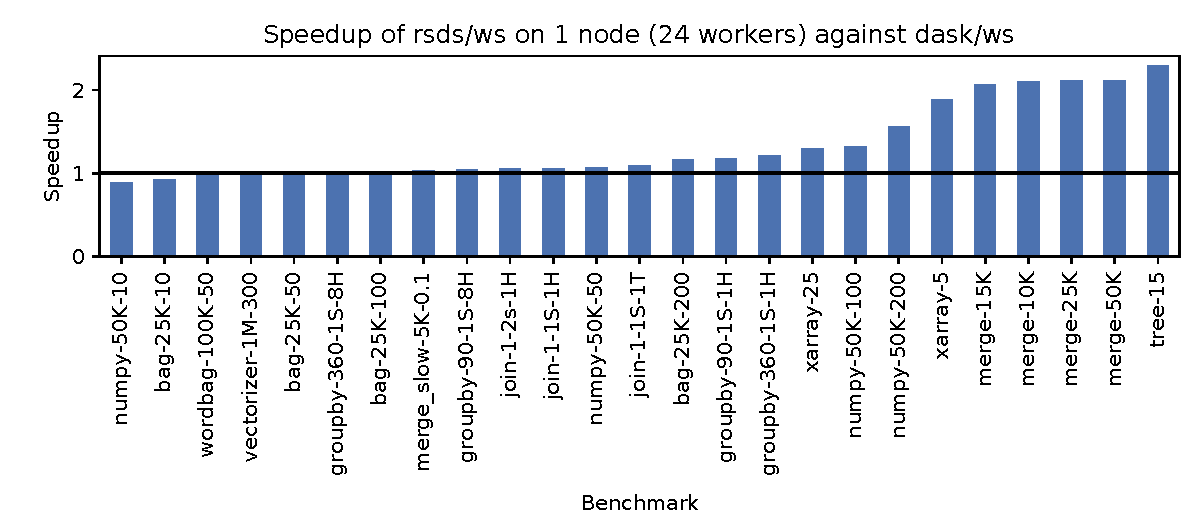
\includegraphics[width=0.8\textwidth]{./imgs/rsds/charts/speedup-rsds-ws-1}
	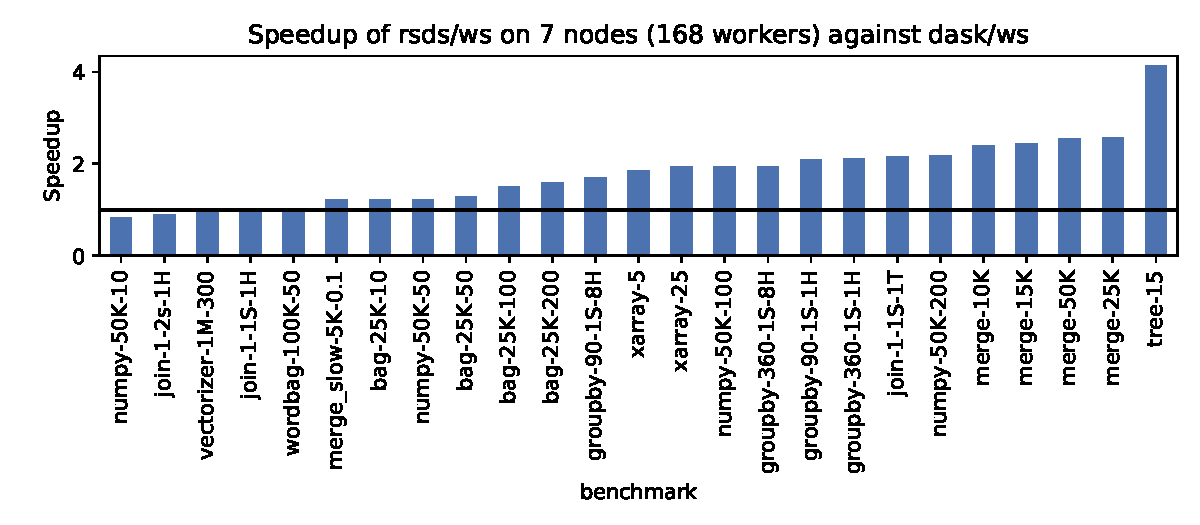
\includegraphics[width=0.8\textwidth]{./imgs/rsds/charts/speedup-rsds-ws-7}
	\caption{Speedup of \rsds{}/ws scheduler; baseline is \dask{}/ws.}
	\label{fig:rsds-dask-ws-all}
\end{figure}

In the first experiment, we have compared the efficiency of the \rsds{} and
\dask{} server implementations on a diverse set of benchmarks, using both the
work-stealing and the random scheduler. The results for the work-stealing schedulers are shown in
\Autoref{fig:rsds-dask-ws-all}. The data confirms our expectation that reducing the overhead of the
server can help improve the makespan of executed task graphs by a non-trivial amount. Even though
\rsds{} uses a much simpler work-stealing scheduler, its more efficient runtime
provides in most cases better performance. This effect is accentuated for a larger cluster with
more workers.

\begin{figure}
	\centering
	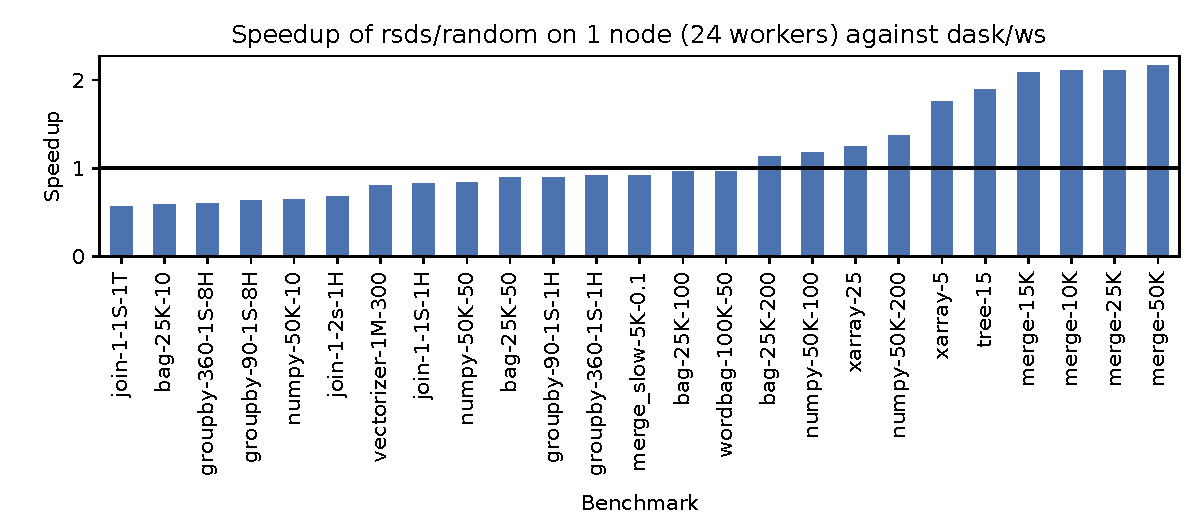
\includegraphics[width=0.8\textwidth]{./imgs/rsds/charts/speedup-rsds-random-1}
	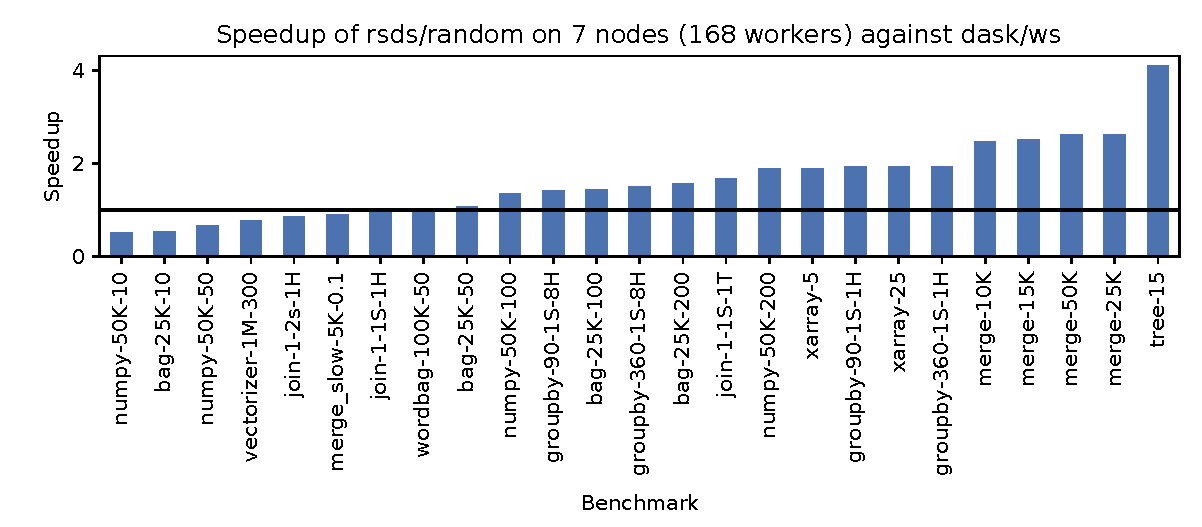
\includegraphics[width=0.8\textwidth]{./imgs/rsds/charts/speedup-rsds-random-7}
	\caption{Speedup of \rsds{}/random scheduler; baseline is \dask{}/ws.}
	\label{fig:rsds-dask-random-all}
\end{figure}

Since the work-stealing implementations of \rsds{} and
\dask{} are not exactly identical, the result above could also be explained by
a difference in scheduling, rather than reduced runtime overhead. To eliminate that possibility, we
have also performed an experiment where we compare \rsds{} using a random
scheduler with \dask{} using its sophihisticated work-stealing scheduler. The
results of this experiment can be seen in \Autoref{fig:rsds-dask-random-all}. They clearly confirm that
the speedup is not caused by \rsds{} having a better scheduler, because even
with a completely random schedule, it is still able to outperform \dask{}. This
serves as an evidence that the improved performance of \rsds{} with
work-stealing is caused by better runtime efficiency, and not by better schedules.

The results of this experiment are summarized in Table~\ref{tab:rsds-geom-mean-speedup}, which shows the
geometrical mean of speedup of the tested \rsds{} configurations, over a
baseline using the \dask{} server with the work-stealing scheduler. The table
also contains the results of the \dask{} server with a random scheduler, to
provide a more complete picture. Even with the random scheduler, \rsds{} is on
average faster than \dask{} using work-stealing. With more workers, this effect
is further increased.

\setlength{\tabcolsep}{5pt}
\begin{table}
	\caption{Geometric mean of speedup over the \dask{}/ws baseline}
	\centering
	\label{tab:rsds-geom-mean-speedup}
	\begin{tabular}{c|c|r|r|r}
		\textbf{Server} & \textbf{Scheduler} & \textbf{Node count} & \textbf{Worker	count} &
		\textbf{Speedup}                                                                                 \\
		\midrule
		dask            & random             & 1                   & 24                   & $0.88\times$ \\
		rsds            & random             & 1                   & 24                   & $1.04\times$ \\
		rsds            & ws                 & 1                   & 24                   & $1.28\times$ \\
		dask            & random             & 7                   & 168                  & $0.95\times$ \\
		rsds            & random             & 7                   & 168                  & $1.41\times$ \\
		rsds            & ws                 & 7                   & 168                  & $1.66\times$ \\
	\end{tabular}
\end{table}

In~\Autoref{sec:rsds-dask-overhead-analysis}, it was noted that the random scheduler used in
\dask{} was quite competitive with the work-stealing scheduler implementation.
Our hypothesis was that this phenomenon is reinforced by the runtime overhead of
\dask{}. To test this hypothesis, we have also compared the performance of the
random scheduler in \rsds{} vs its work-stealing implementation. The results
can be observed in \Autoref{fig:rsds-random-baseline}. We can see that in the case of
\rsds{}, the random scheduler is less competitive (cf.~\Autoref{fig:dask-ws-vs-random}
and~\Autoref{fig:rsds-random-baseline}), and does not significantly outperform work-stealing in any of
the benchmarked cases. This suggests that with a more reasonable runtime overhead of the server, a
work-stealing scheduler is strictly better than a random scheduler, which is a much more intuitive
result.

\begin{figure}
	\centering
	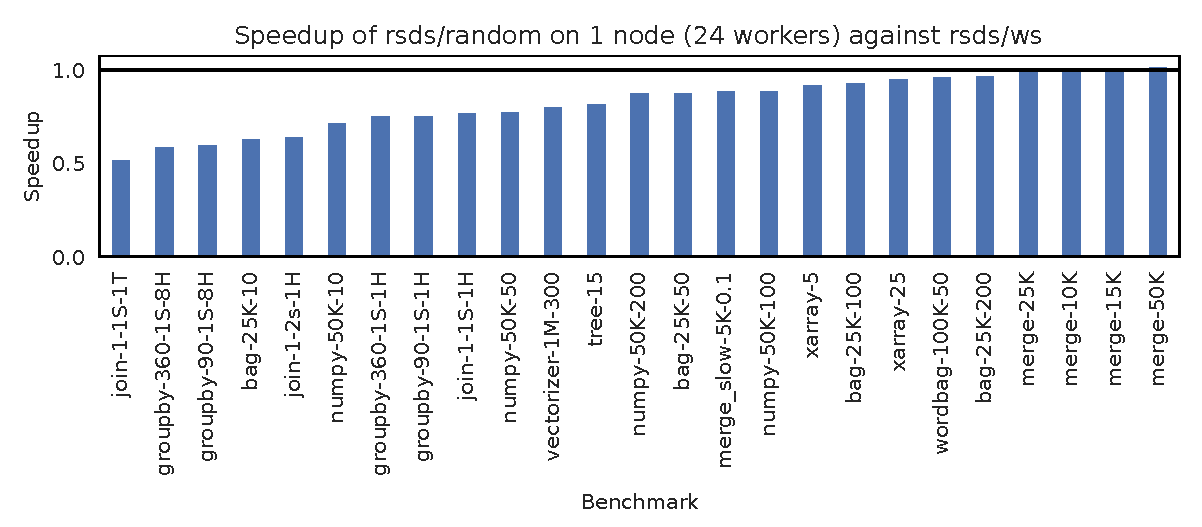
\includegraphics[width=0.9\textwidth]{./imgs/rsds/charts/speedup-rsds-random-1-baseline-rsds-ws}
	\caption{Speedup of \rsds{}/random scheduler; baseline is \rsds{}/ws.}
	\label{fig:rsds-random-baseline}
\end{figure}

To provide a clearer comparison of the random scheduler results,
Table~\ref{tab:rsds-random-geom-mean-speedup} shows the
geometric mean of speedup of the random scheduler, compared to a work-stealing scheduler baseline
of a corresponding server implementation. It is clear from the results that in
\rsds{}, the random scheduler is less performant (relative to its work-stealing
counterpart) than in \dask{}.

\setlength{\tabcolsep}{5pt}
\begin{table}
	\caption{Geometric mean of speedup for random schedulers}
	\centering
	\label{tab:rsds-random-geom-mean-speedup}
	\begin{tabular}{c|c|r|r|r|r}
		\textbf{Server}      & \textbf{Scheduler} & \textbf{Baseline} & \textbf{Node count} &
		\textbf{Worker	count} & \textbf{Speedup}                                                   \\
		\midrule
		dask                 & random             & dask/ws           & 1                   & 24
		                     & $0.88\times$                                                       \\
		rsds                 & random             & rsds/ws           & 1                   & 24
		                     & $0.82\times$                                                       \\
		dask                 & random             & dask/ws           & 7                   & 168
		                     & $0.95\times$                                                       \\
		rsds                 & random             & rsds/ws           & 7                   & 168
		                     & $0.85\times$                                                       \\
	\end{tabular}
\end{table}

\subsection*{Scaling comparison}
One of the motivations for implementing \rsds{} was to improve the performance
of \dask{} workflows in \gls{hpc} scenarios. In these
use-cases, it is important for the runtime to scale to a large amount of workers, which can be
provided by an \gls{hpc} cluster. We have designed an experiment which tests the
strong scaling of both server implementations on several cluster sizes, ranging from
$1$ node ($24$ workers) to $63$
nodes ($1512$ workers). The default, work-stealing scheduler was used for both
server implementations.

\begin{figure}[h]
	\centering
	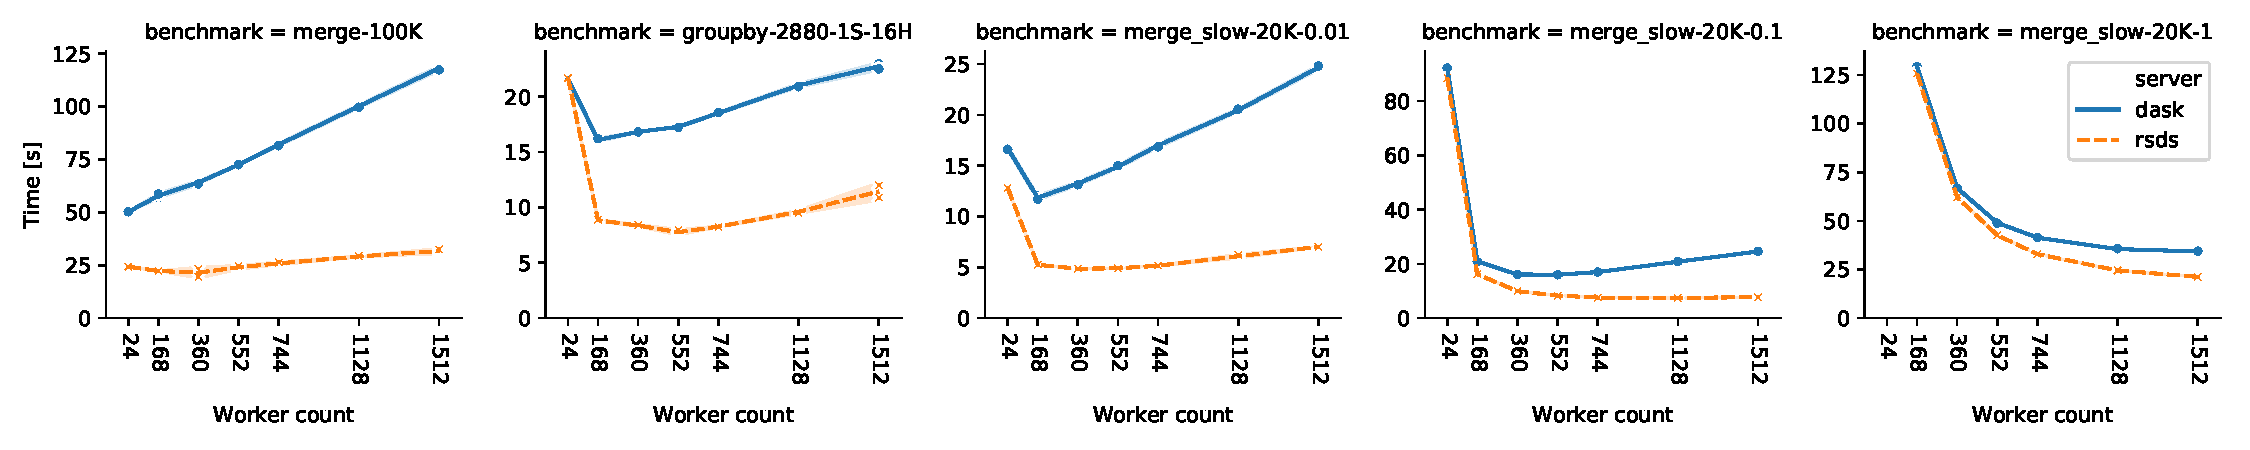
\includegraphics[width=0.8\textwidth]{./imgs/rsds/charts/rsds-dask-scaling}
	\caption{Strong scaling of \rsds{} vs \dask{} on selected task graphs}
	\label{fig:rsds-dask-scaling}
\end{figure}

The results of this experiment are shown in \Autoref{fig:rsds-dask-scaling}. The first examined task
graph is \texttt{merge-100K}, which executes hundred thousand trivial, almost instant
tasks. It is an adversarial case for a scheduler, as the tasks are short and thus the overhead of
scheduling and network transfers will overcome most parallelism gains. Therefore, increasing the
amount of workers will probably not provide a large speedup for this task graph. However, it should
ideally not slow down the computation to a large extent. We can see that
\rsds{} scales up to $15$ nodes
($360$ workers). This is caused by the fact that the cost associated with
worker management and work-stealing increases with an increasing number of workers, and from some
point it starts to dominate, because the tasks are too short. However, \dask{}
fares much worse. It is twice slower when compared to \rsds{} with a single
worker node, but four times slower with $63$ nodes
($1512$ workers). Here we can see that the inner overhead of
\dask{} adds up, and its performance is reduced significantly with each
additional worker node. On the other hand, with \rsds{}, the total makespan
stays relatively constant, even after it stops scaling.

The next tested benchmark was \texttt{groupby-2880-1S-16H}, which computes an analysis of table data
using a task graph automatically generated by \dask{}, using the
\texttt{DataFrame} \gls{api} inspired by the \texttt{pandas}
interface. This task graph provides many opportunities for parallelization, as the individual tasks
work on a subset of rows and thus have more computational density compared to the
\texttt{merge} task graph. However, Table~\ref{tab:dask-graph-properties} shows that the
average computation time is still only around $10ms$, while the average task
output is $1 MiB$. This benchmark thus produces considerable network traffic.
While both \dask{} and \rsds{} have identical performance
with a single worker node, \dask{} stops scaling at $7$
nodes and further its performance degrades and eventually becomes slower than the single node case.
\rsds{} scales up to $23$ worker nodes, hence it is able
to utilize three times more workers. With more worker nodes, the performance of
\rsds{} also degrades, as the network communication caused by task output
transfers and work-stealing messages starts to dominate the overall execution time. In this case,
\dask{} and \rsds{} follow a very similar scaling pattern,
however, in absolute terms, the makespans are twice shorter with \rsds{}, and it does not become
slower with more workers than with just a single worker.

The third examined task graph is \texttt{merge\_slow-20K}, which executes twenty thousand tasks,
where each task has a fixed duration, specified by a parameter (note that the
\texttt{merge} and \texttt{merge\_slow} benchmarks have the exact same task
graph shape, the only difference is the duration of each task). We have benchmarked three variants
of this task graph, with $0.01$, $0.1$ and
$1$ second tasks, same as for the previous similar experiment that we have
performed with \dask{} only. This gives us a better idea of the task
granularity required for \dask{} and \rsds{} to scale
effectively. With $10$ millisecond tasks, \dask{} scales
to $7$ workers and then its performance follows a similar shape as for
\texttt{merge-100K}. \rsds{} stops scaling at
$15$ nodes, then its performance drops slightly with more added nodes. With
$100$ millisecond tasks, \rsds{} is able to scale up to
$47$ worker nodes ($1128$ workers), from that point on
its performance stagnates. \dask{} scales only up to $23$
worker nodes, then the makespan again starts to increase when additional workers are added. For the
last task graph, with one second tasks, both \rsds{} and
\dask{} scale up to $63$ nodes
($1512$ workers). However, \rsds{} is consistently faster
on all cluster sizes, and its performance in respect to \dask{} increases with
added worker nodes; it is $1.03\times$ faster than \dask{} with
$7$ nodes and $1.6\times$ faster with
$63$ nodes.

In general, \rsds{} is able to scale to a larger number of workers than
\dask{}, thanks to its reduced runtime overhead. Furthermore, it is also able
to keep its performance relatively steady with an increasing number of workers, even after it stops
scaling, even for short tasks.

\subsubsection*{Overhead per task}
In~\Autoref{sec:dask-overhead-per-task}, we have seen that the average overhead of
\dask{} for each task is around $0.3ms$. In this experiment,
we have measured the per-task overhead of \rsds{}, so that we could qualify how
much was its overhead reduced, relative to the baseline. All the benchmarks in this experiment were
performed with the \emph{zero worker} implementation.

\begin{figure}
	\centering
	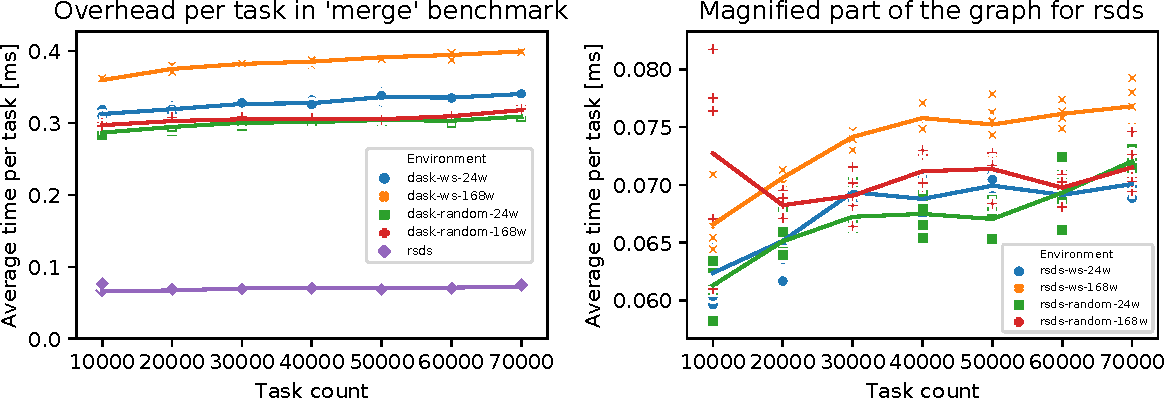
\includegraphics[width=0.8\textwidth]{./imgs/rsds/charts/rsds-merge-task-scaling}
	\caption{Overhead per task for \rsds{} and \dask{} with an
	increasing number of tasks.}
	\label{fig:rsds-merge-task-scaling}
\end{figure}

We have performed the same experiment as with \dask{}, to calculate the
per-task overhead on the \emph{merge} benchmark. \Autoref{fig:rsds-merge-task-scaling} shows
how does the per-task overhead change for larger task graphs. From the chart on the left side, we
can see that the per-task overhead of \rsds{} is approximately
$3-4$ times smaller than the overhead of \dask{}. From
this chart, it looks like its overhead stays constant with an increasing number of tasks, yet when
we zoom in on the section containing \rsds{} results (which we can see in the
chart on the right side), we can observe a similar pattern that we see for
\dask{} -- the overhead of the work-stealing scheduler increases slightly with
more tasks, and the work-stealing scheduler has a larger overhead than the random scheduler, in
general. However, it happens on a much smaller absolute scale than with
\dask{}.

\begin{figure}
	\centering
	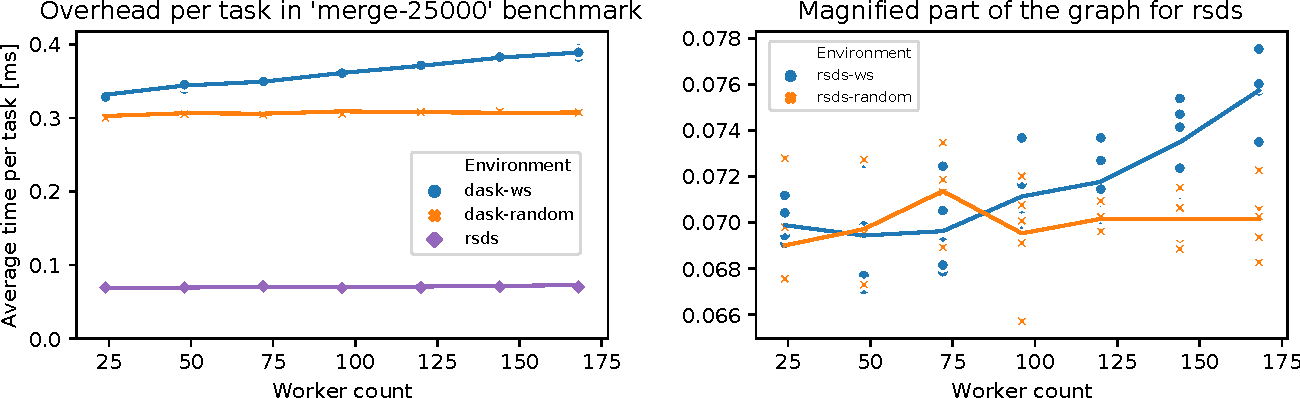
\includegraphics[width=0.8\textwidth]{./imgs/rsds/charts/rsds-merge-worker-scaling}
	\caption{Overhead per task for \rsds{} and \dask{} with an
	increasing number of workers.}
	\label{fig:rsds-merge-worker-scaling}
\end{figure}

\Autoref{fig:rsds-merge-worker-scaling} depicts the results of per-task overhead for an increasing
number of workers. The results are almost identical, the overhead of \rsds{} is
several times smaller than with \dask{}, and it increases for the work-stealing
scheduler slightly with more added workers. Athough this increase is so small that it is almost
negligible, at least for the benchmarked number of workers.

\begin{figure}
	\centering
	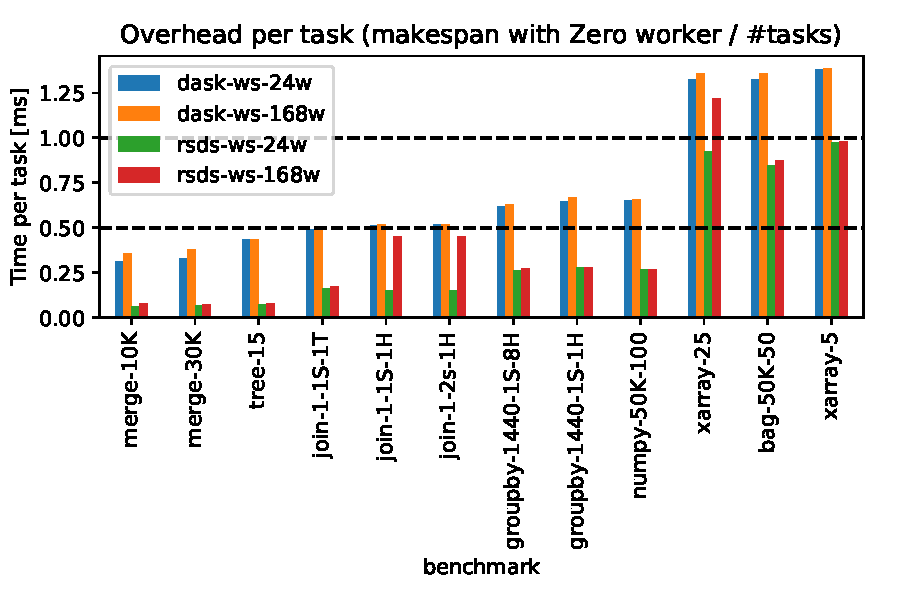
\includegraphics[width=0.8\columnwidth]{./imgs/rsds/charts/rsds-dask-overhead-all}
	\caption{Overhead per task for various cluster sizes and benchmarks}
	\label{fig:rsds-dask-overhead-all}
\end{figure}

In order to confirm that the per-task overhead results from the \emph{merge}
benchmark generalize to other benchmarks, we have also performed a similar experiment for several
other task graphs. The results of this experiment are shown in Figure~\ref{fig:rsds-dask-overhead-all}.
We can see that the overhead for the \emph{merge} benchmark is on the lower end of
the spectrum, and it reaches up to $1.25$ ms for some other benchmarks. The
results show that the per-task overhead of \rsds{} is always smaller then the
overhead of \dask{}, however the difference is not that large for the
\emph{xarray} and \emph{bag} benchmarks.

\begin{figure}
	\centering
	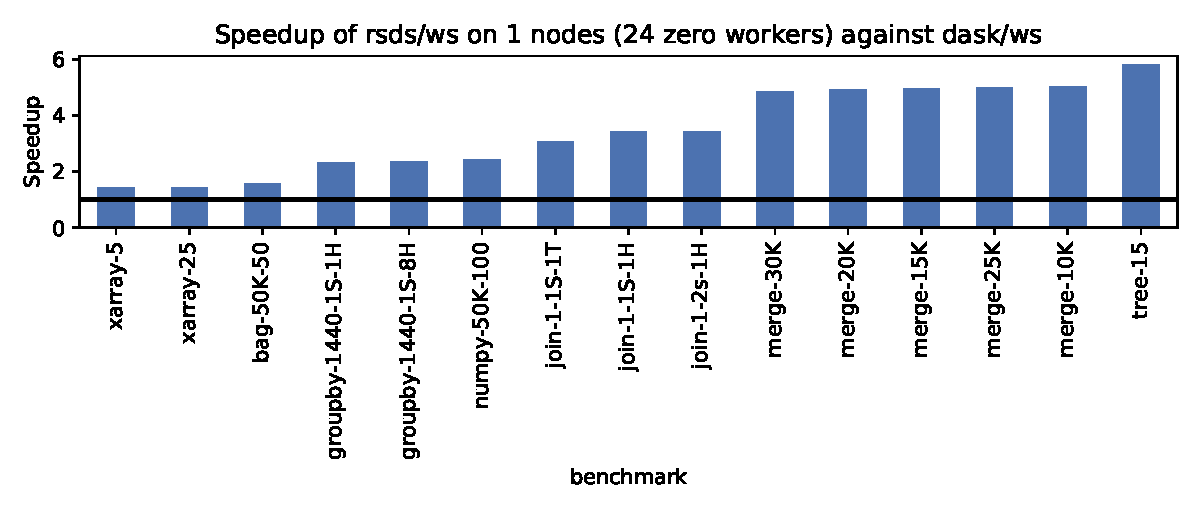
\includegraphics[width=0.9\textwidth]{./imgs/rsds/charts/speedup-zw-rsds-ws-1}
	\caption{Speedup of \rsds{}/ws over \dask{}/ws with the zero worker
	implementation}
	\label{fig:rsds-zero-worker-speedup}
\end{figure}

To evaluate the end-to-end effect of overhead on task graph makespan, we have executed several
benchmarks with the \emph{zero worker} implementation, and compared their overall
makespan, for both \dask{} and \rsds{}. Note that we could
not have evaluated all the benchmarks with the zero worker mode, since some of the task graphs
depend on the actual computed contents of data objects generated by tasks, however the zero worker
implementation does not execute tasks, and it is thus not able to generate the correct data. The
results of this benchmark can be found in \Autoref{fig:rsds-zero-worker-speedup}. In all the tested
benchmarks, \rsds{} produced shorter makespans than
\dask{}; in some cases it was up to six times faster. This speedup is larger
than with the standard worker implementation; this shows that if the overhead of the worker was
further reduced, \rsds{} could futher improve its performance advantage over
\dask{}. In other words, \rsds{} would benefit more from a
faster worker implementation than the \dask{} server could.

All these experiments have shown that \rsds{} exhibits similar performance
behavior and scaling patterns as \dask{}, which is not surprising, given that
it reuses its client and worker implementations. However, the most important result is that in
absolute terms, it tends to be faster than \dask{} across various task graphs
and cluster sizes, even though it uses a much simpler scheduling algorithm, which suggests
that optimizing the runtime overhead of the \dask{} server is a more worthwhile effort than
improving its scheduling algorithm.

The overall overhead present in the whole \rsds{} cluster
could be further reduced e.g.\ by also implementing the worker (or even the client) in another
language than Python, however that would probably make it quite challenging to keep backwards
compatibility with existing \dask{} programs.

\section*{Summary}
We have analyzed the performance of the \dask{} task runtime on a set of
diverse benchmarks in an \gls{hpc} setting. Our analysis has demonstrated that
\dask{} is heavily bottlenecked by the runtime overhead of its Python
implementation, and also by other aspects related to the usage of Python, notably the presence of
the \gls{gil}. This suggests that further optimizations should focus mainly on
the overhead of its server, rather than its scheduler, as even a completely random scheduler is
able to achieve quite reasonable performance, since the schedule is not the primary bottleneck, at
least in certain cases.

To improve the performance of \dask{} workflows, we have developed
\rsds{}, an open-source drop-in replacement for the \dask{}
server. It was built from the ground up with a focus on runtime
efficiency and scheduler modularity, but at the same time we have designed it to be compatible with
the original \dask{} protocol, which means that it is backwards-compatible with
existing \dask{} programs, and can be used to speed them up.

We have performed a series of experiments where we have compared the performance of
\rsds{} vs \dask{}. The results of our experiments indicate
that optimizing the runtime is definitely a worthy effort to pursuit, as
\rsds{} has been able to outperform \dask{} in various
scenarios, even though it uses a much simpler work-stealing scheduling algorithm.

After we had an indication that \rsds{} can be used to improve the efficiency
of existing \dask{} workflows, we have contacted the authors and maintainers of
\dask{}, and discussed the \rsds{} approach with
them\footnoteurl{https://github.com/dask/distributed/issues/3139}\footnoteurl{https://github.com/dask/distributed/issues/3783}\footnoteurl{https://github.com/dask/distributed/issues/3872}. Some of its
ideas have been since adapted in the \dask{} project and led to improving its
performance.


	\chapter{Task graph meta-scheduling}
	\label{ch:hyperqueue}
	%TODO: fix P(Rwid)
%TODO: fractional resources experiment
%TODO: ergonomics/efficiency for meta-scheduling design and resources
%TODO: SOTA for resource management
The previous two chapters focused primarily on the performance aspects of task graph execution, by
examining various task scheduling algorithms and also bottlenecks that can limit the scalability of
existing task runtimes. However, while performance is naturally crucial for
\gls{hpc}, it should not be the only factor to focus on. \Autoref{ch:sota}
discussed several other challenges affecting \gls{hpc} task graphs that are related
to the second main focus of this thesis, namely the ergonomics of task graph execution.

This chapter deals with these ergonomic challenges through a meta-scheduling design that provides a
set of guiding principles for implementing task runtimes. It takes into account heterogeneous
resource management, fault tolerance, dynamic load balancing, interaction with allocation managers
and other aspects required to enable effortless execution of task graphs on supercomputers.

This design is then combined with the performance-related insights into task scheduling and
minimizing runtime overhead presented in Chapters~\ref{ch:estee}
and~\ref{ch:rsds} in an implementation of an \gls{hpc}-tailored task
runtime called \hyperqueue{}. This task runtime was created with the goal of enabling
transparent, ergonomic and efficient execution of task graphs on \gls{hpc} clusters.
It is the culmination of the research and work presented in this thesis, which was made possible
thanks to the experience gained from our work on \estee{} and
\rsds{} and also from interacting with many \gls{hpc} workflows and
use-cases over the course of several years.

The work presented in this chapter makes the following contributions:
\begin{enumerate}[itemsep=0pt,topsep=5pt]
	\item We propose a meta-scheduling design that provides a unified method for executing tasks in the
	      presence of allocation managers and allows load balancing across different allocations, by
	      disentangling the definition of tasks and the hardware resources that executes them.
	\item We describe a novel resource management scheme designed to improve hardware utilization of
	      heterogeneous clusters.
	\item We provide an implementation of the meta-scheduling and resource management design in
	      \hyperqueue{}, a task runtime that enables ergonomic and efficient execution of task graphs
	      on \gls{hpc} clusters.
	\item We evaluate the performance, scalability and achieved hardware utilization of task graphs executed
	      using \hyperqueue{} on several benchmarks and use-cases.
\end{enumerate}

This chapter first introduces the proposed general meta-scheduling design and also several concepts
useful for improving the utilization of heterogeneous resources. Then it describes the architecture
of \hyperqueue{}, which implements the proposed design, and discusses how its features
alleviate the challenges described in~\Autoref{ch:sota}. Finally, it presents several
use-cases where \hyperqueue{} was successfully used, provides a performance analysis of
\hyperqueue{} on various use-cases and stress tests and compares it with state-of-the-art
meta-scheduling task runtimes.

We have described the design and key ideas of \hyperqueue{} in
\emph{HyperQueue: efficient and ergonomic task graphs on HPC clusters}~\cite{hyperqueue}. The architecture of \hyperqueue{}
presented in this chapter was adapted from this publication.

\workshare{I have collaborated on this work with Ada Böhm; we have both contributed to it equally. I am the
sole author of the design and implementation of the automatic allocator
component, and I have also significantly contributed to the design and implementation of most remaining parts
of \hyperqueue{}. I have designed and performed all the experiments described in this
chapter. While Ada and I are the primary contributors to \hyperqueue{}, it should be noted that other people have also contributed to it, as its development is a team effort. Source code contribution statistics for
\hyperqueue{} can be found on GitHub\footnoteurl{https://github.com/it4innovations/hyperqueue/graphs/contributors}.}

\section{Meta-scheduling design}
This section describes a design for executing task graphs that aims to alleviate the challenges
described in~\Autoref{ch:sota}. It consists of a set of general guidelines that should help
drive the design of task runtimes so that they will be able to resolve these challenges. Note that
this section focuses on general principles that do not depend so much on a specific implementation.
There are some task runtime aspects, such as simple deployment or high runtime efficiency, that
have to be resolved with specific implementation choices rather than general principles. These will
be mentioned in a following section that will detail the implementation of the
\hyperqueue{} task runtime, which implements the described meta-scheduling design.

The primary challenge that affects the simplicity of task graph execution on
\gls{hpc} clusters is the presence of an allocation manager, because it forms a
barrier; on such clusters, it is not possible to compute anything at all without interacting with
allocations. In order for task graph execution to become truly ergonomic, it is the first and
foremost challenge that needs to be resolved. It is also tied to most of the other mentioned
challenges; heterogeneous resource requirements, fault tolerance and efficient hardware utilization
on supercomputers are all affected by the way the task runtime handles allocations. It will thus be
the main focus of the described guidelines.

\Autoref{challenge:allocation-manager} has described several approaches that can be used to map tasks to
allocations, as well as their various shortcomings. Due to the limits imposed by allocation
managers, it might be necessary to partition task graphs into multiple subgraphs in order to fit
them within an allocation, which can be challenging. Furthermore, it can result in non-optimal
usage of hardware resources, because tasks from (sub)graphs submitted in separate allocations will
only be load balanced within their own allocation rather than also across different allocations.

It is important to note what is uniquely challenging about the interaction with allocations. The
fact that the computation needs to go through a queue is not an issue by itself, as we are dealing
with batch processing anyway. Therefore, some form of a delay between submitting the task graph and
receiving the results is expected, even if we did not have to submit allocations at all.

The main issue of allocations is that they strictly tie together two separate aspects;
\emph{what} the user wants to compute (the computation performed once the allocation
starts) and \emph{where} should the computation take place (specific hardware resources
and computational nodes reserved for the allocation). As was already described previously, both of
these things have to be specified together in an allocation. This is a very inflexible design because of
several reasons:

\begin{itemize}[itemsep=0pt]
	\item The user needs to consider both aspects at the same time. Ultimately, the main thing that the user
	      cares about is what they want to compute. With allocations, they also need to think about specific
	      hardware resources that should be allocated for computing their tasks, and how should tasks be
	      mapped to these resources, which can be challenging.
	\item Hardware resources are allocated for the whole duration of the allocation. This can result in
	      inefficient resource usage, especially for heterogeneous task graphs that consist of many types of
	      tasks that use different resources. In situations where not all resources can be used at the same
	      time, some of the resources can unnecessarily remain idle.
	\item The amount of used resources has to be decided up front; new hardware resources cannot be added or
	      removed from existing allocations. Apart from the potential resource waste, this can also limit
	      load balancing. If load balancing only happens within (and not across) allocations, then resources
	      from different allocations cannot be pooled together to make the task graph execution faster, and
	      users also cannot easily add new hardware resources during the computation of a task graph.
	\item Granularity of the allocated resources might not match the granularity of tasks. Unless the
	      allocation manager supports very fine-grained allocations (e.g.\ on the level of individual
	      \gls{cpu} cores rather than whole computational nodes), there can be a large gap
	      between the resources required by a task graph and the resources provided to an individual
	      allocation. This can again lead to resources sitting idle.
	\item Binding computation with specific hardware resources up front complicates handling task failures.
	      When the user submits thousands of tasks on a specific set of hardware resources and some of these
	      tasks fail, the user might need to create a new allocation to recompute the failed tasks. This
	      requires once again figuring out a new set of hardware resources that should be requested, as the
	      original resources might not be a good fit for just a subset of the original computation. A
	      fault-tolerant design would ideally allow recomputing tasks on any compatible hardware resource
	      transparently, which is incompatible with forcing computations and resources to be defined
	      together.
\end{itemize}

As an aside, it is interesting to note that some of these challenges uniquely affect task graphs,
and in general programming models that are different from the traditional ways of defining
\gls{hpc} computations. Consider a distributed application implemented using
\gls{mpi}, which has historically been a common way of defining computations on
supercomputers. \gls{mpi} applications typically assume that they will run on a set
of computational nodes for a relatively long duration (hours or even days). This set of nodes
(corresponding to \gls{mpi} processes) usually does not change during the
computation; it is not trivial to add new processes, and if some of the processes crash, it
typically leads to the whole computation being aborted, as fault tolerance is not a default
property of \gls{mpi} applications~\cite{fault_tolerant_mpi}.

These properties of \gls{mpi} applications are similar to the mentioned properties of
allocations, so they fit together well; using allocations to execute them is relatively
straightforward. In fact, it is clear that the allocation model itself was designed with
\gls{mpi}-like use-cases in mind. Therefore, it is not very surprising that the
concept of allocations is not a good match for programming models that are very different from
\gls{mpi}, such as task-based workflows.

In order to remove this problematic aspect of allocations, the key idea of the proposed
meta-scheduling design is to completely disentangle the definition of what the user wants to
compute (tasks) from the hardware resources where the computation should take place (computational
nodes, \gls{cpu} cores, etc.). By separating these two concerns, we enable users to
focus on what they care about the most (their task graphs), instead of having to think about
mapping tasks to allocations and graph partitioning.

In order to disentangle these two concepts, we have to rethink what kind of computation is
submitted in allocations. Instead of making allocations execute tasks or task graphs directly, they
should execute generic computational providers, which will then be dynamically assigned work (tasks
to execute) based on the current computational load. This both improves the achievable hardware
utilization and simplifies the allocation submission process. The following principles describe a
meta-scheduling approach based on this idea, along with several additional guidelines designed for
ergonomic task execution.

\begin{description}[wide=0pt]
	\item[Task runtime runs outside of allocations] In order to allow fully dynamic load balancing, the task runtime should not be tied to a specific
		allocation. Instead, it should run at some persistent location of the cluster (e.g.\ on a login
		node). This enables users to submit tasks to it independently of allocations, which is a crucial
		property. This removes the need to decide which tasks should be computed on which concrete hardware
		resources and in which allocations up front. It can also help improve hardware utilization, because
		it provides the task runtime the possibility to load balance tasks across all active allocations.

		This is where the term \emph{meta-scheduling} comes in; the essence of the idea is to use a task
		runtime as a sort of a high-level scheduler on top of an allocation manager. Instead of forcing
		users to think in terms of allocations, they can submit task graphs in the same way they would on a
		system that is not supervised by allocation managers and let the task runtime automatically decide
		in which allocation a task should be executed.

		With this approach, the task runtime will most likely run in an environment that is shared with
		other users of the cluster, rather than being executed inside secured and isolated allocations. It
		should thus offer its users an option to encrypt its communication to avoid other users of the
		cluster reading sensitive data (e.g.\ task outputs) sent from workers.
	\item[Allocations are uniform] Even with the task runtime running outside an allocation, it is still necessary to submit
		\emph{some} allocations to provide hardware resources that will actually execute tasks.
		Instead of defining specific tasks that should be computed within an allocation, allocations should
		execute a generic computational provider (worker) that will be assigned tasks to execute
		dynamically by the task runtime. This assignment can happen e.g.\ by a centralized component
		pushing tasks to workers over the network, or by the workers pulling work from a queue or a
		distributed database.

		With this approach, allocations become trivial and completely uniform, because they all have the
		same structure; each allocation simply starts a (set of) computational provider(s). This makes it
		much easier for users to submit allocations. Instead of thinking about how to partition their task
		graphs, users simply decide how many computational resources they want to spend at any given moment
		and then they start the corresponding number of allocations.
	\item[Allocations are submittable automatically] A corollary of the previous principle is that it becomes possible to submit allocations fully
		automatically by the task runtime. It can use its knowledge of the current computational load to
		submit workers whose resources would help execute tasks that are currently waiting for hardware
		resources. This saves users from performing a laborious manual process (allocation submission) and
		can further help improve hardware utilization, since the task runtime can use its knowledge to
		dynamically increase and decrease the number of active workers.
	\item[Failed tasks are retried automatically] Once allocations become generic computational providers, their lifetime is no longer bound to a
		specific set of tasks. And since allocations often end abruptly, they might disappear in the midst
		of a task being computed. This is not a failure of the task per se; it is a mostly unavoidable
		consequence of allocations being transient. Such tasks should thus be automatically reassigned by
		the task runtime to a different worker without the user's intervention, in order to ensure
		uninterrupted execution of the task graph.

		The fact that the task runtime resides outside of allocations further facilitates fault tolerance,
		because an allocation failure will not affect the state of tasks stored in the task runtime. In
		order to also be resilient against e.g.\ login node failures, the task runtime should be able to
		restore its state from persistent storage (e.g.\ a filesystem or a database).
	\item[Dependencies are independent of allocations] The allocation manager should not act as a task runtime and thus it should not handle dependencies
		between tasks. These should be expressed solely on the level of the task runtime itself and they
		should be fully independent of allocations. This approach also facilitates execution of the task
		runtime on a local computer, where there most likely will not be any allocation manager available.
	\item[Tasks are paired with workers using abstract resources] The first two principles described above separate the two core pillars of task graph execution; the
		definition of the task graph and the provisioning of hardware resources. However, it is in fact
		required to somehow tie these two aspects together, because tasks can have resource requirements
		that constraint the environment in which they can be executed.

		We saw that submitting tasks directly as allocations, which explicitly ties tasks to a set of
		hardware resources, had many disadvantages. Instead, the task runtime should provide a resource
		system that will allow users to pair tasks with workers in a general and abstract way. Each task
		can describe a set of abstract resources that have to be available so that the task can be executed
		and each worker will in turn provide a set of abstract resources that it manages. The task runtime
		will then dynamically assign tasks to workers by matching these resources together, while making
		sure that worker resources are not being oversubscribed.

		Furthermore, it should be possible to define arbitrary kinds of resources to support heterogeneous
		clusters that might have custom hardware resources, such as special accelerator devices or network
		interconnects. Complex heterogeneous resource management use-cases should also be supported; these
		will be described in more detail in~\Autoref{sec:heterogeneous-resources}.

		Crucially, this approach allows users to avoid considering the granularity of hardware resources
		provided in allocations. Even if the allocation manager always provides at least a whole node in
		each allocation, multiple granular tasks (even from completely independent task graphs) that
		require e.g.\ only a single core can be load balanced onto that same node.
\end{description}

This set of guidelines should enable execution of heterogeneous task graphs on supercomputers in a
straightforward way. Thanks to moving the task runtime outside of allocations, we can sidestep the
limits associated with executing tasks in allocations directly, such as limited support for
dependencies, limited scale of task graphs that can be executed, and potentially non-optimal load
balancing and hardware utilization. In combination with a generic resource system, automatic
allocations and automatic re-execution of failed tasks by default, this design should provide an
ergonomic experience for task graph authors.

As with any approach, there are certain trade-offs associated with these guidelines. For example,
running the task runtime on a login node might be problematic if the login nodes are severely
computationally constrained or if they are not even able to connect to compute nodes of the
\gls{hpc} cluster through the network. Performance and security aspects of this
deployment method also need to be considered. These trade-offs will depend on a specific
implementation of a task runtime that will leverage the described guidelines; they will be
evaluated in~\Autoref{sec:hyperqueue}.

In addition to these meta-scheduling guidelines, we will also describe a novel approach for
managing heterogeneous resources in the following section.

\section{Heterogeneous resource management}
\label{sec:heterogeneous-resources}
As was already discussed in~\Autoref{challenge:heterogeneity}, support for heterogeneous resource management
in existing task runtimes is relatively limited. Most tools support defining task resource
requirements for a known set of resources (such as \gls{cpu} cores or
\glspl{gpu}), some task runtimes like \dask{} or
\snakemake{} allow defining arbitrary resource kinds, and several task runtimes, such as
\pycompss{} or \ray{}, also provide the ability to specify multi-node,
with various constraints.

However, there are various use-cases that could benefit from a more comprehensive resource
management support. Below, we describe four concepts for advanced management of heterogeneous
resources, which should improve hardware utilization on heterogeneous clusters and make it more
flexible to define heterogeneous task graphs.

\subsection{Non-fungible resources}
Existing task runtimes treat resources as sets of fungible elements without an identity. For
example, if we specify that a \dask{} worker provides two \glspl{gpu},
the \dask{} scheduler will make sure (in accordance with~\defref{def:worker_resource_constraint})
that it executes a single task that requires two \glspl{gpu} or at most two tasks that
require a single \gls{gpu} on that worker at any given time. However, it does not
provide the task with information about \emph{which} specific \emph{resource elements} of
the given resource kind were assigned to it, because resources are treated merely as numbers by the
\dask{} scheduler.

Yet in some cases, it would be quite useful to make resources non-fungible by assigning identities
to them, so that tasks could leverage knowledge about which specific resource elements were
assigned to them. As an example, assume that we have a worker that provides two
\glspl{gpu} with separate identities ($A$ and
$B$) and a task that requires a single \gls{gpu}. If a task
runtime would track the identities of the individual resources, it could tell the task that it was
assigned e.g.\ the \gls{gpu} $B$. It would then be much easier for
the task to execute on the specific resource that it was assigned; in the case of an NVIDIA
\gls{gpu}, it could leverage the \texttt{CUDA\_VISIBLE\_DEVICES=B} environment variable to make
sure that it executes on \gls{gpu} $B$. Without support for
resources with identities, the task would need to use a different method to determine which
specific \gls{gpu} it should use.

We can formally define non-fungible resources by modifying~\defref{def:cluster} and
also~\defref{def:worker_resource_constraint} to add support for resources with identities.

\vspace{2mm}
\makedef{def:cluster_ident}{Computational environment with non-fungible resources} A
\emph{computational environment with non-fungible resources} is a tuple
$C^{id} = (W, \setresourcekindsident, \fnworkerresident)$, where:
\begin{itemize}[itemsep=0pt]
	\item $\setresourcekindsident$ is a set of resource kinds; each resource kind is a set of
	      \emph{resource elements}, non-fungible resources that can be provided by workers.
	\item Let $\setresourceelements_{C^{id}}$ be a set of all resource elements of $C^{id}$: \\
	      $\setresourceelements_{C^{id}} = \bigcup\limits_{r\in\setresourcekindsident} r$
	\item $\fnworkerresident$ is a function that defines a set of non-fungible resource elements
		  provided by a worker for a specific resource kind: \\ $\fnworkerresident\colon W \times \setresourcekindsident \rightarrow \powerset{\setresourceelements_{C^{id}}}$\vspace{2mm}\\
		  In the original definition of a computational environment (\defref{def:cluster}), $\fnworkerres$ assigned a numerical
		  amount to each resource kind. In this  definition, the worker manages a specific set
		  of resource elements instead.
\end{itemize}

\vspace{2mm}
\makedef{def:task_graph_execution_ident}{Task graph execution with non-fungible resources} A
\emph{task graph execution with non-fungible resources} is a tuple $E^{id} = (G, C^{id}, \fntaskworkerassigned,
	\fntaskresassigned)$, where:

\begin{itemize}[itemsep=0pt]
	\item $G = \taskgraphinner{\setresourcekindsident}$ forms a \emph{task graph}.
	\item $C^{id} = (W, \setresourcekindsident, \fnworkerresident)$ forms a
	\emph{computational environment with support for non-fungible resources}.
	\item \fntaskworkerassigned{} is a function that maps a task to a worker that is executing it
	at a given point in time; this corresponds to~\defref{def:task_graph_execution}.
	\item \fntaskresassigned{} is a function that returns a set of specific resource elements of a
	      given resource kind that were assigned to a task running on a specific worker at a given point in
	      time in $E^{id}$: \\ $\fntaskresassigned\colon T \times W \times \setresourcekindsident \times \timedomain \rightarrow
		      \powerset{\setresourceelements_{C^{id}}}$ \vspace{2mm}\\ Note that in the
	      previous definition of a computational environment (\defref{def:cluster}) we did not
		  need the $\fntaskresassigned$ function to define worker and task resource constraints
		  (\defref{def:worker_resource_constraint}); $\fntaskres$ was used instead.
\end{itemize}

Using these modified definitions, we can now redefine the
worker and task resource constraints (originally defined
in~\defref{def:worker_resource_constraint}) for non-fungible
resources.

\vspace{2mm}
\makedef{def:worker_resource_constraint_ident}{Worker resource constraint with non-fungible resources} A
\emph{worker resource constraint with non-fungible resources} in the context of execution $E^{id} = (\taskgraphinner{\setresourcekindsident}, (W, \setresourcekindsident, \fnworkerresident), \fntaskworkerassigned,
\fntaskresassigned)$ is
defined as follows: \vspace{1mm}\\ $\forall tp\in\timedomain, \forall w\in{}W, \forall
	r\in{}\setresourcekindsident\colon \bigcup_{t\in{}T}
	\fntaskresassigned(t, w, r, tp) \subseteq \fnworkerresident(w, r)$

\vspace{2mm}If we want to ensure that a given resource element is used by at most a
single task at any given
point in time, we could also add the following constraint: \vspace{2mm}\\
$\forall tp\in\timedomain, \forall w\in{}W, \forall
	r\in{}\setresourcekindsident, \forall t_1\in{}T, \forall
	t_2\in{}T\colon \\t_1 \neq t_2 \Rightarrow \fntaskresassigned(t_1, w, r, tp) \cap
	\fntaskresassigned(t_2, w, r, tp) = \emptyset$ \\

However, in a following section that describes fractional resource requirements, we will see that
there are some situations where this constraint might not be desirable.

In addition to the modified \emph{worker resource constraint}, we will also need to define a new version of
the \emph{task resource constraint}, which ensures that all task resource requirements were satisfied in a
given execution. Note that with fungible resources, this property was a trivial consequence
of~\defref{def:worker_resource_constraint}; however, that is no longer the case with non-fungible resources.

\vspace{2mm}
\makedef{def:task_resource_constraint_ident}{Task resource constraint with non-fungible resources} A
\emph{task resource constraint with non-fungible resources} in the context of execution
$E^{id} = (\taskgraphinner{\setresourcekindsident}, (W, \setresourcekindsident, \fnworkerresident), \fntaskworkerassigned,
\fntaskresassigned)$ is defined as
follows: \vspace{1mm}\\
$\forall tp\in\timedomain, \forall w\in{}W, \forall
	t\in{}\fnworkertaskassigned_{E^{id}}(w, tp), \forall
	r\in{}\setresourcekindsident\colon \fntaskres(t, r) =
	|\fntaskresassigned(t, w, r, tp)|$ \\

This constraint ensures that all tasks have enough resource elements available for each resource
kind that they require, at any given point in time when they are being executed. If we want to
ensure that the set of resource elements assigned to a task does not change during its
execution and that all instances of the task are executed on the same worker, we could enforce the
following additional constraint:

\vspace{1mm}
$\forall tp_1\in\timedomain, \forall tp_2\in\timedomain, \forall r\in\setresourcekindsident, \forall t\in{}T\colon
X(t, tp_1) \neq \bot \land X(t, tp_2) \neq \bot \Rightarrow X(t, tp_1) = X(t, tp_2) \land RA(t, X(t, tp_1), r, tp_1) =
RA(t, X(t, tp_2), r, tp_2)$

\vspace{1mm}It is important to note that even with non-fungible resources, tasks should still
express their resource requirements using numerical amounts of required resources, as defined
by~\defref{def:task_graph}, rather than asking for specific resource elements. As an example, a
task should ideally not ask for a single specific \gls{gpu} based on its identity. This is
necessary to keep the task graph portable, but crucially also to provide the scheduler with more opportunities
for load balancing. If tasks required specific resource elements to execute, it would limit the
scheduler's ability to choose resources dynamically in response to computational load.

Taking resource identity into account makes it easier for tasks to correctly use the exact
resources assigned to it by a scheduler, especially when combined with fractional resource
requirements, which are described later below.

\subsection{Related resources}
Even though tasks should ideally not ask for specific resource elements in order to remain
general, in certain cases it could be useful for a task to ask for a set resource elements that are
somehow \emph{related} to each other, primarily for performance reasons. Assume that there
is a computational node with $128$ \gls{cpu} cores and we want to
execute a task that requires four cores. It might seem that it does not matter which specific four
cores are assigned to that task by the scheduler. However, modern processors are divided into
so-called \gls{numa} nodes, where each such node contains a subset of cores and a
subset of \gls{ram} that they can access very quickly. On the other hand, accessing
memory across different \gls{numa} nodes introduces a performance
penalty~\cite{numa_effect}. Assigning four cores that belong to the same
\gls{numa} node to a task could thus improve its performance, while assigning cores
from different \gls{numa} nodes could reduce its performance. It should be noted that
the inverse can also be true; it depends on the nature of the executed program. The important point
is that the \gls{numa} placement of cores can significantly affect the performance of
programs that are executed with them.

In order to support this use-case, a task runtime should allow tasks to define certain relations
between resource elements. Ideally, it should be possible to express these relations in a generic
way, because they can affect performance in other situations than just with
\gls{numa}, e.g.\ \gls{gpu} accelerators can have similar
characteristics.

We will not provide a formal definition for this concept, as it is very general and could be
designed and implemented in various ways.~\Autoref{sec:hq-resource-management} will describe how is it
implemented in \hyperqueue{}.

While it is always possible to configure the \gls{cpu} or \gls{numa}
affinity of workers, most existing task runtimes do not allow configuring resource relations for
individual tasks. The \ray{}~\cite{ray} task runtime supports a
general mechanism called \emph{placement groups} that allows specifying groups of related resources
and the \pycompss{} was extended in~\cite{pycompss_numa} to support
\gls{numa} placement of tasks.

\subsection{Fractional resource requirements}
As you may recall from~\Autoref{sec:task-graphs} and~\defref{def:task_graph}, we have originally
defined a resource requirement of a task to for a given resource kind in the form of an integer.
However, in some situations this might be too coarse-grained. To support a more fine-grained
resource specification, we can leverage a \emph{fractional resource requirement}, which would allow a task to
require only a fraction of some resource.

\vspace{2mm}\makedef{def:task_graph_frac}{Task graph with fractional resources} A
\emph{task graph with fractional resources} is a tuple \\
$G^{fr} = (T, O, E, \setresourcekindstaskgraph, \fntaskresfrac)$, where:
\begin{itemize}[itemsep=0pt]
	\item $T$ is a set of \emph{tasks}.
	\item $O$ is a set of \emph{data objects}.
	\item $E \subseteq ((T\times{}O) \cup (O\times{}T))$ is a set of arcs.
	\item $\setresourcekindstaskgraph$ is a set of \emph{resource kinds}.
	\item $\fntaskresfrac$ is a function that defines the
	      \emph{fractional resource requirement} of a task for a given resource kind: \\
	      \resourcerequirement{\fntaskresfrac}{Q}
\end{itemize}

The remaining properties of $G^{fr}$ are identical to the properties of the
\emph{task graph} defined in~\defref{def:task_graph}. Note that we can reuse both the task
and worker resource constraints provided by~\defref{def:worker_resource_constraint}, as they still
hold even with fractional resource requirements, assuming that we simply replace $\fntaskres$ by
$\fntaskresfrac$.

Support for fractional resource requirements can be useful to express situations where a task is
not able to make full use of a resource. As an example, for some programs it can be challenging to
achieve full utilization of a \gls{gpu} accelerator. If the used software can utilize
e.g.\ only 25\% of a single \gls{gpu}, a part of that accelerator's hardware would
sit idle while the task is being executed, which would result in resource waste. With fractional
resource requirements, we could instead state that the task $t$ requires only a
fraction of a \gls{gpu}: $\fntaskresfrac(t) = 0.25$. A task runtime that supports
fractional resource requirements should then be able to schedule up to four such tasks on a single
\gls{gpu} in order to improve its utilization.

Note that in theory, fractional resources could be simulated in a task runtime without explicit
support for them. If we would like to use e.g.\ a fractional resource requirement
$\frac{1}{n}$, we could simply multiply all other resource requirements and resource
amounts provided by workers by $n$. However, this would not work in combination
with non-fungible resources, as ideally we would like to assign multiple tasks to the exact same
resource (e.g.\ a single specific \gls{gpu}), and thus have a one-to-one mapping
between physical hardware devices and the corresponding resource elements that represent them.

Fractional resources are not supported by most existing task runtimes, although they are present in
\ray{}, which allows assigning fractional resources to individual tasks. The Slurm
allocation manager supports \emph{resource sharding}~\cite{slurm-sharding}, which allows sharing a
specific resource by multiple tasks. However, this only works for a known set of resources (notably
\glspl{gpu}) and the resource has to be specially preconfigured by its administrators
for it to work. It also works mostly on the level of individual allocations; as was already
discussed in~\Autoref{challenge:allocation-manager}, using Slurm allocations directly as tasks causes several
issues.

\subsection{Dynamic resource selection}
\label{sec:dynamic-resource-selection}
Existing task runtimes allow specifying a specific amount of a given resource kind that is required
by each task, as was defined by~\defref{def:task_graph}. This resource requirement is determined
before the task graph is executed by the task graph author and it typically does not change during
the execution of the workflow. Some task runtimes, such as \snakemake{}, allow tasks to
define their resource requirements dynamically based on their computed inputs. However, each task
can still choose only a single required amount for each resource kind.

There are situations where it could be beneficial to allow tasks to specify several
\emph{variants} of resource requirements with which they can be executed. The task runtime
(and its scheduler) could then dynamically select the variant that should result in the best
utilization of hardware based on the current computational load.

As an example, assume that we have a typical modern \gls{hpc} cluster that has
several powerful \gls{gpu} accelerators along with tens of \gls{cpu}
cores per computational node, and we want to execute some tasks on its accelerators, so we assign a
resource requirement that requires a \gls{gpu} to them. When these tasks will be
executing, the available \gls{cpu} cores might remain idle if there are no other
tasks to compute at the same time. However, software frameworks that are
\gls{gpu}-accelerated also commonly support execution on a \gls{cpu},
albeit at a reduced speed~\cite{gromacs,tensorflow}. Computing some of these tasks on the
\gls{cpu} while others are being computed on the accelerators could improve the
achieved hardware utilization and reduce the total makespan of the executed task graph.

The question then becomes how to determine which tasks to run on the \gls{cpu} and
which on the \gls{gpu}. We could determine this statically before executing the
workflow, by dividing the tasks into two groups. However, we usually do not know exact task
durations in advance; it is thus infeasible to estimate the ideal fraction of tasks that should run
on the accelerators in order to achieve optimal hardware utilization. What we could do instead is
to leverage \emph{dynamic resource selection}. For example, we could specify that a task needs either a
single \gls{gpu} and a single \gls{cpu} or that it needs
$16$ \gls{cpu} cores in the case that a \gls{gpu} is
not currently available, and let the scheduler decide whether to execute that task using
\gls{cpu} or \gls{gpu} resources dynamically during task graph
execution. This allows the scheduler to react to computational load in a flexible way, and thus
potentially improve its load balancing capabilities.

To support this use-case, we can generalize task resource requirements so that each task can
specify multiple \emph{resource variants} of resource requirements. Each variant determines the
required amount of resources required for each resource kind for a given task. The task runtime can
then choose which variant to use for a task dynamically, based on computational load and current
worker resource usage.

\vspace{2mm}\makedef{def:task_graph_var}{Task graph with resource variants} A
\emph{task graph with resource variants} is a tuple \\
$G^{var} = (T, O, E, \setresourcekindstaskgraph, \fntaskresvar)$, where:
\begin{itemize}[itemsep=0pt]
	\item $T$ is a set of \emph{tasks}.
	\item $O$ is a set of \emph{data objects}.
	\item $E \subseteq ((T\times{}O) \cup (O\times{}T))$ is a set of arcs.
	\item $\setresourcekindstaskgraph$ is a set of \emph{resource kinds}.
	\item $\fntaskresvar$ is a function that defines a specific variant of a resource
	      requirement of a task for a given resource kind: \\ $\fntaskresvar\colon T \times \setresourcekindstaskgraph \times
		      \mathbb{N}_{>0} \rightarrow
		      \mathbb{N}_{\geq{}0}$

	Variants are identified with a numeric index starting at $1$; each variant is a separate
	set of resource requirements.
	\item Let $\fntaskresvarcount_{G^{var}}$ be a function that determines the number of
	resource variants for a task of $G^{var}$: \\
	$\fntaskresvarcount_{G^{var}}(t) = \max\limits_{n\in\mathbb{N}_{>0}} \exists
		      r\in\setresourcekindstaskgraph\colon \fntaskresvar(t, r, n) > 0$
\end{itemize}

The remaining properties of $G^{var}$ are identical to the properties of the
\emph{task graph} defined in~\defref{def:task_graph}.

\vspace{2mm}
\makedef{def:task_graph_execution_var}{Task graph execution with resource variants} A
\emph{task graph execution with resource variants} is a tuple $E^{var} = (G^{var}, C, \fntaskworkerassigned,
\fntaskvarassigned)$, where:
\begin{itemize}[itemsep=0pt]
	\item $G^{var} = (T, O, E, \setresourcekinds, \fntaskresvar)$ forms a
	\emph{task graph with support for resource variants}.
	\item $C = (W, \setresourcekinds, \fnworkerres)$ forms a \emph{computational environment}.
	\item $\fntaskworkerassigned$ is a function that maps a task to a worker that is executing it
	at a given point in time; this corresponds to~\defref{def:task_graph_execution}.
	\item $\fntaskvarassigned$ is a function that returns a specific resource requirement variant
	index that was assigned to a task running on some worker at a given point in
	time in $E^{var}$: \\ $\fntaskvarassigned\colon T \times \timedomain \rightarrow
	\mathbb{N}_{>0}$
	\item $\fntaskvarassigned$ has to uphold the following condition: \\
	$\forall tp\in\timedomain, \forall t\in{}T\colon \fntaskworkerassigned(t, tp) \ne \bot \Rightarrow
	\fntaskvarassigned(t, tp) \in \{1,\ldots,\fntaskresvarcount_{G^{var}}(t)\}$

	Informally, when a task is executing, it has to be assigned a valid variant index. Note that
	when a task is not being executed at a given point in time, $\fntaskvarassigned$
	is allowed to return an arbitrary (numeric) value.
\end{itemize}

Using the two previous definitions, we can now also define a modified version of the
\emph{task resource constraint}:

\vspace{2mm}
\makedef{def:worker_resource_constraint_var}{Worker and task constraint with resource variants} A
\emph{task resource variant constraint}
and a \emph{worker resource variant constraint} in the context of an execution $E^{var} = (G^{var}, C, \fntaskworkerassigned, \fntaskvarassigned)$, where $G^{var} = (T, O, E, \setresourcekinds, \fntaskresvar)$ is
a \emph{task graph with resource variants} and $C = (W, \setresourcekinds, \fnworkerres)$ is a
\emph{computational environment}, are defined as follows: \vspace{1mm}\\
$\forall tp\in\timedomain, \forall w\in{}W, \forall
r\in{}\setresourcekinds\colon \sum_{t\in{}\fnworkertaskassigned_{E^{var}}(w, tp)} \fntaskresvar(t, r, \fntaskvarassigned(t, tp)) \leq
\fnworkerres(w, r)$

\vspace{1mm}Informally, each task has an assigned resource variant, whose resource requirements
all need to be satisfied at any given point in time the task was being executed in a given
task graph execution. Same as with~\defref{def:worker_resource_constraint}, this definition satisfies both the task
and the worker resource constraints.

To our knowledge, there is no existing task runtime that would support all the described advanced
resource management concepts at once; we are also not aware of other work that would support
non-fungible resources and resource variants at all. Implementing these concepts could improve the
flexibility of task graph execution on heterogeneous clusters; this will be described in more
detail and evaluated in the following sections.

\section{\hyperqueue{}}
\label{sec:hyperqueue}
To evaluate how the proposed meta-scheduling and heterogeneous resource management approaches work
in practice, what their performance and usage implications are and how they compare with existing
meta-schedulers, we have implemented them in a task runtime called \hyperqueue{}, which
will be described in the rest of this chapter.

\hyperqueue{} (\hq{}) is a distributed task runtime that aims to make task graph execution a
first-class concept on supercomputers. It does that by implementing the meta-scheduling design
described in the previous section and leveraging insights gained from our task scheduling
experiments and \dask{} runtime efficiency analysis. In terms of architecture and
implementation, it is an evolution of the \rsds{} task runtime described
in~\Autoref{ch:rsds}; however, instead of using the \dask{} components and
\glspl{api}, it implements its own task-based programming model.
\hyperqueue{} is developed in the Rust programming language~\cite{rust} and
it is provided as an \mbox{MIT-licensed} open-source tool~\cite{hq_github}.

This section describes the high-level design of \hyperqueue{}, its programming model and
its most important features. The following sections present several use-cases where it has been
successfully leveraged and evaluate its performance and other aspects with various experiments.

As a reminder, Slurm will be used as a default representative of an allocation manager throughout
this whole chapter; however, it could be replaced by \gls{pbs} or any other commonly
used allocation manager without loss of generality.

\subsection{Architecture}
\label{hq:architecture}
\hyperqueue{} uses a fairly standard distributed architecture. It consists of two main
components, a central management service called a \emph{server} and a component that
serves as a computational provider which executes tasks, called a \emph{worker}. Users
then interact with the server using a \emph{client} interface.~\Autoref{fig:hq-architecture}
displays a high-level view of the \hq{} architecture for a typical deployment on
an \gls{hpc} cluster with an allocation manager, where the server runs on a login
node and meta-schedules tasks to workers that run on computational nodes in various allocations.
The individual components are described in more detail below.

\begin{figure}[h]
	\centering
	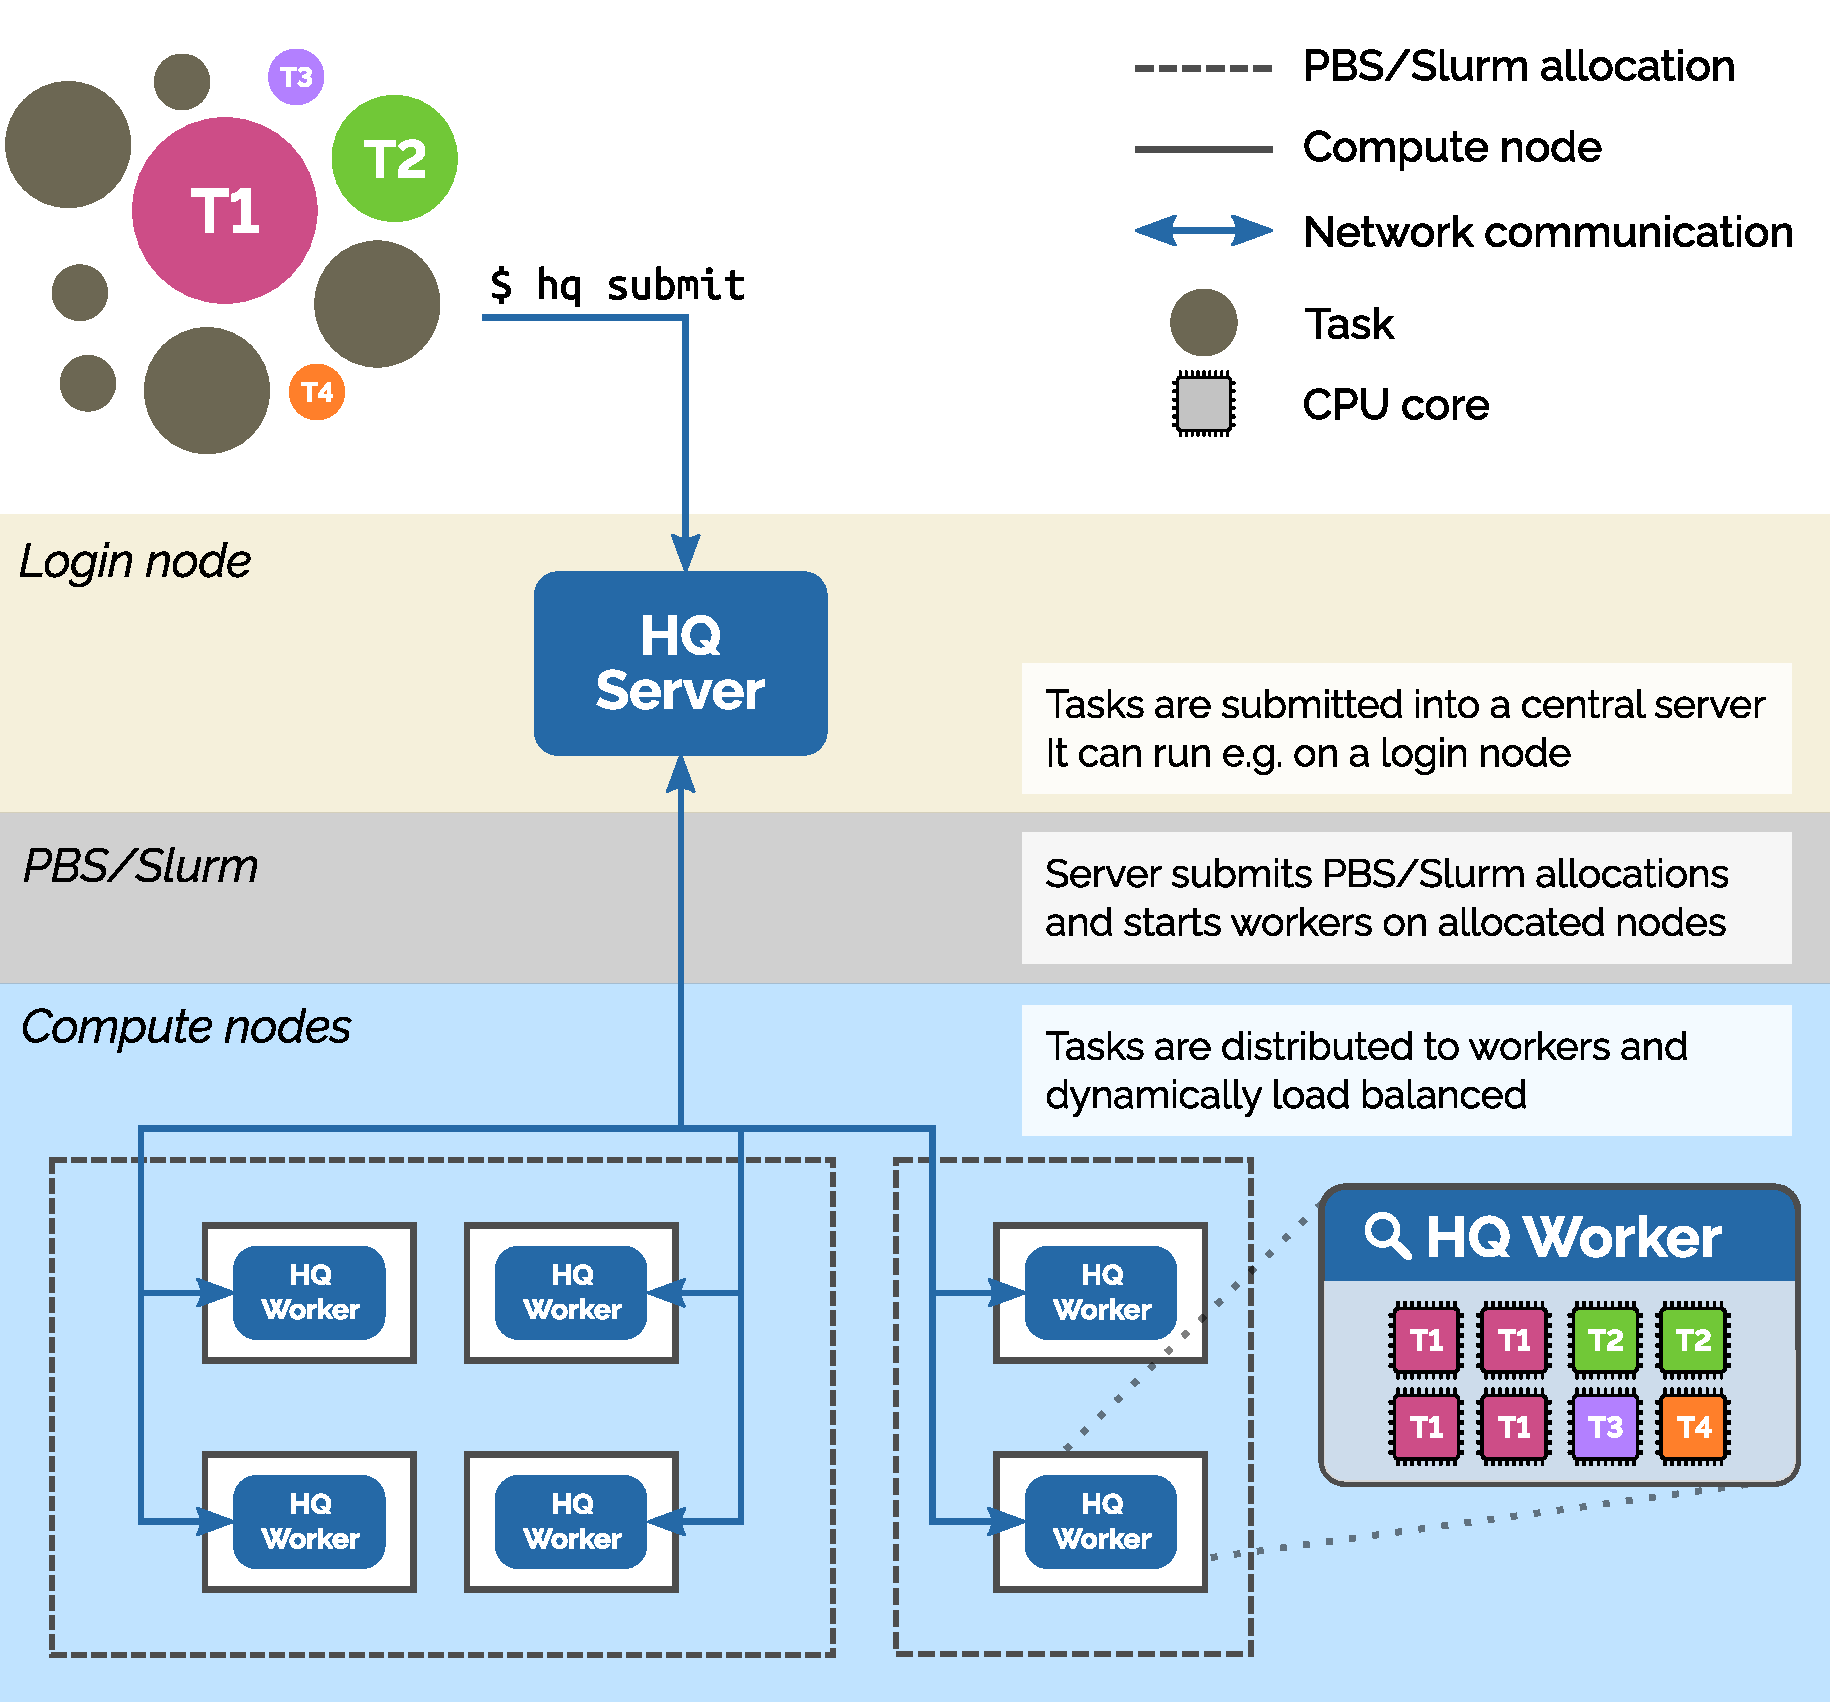
\includegraphics[width=0.7\textwidth]{imgs/hq/architecture}
	\caption{Architecture of \hyperqueue{}.}
	\label{fig:hq-architecture}
\end{figure}

\subsubsection*{Server}
The \emph{server} is the most important part of \hyperqueue{}. Its main goal is
to manage the lifecycle of both task graphs and workers; it keeps track of them and allows users to
query their state and also send commands to it through a client interface. The server contains a
work-stealing task scheduler that is based on the \rsds{} scheduler implementation
described in~\Autoref{sec:rsds-description}. The scheduler assigns individual tasks to workers based on
task resource requirements and current computational load of workers, with the goal of maximizing
hardware utilization of the connected workers.

The server is designed to be executed as a long-running background process that should ideally be
executed in a persistent location not managed by allocation managers (i.e.\ outside transient
allocations). Typically, it is executed on a login node of a cluster, but it can also run
elsewhere, for example in a cloud partition. It should keep running until all tasks that the user
wants to execute are finished, although it can also restore its state from disk, so the computation
of a task graph can be interrupted and resumed at a later time, if needed.

The fact that the server runs outside allocations allows it to load balance tasks across workers
running in multiple allocations concurrently, and work around the various limits of allocation
managers. This adheres to the first principle of the meta-scheduling design described in the
previous section.

The server itself does not execute any tasks, and it consumes a relatively modest amount of
resources; it is thus not computationally demanding.~\Autoref{sec:hq-exp-server-cpu-consumption} evaluates how many
\gls{cpu} resources the server consumes in extreme scenarios.

Apart from basic responsibilities related to task scheduling and worker management, the server also
provides additional functionality. For example, it can submit allocations fully automatically on
behalf of the user. This feature will be described in detail in~\Autoref{hq:automatic-allocation}.

The inner architecture of the server is displayed in~\Autoref{fig:hq-server-architecture}. The server is divided
into two parts; frontend and backend. The frontend part is responsible for managing a database of
task graphs and workers and providing access to it to clients. It also stores all important events
(such as a task being completed or a task graph being submitted) into a journal file, from which it
can restore its state in case of an unexpected failure. The frontend also runs the automatic
allocator, which submits allocations into Slurm or \gls{pbs} to spawn new workers.

\begin{figure}[h]
	\centering
	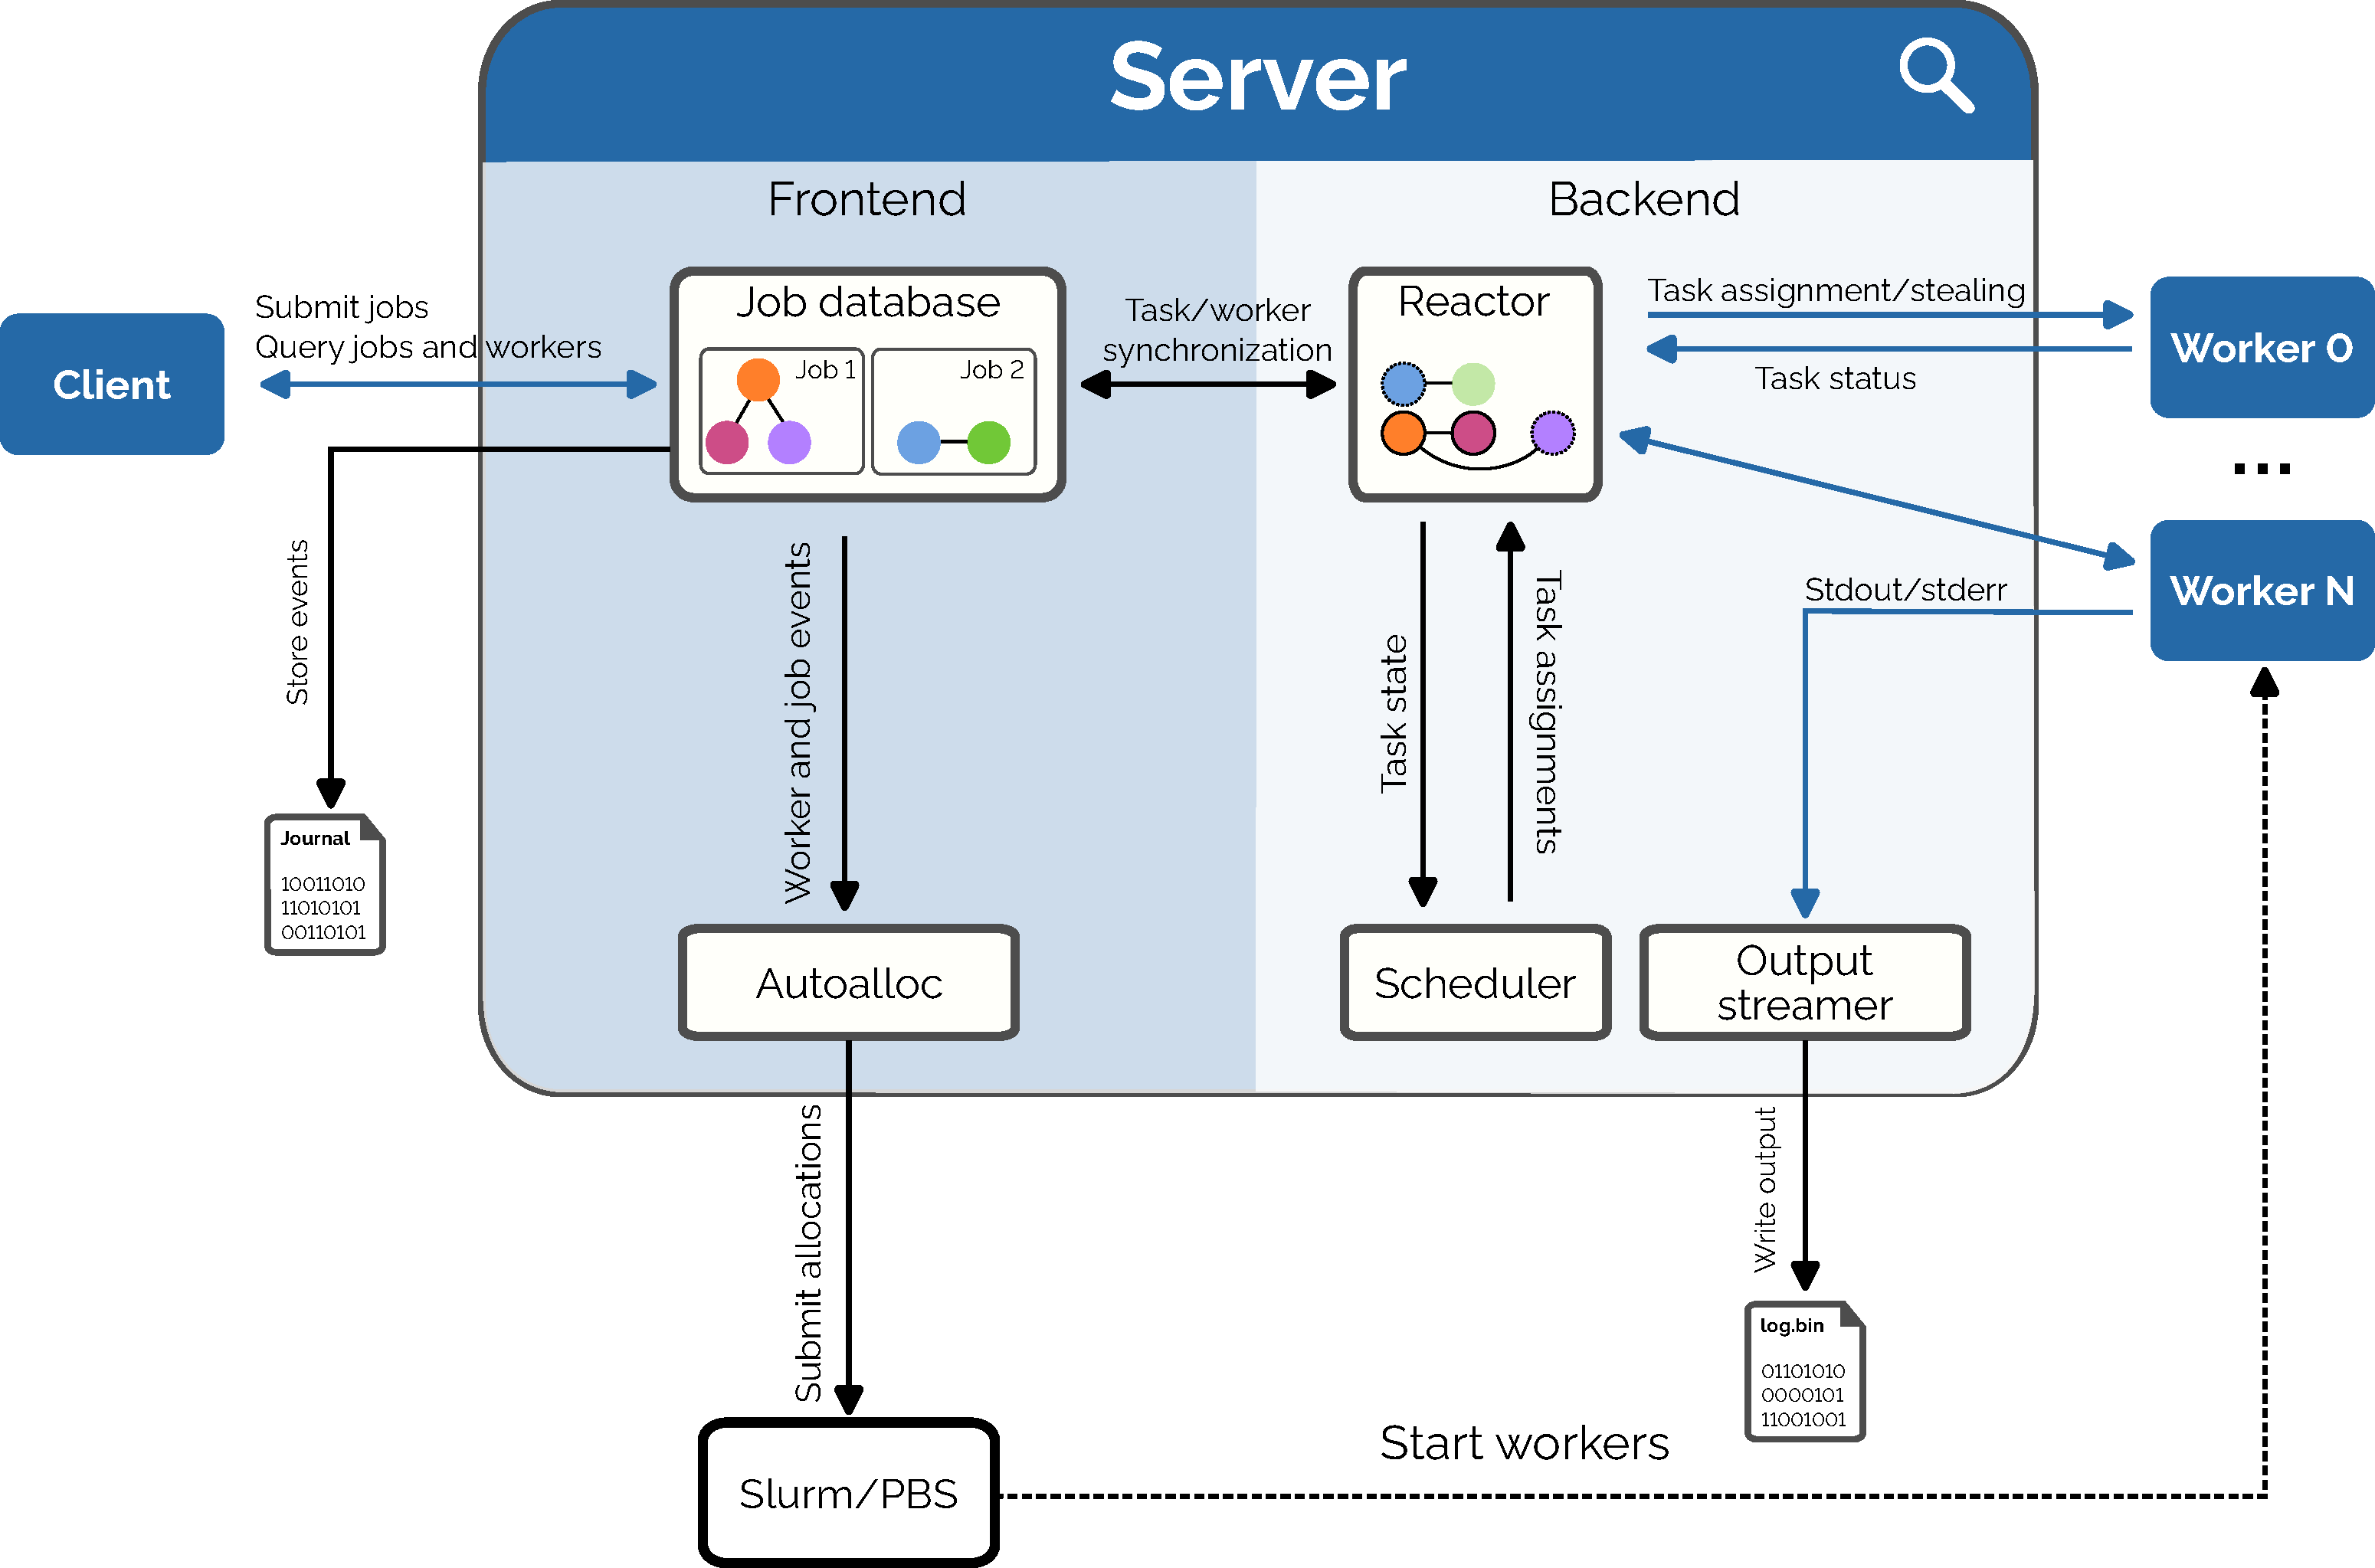
\includegraphics[width=0.9\textwidth]{imgs/hq/server-architecture}
	\caption{Architecture of the \hyperqueue{} server.}
	\label{fig:hq-server-architecture}
\end{figure}

The backend is the performance-critical part of the server. It does not separate individual task
graphs submitted by users, it simply works with a set of tasks that it schedules to workers. The
\emph{Reactor} component passes task events received from workers to a separate
\emph{Scheduler} component that computes the assignments of tasks to workers using the
\emph{b-level} heuristic and work-stealing (this implementation is based on the
\rsds{} scheduler). It then returns the schedule back to the reactor, which takes
care of sending tasks to workers that were assigned to them. The backend also contains a component
for streaming standard (error) output generated by tasks from workers into binary files, which can
be used to avoid putting too much stress on distributed filesystems. This will be described
in~\Autoref{hq:task-input-and-output}.

Even though both parts (frontend and backend) currently run inside the same Linux process, they are
strictly separated and communicate together using a well-defined interface. Therefore, it would be
possible to deploy the backend in a separate process or even run it on a different node, in which
case the two parts would communicate over the network. This could be useful for example to run the
backend on a more powerful computational node.

\subsubsection*{Worker}
The \emph{worker} component is a general computational provider that executes tasks
assigned to it by the server. A single worker typically manages all hardware resources
(\gls{cpu} cores, \gls{gpu} or \gls{fpga} accelerators,
memory, etc.) of a given computer, usually a single computational node of a supercomputer.

The worker is able to automatically detect all relevant hardware resources that are available on
the node where it is started and advertise them to the server. Therefore, in a typical case, users
can simply start the worker on a given node with a single uniform command, and from that moment on
the resources of that node will be used for task execution. This adheres to the second principle of
the proposed meta-scheduling design, where computational providers should be generic (not tied to
any specific task or a set of tasks) and it should be possible to start them using a uniform
command, to make their deployment trivial.

Each worker also participates in task and resource scheduling. The server makes high-level
scheduling decisions, such as which tasks will be executed on a given worker, while the worker then
performs micro decisions, such as in which order it will execute tasks assigned to it or which
specific resource elements will be assigned to a given task. Resource management will be described
in more detail in~\Autoref{sec:hq-resource-management}.

\hyperqueue{} workers were designed with fault tolerance in mind. On an
\gls{hpc}
cluster, workers will be typically executed inside allocations that only run for a limited amount
of time, which implies that workers can disappear at any time during the computation of a task
graph. Both the server and workers thus operate with the assumption that workers can be potentially
short-lived; if a worker disconnects while it is executing a task, the task will be transparently
reassigned to a different worker without user intervention. Worker management is thus dynamic and
flexible; new workers can also be added at any time, after which they will immediately start
contributing to the execution of the submitted task graphs. This property enables users of
arbitrarily scale the computation of a task graph both up and down even while it is being executed,
by dynamically adding or removing workers as needed.

While workers can be deployed manually by users, \hq{} can also automatically
submit allocations to an allocation manager that start workers on computational nodes based on
current computational needs of submitted task graphs, as was already mentioned. This system, called
\emph{automatic allocation}, will be described in more detail later in~\Autoref{hq:automatic-allocation}.

\subsubsection*{Client interfaces}
Users can use two main interfaces for deploying the \hyperqueue{} server and workers,
submitting task graphs and managing and monitoring the computation. They can either use a
\gls{cli}, which has been designed to feel familiar to users of Slurm in order to
make it easier to migrate existing \gls{hpc} workflows to \hyperqueue{}, or
a Python \gls{api}, which is useful for more complex use-cases that are challenging
to express using the command line. These interfaces are relatively comprehensive and their specific
shape is not crucial for this thesis; the complete set of supported \gls{cli}
commands and their parameters and the Python \gls{api} is described in the
\hyperqueue{} documentation~\cite{hq_docs}. In the rest of the text, we will
show various examples of these interfaces (primarily of various \gls{cli} commands),
to provide an idea of how ergonomic it is for users to interact with \hyperqueue{}.

The \gls{cli} has been designed with the ``Simple things should be simple. Complex
things should be possible.''\footnote{Originally coined by Alan Kay.} approach in mind. It allows submitting various
kinds of workflows in an easy way, but also allows users to configure their execution extensively.
This is in contrast to some other task runtimes, which require using Python code (e.g.\
\dask{}) or workflow files (e.g.\ \snakemake{}) for executing even the
simplest of workflows. \hyperqueue{} also supports defining task graphs using workflow
files, although it is optional and usually not needed for simple use-cases.~\Autoref{lst:hq-cli-commands}
shows three basic commands that leverage the \texttt{hq} binary to deploy an instance
of a \hyperqueue{} server and a worker, and then execute a single task through it. More
examples will be shown later throughout this chapter. For simple existing workflows defined using
Bash scripts, it is often enough to replace uses of the \texttt{sbatch} command with
\texttt{hq submit} to let \hyperqueue{} manage task execution instead of Slurm.

\begin{listing}[h]
	\begin{minted}[fontsize=\small, tabsize=4]{bash}
# Start a HQ server
$ hq server start &

# Start a HQ worker
$ hq worker start &

# Submit a HQ job (task graph) with a single task
$ hq submit ./my-program
	\end{minted}
	\caption{Examples of \hyperqueue{} \glsxtrshort{cli} commands}
	\label{lst:hq-cli-commands}
\end{listing}

\subsubsection*{Deployment}
Even though it is often overlooked, deployment of software on supercomputers can be challenging, as
was described in~\Autoref{challenge:deployment}. Since \hyperqueue{} aims to provide seamless
support for \gls{hpc} use-cases, it was also designed to be trivial to deploy. It is
distributed as a single, relatively small (approximately \SI{15}{\mebi\byte}), statically
linked executable called \texttt{hq}, which implements all the provided functionality
(server, worker and the whole \gls{cli}). It does not depend on any external services
or dynamic libraries, apart from the ubiquitous \texttt{C} standard library, and it
runs fully in userspace and does not require any elevated privileges. It also does not require any
installation nor configuration.

The \hyperqueue{} Python \gls{api} is then distributed as a Python package
that is available on the standard Python Package Index~\cite{hq_pypi}. This package
contains all the \hq{} logic inline; it is thus self-contained and does not
require the \texttt{hq} binary.

Both clients and workers communicate with the server using the standard \gls{tcpip}
protocol, which is ubiquitously available on most clusters. By default, all communication is
encrypted, so that other users of the cluster cannot read the data sent between the
\hyperqueue{} components. This is performed out of an abundance of caution, because the
server typically runs on a login node shared by multiple users, rather than on computational nodes
that are usually isolated between users by the allocation manager. The performance overhead of
encryption will be evaluated in~\Autoref{sec:hq-exp-encryption-overhead}.

In order to connect the individual components using \gls{tcpip}, normally it would be
required for users to specify network hostnames and ports. While this process is relatively simple,
it still presents a minor ergonomic hurdle, because users would need to reconfigure their worker
deployment scripts and client commands every time the server would start with a new
\gls{tcpip} address and port. To make this easier, \hyperqueue{} removes the
need to specify hostnames and ports by default, by exploiting a useful property of
\gls{hpc} clusters, which commonly use a shared networked filesystem. When a server
is created, it creates a configuration file in the user's home directory, which contains all
information necessary for exchanging handshakes and connecting the components. When workers and
clients discover the presence of this file (which can be accessed due to the filesystem being
shared), they are able to connect to the server without the user having to specify any addresses.
However, it is still possible to deploy multiple concurrent instances of \hyperqueue{}
under the same account; users just need to provide separate directories for storing the
configuration file.

Thanks to these properties, it is trivial to deploy and use \hyperqueue{} on
supercomputers even without the involvement of cluster administrators. The deployment benefits
extend beyond \gls{hpc} clusters; users can trivially deploy \hyperqueue{}
on their own personal computers. This enables them to prototype their \gls{hpc}
workflows locally, which can accelerate their development process and is another step towards
improving the ergonomics of using task graphs on supercomputers. This is in contrast with using
allocation managers for submitting tasks directly, which makes local experimentation difficult, as
allocation managers are typically not straightforward to deploy.

\subsection{Programming model}
\label{sec:hq-programming-model}
The task-based programming model used by \hyperqueue{} builds upon the task model defined
in~\Autoref{ch:taskgraphs}. It adds some additional \gls{hpc}-focused features on top
of it, such as fine-grained resource management and support for multi-node tasks.

The core element of the programming model is a \emph{task}, which has the following
properties:
\begin{itemize}[itemsep=0pt,topsep=4pt]
	\item It is a unit of computation. It can be executed by a worker (or a set of workers in the case of
	      multi-node tasks). In the current implementation, each task represents either the execution of a
	      binary executable or the invocation of a Python function.
	\item It is a unit of scheduling. The scheduler assigns tasks to workers, and can move tasks between
	      workers using work-stealing if their load is unbalanced.
	\item It forms a failure boundary. When a worker crashes while executing a set of tasks, they are
	      scheduled again onto a different worker and their execution is restarted from scratch.
	\item It is a unit of dependency management. Each task may depend on a set of other tasks; in this way
	      tasks are composed in a \gls{dag}.
	\item It is a unit of resource management. Each task has a set of resource requirements; the scheduler
	      matches them with resources provided by workers.
\end{itemize}

Each task also has various additional properties, such as a path to the executed binary (or a
Python function), a set of environment variables, a working directory, and others.

Tasks are composed into task graphs, which are called \emph{jobs} in the
\hq{} terminology. Each task belongs to exactly one job; jobs are completely
independent, so there can be no dependencies between tasks belonging to different jobs. Jobs are
units of monitoring and management, as they allow users to group many tasks together, observe their
state or perform operations on all (or a selected subset of) tasks of a job at once. There are two
kinds of jobs, \emph{graph jobs} and \emph{task arrays}. Graph jobs correspond to
arbitrary \glspl{dag}, where tasks may depend on one another. These can be only created
using the Python \gls{api} or a \gls{toml} workflow file, since it would
be difficult for users to express dependencies using a command-line interface.

Task arrays are a special case of graph jobs that use a compressed representation of a potentially
large task graph with a regular structure. For example, a common use-case is to compute a task
graph where each task runs the same computation, but on a different input. This can be achieved
with a task array, which stores only a single instance of the task definition (what should be
computed), but creates many copies of this task, each with a different input. This allows users to
easily execute large task graphs using the \gls{cli}, and it also reduces the memory
usage of the server, because the task graph is stored in a compressed format.

Each task in the task array gets assigned a different \emph{task ID}, which uniquely
identifies a specific task, which allows it to perform its computation on a different input. For
example, if a user creates a task array with a thousand tasks, then by default, the first will have
ID $1$, the second one will have ID $2$, etc. The ID is
passed to the task through an environment variable. Apart from assigning unique inputs to tasks
through task IDs, \hq{} also supports passing a unique binary blob to each task
(again through an environment variable) that can contain arbitrary data.~\Autoref{lst:hq-cli-task-arrays}
shows an example of how users may submit task arrays through the \gls{cli}.

\begin{listing}[h]
	\begin{minted}[fontsize=\small, tabsize=4]{bash}
# Task array with 10 tasks, each task gets a different ID
$ hq submit --array=1-10 ./my-script.sh

# Each task will receive a single line from the given file
$ hq submit --each-line=inputs.txt ./my-script.sh

# Each task will receive a single item from a JSON array stored in the given file
$ hq submit --from-json=items.json ./my-script.sh
	\end{minted}
	\caption{Creating task arrays using the \hyperqueue{} \glsxtrshort{cli}}
	\label{lst:hq-cli-task-arrays}
\end{listing}

\subsubsection*{Task and job lifecycle}
The server manages the state lifecycle of tasks and jobs and also reports them to the user, so that
they can observe what is happening with their computation. At any given time, each task can be in a
single \emph{state}:

\begin{description}[wide=0pt,itemsep=0pt,topsep=4pt]
	\item[Waiting] After the user creates (\emph{submits}) a task, it starts in the \emph{waiting}
		state, where it waits until all its dependencies are finished and until there is a worker that is
		able to fulfill its resource requirements.
	\item[Running] After a task is scheduled and starts executing on a worker, it moves to the \emph{running}
		state. If the worker that is executing the task stops or crashes, the task will move back to the
		\emph{waiting} state, so that it can be rescheduled to a different worker. This is labeled
		as a \emph{task restart}.
	\item[Finished] When a task finishes successfully (a binary program exits with the exit code $0$
		or a Python function returns without throwing an exception), it moves to the \emph{finished}
		state.
	\item[Failed] When a task fails (a binary program exits with a non-zero exit code or a Python function throws an
		exception), it moves to the \emph{failed} state.
	\item[Canceled] When a waiting or a running task is canceled by the user, it moves to the \emph{canceled}
		state, and it is no longer considered for execution. Users can cancel tasks and jobs that are no
		longer relevant and that should not continue executing.
\end{description}

\Autoref{fig:hq-task-state-diagram} displays a state diagram of the various task states and
transitions that cause state changes. The \emph{finished}, \emph{failed} and
\emph{canceled} states are terminal; once a task reaches that state, it cannot change its
state anymore. Each job also has its associated state that is derived from the state of its tasks.

\begin{figure}[h]
	\centering
	\begin{tikzpicture}
		\tikzstyle{every node}=[font=\footnotesize]
		\tikzstyle{every state}=[fill={rgb:black,1;white,8},minimum size=1.5cm,font=\footnotesize]

		\node[state,initial,initial text=Submitted]   	(waiting)  							{Waiting};
		\node[state] 							   		(running) 	[right=2.5 of waiting]	{Running};
		\node[state,accepting]           		   		(finished) 	[right=2 of running]	{Finished};
		\node[state,accepting]                     		(failed) 	[above=1 of finished] 	{Failed};
		\node[state,accepting]                     		(canceled)	[below=1 of finished]   {Canceled};

		\path[->]
		(waiting)   edge [bend left]	node [above] 			{Scheduled} 		(running)
		(waiting)   edge [bend right]	node [below left]		{Canceled}			(canceled)
		(running)	edge    			node [above] 			{Finished}			(finished)
		(running) 	edge    			node [above left] 		{Failed} 			(failed)
		(running)	edge    			node [left,xshift=-5]	{Canceled} 			(canceled)
		(running)	edge [bend left]    node [below,xshift=8]	{Worker crashed}	(waiting);
	\end{tikzpicture}
	\caption{State diagram of \hyperqueue{} tasks}
	\label{fig:hq-task-state-diagram}
\end{figure}

\subsubsection*{Iterative computation}
Iterative computation, such as running a simulation until it converges or training a
machine-learning model, can be expressed using the concept of \emph{open jobs}. Such jobs
allow users to dynamically add tasks to them, even if some tasks were already computed. This can be
used to perform several iterations until some condition is met within the same job, without
unnecessarily creating a new task graph (job) for each iteration. This makes it easier to express
arbitrarily dynamic task graph structures where the shape of the graph is not fully known before
the computation starts.

\subsection{Task input and output}
\label{hq:task-input-and-output}
By default, each \hyperqueue{} task stores its \emph{standard output} (\emph{stdout}) and
\emph{standard error output} (\emph{stderr}) streams to the filesystem. Users can override this to avoid storing these
output streams, or to let \hq{} remove them if they are empty after the task has
finished executing, to reduce disk clutter. It is also possible to use various placeholders for
configuring the paths of these streams. For example, the string \texttt{\%\{TASK\_ID\}} in a stream
path will get resolved to the task ID of the task that produces the stream. This can be used to
easily separate the output of different tasks.

Since task graphs can be large, generating two files per task, especially on shared network
filesystems that are commonly used on supercomputers, could cause performance bottlenecks or run
into limitations caused by user disk quotas. To alleviate this problem, \hq{}
supports an output management system called \emph{output streaming}. If it is enabled for a given
job, then \emph{stdout} and \emph{stderr} of tasks is streamed over the network
from workers to the server, instead of being stored into separate files. The server then stores all
this data into a single \emph{logfile}. It also offers several commands for manipulating
and filtering task output data from this file. This helps to reduce the pressure put on the
filesystem.~\Autoref{sec:hq-exp-output-streaming} will evaluate how this system can help resolve potential
\gls{io} issues.

%~\Autoref{lst:hq-cli-log} shows several \hq{}
%commands that can be used to interact with output streaming.

%\begin{listing}[h]
%	\begin{minted}[fontsize=\small, tabsize=4]{bash}
%# Submit a job with output streaming enabled
%$ hq submit --log=log.bin --wait -- ./my-program
%
%# Print stdout of tasks 1 to 10 from the log
%$ hq log log.bin cat --task 1-10 stdout
%
%# Export the log into a JSON format
%$ hq log log.bin export
%	\end{minted}
%	\caption{\hyperqueue{} \glsxtrshort{cli} commands for working with output streaming}
%	\label{lst:hq-cli-log}
%\end{listing}

\hyperqueue{} currently does not support data transfers between tasks. Arbitrary binary
data can be attached as an input for any task (through its \emph{standard input} stream), but
task outputs are only used for specifying dependencies; they cannot be transferred between the
workers directly. This is only relevant for the Python \gls{api}, because tasks
submitted using the \gls{cli} cannot easily express data transfers. The
\hq{} server is based on the \rsds{} server implementation, which
supports data transfers between workers, so the transfer functionality itself is actually
implemented in \hq{}. However, data transfers still need to be incorporated into
the \hyperqueue{} programming model, and a user-facing (Python) interface for consuming
outputs of tasks needs to be designed. It should be noted that this is a limitation of the current
implementation that we plan to lift in future work.

\subsection{Resource management and scheduling}
\label{sec:hq-resource-management}
As has already been mentioned, the \hyperqueue{} scheduler is derived from the
\rsds{} work-stealing scheduler that was described in~\Autoref{sec:rsds-description}. It
assigns tasks to workers eagerly, to optimize the fast path where there are enough tasks to utilize
the available workers. When some workers are underutilized, the server uses work-stealing to steal
tasks between workers to balance the computational load. Scheduling is performed on the level of
tasks, regardless of which job they belong to; the scheduler does not even know anything about
jobs, as they exist only in the frontend.

What makes the scheduler different from \rsds{} is its support for the complex
resource management scenarios that were described in~\Autoref{sec:heterogeneous-resources}. It supports
non-fungible resources, related resources, fractional resource requirements, resource variants and
also multi-node tasks in a single unified resource system. When a task is being scheduled, the
scheduler looks for a worker that can satisfy all resource requirements of that task, based on the
amount of resource elements that the worker currently has available. When a task is scheduled onto
a worker, the scheduler \emph{allocates} a specific subset of the worker's resources to that
task, which will not be available for other tasks until that task finishes its execution.

\hyperqueue{} resources are \emph{generic}; users can define their own
arbitrary resource kinds for both tasks and workers. At the same time, \hq{} also
recognizes several known resource names and provides specialized support for them. Resource
management in \hyperqueue{} consists of two main systems, resource pools provided by
workers and resource requirements specified by tasks. They will be described in turn below.

\subsubsection*{Worker resource pools}
Worker resources are configured when a worker is started through so-called \emph{resource pools},
named sets of resource elements. The most common resource pools, such as \gls{cpu}
cores and their \gls{numa} sockets, the amount of \gls{ram} and the
presence of \gls{gpu} accelerators are detected automatically. On top of that, users
can specify an arbitrary set of additional pools. There are two kinds of resource pools:

\begin{description}[wide=0pt]
	\item [Indexed pool] represents a set of resource elements where each individual element is
	      non-fungible and has a unique identity (represented either by an integer or a string). An example
	      of such a resource pool could be a set of \gls{cpu} cores or \gls{gpu}
	      devices. For example, if a worker has two NVIDIA \glspl{gpu}, that worker could provide
	      an indexed pool containing two elements (e.g.\ with indices $0$ and
	      $1$), each representing one individual \gls{gpu} device. These two
	      resources are not interchangeable; the scheduler decides which specific element will be assigned to
	      a task and it tracks the individual elements based on their identity. If a task
	      $t$ is currently using \gls{gpu} $0$, that
	      element will not be assigned to any other task until $t$ has finished being
	      executed.

	      Individual elements of an indexed pool can be further subdivided into \emph{groups}, which
	      mark some form of a relationship between specific elements. This can be used to represent
	      \emph{related resources}, e.g.\ \gls{numa} domains and \gls{cpu} sockets; a
	      worker might provide a single indexed pool of \glspl{cpu} with a separate group for each
	      \gls{numa} socket present on its node. Tasks can then specify if they want to
	      prioritize drawing resources that belong to the same group; this will be described later.

	      When a worker is started, by default it automatically divides \gls{cpu} cores into
	      groups according to their \gls{numa} nodes. However, the concept of groups is general;
	      they can be used for any indexed pool, not only specifically for \gls{numa}.
	\item [Sum pool] is designed for resources that are fungible. Such resources are typically
	      numerous and it would thus be impractical to track each individual resource element separately. A
	      sum pool does not represent its individual elements with indices; it simply defines a single number
	      that specifies the amount of resources available in the pool. A typical representative of a sum
	      pool is the amount of \gls{ram} available on a worker node. Modern
	      \gls{hpc} nodes can contain hundreds of GiBs of memory; it would be infeasible to
	      treat each byte as a separate resource element. At the same time, tasks usually do not need such
	      fine-grained tracking for these kinds of resources; if they care about memory requirements, they
	      can just specify how much memory they need.
\end{description}

\Autoref{lst:hq-cli-worker-resources} shows a few examples of how users can configure resources
when starting workers through the \gls{cli}.

\begin{listing}[h]
	\begin{minted}[fontsize=\small, tabsize=4]{bash}
# Start a worker with automatically detected resources
$ hq worker start

# Start a worker that manages 16 CPU cores
$ hq worker start --cpus 16

# Start a worker with additional resources
# Adds an indexed pool of four GPUs and a sum pool of 1024 resources (bytes)
$ hq worker start \
	--resource 'gpus/nvidia=[0,1,2,3]' \
	--resource 'memory=sum(1024)'
	\end{minted}
	\caption{Configuring worker resources using the \hyperqueue{} \glsxtrshort{cli}}
	\label{lst:hq-cli-worker-resources}
\end{listing}

\subsubsection*{Task resource requirements}
Resource pools define the resources that are available on workers. The scheduler then uses
\emph{resource requirements} attached to individual tasks to decide on which workers a given task can be
executed and which specific resources it will consume while it is running. Task resource
requirements are defined for each task separately. By default, each task requires a single
\gls{cpu} core, but users can specify a different \gls{cpu} requirement
and also add additional requirements.

A resource requirement consists of a name of the resource that the task needs (the resource kind)
and an amount specifying how many such resources are needed. For example, a task might specify that
it requires two \glspl{gpu} for its execution. The resource requirement always
specifies the amount of required resources, regardless of whether the given resource is drawn from
an indexed pool or a sum pool.

Task resource requirements in \hyperqueue{} also support related resources, fractional
resources, and dynamic resource selection (resource variants). These allow tasks to describe more
complex use-cases related to resource management. The implementation specifics of these resource
management features are described below.

\vspace{2mm}\textbf{Fractional resource requirements}\enskip{}Tasks can specify
their resource requirements in the form of a fraction. The scheduler uses fixed-point arithmetic to
manage fractional resource requirements, in order to avoid issues associated with floating-point
arithmetic, such as rounding errors.

\vspace{2mm}\textbf{Resource variants}\enskip{}Each task can define a list of
resource requirement sets (resource variants); the scheduler uses the first one that can be
satisfied by a worker at the time of scheduling. The order of the variants in the list determines
their priority. The load-balancing improvements that can be achieved using resource variants will
be evaluated in~\Autoref{sec:hq-exp-resource-variants}.

\vspace{2mm}\textbf{Related resources}\enskip{}Relations between resource
elements can be modeled using a combination of indexed pool groups and a \emph{group allocation strategy},
which can be used to choose which specific resource elements from an indexed pool will be used for
a given task. A typical example where indexed pool groups are useful are \gls{numa}
nodes, where tasks might want to be executed on cores that belong to the same
\gls{numa} node (group). Tasks can use one of the following three strategies for each resource kind
that they request:

\begin{description}[wide=0pt,itemsep=0pt,topsep=1pt]
	\item [Compact] is the default strategy. The scheduler tries to allocate all requested
	      resources from as few groups as possible. However, if there are not enough resources currently
	      available for that approach on a given worker, it will also try to draw resource elements from a
	      larger number of groups in order to satisfy the resource requirement.
	\item [Strict compact] is a stricter version of the \emph{compact} strategy. With this
	      strategy, the scheduler first figures out the minimum number of groups required to satisfy the
	      resource requirement. It will then schedule the task only after it can provide all requested
	      resources from the smallest number of groups possible.
	\item [Scatter] is the opposite of the \emph{compact} mode. It tries to allocate resources
	      for the task from as many groups as possible.
\end{description}

The effect of group allocation strategies will be evaluated in~\Autoref{sec:hq-exp-numa}. Note that
these strategies are not relevant for sum pools nor for indexed pools with a single group.

Furthermore, resource requirements can also be specified without an upper bound, i.e.\ a task can
specify that it wants to consume all available resources of the specified pool. If a worker has at
least a single resource element of the given pool available and the scheduler assigns a task with
this kind of resource requirement to it, that task will be allocated all the pool's resources that
are available when the task starts to execute. This can be used for software that is scalable
w.r.t.\ the amount of resources provided to it.

There is also one additional special resource that is relevant for scheduling, called a
\emph{time request}. If a task specifies a time request (a duration) $t$, it
tells the scheduler that it needs at least $t$ time units for its execution.
This is important for avoiding needless task restarts. Because workers started in allocations
cannot run for a longer time than their allocation's wall-time (which is a known value), the
scheduler knows the remaining lifetime of each such worker at any given time. This information is
used for scheduling; if a worker has remaining lifetime $l$, the scheduler will
not assign it tasks with a time request that is longer than $l$, because it is
probable that such tasks could not finish executing before that worker shuts down.

Once a task is scheduled to a worker and the scheduler decides which resources will be allocated to
it, it passes this information to the task through environment variables. For example, if a task
asks for two \gls{cpu} cores and the scheduler allocates cores $10$
and $14$ of a specific worker to it, \hq{} will pass the
environment variable \texttt{HQ\_RESOURCE\_VALUES\_cpus=10,14} to the task.

It is important to note that \hyperqueue{} treats resources as opaque and virtual; they
are used only for scheduling. For example, if a task is provided with cores $0$
and $1$, the worker that executes it does not enforce that it will actually run
on these specific cores. This responsibility is left to the task itself, which can use the provided
environment variable to decide which resources it should actually use for its execution. For
example, a task could pin its threads onto cores that were allocated to it. In the case of
\gls{cpu} cores, \hq{} can pin the allocated cores for the task
automatically if the task is configured as such.

\Autoref{lst:hq-cli-task-resources} displays a few examples of how can task resource requirements be
configured using the \gls{cli}.

\begin{listing}[h]
	\begin{minted}[fontsize=\small, tabsize=4]{bash}
# Submit a task requiring 4 CPU cores
$ hq submit --cpus=4 ./my-program

# Submit 1000 tasks, each requiring 2 CPU cores
$ hq submit --cpus=2 --array=1-1000 ./my-program

# Submit a task requiring 2 CPU cores, pin CPU cores using OpenMP
$ hq submit --cpus=2 --pin=omp ./my-program

# Submit a task that requires 2 FPGA devices and needs at least 10 minutes to execute
$ hq submit --resource 'fpga=2' --time-request 10m ./my-program
	\end{minted}
	\caption{Configuring task resource requirements using the \hyperqueue{} \glsxtrshort{cli}}
	\label{lst:hq-cli-task-resources}
\end{listing}

\subsubsection*{Multi-node tasks}
\hyperqueue{} also supports a special kind of a resource that is especially useful for
tasks that want to execute \gls{hpc} applications designed to run on multiple nodes
(e.g. \gls{mpi} programs). A task may specify that it wants to be executed on
multiple workers at the same time. In this case, \hq{} assumes exclusive
ownership of all the resources of each worker (node), which typically matches the requirement of
\gls{mpi}-like applications. A multi-node task requiring $n$ nodes
can only be scheduled when $n$ workers are idle (not executing any tasks) at the
same time. When a multi-node task starts to execute, \hq{} passes it a
\emph{nodefile} which contains the hostnames of all workers allocated to the task. This
nodefile can then be used by common \gls{mpi} program launchers to start an
\gls{mpi} program.

Users that execute multi-node tasks running \gls{mpi} applications might want to make
sure that all workers (nodes) contributing in this computation are started in the same allocation,
primarily for performance reasons (e.g.\ they might configure allocations to use nodes that reside
close together in the networking topology of the cluster). By default, \hyperqueue{}
tries to adhere to this constraint. It uses an abstract concept of \emph{worker groups};
multi-node tasks are always scheduled to workers belonging to the same group. At the same time, the
group of a worker is automatically configured based its allocation (if there is any). This ensures
that multi-node tasks are by default executed only on workers that reside within the same
allocation. However, it is possible to override the group of a worker and e.g.\ assign the same
group to all workers. In that case, workers from all active allocations can participate in
executing multi-node tasks.

\subsection{Fault tolerance}
The execution of a task in \hyperqueue{} can end in a failure because of two main
reasons. The worker that executes the task might crash, be stopped by the user, or an allocation
inside which it is executed can run out of its wall-time. In that case, the task will be
rescheduled by the server to a different worker that upholds its resource requirements. This is
made possible due to the fact that tasks are not tied to any specific computational resource or
allocation. When such a task restart happens, it is important to let the executed program know that
it is not being executed for the first time, so that it can react to it (for example clean up files
that were created during a previous execution of the same task or restore execution from a
previously created checkpoint). This is achieved using an \emph{instance ID}. It is a
non-negative number attached to each task that is increased every time the task is restarted. This
number is then passed to the executed task so that it can decide whether it should react to the
restart in any specific way.

In rare cases, the crash of the worker might be caused by the task itself, e.g.\ if it allocates
too much memory and causes an \gls{oom} failure. If this happens repeatedly, such
task could hamper the execution of the whole task graph, since it would be repeatedly crashing
workers. For that reason, it is possible to configure the maximum number of worker crashes per task
(it is configured to a low number by default). If a task exceeds this number (i.e.\ it is present
during too many worker crashes), it will be automatically canceled.

The second reason why a task might fail is that its computation simply does not succeed, for
example due to the executed process returning a non-zero exit code. In that case, the task is
marked as failed and any tasks that (transitively) depend on it are canceled.
\hyperqueue{} allows users to filter tasks by their state and resubmit only failed or
canceled tasks in a straightforward way, which is possible due to the job state being kept outside
of transient allocations.~\Autoref{lst:hq-cli-fault-tolerance} demonstrates how users can use the
\hq{} \gls{cli} to resubmit failed tasks from a previously
submitted job. It also shows that several \hq{} commands are designed to be
composable, adhering to the Unix philosophy of creating commands that do a single thing well and
that can be easily combined together.

\begin{listing}[h]
	\begin{minted}[fontsize=\small, tabsize=4]{bash}
# Submit task array with 1000 tasks, wait until it completes
$ hq submit --array=1-1000 --wait ./my-script.sh

# Find task IDs that have failed in the last job
$ FAILED_TASKS=$(hq job task-ids last --filter=failed)

# Resubmit only the failed tasks
$ hq submit --array=${FAILED_TASKS} ./my-computation
	\end{minted}
	\caption{Handling task failure using the \hyperqueue{} \glsxtrshort{cli}}
	\label{lst:hq-cli-fault-tolerance}
\end{listing}

Too many tasks failing can signal the presence of some catastrophic condition, e.g.\ the user
failed to properly configure their program, forgot to load some required runtime dependencies or
used the wrong filesystem path for inputs. If this happens for a very large job, it could lead to a
lot of wasted computation, where tasks will start to execute, but they will probably fail very soon
after that. \hyperqueue{} thus allows users to configure a parameter that specifies the
maximum number of task failures per job. If the configured number of failures is exceeded,
\hq{} will preemptively cancel the whole job to avoid wasting computation.

A special case of a failure is when the server itself crashes or it is stopped by the user or when
a worker loses connection to the server due to networking issues. In this case, the worker cannot
reasonably continue executing long-term without having a communication channel with the server.
However, if it manages tasks that are already being executed, it could be wasteful to stop their
computation just because the connection to the server has been lost. The worker can thus be
configured in a way that it will finish executing such running tasks before shutting itself down.
However, the completion of these tasks will not be reported back to the server (as the worker
cannot reach it anymore), so users will need to process their outputs manually.

It is possible to configure the server to store a journal containing all necessary information
about its task database to the filesystem. The server can then be restored from this journal in
case of a crash or a failure, so that it can resume computation of previously unfinished tasks.

\subsection{Automatic submission of allocations}
\label{hq:automatic-allocation}
The meta-scheduling design employed by \hyperqueue{} resolves most of the challenges
associated with using allocation managers for executing tasks, since it fully automates the mapping
of tasks to allocations. It also makes creating allocations simple, so that users can scale the
computational resources used for computing their task graphs at their will. However, creating
allocations manually can still be relatively demanding for users, who might want to employ a more
automated approach for scaling computational resources. Since \hyperqueue{} knows the
state of all tasks and workers and it is commonly executed on login nodes that have access to
allocation managers, it is natural to provide it with the ability to automatically submit new
allocations on behalf of the user, based on current computational load. This system has been
implemented in \hq{} under the name \emph{Automatic allocator} (shortened as \autoalloc{}). The automatic
allocator was created with the following design goals:

\begin{description}[wide=0pt,itemsep=0pt,topsep=2pt]
	\item[Allow computational resources to scale up] At any given moment, if there are tasks that are waiting to be executed and there are no free
		computational resources, \autoalloc{} should attempt to add more resources by creating
		new allocations. At the same time, it should respect backpressure from the allocation manager to
		avoid overloading it.
	\item[Allow computational resources to scale down] Keeping allocations running on a supercomputer can be quite costly. \Autoalloc{} should
		thus shut down allocations that are not performing any useful work (because they do not have
		anything to compute) in order to avoid wasting resources.
	\item[Be flexible] Allocation managers typically provide various configuration knobs that can affect the behavior of
		allocations. While it will not ever be possible to support all possible implementations of
		allocation managers out-of-the-box, \autoalloc{} should provide extension points that
		would enable users to configure the submitted allocations to their liking.
\end{description}

\Autoalloc{} has been implemented as a background service within the
\hyperqueue{} server. To use it, users first need to create at least one
\emph{allocation queue}. Such a queue describes a template for creating new allocations that will
be submitted by \hq{} when there is a demand for more computational resources.
Each queue contains several properties that can be configured by users:

\begin{description}[wide=0pt,itemsep=0pt,topsep=2pt]
	\item[Allocation manager] \Autoalloc{} needs to communicate with a given allocation manager
		to be able to submit allocations into it. Users thus need to tell \hq{} which
		allocation manager it should communicate with. Currently, two managers are supported, Slurm and
		\gls{pbs}.
	\item[Time limit] This value determines the wall-time of each allocation submitted by \autoalloc{}.
		Knowing the maximum duration of each allocation helps it decide when it makes sense to create
		allocations. For example, if the only tasks waiting to be computed have a \emph{time request}
		that is longer than the time limit of a given allocation queue, it does not make sense to create
		allocations in this queue, because workers started in these allocations could not execute such
		tasks anyway.
	\item[Backlog] This parameter specifies the maximum number of allocations that can be queued in the allocation
		manager at any given time. It is designed to ensure that the automatic allocator does not overload
		the allocation manager.
	\item[Worker count per allocation] Determines how many nodes (workers) should be requested for each allocation. Unless users want to
		execute multi-node tasks, it is usually convenient to use the default value
		($1$); typically, the fewer nodes are requested in an allocation, the sooner it
		will be started by the allocation manager.
	\item[Max worker count] This parameter can be used to limit the maximum number of running workers across all allocations
		started by this queue.
	\item[Idle timeout] Time after which an idle worker (a worker that does not have any tasks to compute) will stop. The
		idle timeout mechanism helps to avoid resource waste by stopping workers that do not have anything
		to compute anymore. By default, this timeout is set to a few minutes.
	\item[Worker resources] Users can override the resources assigned to each worker started by the given allocation queue.
		This can be used if the user knows that the allocations will be started in a specific partition of
		the cluster that contains resources that cannot be automatically detected by
		\hyperqueue{} (e.g. \gls{fpga} devices).
	\item[Custom allocation parameters] Users can also specify arbitrary command-line parameters that will be passed to the submit command
		sent to the corresponding allocation manager, like the computational project that should be used or
		the cluster partition where the allocation should be created. To make debugging easier,
		\hyperqueue{} will by default submit a test allocation immediately after the allocation
		queue is created, in order to test that the specified allocation parameters can be handled by the
		manager. If this test allocation is successfully created, it is then immediately canceled to avoid
		wasting computational resources.
\end{description}

\Autoref{lst:hq-cli-autoalloc} shows several examples of commands for creating allocation queues and
observing allocation state using the \hyperqueue{} \gls{cli}.

\begin{listing}[h]
	\begin{minted}[fontsize=\small, tabsize=4]{bash}
# Create an allocation queue for Slurm
$ hq alloc add slurm --time-limit 1h -- -Aproject-1 -pcpu_partition

# Create an allocation queue for PBS with GPU resources
$ hq alloc add pbs --resource "gpus/nvidia=range(0-1)" ...

# Display information about allocations submitted by the given queue
$ hq alloc info 1
	\end{minted}
	\caption{Handling task failure using the \hyperqueue{} \glsxtrshort{cli}}
	\label{lst:hq-cli-autoalloc}
\end{listing}

\Autoalloc{} is a reactive system. It observes events from the server (such as new jobs
being submitted or new workers being connected) and manages allocations in response to these
events. If it encounters a situation where there are tasks that are in the waiting state and no
existing workers can execute them (either because there are no workers or all of them are fully
occupied), it will start submitting allocations to the allocation manager. It will submit
allocations up until the configured \emph{backlog} value or until the allocation manager
applies backpressure (whichever comes sooner). Note that \autoalloc{} does not limit the
total number of allocations that are ``in-flight'' (queued or running) by default, only the number
of queued allocations. This allows it to potentially create a large number of allocations and thus
make use of all available resources of the cluster if the allocation manager allows it. Users can
use other configuration parameters (such as the total number of workers) to limit the amount of
submitted resources. \Autoalloc{} also contains an internal rate limiter that makes sure
that it does not submit allocations too quickly and that it pauses the allocation process if the
allocations start failing too often.

\hyperqueue{} communicates with \gls{pbs} or Slurm using their standard
commands, such as \texttt{qsub} or \texttt{sbatch}, as they do not provide a
completely machine-readable \gls{api}. This means that in order to use automatic
allocation, the server has to be executed on a node that has access to these commands and can
communicate with the manager. If this is not possible, a proxy service could be used to forward
communication between the node with the server and a node where the manager is deployed.
\hyperqueue{} implements communication with each manager in a custom way. While there
have been some attempts to create a unified interface~\cite{psij,workflow-alloc-manager-comm} for submitting
allocations to different allocation managers, they have not seen wide adoption so far. Furthermore,
adopting these approaches would require \hq{} to introduce a dependency on Python
or an external \gls{http} service, which would make it more difficult to deploy.

It is crucial for \autoalloc{} to maintain an up-to-date state of its created
allocations, so that it can report their state to the user and also so that it knows if it should
submit new allocations. Originally, it was using a polling approach to determine the latest state,
where it was repeatedly querying the allocation manager about the state of allocations. However,
this turned out to put a lot of pressure on the allocation managers, which were not very optimized
for this use-case, especially if the polling frequency was very high (every few seconds). Some
allocation managers are even configured in a way where they cache the state of allocations when
they are queried too often; this reduces the chance of them being overloaded, but it also means
that \hyperqueue{} would not get the latest data, which is not ideal. However, we can
observe that it is not actually required to poll the allocation manager. The only allocation events
that are important for the allocator are the start and an end of an allocation. And this
information can be learned through a proxy; the connections are disconnections of
\hq{} workers. When a worker is started in an allocation, it will connect to the
server and tell it its allocation ID\@. This lets the automatic allocator learn about new
allocations. On the other hand, when such a worker disconnects, it signifies that its containing
allocation has also finished. Using this approach, the allocator is able to maintain the latest
state of allocations without explicitly querying the allocation manager.

\Autoalloc{} attempts to take certain task properties into account when creating
allocations. For example, if a task has a \emph{time request} of two hours, but a configured
allocation queue only has a time limit of one hour, the allocator will not submit allocations using
this queue to provide resources for such a task, because workers started in these allocations could
not compute such a task anyway. It should be noted that in general, it is very difficult to guess
when and how many allocations should be created, because the allocator does not know in advance
which tasks will be submitted in the future, nor for how long the currently submitted tasks will
run. It also cannot precisely predict how long its submitted allocations will stay in the
allocation manager queue. As a future extension, the allocator could be extended with a prediction
of allocation queuing times~\cite{allocation-duration-prediction} or with a prediction of task execution
times~\cite{task-duration-prediction}.

%\Autoref{sec:hq-exp-autoalloc} will evaluate how well the automatic allocation system is able to
%scale in response to computational demand and how it limits the waste of computational resources.

\section{Use-cases}
This section describes several use-cases where \hyperqueue{} has been successfully used
to execute task graphs on \gls{hpc} systems. Apart from these selected case studies,
it has also been used in other projects and scenarios; these will be enumerated
in~\Autoref{ch:conclusion}.

The firs two use-cases originate from the LIGATE (LIgand Generator and portable drug discovery
platform AT Exascale)~\cite{ligate} project, whose goal was to integrate state-of-the-art
\gls{cadd} tools into a unified platform designed for executing drug design
experiments on petascale and exascale \gls{hpc} clusters. This project provided
funding for the development of \hyperqueue{}, and its use-cases also served as one of the
main driving forces behind the design of this task runtime. The usage of \hyperqueue{}
within the LIGATE project is also briefly described in~\cite{ligate}.

\subsection{Virtual screening and free-energy calculations}
\label{sec:hq-usecase-ligen}
One of the \gls{md} frameworks that were used in the LIGATE project was
LiGen~\cite{ligen,ligen_exscalate}, a suite of utilities that can be used for performing virtual
screening. Virtual screening is a computational method for identifying molecules that can bind to
drug candidates, which is used for computer-driven drug discovery.

LiGen was used to implement a high-throughput virtual screening pipeline, whose goal was to assign
scores to a large number of input ligands and then perform molecular docking for the most promising
ligand candidates. The primary input for the workflow is a set of ligands in the
SMILES~\cite{smiles} format, where each line represents a single ligand. LiGen then
expands each ligand into a 3D representation stored in a Mol2~\cite{mol2} format and
performs virtual screening to assign a score to it. The resulting ligand-score pairs are then
stored in a \gls{csv} file. Finally, the most promising $N$
candidates (where $N$ is a configurable parameter) are selected based on their
scores and molecular docking is then performed on them.

The virtual screening workflow has been implemented using \hyperqueue{}, in order to
leverage its heterogeneous resource management capabilities. It was designed using the Python
\gls{api}, due to its support for task dependencies and also because it was natural
to implement several utility tasks within the workflow in Python rather than e.g.\ in Bash. The
workflow consists of both very short running tasks (such as ligand expansion) and also more
computationally demanding tasks (such as scoring and docking). The scoring and docking stages can
also run on \gls{gpu} accelerators, which provide much higher throughput than the
\gls{cpu} implementation. These constraints were encoded using
\hq{} resource requirements, which allowed selecting the proper hardware
resources for each kind of task. \Autoref{sec:hq-exp-ligen} describes an experiment that measures the
achieved hardware utilization when running this workflow with \hyperqueue{}.

This workflow was executed on four computational sites; the Karolina~\cite{karolina},
LUMI~\cite{lumi}, LEONARDO~\cite{leonardo} and E4~\cite{e4}
\gls{hpc} clusters. The only change required to port the workflow to a new cluster
was to update the Slurm credentials used for submitting allocations. This demonstrates the
simplicity of porting \hyperqueue{} workflows between different supercomputers.

The output of the scoring and docking stages of the virtual screening workflow then serve as input
for a more complex \gls{cadd} workflow that is designed for performing free-energy
calculations that estimate the \gls{rbfe} of ligands and protein-hybrid ligand
complexes using \gls{awh} calculations~\cite{awh}. The
\gls{cadd} workflow uses the GROMACS \gls{md}
framework~\cite{gromacs} along with tens of other bioinformatics tools and packages and is
structurally quite complex, as it consists of tens of different Bash and Python scripts that depend
on the outputs of one another. This workflow has been also implemented using the
\hyperqueue{} Python \gls{api}.

The source code of the LiGen virtual screening and the \gls{cadd} workflows is
publicly available~\cite{cadd-workflow}.

\subsection{Pose selection}
The \emph{Pose selection} workflow was one of the supporting workflows of the LIGATE project. Its
purpose was to generate a large training dataset that would then be used to train machine-learning
models designed to improve the accuracy of protein-ligand complex pose scoring and docking
performed by the LiGen virtual screening tool suite.

A single task of the workflow estimates the stability of an individual pose of a protein-ligand
complex (a drug candidate). It also leverages GROMACS~\cite{gromacs} for simulating a
short (\SI{100}{\pico\second}) trajectory for each pose, from which a final
\gls{abfe} value is calculated. Because this computation is relatively lightweight (it
only lasts for a couple of minutes), it was possible to run it on a large dataset of inputs. It was
executed for more than four thousand complexes from the PDBbind~\cite{pdbbind} v2020
database; for each complex, up to $256$ different poses were evaluated, and for
each pose, $8$ simulation replicas were executed to reduce statistical error
(since the computation is randomized). This resulted in more than $6.5$ million
GROMACS simulations that had to be performed in total.

The workflow itself is not structurally complex; each task is independent and there are no
dependencies between tasks. However, due to the sheer amount of simulations that needed to be
performed, it would be quite challenging to execute such a large number of tasks directly using
Slurm allocations. \hyperqueue{} was thus used to define the computational task graph and
manage the executions of all the simulations. Each task executed all eight replicas (independent
simulations) for a given complex pose, either on $8$ \glspl{gpu} or
$16$ \gls{cpu} cores in parallel. \hyperqueue{} thus had
to schedule and manage approximately $800$ thousand tasks in total. The automatic
allocator took care of automatically submitting Slurm allocations, users of the workflow thus did
not need to concern themselves with creating them manually.

Another benefit of using \hyperqueue{} for this workflow was its built-in support for
fault-tolerance. With such a large number of tasks, some of them have not finished successfully,
either because of a Slurm allocation ending in the middle of a computation or because of an
instability of the used \gls{hpc} cluster. Thanks to \hyperqueue{}, such
failed tasks were transparently rescheduled to different computational nodes without any user
intervention. This was possible due to the fact that the \hq{} server was
executed on a login node and thus it kept the state of the submitted tasks in a persistent database
that was not affected by shutdowns or failures of Slurm allocations.

The execution of this workflow has consumed a non-trivial amount of both \gls{cpu}
and \gls{gpu} computational time. Concretely, its execution has used
$240$ thousand \gls{gpu} hours on \emph{LUMI-G}
(the \gls{gpu} partition of the LUMI~\cite{lumi} cluster) and
$2$ million \gls{cpu} core hours on the
MeluXina~\cite{meluxina} cluster. This demonstrates that \hyperqueue{} is able to
scale to large use-cases and enables robust execution using a significant amount of computational
resources. To our knowledge, the execution of this workflow was among the largest
\gls{md} campaigns that were ever computed on \gls{hpc}
resources\footnote{This claim can also be found in LIGATE Deliverable D7.1, which has not been published yet at the time of writing of this thesis.}.

This use-case has benefited from several interconnected \hyperqueue{} features. Due to
its low overhead, it was possible to execute and schedule a very large number of tasks. These tasks
were automatically meta-scheduled to many different allocations, respecting their
(\gls{cpu} and \gls{gpu}) resource requirements. Thanks to the
automatic allocator, all required Slurm allocations were submitted automatically in response to
current computational load. And \hyperqueue{} also automatically re-executed any tasks
that have failed to successfully finish. Both the source code~\cite{ps-workflow} and the
datasets~\cite{ps_dataset_1,ps_dataset_2} with the computed results of the Pose Selector workflow are
publicly available.

\subsection{Hyperparameter search}
\hyperqueue{} was used in the EXA4MIND~\cite{exa4mind} project to parallelize and
distribute independent instances of a hyperparameter search workflow on the \gls{gpu}
partition of the Karolina cluster~\cite{karolina}. Hyperparameter search is a technique
where a machine-learning model is trained multiple times with separate values for various
hyperparameters (such as learning rate or batch size). The goal is to find a configuration of
hyperparameters that produces a model with the highest possible prediction performance.

Parallelizing a hyperparameter search using \hyperqueue{} is very simple, even using the
\gls{cli}. The individual configurations can be stored either into a
\gls{json} array (where each configuration is a \gls{json} object) or
into a text file (where each configuration is a separate line), from which \hq{}
can then automatically build the workflow.~\Autoref{lst:hq-exa4mind-hyperparameter-search} shows an example of how easy is
to use \hq{} in this case. The user simply starts the server, configures
automatic allocation, so that it starts allocations on their behalf, and then submits a job that is
automatically generated from a \gls{json} file containing the hyperparameter
configurations. The executed script does not know anything about \hyperqueue{} apart from
reading its assigned input configuration from an environment variable set by the corresponding
worker.

\begin{listing}[h]
	\begin{minted}[fontsize=\small, tabsize=4]{bash}
# Start the HyperQueue server
$ hq server start &

# Configure automatic allocation
$ hq alloc add slurm --time-limit 48h -- --partition=qgpu --gpus=1 --account=...

# Submit the computation. Each training requires a single GPU and 16 CPU cores
$ hq submit --cpus=16 --resource="gpus/nvidia=1" --from-json configs.json train.sh
	\end{minted}
	\caption{Hyperparameter search using \hyperqueue{}}
	\label{lst:hq-exa4mind-hyperparameter-search}
\end{listing}

\subsection{Efficient load balancing of opportunistic computations}
The CERN ATLAS~\cite{atlas} experiment generates vast amounts of data from its Large
Hadron Collider, which are then further postprocessed using various simulations. Some of these
simulations are executed on Czech supercomputing resources through the
\gls{arcce}~\cite{atlas-it4i-1} submission system. \gls{arcce}
periodically connects over the network to IT4Innovations \gls{hpc} clusters (such as
Karolina) and submits allocations that perform the desired simulations. Its goal is to
opportunistically leverage free cluster resources that are available when no other allocations with
a higher priority can run at the same time.

Originally, \gls{arcce} was submitting simulation computations directly as
\gls{pbs} allocations\footnote{Note that the IT4Innovations clusters originally used \gls{pbs} as their allocation
manager; they have switched to Slurm in 2023.}. While this approach was working, it was
also running into some of the challenges presented in~\Autoref{challenge:allocation-manager}; notably, the
submission system was hitting the limits of the maximum allowed number of allocations that could be
submitted by a single user. Furthermore, it was encountering problems caused by communicating with
the allocation manager too frequently~\cite{atlas-it4i-2}, which we also had to deal with
during the implementation of the \hyperqueue{} automatic allocator, as was described
in~\Autoref{hq:automatic-allocation}. In order to resolve issues with allocation manager communication and to
improve hardware utilization, the users of \gls{arcce} have switched to using
\hyperqueue{}, which has provided two primary benefits.

The first benefit is that computation submission becomes much easier for \gls{arcce}.
It simply submits its computations into a \hyperqueue{} server running on the login node
of Karolina, without having to deal with Slurm allocation count or communication frequency limits.
It also configures the automatic allocator to submit allocations into several Slurm queues; the
rest is handled fully automatically by \hyperqueue{}.

The second advantage of using \hyperqueue{} is an improved utilization of nodes.
Previously, the computations were performed on the Salomon supercomputer~\cite{salomon},
which had $24$ \gls{cpu} cores per node. This was a reasonable
amount of cores for computing a single simulation per each node. However, once Salomon has been
decommissioned, \gls{arcce} started submitting computations to
Karolina~\cite{karolina}, which has $128$ cores per node instead. This
resulted in a decrease of \gls{cpu} utilization, because each simulation spends a
non-trivial amount of time performing either sequential computation or \gls{io},
during which only a few cores were utilized. And with so many cores available on the node, this
resulted in lower hardware utilization, as many cores remained idle. A simple method of improving
utilization is to split the computation into smaller parts that each use a smaller number of cores.
However, on the Karolina \gls{cpu} partition, it is not possible to ask for less than
a whole node directly using Slurm. This is where \hyperqueue{} came in; once
\gls{arcce} switched to it, the computations were configured for $32$
cores and \hyperqueue{} then took care of packing four such computations to each
allocated Karolina node. This change resulted in an improvement of the average
\gls{cpu} utilization of the submitted computations on Karolina from
$70\%$ to $90\%$, which saves tens of thousands of computational
node hours each year~\cite{cern-hq}.

This use-case shows that \hyperqueue{} can also be used programmatically by automated
tools, not only manually by cluster users. It provides a machine-readable \gls{json}
output mode for its \gls{cli} commands that facilitates this kind of usage.

\section{Evaluation}
\label{hq:evaluation}
This section evaluates the performance and scalability of \hyperqueue{} and its ability
to maximize hardware utilization of workers on a series of experiments. All experiments were
performed on the \gls{cpu} partition of the Karolina
supercomputer~\cite{karolina} located at the IT4Innovations supercomputing
center~\cite{it4i}. Each non-accelerated computational node of Karolina has two AMD
EPYC\texttrademark{} 7H12 2.6 GHz 64 core \glspl{cpu}, for a total of 128 cores
per node (hyper-threading is disabled), and \SI{256}{\gibi\byte} of DDR4
\gls{ram}. It runs on the RockyOS 8 operating system with Linux kernel
$4.18.0$ and \texttt{glibc} (GNU \texttt{C} standard library implementation) $2.28$. All experiments were
performed with \hyperqueue{} version $0.18$, compiled with Rust
$1.79.0$. The source code of the presented experiments is available in
a GitHub repository\footnoteurl{https://github.com/It4innovations/hyperqueue/tree/benchmarks/benchmarks}.

In selected experiments, \hq{} was benchmarked in a so-called
\emph{zero worker} mode, which is very similar to the zero worker mode that has been used to
benchmark the overhead of \rsds{}, described in~\Autoref{sec:dask-overhead-per-task}. In this
mode, workers do not actually execute any tasks; when a task is about to be executed on a worker,
it instead finishes immediately. This mode can be used to benchmark the inner overhead of
\hyperqueue{}, without it being affected by external factors, such as the actual
execution of tasks. Experiments performed with this mode will be marked explicitly.

Unless otherwise noted, each benchmark was executed and measured three times. In all experiments,
the server and the workers of \hyperqueue{} (and \dask{}) were executed on separate nodes. Many
experiments use the term \emph{makespan}, which describes the duration from submitting a
task graph (a \hyperqueue{} \emph{job}) until all tasks of that task graph
are finished computing (as defined in~\defref{def:makespan}). We will also use the term
\emph{simple workflow}, which denotes a task graph without any dependencies. Unless stated
otherwise, each task of such a workflow has a resource requirement of a single
\gls{cpu} core and runs for a fixed duration by executing the \texttt{sleep}
UNIX program.

\subsection{Total overhead}
\label{sec:hq-exp-total-overhead}
In this experiment we evaluate the total \emph{overhead} of \hyperqueue{}. Under
an ideal scenario, there exists a minimal makespan in which a given task graph can be executed on a
fixed set of computational resources, assuming an infinitely fast communication network and no
delays between executing individual tasks. We define overhead as any additional time on top of this
ideal makespan, which is induced by the task runtime (in this case \hyperqueue{}). This
overhead is caused by network communication, scheduling and various forms of bookkeeping
performed by a task runtime.

The overhead will of course depend on the task graph that is executed and the computational
resources (workers) used for its execution. Nevertheless, it is interesting to examine the minimum
overhead introduced by the task runtime on a trivial task graph, in particular to gain insight into
the smallest duration of tasks that can be used without the overhead becoming too limiting.

We have benchmarked the \emph{simple workflow} in two sizes ($10$ and
$50$ thousand tasks) with three different worker counts ($1$,
$2$ and $4$ workers) and four different task durations
(\SI{1}{\milli\second}, \SI{10}{\milli\second}, \SI{100}{\milli\second} and
\SI{250}{\milli\second}). The \emph{ideal duration} for each task graph was estimated by taking
the total time to execute all the tasks sequentially (task count $\times$ task duration) and
dividing it by the total number of cores available (worker count $\times$ $128$). This estimates a
perfect scenario without any overhead, where all tasks are perfectly parallelized across all
available \gls{cpu} cores.

\begin{figure}[h]
	\centering
	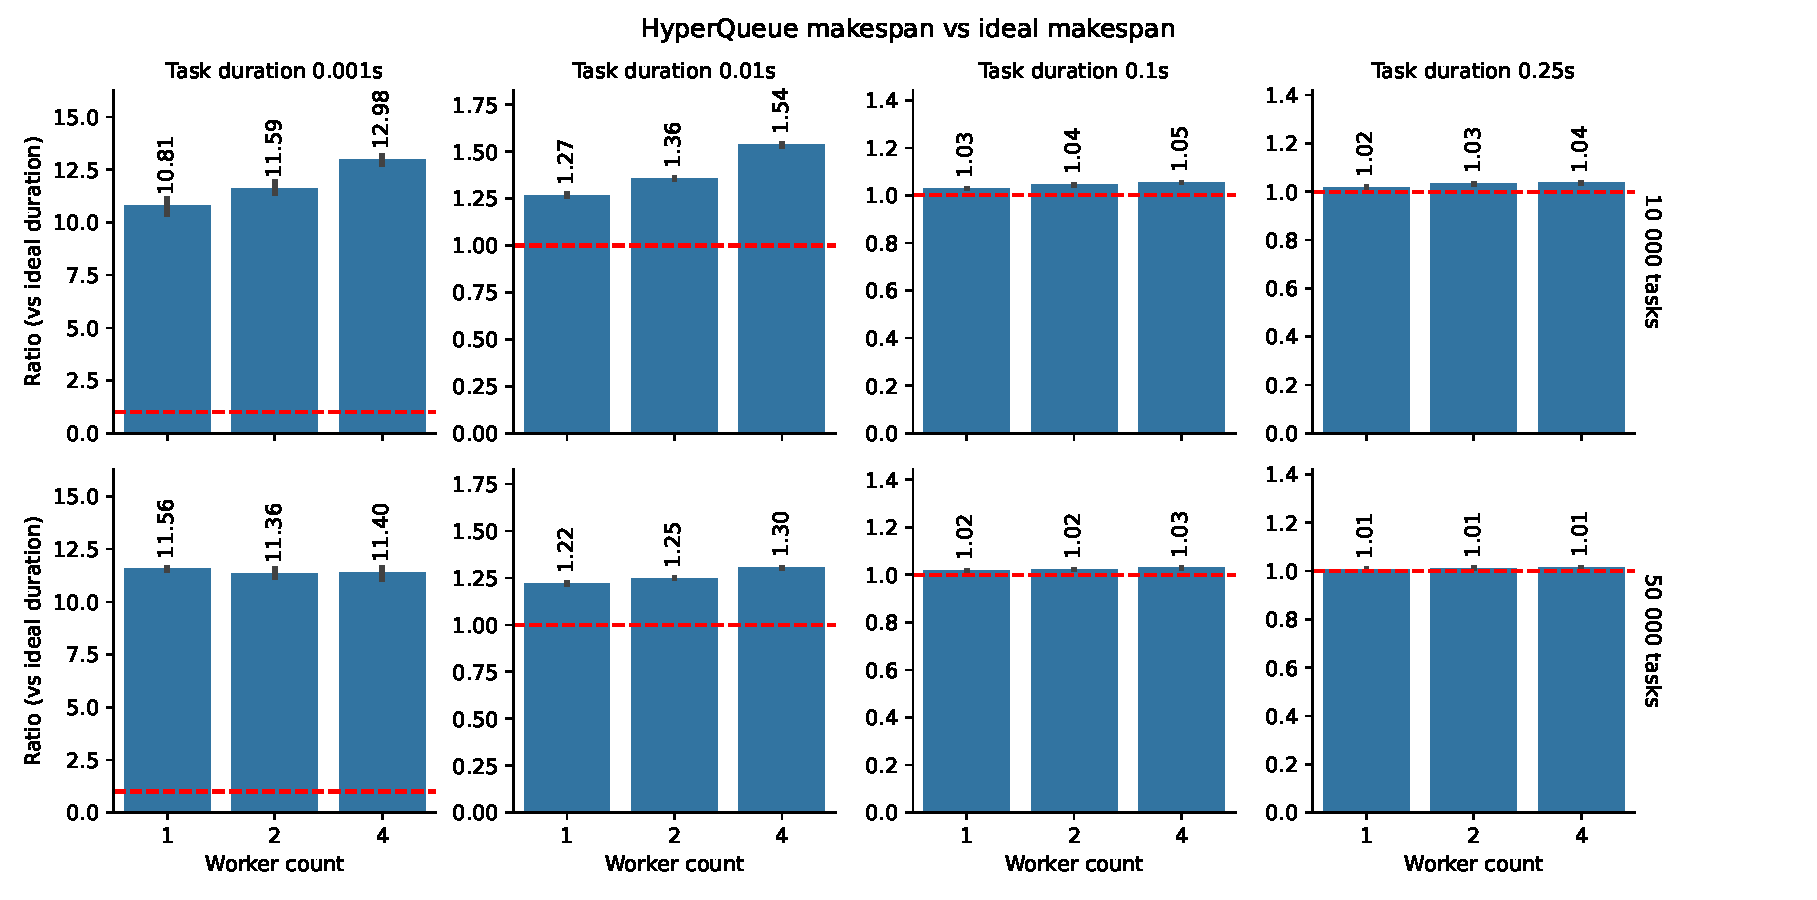
\includegraphics[width=\textwidth]{imgs/hq/charts/total-overhead-vs-ideal}
	\caption{Total overhead of \hyperqueue{} (ratio vs theoretically ideal makespan)}
	\label{fig:hq-overhead-vs-ideal}
\end{figure}

The results of this experiment can be observed in~\Autoref{fig:hq-overhead-vs-ideal}. Each chart column shows
a different task duration; the rows separate different task counts. Within each chart, the
horizontal axis represents the number of used workers, while the vertical axis shows the duration
needed to execute the task graph in \hyperqueue{}, normalized to the theoretical ideal
duration. The ideal duration is marked with a red horizontal dotted line. For example, the value
$1.05$ specifies that the \hyperqueue{} execution was
$5\%$ slower than the ideal duration.

We can see that for tasks that last for \SI{100}{\milli\second} or more, the overhead of
\hyperqueue{} is within $5\%$ of the ideal makespan; with the larger
task graph that contains $50$ thousand tasks, the overhead stays within
$3\%$. The overhead increases slightly with an added number of workers, which is
expected; the scheduler needs to perform more work and the server also communicates with more
workers over the network.

The situation becomes more interesting in the case where the task duration is only
\SI{1}{\milli\second}. Here the overhead of \hyperqueue{} seemingly becomes very large.
We have examined this situation in detail and found out that the issue is caused mostly by slow
command execution performance on Karolina. Our calculation of the theoretically ideal makespan
assumes that the executed command will last for exactly \SI{1}{\milli\second}. However, through
several benchmarks, we found out that running even the shortest possible process (that
immediately exits) on Karolina
takes \emph{at least}
\SI{500}{\micro\second}, and executing a program that is supposed to sleep for
\SI{1}{\milli\second} can take several milliseconds. Because the overhead of actually executing
the command is so large, it skews the total overhead of \hyperqueue{}, as it is not able
to reach the theoretically ideal makespan, because the execution of commands takes more time than
expected. Note that this would be an issue for any task runtime that executes a command in each
task, and there is not that much that \hyperqueue{} could do to avoid this overhead. We
eventually found out that the slow process spawning performance is caused primarily by an old
version of the \texttt{glibc} \texttt{C} standard library implementation used on Karolina; there
is not much that we could do about that.

\begin{figure}[h]
	\centering
	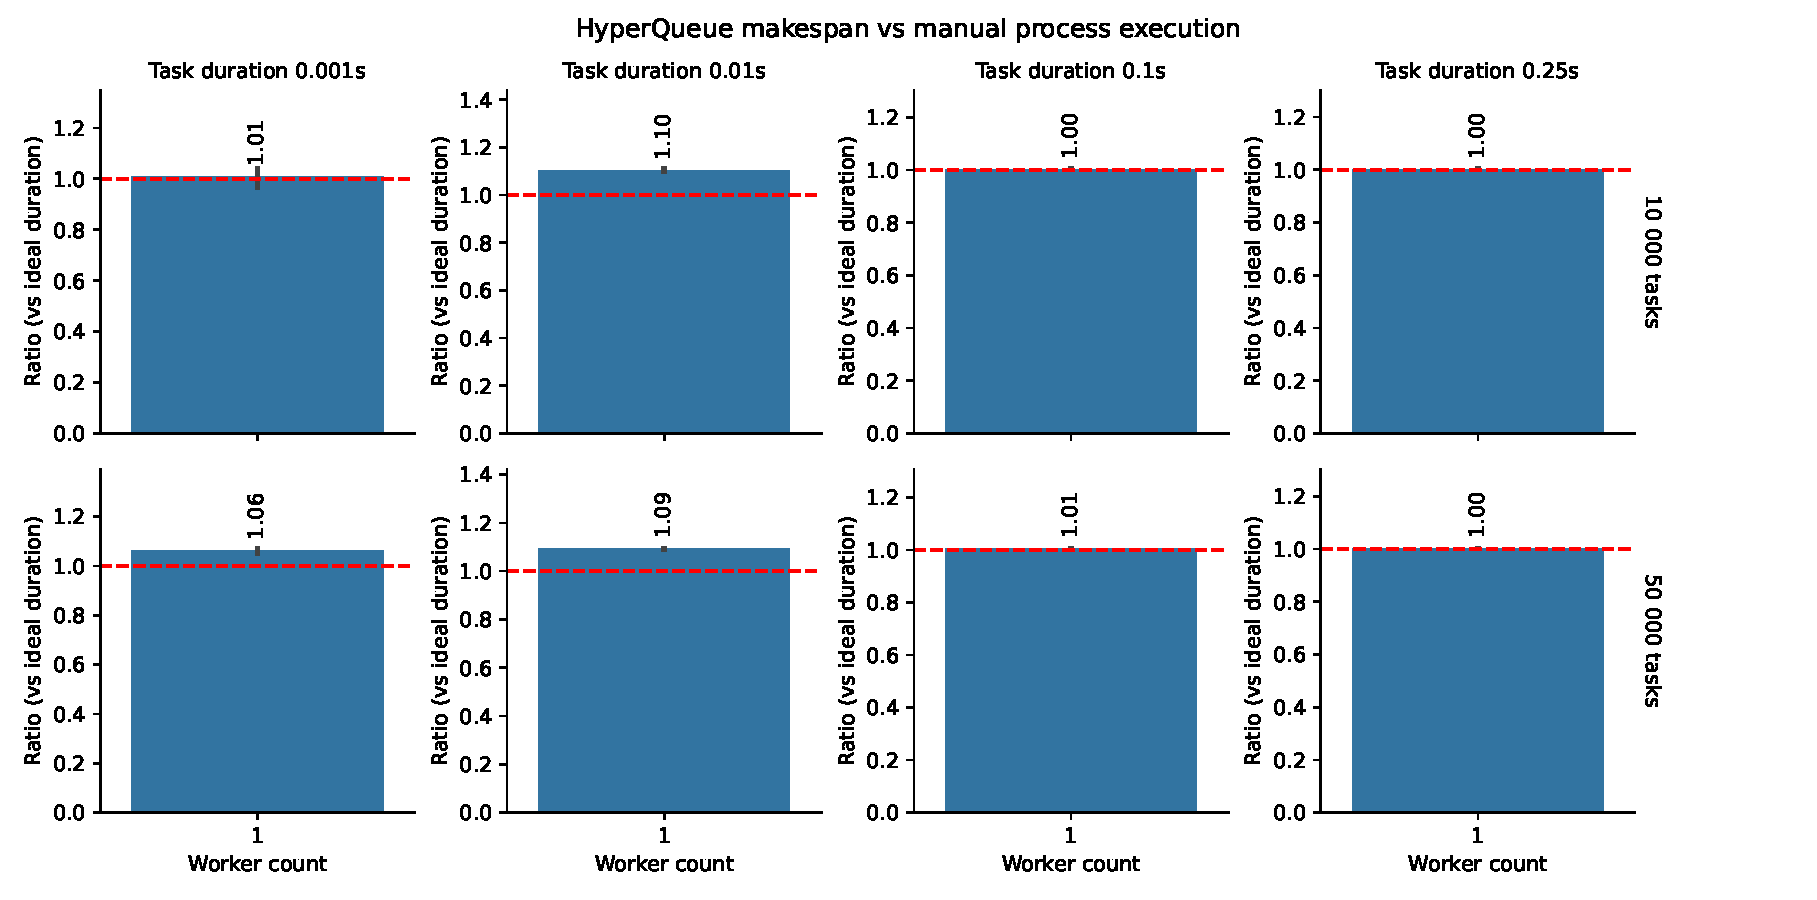
\includegraphics[width=\textwidth]{imgs/hq/charts/total-overhead-vs-manual}
	\caption{Total overhead of \hyperqueue{} (ratio vs manual process execution)}
	\label{fig:hq-overhead-vs-manual}
\end{figure}

To provide a fairer evaluation of the overhead of \hyperqueue{} for short tasks, we have
also evaluated it against a different baseline, which is not based on a theoretical calculation,
but on the actual performance of command execution on Karolina. We have implemented a simple
program that executes the same tasks (\texttt{sleep} processes) as
\hyperqueue{}, in parallel on all $128$ available cores. This provides a
more reasonable baseline that takes into account the overhead of command execution on Karolina. The
results of this experiments can be seen in~\Autoref{fig:hq-overhead-vs-manual}. The baseline is marked with a
horizontal red line; it represents the fastest measured time to execute the given number of
processes. We have performed this experiment only with a single worker, because our baseline
program did not implement multi-node distribution. Based on these results, we can see that for the
\emph{simple workflow}, the actual overhead of \hyperqueue{} (when compared to manually
running the commands without a task runtime) stays within $10\%$ even for very short tasks.

\subsection{Task throughput}
\label{sec:hq-exp-task-throughput}
The previous experiment has evaluated the total overhead of \hyperqueue{} while taking
into account the time to execute tasks. To further examine the inner overhead of scheduling and
network communication, in this experiment we evaluate the possible task throughput (number of tasks
processed per second) using the \emph{zero worker} mode. In this mode, \hq{}
performs all operations that it does normally (managing tasks and workers, scheduling, sending
network packets), but it does not actually execute the tasks; the corresponding worker immediately
marks each task as completed instead. This allows us to examine the overhead of
\hyperqueue{} without it being affected by process spawning, which can have severe
overhead, as was demonstrated in the previous experiment. We have benchmarked the
\emph{simple workflow} containing from $10$ thousand to $1$
million tasks with varying worker counts (up to $16$ workers and thus
$2048$ \gls{cpu} cores).

\begin{figure}[h]
	\centering
	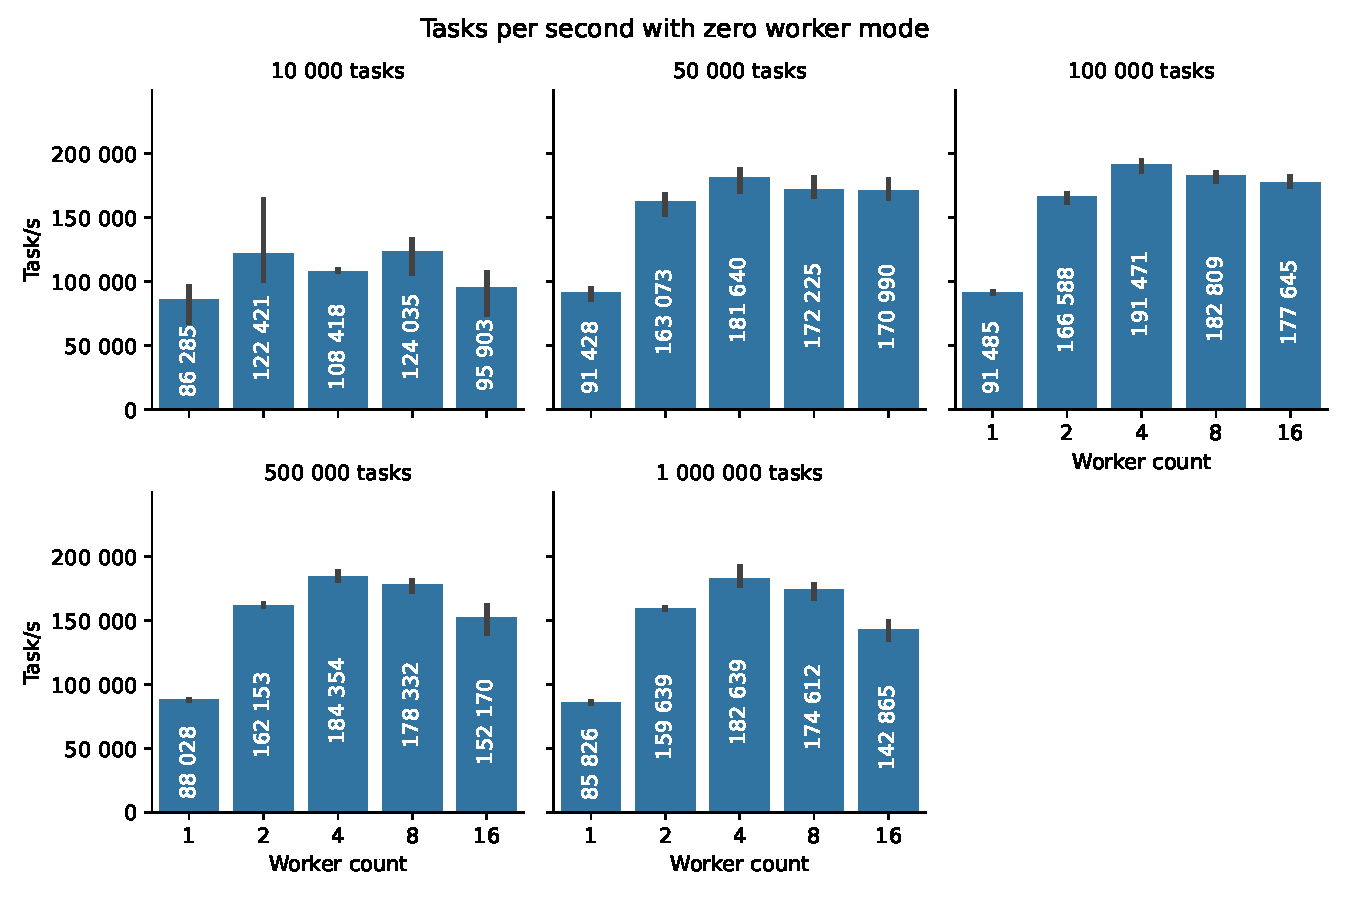
\includegraphics[width=0.8\textwidth]{imgs/hq/charts/task-per-s}
	\caption{Tasks processed per second with \emph{zero worker} mode}
	\label{fig:hq-tasks-per-s}
\end{figure}

The results can be observed in~\Autoref{fig:hq-tasks-per-s}. The horizontal axis displays the number of
workers in the task graph, while the vertical axis displays the achieved throughput measured in
tasks processed per second. In theory, the throughput should be increasing with more added workers. For
the smallest task graph with $10$ thousand tasks, the throughput increases up to
four workers ($512$ cores), then it decreases; the task graph is too small and the
constant overhead factors start dominating over the available parallelism. For task graphs with up
to $100$ thousand tasks, the throughput also increases up to four workers, where it
saturates. For even larger task graphs, the throughput once again starts decreasing with more than
four workers; the overhead of network communication and scheduling starts to dominate.

The absolute numbers of the achieved throughput demonstrate that \hyperqueue{} has very
little baseline overhead, and can in theory execute hundreds of thousands of tasks per second. The
tasks would have to be shorter than approximately \SI{5}{\micro\second} to fully saturate the
throughput achievable by \hyperqueue{}. Such a task duration is uncommon for scientific
workflows (indeed, on Karolina even starting a new process takes a hundred times longer); it is
more common for task-parallel programming models that have been described
in~\Autoref{sec:task-granularity}, which are operating on a very different level of granularity than what
\hyperqueue{} was designed for. This task throughput is orders of magnitude higher than
throughput measured for the \parsl{}, \fireworks{} and
\dask{} task runtimes, as reported in~\cite{parsl}.

As you may recall from~\Autoref{dask:evaluation}, the overhead per task of \dask{}
for a task graph with $50$ thousand tasks and a single node (using the
\emph{zero worker} mode) was approximately \SI{0.3}{\milli\second}. The per-task overhead of
\hyperqueue{} (calculated as an
inverted value of the number of tasks executed per second) for a similar configuration evaluated in this experiment is approximately
\SI{0.01}{\milli\second}, an order of magnitude lower.

\subsection{Strong scaling}
\label{sec:hq-exp-scalability}
This experiment evaluates the ability of \hyperqueue{} to scale to many computational
resources, by executing the same task graph with increasing worker counts (up to
$64$ workers and thus $8192$ cores in total). Note that each
benchmark configuration in this experiment was measured only once because of the large amount of
computational resources required to allocate tens of worker nodes.

We have designed two separate scenarios for this experiment. In the first one, we have selected a
fixed target makespan, so that the \emph{simple workflow} would be executed in approximately $5$
minutes ($300$ seconds) on a single worker, and benchmarked
three task graphs with increasing task counts. This allowed us to examine how the
scalability of \hyperqueue{} changes based on the number of tasks in the task graph when the total
computational workload stays the same. The task duration of each task was scaled accordingly for
each graph, so that the total makespan on a single worker would be $5$ minutes.
The benchmarked worker counts were $1$, $2$,
$4$, $8$, $16$, $32$
and $64$.

\begin{figure}[h]
	\centering
	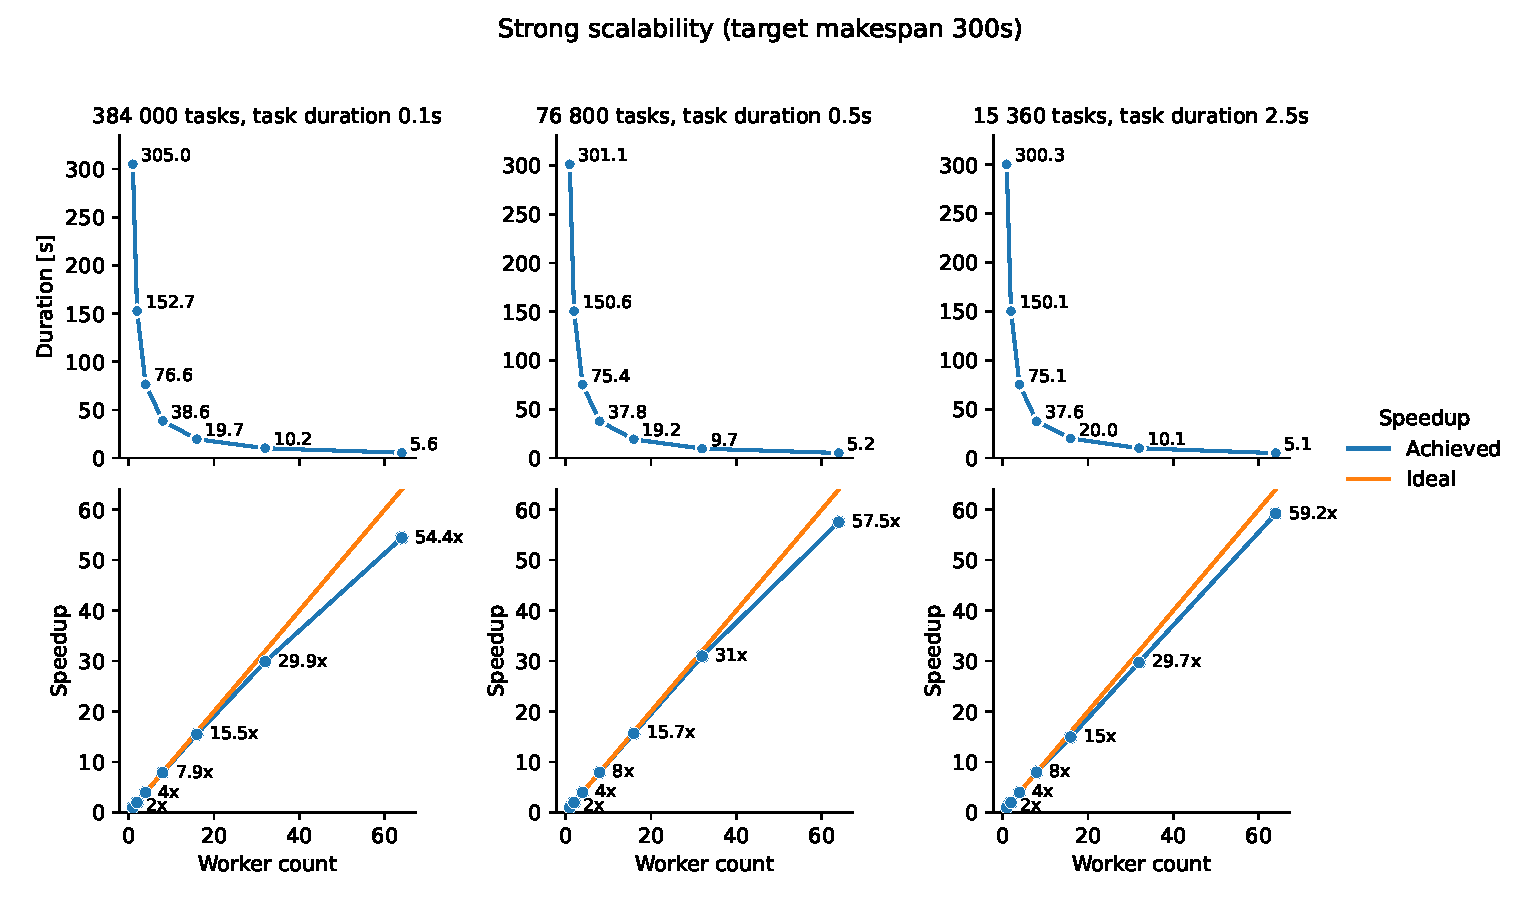
\includegraphics[width=\textwidth]{imgs/hq/charts/scalability-fixed-makespan}
	\caption{Strong scalability of \hyperqueue{} with a fixed target makespan
	(\SI{300}{\second})}
	\label{fig:hq-scalability-fixed-makespan}
\end{figure}

The results of the benchmark with a fixed makespan can be observed in~\Autoref{fig:hq-scalability-fixed-makespan}. The
horizontal axis displays the number of workers used for executing the task graph. In the top row,
the vertical axis shows the measured makespan; in the bottom row, the vertical axis shows speedup
against the measured makespan on a single worker. We can see that for all three measured task
durations, \hyperqueue{} was able to scale reasonably well up to $64$
workers, where it was able to compute the whole task graph in approximately $5$
seconds. In the best case, with tasks that took \SI{2.5}{\second} to execute, it provided a
$59.2$x speedup over a single worker using $64$ workers. In the worst case, with
tasks that lasted \SI{100}{\milli\second}, it provided a $54.4$x speedup over a single worker using
$64$ workers. With task duration \SI{0.1}{\second} and
$64$ workers, \hyperqueue{} was able to dispatch almost
$70$ thousand tasks per second.

In the second scenario, we fixed the task duration of each task to $1$ second
and then varied the task count. This allowed us to examine how the strong scalability of
\hyperqueue{} changes with an increasing number of tasks.

\begin{figure}[h]
	\centering
	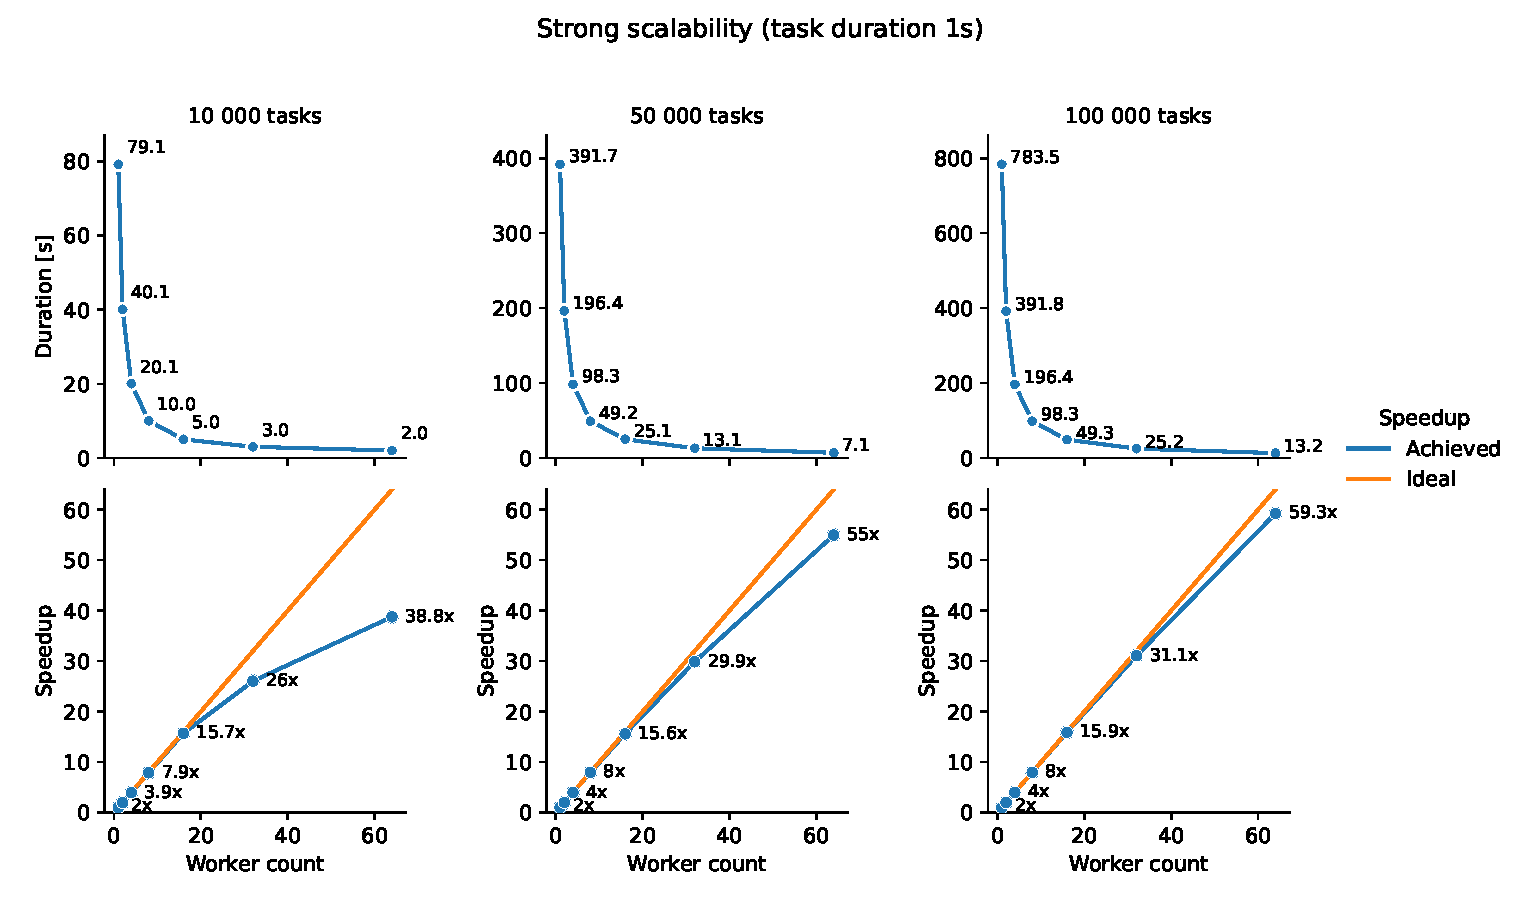
\includegraphics[width=\textwidth]{imgs/hq/charts/scalability-fixed-task-duration}
	\caption{Strong scalability of \hyperqueue{} with a fixed task duration (\SI{1}{\second})}
	\label{fig:hq-scalability-fixed-task-duration}
\end{figure}

We can observe the results in~\Autoref{fig:hq-scalability-fixed-task-duration}. We can see that the scalability improves
with the number of tasks; with $100$ thousand tasks, \hyperqueue{} is
able to provide a $59$x speedup with $64$ workers. On the
other hand, with only $10000$ tasks, the speedup in this case reaches only
$38.8$x, because there are not enough tasks to saturate all workers. With
$64$ workers that each have $128$ cores, the total number of
cores managed by \hq{} is $8192$. Therefore, each worker barely gets a single task to compute in
this small task graph.

In general, the results of our scalability and overhead experiments indicate that \hyperqueue{}
introduces very little overhead and is able to scale to a large amount of computational
resources (tens of nodes and thousands of cores) and also to large amounts of tasks
(hundreds of thousands) without an issue.

\subsection{Performance comparison of \dask{} and \hq{}}
\label{sec:hq-exp-dask}
This experiment evaluates basic performance differences between the \dask{} task
runtime and \hyperqueue{}. We have evaluated \emph{dask/distributed}
$2024.7.0$ running under CPython $3.10.8$ with a disabled monitoring
dashboard for improved performance. All measurements in this experiment were performed only once,
to reduce the required computational resources.

We have evaluated the scalability of both runtimes on the \emph{simple workflow} with a target
makespan set to \SI{30}{\second} on a single worker, with an increasing number of workers
and a varying number of tasks. In this scenario, \dask{} was benchmarked in three
separate worker configurations, with $1$ process per node and
$128$ threads per process ($1p/128t$), with $8$
processes per node and $16$ threads per process ($8p/16t$) and
with $128$ processes per node and $1$ thread per process
($128p/1t$). The reason for choosing different process/thread combinations has been
extensively explained in~\Autoref{dask:evaluation}; we chose two extremes ($1$
process and $128$ processes) and then a compromise with $8$
processes per node, according to recommendations in the \dask{}
documentation~\cite{dask-thread-recommendation}.

\begin{figure}[h]
	\centering
	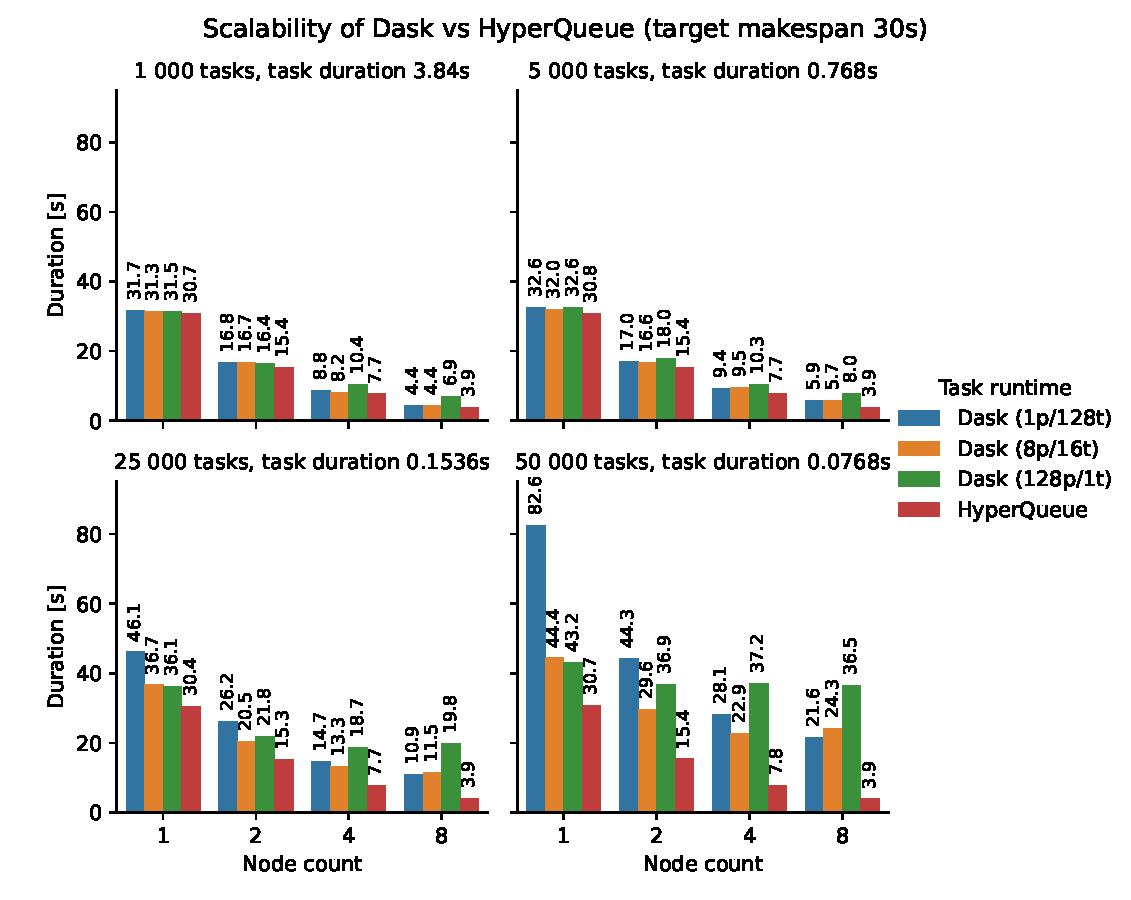
\includegraphics[width=0.8\textwidth]{imgs/hq/charts/dask-vs-hq-sleep}
	\caption{Scalability of \hyperqueue{} vs \dask{} with a fixed target makespan
	(\SI{30}{\second})}
	\label{fig:hq-dask-sleep}
\end{figure}

The results of this experiment are displayed in~\Autoref{fig:hq-dask-sleep}. The individual charts
display separate task graphs with varying task counts (in each case, the task graph should have a
makespan of $30$ seconds on a single node). The horizontal axis shows the amount
of used nodes and the vertical axis displays the makespan. Note that we are using the term
\emph{node count} instead of \emph{worker count} here, because each
\dask{} process spawned per node is technically a separate worker. We can see that
the in the case of \dask{}, the performance depends a lot on the number of tasks in
the task graph and also on the task duration. With only $1000$ tasks and task
duration in the range of seconds, \dask{} is able to scale relatively well in all
three configurations, although it is still slightly slower than \hyperqueue{}. However,
with a larger number of tasks (tens of thousands), and tasks that last only hundreds or tens of
milliseconds, the performance of \dask{} decreases very quickly.

We can also see differences between the three \dask{} configurations, particularly
in the benchmark with $50000$ tasks. With a single node, \dask{} is
unable to keep up with the number of tasks, and it has a twice longer makespan than when multiple
worker processes are used. On the other hand, once the number of nodes is increased, the situation
reverses, and the configuration with a single worker per node becomes the fastest one, because
\dask{} starts being overwhelmed by the number of connected workers. This suggests
that some amount of manual tuning based on the number of used nodes and workers might be required
to achieve optimal performance of \dask{} workflows. Conversely,
\hyperqueue{} was able to keep a consistent performance profile in this experiment
without being heavily affected by the number of tasks or the task duration. And because each
\hq{} worker manages all resources of its node, it does not require
any manual worker tuning.

Note that this benchmark actually presents a sort of a best-case scenario for
\dask{}. It executes its tasks as Python functions; therefore, it does not need to
start a new Linux process per task, unlike \hyperqueue{}. Furthermore, since each task
simply sleeps for a specified duration, it releases the \gls{gil} and thus does not
block other Python threads of the worker, which can thus perform other work concurrently.

\begin{figure}[h]
	\centering
	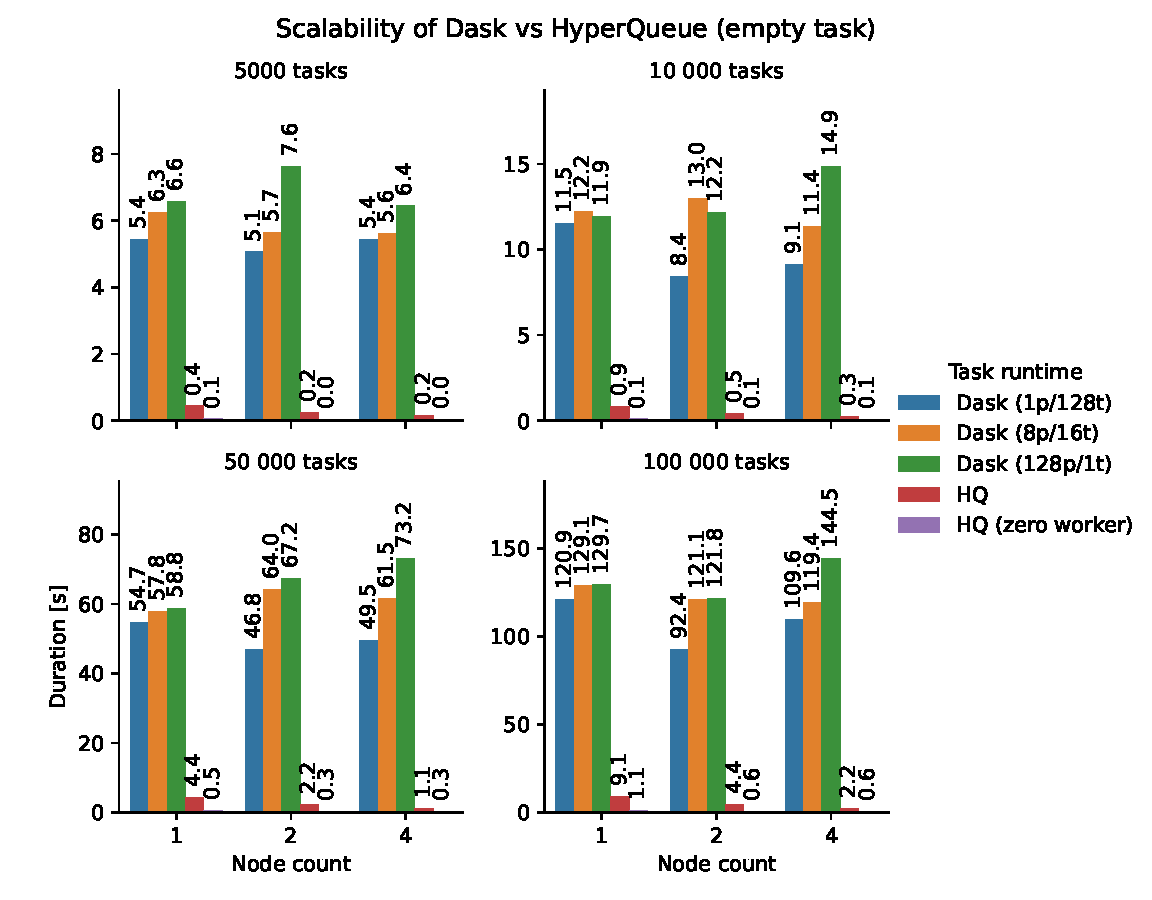
\includegraphics[width=0.8\textwidth]{imgs/hq/charts/dask-vs-hq-empty}
	\caption{Scalability of \hyperqueue{} vs \dask{} with an empty task}
	\label{fig:hq-dask-empty}
\end{figure}

We have further examined the baseline overhead of \dask{} by executing an empty
task (an empty Python function), which emulates the \emph{zero worker} mode of
\hyperqueue{}, as it shows how the task runtime scales with the fastest possible task
execution. We have compared this empty task execution with running the fastest possible task in
\hyperqueue{} (by spawning a process that immediately exits) and also with the \emph{zero worker} mode of \hyperqueue{}.

The results of this experiment can be seen in~\Autoref{fig:hq-dask-empty}. The horizontal axis shows
the node count and the vertical axis displays the makespan. Here we can observe a large difference
between the inner overhead of \hyperqueue{} and \dask{}, which struggles
to keep up with large amounts of very short tasks. This is of course an artificial scenario because
the tasks are empty; however, it does demonstrate that \dask{} can have
performance issues with large or very granular task graphs. It is also clear that the overhead of
\dask{} increases quickly with multiple added workers, which is further exacerbated
when multiple workers per node are used.

\subsection{Resource variants}
\label{sec:hq-exp-resource-variants}
This experiment evaluates the load-balancing benefits of \emph{resource variants}, which were
described in~\Autoref{sec:dynamic-resource-selection}. For evaluation, we use the simple workflow with
$300$ tasks executed on a single node with $8$ virtual
\glspl{gpu} and the same number of \glspl{cpu}. Tasks in this experiment
simulate a computation that can run either on a \gls{gpu} or on a
\gls{cpu}. To emulate the performance difference between the \gls{gpu}
and the \gls{cpu}, tasks executed on the accelerator will sleep for
\SI{1}{\second} and tasks executed on the \gls{cpu} will sleep for a
multiple of this duration, according to a given ratio (which is a benchmark parameter).
Note that we could also use a larger number of \gls{cpu} cores and reduce the benchmarked values
of this ratio; the result should be approximately the same.

Our goal was to determine how will the resulting makespan differ for the following three
situations:
\begin{itemize}[itemsep=0pt,topsep=2pt]
	\item Tasks are executed only on the \gls{gpu}.
	\item A fixed fraction of tasks is executed on the \gls{gpu}, the rest runs on the
	      \gls{cpu}.
	\item The fraction of tasks that is executed on the \gls{gpu} is determined dynamically by
	      \hyperqueue{} using resource variants.
\end{itemize}

\begin{figure}[h]
	\centering
	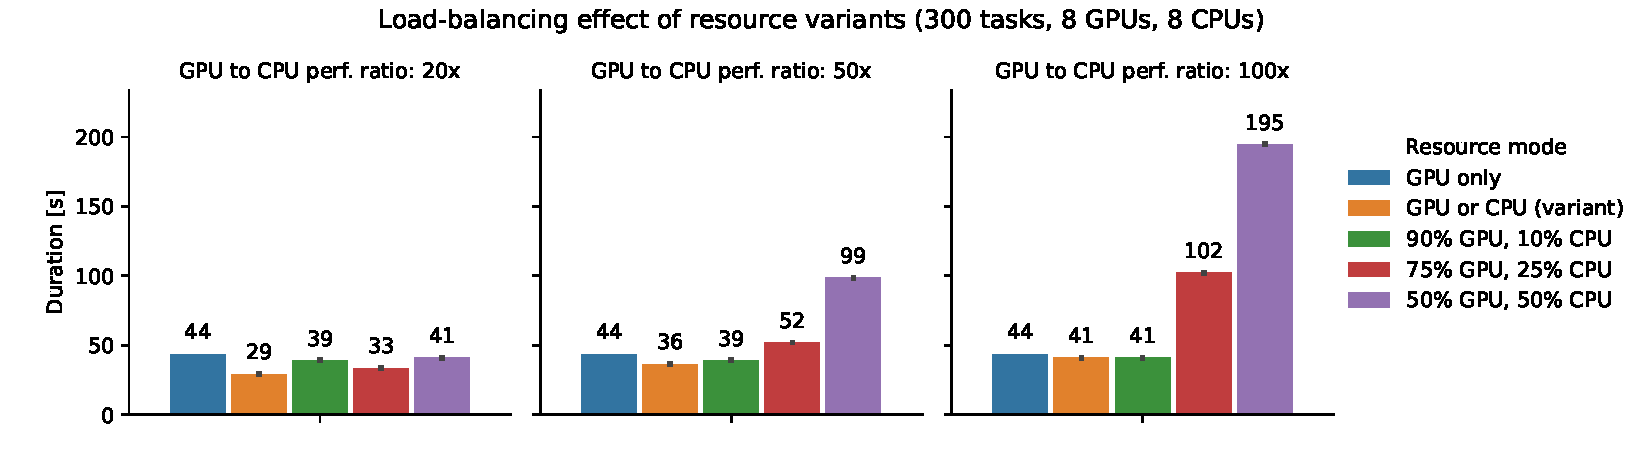
\includegraphics[width=\textwidth]{imgs/hq/charts/alternative-resources}
	\caption{Load-balancing effect of resource variants}
	\label{fig:hq-resource-variants}
\end{figure}

\vspace{1mm}The results of the experiment can be observed in~\Autoref{fig:hq-resource-variants}.
The vertical axis displays the makespan; the five bars represent different configurations of resources. In the
\emph{\gls{gpu} only} mode, all tasks were configured to run on a single
\gls{gpu}. In the \emph{\gls{gpu} or \gls{cpu}} mode, tasks were configured to run either
on the \gls{gpu} or on the \gls{cpu} using resource variants. The
remaining three modes assign a specific fraction of tasks to run on the \gls{gpu};
the rest was executed on the \gls{cpu}. The three charts show results for different
values of the \gls{gpu} vs \gls{cpu} performance ratio, i.e.\ how much
faster was the task running on a \gls{gpu} than on the \gls{cpu}.

We can see that unless the \gls{gpu} ratio is too high or we assign too many tasks to
the \gls{cpu}, it is beneficial to also leverage the \gls{cpu}
resources rather than using only \glspl{gpu}. With \gls{cpu} fractions
determined manually in advance, the result depends heavily on the \emph{\gls{gpu} ratio}, and in
certain configurations it can make the makespan significantly longer. This would thus be both less
efficient and more laborious to configure for the user. On the other hand, when the resources for
each task are configured using two resource variants (either \gls{gpu} or
\gls{cpu}), \hyperqueue{} is able to dynamically adapt to all three
\gls{gpu} ratios. In all three scenarios, the makespan with resource variants is
strictly smaller than with \glspl{gpu} only, and it either surpasses or matches the
best result achieved with a predetermined fraction of tasks running on the \gls{cpu}.
This shows that resource variants can help achieve better hardware utilization without requiring
the user to fine-tune resource configurations of individual tasks in the task graph.

\subsection{Group allocation strategies}
\label{sec:hq-exp-numa}
This experiment examines the effect of resource group allocation strategies on the
performance of programs that are sensitive to memory latency. Each Karolina
\gls{cpu} (non-accelerated)
computational node has $128$ cores and \SI{256}{\gibi\byte} of memory, divided
into $8$ \gls{numa} nodes. Accessing memory across these
\gls{numa} nodes is slower than accessing memory within the same node, which can
affect the performance of programs that are very sensitive to memory throughput or latency. We have
created a simple program inspired by the STREAM benchmark~\cite{stream} that exerts this
behavior; it is very sensitive to \gls{numa} memory placement. First, it allocates and
initializes \SI{4}{\gibi\byte} of memory stored in a single \gls{numa} node.
Then, a number of threads pinned to individual cores repeatedly read from this memory in turn. When
these threads are running on cores from a different \gls{numa} node than where the memory was
allocated, the program takes longer to execute due to memory transfers being slower.

We have benchmarked the \emph{simple workflow} with $100$ tasks on a single
Karolina node, where each task executes the described program with either $4$
or $8$ threads (cores). Each task is configured so the spawned threads are
pinned to the specific set of cores assigned to that task by the
scheduler. Each available group allocation strategy was
examined; \emph{Compact}, which tries to allocate cores using the smallest possible
number of groups, \emph{Strict compact}, which always draws cores from the smallest possible
number of groups and \emph{Scatter}, which attempts to allocate cores across different groups.
As you may recall,
\hyperqueue{} workers by default separate available cores into groups according to their
\gls{numa} node. We also evaluate another option, \emph{No strategy}, which
emulates the behavior of task runtimes that do not provide support for managing groups or
\gls{numa} nodes. In this strategy, workers are configured with a flat set of
\gls{cpu} cores without any groups. The order of the available cores is also
randomized so that the scheduler cannot use any knowledge of which tasks belong to the same
\gls{numa} node.

\begin{figure}[h]
	\centering
	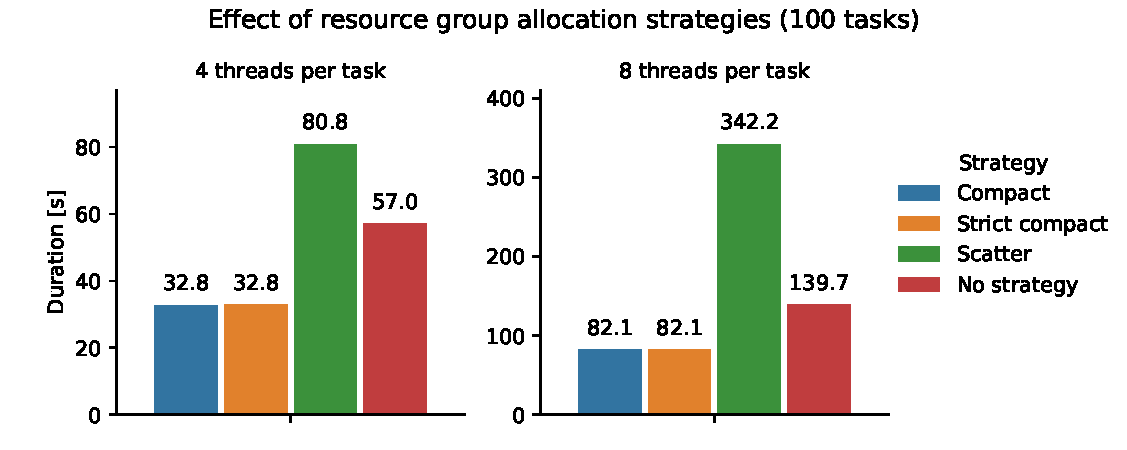
\includegraphics[width=0.8\textwidth]{imgs/hq/charts/numa}
	\caption{Effect of different group allocation strategies}
	\label{fig:hq-numa}
\end{figure}

We can observe the results of this experiment in~\Autoref{fig:hq-numa}. The vertical axis displays
the makespan of the executed task graph and the four bars represent results of individual
strategies. For both evaluated core counts per task, the best performance was achieved using the
\emph{Compact} strategy, because the threads were able to achieve the highest possible
memory throughput. The \emph{Strict compact} strategy achieved essentially the same result;
because the task durations were quite uniform, these two strategies resulted in very similar
placements of cores to tasks. On the other hand, the \emph{Scatter} strategy resulted in
the worst possible performance, as expected. The results of the \emph{No strategy}
configuration are perhaps the most interesting. When cores were assigned to tasks essentially at
random, without taking \gls{numa} effects into account, the performance was better
than with the \emph{Scatter} strategy, because in some cases the tasks received multiple
cores belonging to the same \gls{numa} node. However, it was still almost twice as
slow than with the \emph{Compact} strategy. This suggests that for memory-sensitive
programs, using a \gls{numa}-aware task allocation strategy can significantly improve
the achieved performance.

\subsection{Worker \glsxtrshort{cpu} utilization}
\label{sec:hq-cpu-utilization}
One of the primary metrics that task graph users care about is hardware utilization -- how well can
a task graph (executed with a given task runtime) make use of available resources? This experiment
examines the average \gls{cpu} utilization of worker nodes while executing a task
graph with \hyperqueue{}, both for tasks with a uniform duration and also for tasks with
a skewed distribution of durations. We have benchmarked the \emph{simple workflow} with
$10$ thousand tasks, where each task fully utilizes a full
\gls{cpu} core by executing the \texttt{stress} UNIX utility (instead of just
sleeping). This task graph was executed on four workers whose
\gls{cpu} utilization was periodically measured over the course of the computation.

\begin{figure}[h]
	\centering
	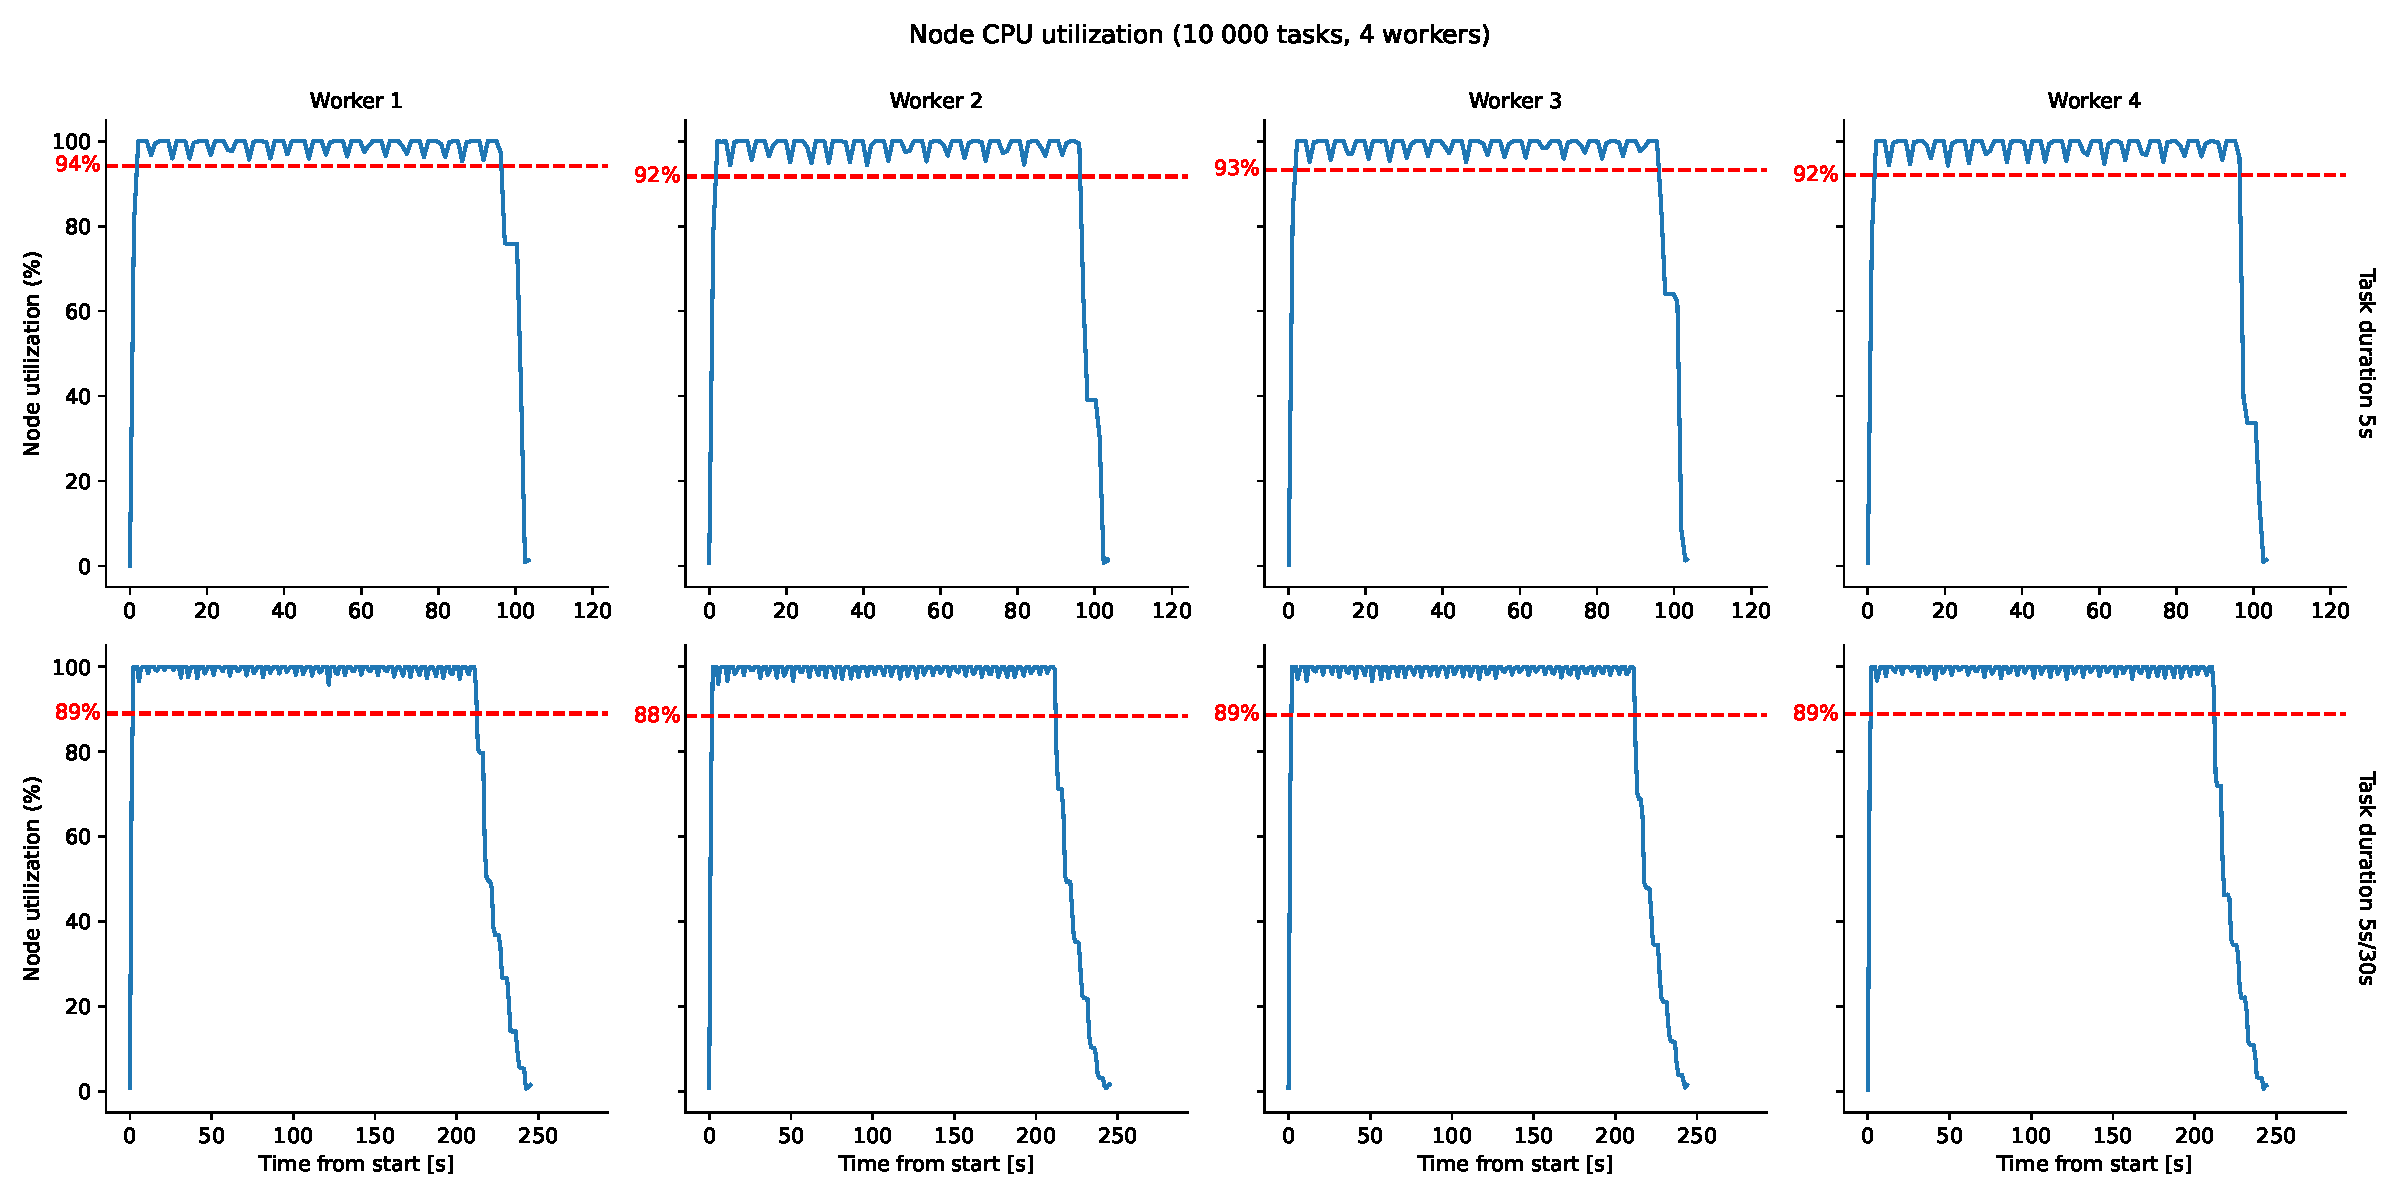
\includegraphics[width=\textwidth]{imgs/hq/charts/scalability-stress-utilization}

	In the bottom row, 75\% of tasks last \SI{5}{\second}, 25\% of tasks last
	\SI{30}{\second} \caption{\glsxtrshort{cpu} utilization of \hyperqueue{} worker nodes} \label{fig:hq-cpu-utilization}
\end{figure}

The results are shown in~\Autoref{fig:hq-cpu-utilization}. The horizontal axis shows the progress of the
computation in seconds, the vertical axis displays the average \gls{cpu} utilization
over all $128$ cores for each separate worker. The red horizontal dotted line marks the
total average utilization of each worker over the course of the whole computation. The top row
displays a situation where all tasks in the task graph have a uniform duration of
$5$ seconds. In this case, \hyperqueue{} workers kept their average
utilization at or above $92\%$. Note that it takes some amount of time for each
\texttt{stress} invocation to fully reach full core utilization, and since all tasks have
the same duration, the tasks perform this ramp-up process in a mostly synchronized fashion. This
causes the ``teeth'' in the utilization chart. Therefore, it is not realistic to reach full
$100\%$ node utilization with this task graph.

The second row displays a situation where the workload is skewed. Most ($75\%$) of
the tasks still have a duration of \SI{5}{\second}; the remainder simulates a ``long tail''
of slower tasks that take \SI{30}{\second} to execute. This is a more difficult situation
for achieving high utilization; because some tasks are longer, they might get stuck executing at a
time when other resources can no longer be utilized. We can observe this towards the end of the
workflow execution, where approximately $30$ seconds before the end, the
utilization starts to drop. However, even for this skewed task graph, the average
\gls{cpu} utilization of all four workers was kept at almost $90\%$.

\subsection{Server \glsxtrshort{cpu} consumption}
\label{sec:hq-exp-server-cpu-consumption}
When deployed on supercomputers, the \hyperqueue{} server is primarily designed to be
executed on their login nodes. This could pose a problem if it consumed too many system
resources, because login nodes are shared by multiple users and they are not designed for
computationally intensive tasks. Some clusters even forcefully limit the total amount of
\gls{cpu} time that can be consumed by processes running on login
nodes~\cite{leonardo_time_limit} and terminate the process if it exceeds the maximum allowed time.

To evaluate how many resources the server consumes, we have performed an experiment where the
server had to schedule a large number of tasks in a short time period (which acts as a sort of a
stress test); we have measured its total \gls{cpu} time consumption across all cores over this
period. The server was running on a login node and it was managing up to $12$ workers
($1536$ cores) and up to $200$ thousand tasks. Each worker was
deployed on a computational node, so that the server had to communicate with the workers over the
network. The benchmark was executed with a fixed makespan; the duration of each task was scaled so
that the whole task graph would finish computing in one minute. We measured the total amount of
\gls{cpu} time consumed by the server (both in user-space and in the kernel), using
standard Linux process monitoring tools.

\begin{figure}[h]
	\centering
	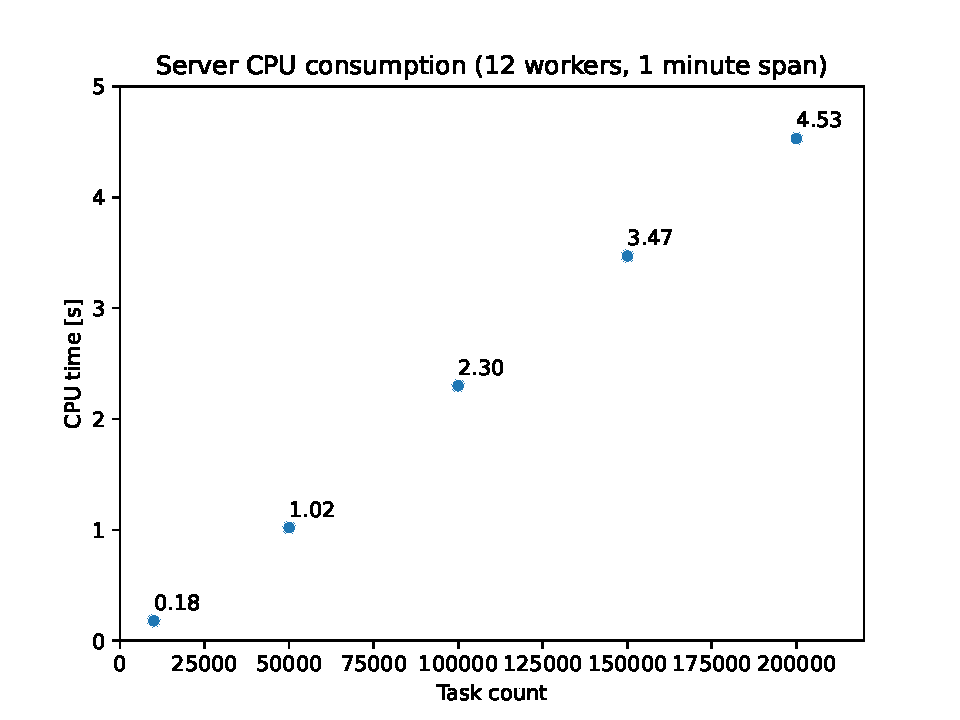
\includegraphics[width=0.6\textwidth]{imgs/hq/charts/server-utilization-tasks}
	\caption{\hyperqueue{} server \glsxtrshort{cpu} time consumption with an increasing number
	of tasks}
	\label{fig:hq-server-cpu-consumption-tasks}
\end{figure}

\Autoref{fig:hq-server-cpu-consumption-tasks} shows how the \gls{cpu} utilization of the
server changes with a fixed number of workers ($12$) and an increasing number of
tasks. In this case, the server had to schedule the \emph{simple workflow} with the number of tasks
ranging from $10$ to $200$ thousand. The horizontal axis shows
the number of tasks that were used for the given benchmark run and the vertical axis shows the
\gls{cpu} time consumed by the server over the measured one-minute period. We can see that the
amount of \gls{cpu} resources scales approximately linearly with the number of tasks
scheduled by the server. In the worst case, the server has consumed less than five seconds of
\gls{cpu} time over one minute of real time, even though it had to schedule
$200$ thousand tasks within this short period, which is an extreme stress test
that far exceeds the rate of scheduled tasks in most scientific workflows. Over all the benchmarked
task counts, the average \gls{cpu} consumption of the server per second and per
$1000$ tasks was approximately \SI{0.0003}{\second}. In other words, for every
thousand tasks in the task graph, the server consumed approximately \SI{0.3}{\milli\second}
\gls{cpu} time every second.

\begin{figure}[h]
	\centering
	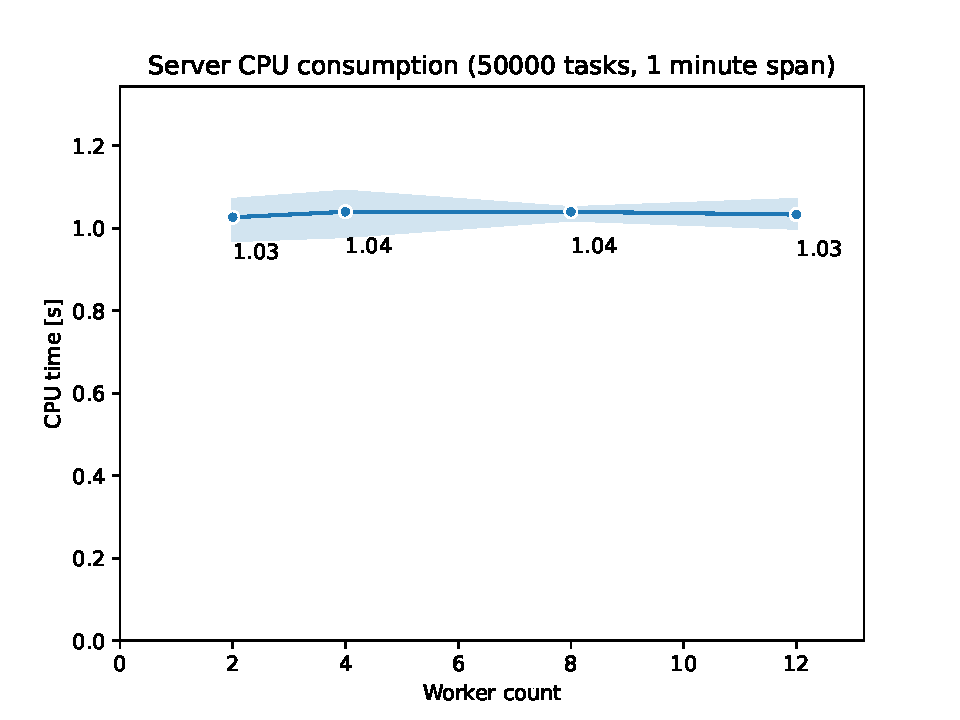
\includegraphics[width=0.6\textwidth]{imgs/hq/charts/server-utilization-workers}
	\caption{\hyperqueue{} server \glsxtrshort{cpu} time consumption with an increasing number
	of workers}
	\label{fig:hq-server-cpu-consumption-workers}
\end{figure}

\Autoref{fig:hq-server-cpu-consumption-workers} displays a situation where the number of tasks
is fixed ($50000$), but the number of workers increases from
$2$ to $12$. The horizontal axis shows the number of workers
that were used for the given benchmark run and the vertical axis shows the \gls{cpu}
time consumed by the server over the one-minute period. In this case, the consumption of the server
does not increase by a large amount with more added workers.

In terms of memory consumption, in the largest evaluated case with a task graph containing
$200$k tasks, the memory consumption of the server, measured using the Linux
\gls{rss} metric, was approximately \SI{120}{\mebi\byte}, which shows that the server
also does not consume large amounts of memory.

The amount of used resources will of course vary based on the executed workflow. However, this
experiment shows that the server consumes very few resources in general and that it still has a
lot of leeway available even if some task graphs proved to be more computationally demanding than
the benchmarked stress test.

\subsection{Encryption overhead}
\label{sec:hq-exp-encryption-overhead}
As has already been noted in~\Autoref{hq:architecture}, \hyperqueue{} encrypts all network
communication between the server, the workers, and the client. This encryption is performed because
the server is typically deployed on a login node, and thus the communication it performs can be in
theory observed by other users of the cluster. In this experiment, we have evaluated the overhead
of the encryption, by benchmarking \hyperqueue{} both with encryption enabled and
disabled.

We have benchmarked three instances of the \emph{simple workflow} containing
$10$, $50$ and $100$ thousand tasks executed
with four \hyperqueue{} workers in two configurations; with and without the
\emph{zero worker} mode. Because the \emph{zero worker} mode does not actually execute
any tasks, it emphasizes the inner overhead of \hyperqueue{} and should thus also amplify
potential differences in communication overhead caused by the encryption. Without the
\emph{zero worker} mode, each task simply executed the shortest possible sleep command, i.e.\
\texttt{sleep 0}.

\begin{figure}[h]
	\centering
	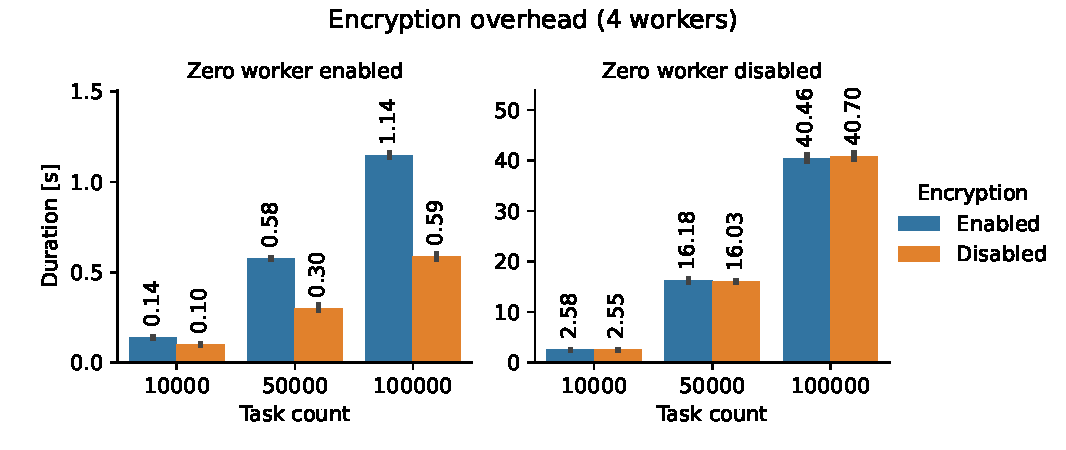
\includegraphics[width=0.8\textwidth]{imgs/hq/charts/encryption-overhead}
	\caption{Overhead of encryption in \hyperqueue{} communication}
	\label{fig:hq-encryption-overhead}
\end{figure}

We can observe the results of the experiment in~\Autoref{fig:hq-encryption-overhead}. The horizontal axis shows
the number of tasks in the benchmarked task graph and the vertical axis shows the
\emph{makespan}. In the \emph{zero worker} mode (displayed on the left), it is clear
that encrypting the communication in fact produces a measurable overhead. In the largest measured
case with $100$ thousand tasks, the makespan is approximately twice longer with
encryption enabled. However, as soon as the tasks do any actual work (albeit it being the simplest
work possible), the encryption overhead is no longer noticeable and it does not affect the total
makespan of the task graph.

In more realistic workflows, the executed tasks will be almost certainly longer than just executing
the trivial~\texttt{sleep} command. In that case, the overhead of encryption will be even
less noticeable; the larger the duration of the executed tasks, the less important is the overhead
introduced by \hyperqueue{}. If some users would still not want to use encryption for
some reason, \hyperqueue{} could be easily modified to add the option to disable
encryption at runtime.

\subsection{Output streaming}
\label{sec:hq-exp-output-streaming}
In this experiment we evaluate the effect of the \emph{output streaming} mode, which can be used to
stream the outputs of \emph{stdout} and \emph{stderr} streams from individual
tasks to the \hyperqueue{} server, to avoid creating a large number of files on the
filesystem. We have benchmarked two task graphs without dependencies, with $10$
and $50$ thousand tasks, where each task generates a fixed amount of data
($10$ or \SI{100}{\kibi\byte} per task). Each task simply outputs the
corresponding amount of data to its standard output (\emph{stdout}). The standard error
output is disabled and no output is printed to it. In the largest configuration, the task graph
produces approximately \SI{5}{\gibi\byte} of data in total.

With output streaming enabled, each task output is streamed to the server, which stores all data
sequentially into a single log file. Without output streaming, each task simply creates a single
file on disk and writes its \emph{stdout} output to it. The experiment was performed on
two different filesystem partitions of the Karolina cluster. The first partition, called SCRATCH,
uses the Lustre networked filesystem, which is designed for parallel high intensity
\gls{io} workloads~\cite{karolina_scratch}. It is a representative of a
high-performance filesystem; it can in theory reach up to \SI{700}{\gibi\byte}/s write
throughput. The second partition, called PROJECT, uses \gls{gpfs}, which is a much
slower filesystem implementation that focuses on providing high availability and
redundancy~\cite{karolina_project}.

\begin{figure}[h]
	\centering
	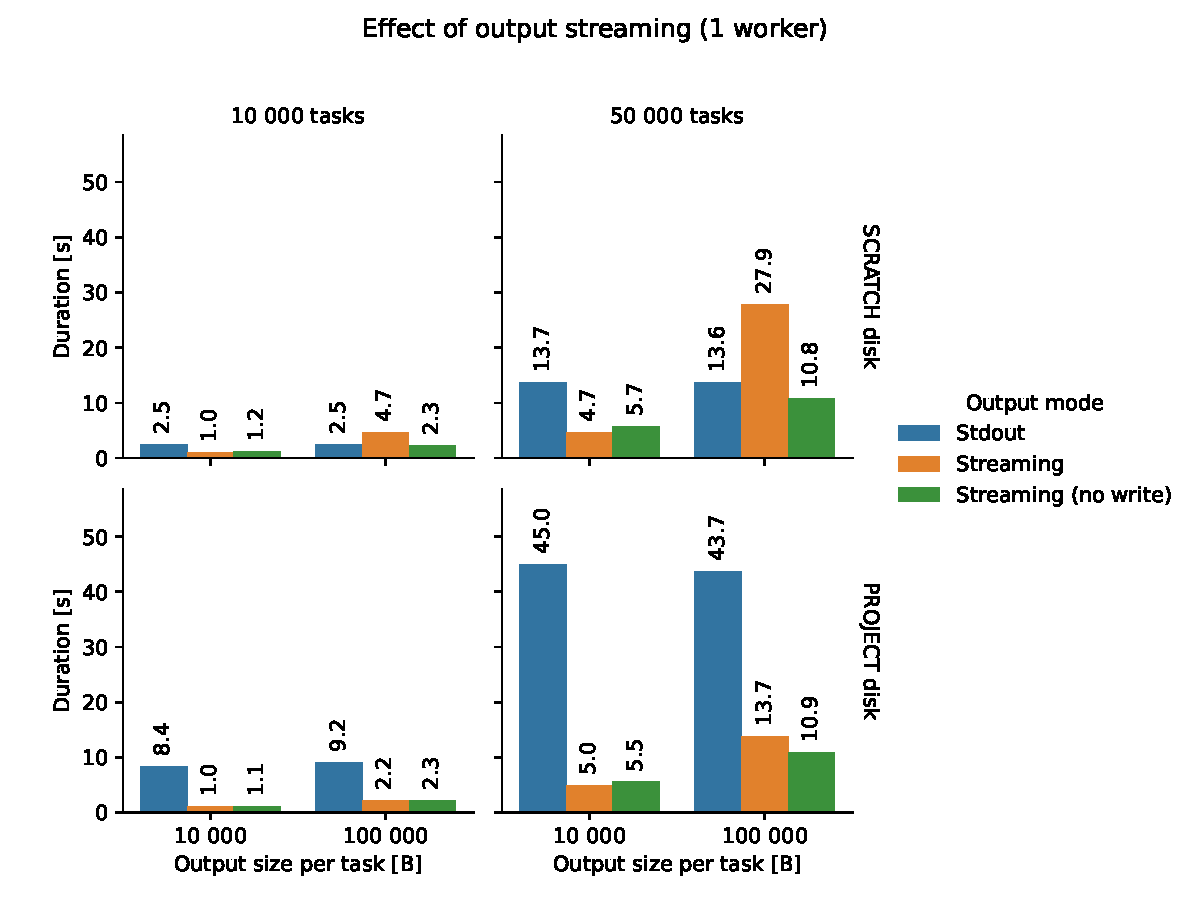
\includegraphics[width=0.7\textwidth]{imgs/hq/charts/io-streaming}
	\caption{Effect of output streaming on the makespan of tasks}
	\label{fig:hq-io-streaming}
\end{figure}

We can see the results of the experiment in~\Autoref{fig:hq-io-streaming}. The horizontal axis displays
the amount of output produced by each task and the vertical axis shows the makespan of the executed
task graph. The top row contains data for the SCRATCH filesystem; the bottom row contains data for
the PROJECT filesystem. Three separate configurations are displayed in the chart. In the
\emph{Stdout} mode, the task graph was executed without output streaming, while in the
\emph{Streaming} mode, the task graph was executed with output streaming. The third mode
will be described later below.

The results differ significantly based on the amount of output produced by each task and also based
on the used filesystem. On the SCRATCH Filesystem, output streaming was able to reduce the makespan
approximately by a half in the case where each task outputted \SI{10}{\kibi\byte} of data.
However, when the task output was larger (\SI{100}{\kibi\byte}), the situation reversed, and
output streaming became slower. This is most likely caused by the fact that the sequential writing
into the log file by the server becomes a bottleneck, as it cannot be easily parallelized by the
filesystem (unlike e.g.\ writing to many files in parallel). We have confirmed this by benchmarking
a third mode, which we call \emph{Streaming (no write)}. In this configuration, output streaming was
enabled; therefore, the output of tasks was streamed over the network from workers to the server,
but then the server simply discarded the data and did not write it to the sequential log file. We
can see that without actually sequentially writing the data to the log file, the makespan is still
shorter than without output streaming. It is thus clear that the primary bottleneck in this case is
in fact the final write to the log file.

It should be noted that even though output streaming is slower in this case, it still provides the
primary benefit of generating only a single file on the filesystem. It can thus help alleviate disk
quota limits without any user effort.

With the PROJECT filesystem, output streaming is $4$--$8$
times faster than writing to files directly. The performance benefit of output streaming thus
depends heavily on the used filesystem; it seems to be particularly helpful on slower filesystems.
One interesting result is that output streaming is generally faster on the PROJECT filesystem than
on the SCRATCH filesystem (even though the PROJECT filesystem itself should be much slower). Our
conjecture is that this might be caused by the network topology of the cluster. The SCRATCH
filesystem uses the InfiniBand~\cite{infiniband} network connection, which is also used for
network communication between the server and the workers; therefore, performing file
\gls{io} on the SCRATCH filesystem while also sending many network packets might
cause network contention.

\begin{table}[h]
	\centering
	\begin{tabular}{|r|r|r|r|r|}
		\hline
		Output per task [B] & Task count & Size (stream) [MiB] & Size (stdout) [MiB] & Ratio \\ \hline
		10000               & 10000      & 96                  & 118                 & 1.23x \\ \hline
		10000               & 50000      & 479                 & 589                 & 1.23x \\ \hline
		100000              & 10000      & 955                 & 978                 & 1.02x \\ \hline
		100000              & 50000      & 4775                & 4916                & 1.03x \\ \hline
	\end{tabular}
	\caption{Size of task output on disk with and without I/O streaming}
	\label{tab:hq-io-streaming-size}
\end{table}

Using output streaming has one additional advantage; it can reduce the total amount of consumed
disk space, because it creates only a single file on disk per job. On most filesystems, every file
occupies at least a single disk block (which typically consumes several KiB of space); therefore,
creating a large number of files also increases disk usage in general.~\Autoref{tab:hq-io-streaming-size}
shows the total size of the output of all tasks of the benchmarked task graphs on disk. The
\emph{Size (stream)} column shows the final size of the sequential log file (in this case,
output streaming was used), the \emph{Size (stdout)} column displays the total size of a
directory containing all files with outputs of individual tasks (in this case, output streaming was
not used) and the \emph{Ratio} column shows how much larger was the output in the case
where streaming was not used. In the case where each task has outputted \SI{10}{\kibi\byte} of
data, writing the output to individual files on disk resulted in approximately
$23\%$ higher disk usage. In the second configuration, where each task has
outputted \SI{100}{\kibi\byte} of data, this difference was reduced to $3\%$,
because the disk space overhead of file metadata became dwarfed by the size of their content.

Output streaming can help users avoid disk quota limits, reduce consumed disk space and in certain
situations also help with \gls{io} performance. However, it is also clear that
streaming so much data to a single location (the server) can be slower than writing to many files
in parallel if the given filesystem is optimized for such a use-case. As a future improvement,
streaming could be made more scalable by streaming task outputs to a single file (or a small amount
of files) \emph{per worker}, in order to distribute the \gls{io} load; outputs
from individual worker log files could then be merged by the server on demand.

\subsection{LiGen virtual screening workflow}
\label{sec:hq-exp-ligen}
This experiment evaluates the achieved hardware utilization and scalability of the LiGen virtual
screening workflow implemented using \hyperqueue{}. As explained previously
in~\Autoref{sec:hq-usecase-ligen}, the workflow uses a SMILES file as its main input, which contains a
description of a single ligand on each line. To allow \hyperqueue{} to balance the load
of the computation across available resources and nodes, the workflow first splits the single input
file into several smaller subfiles, each containing a subset of the input lines. Each such file is
then processed in two tasks; the first expands the ligands into a three-dimensional structure
stored in a MOL2 file and the second performs scoring on this expanded representation, which
generates a \gls{csv} file. All the intermediate \gls{csv} files are
then combined with a single final task at the very end of the workflow.

The number of ligands per file and the number of threads that are used for performing scoring on
each file are configurable parameters. There are various trade-offs associated with setting these
parameters. The expansion part is sequential; therefore, using as many files (tasks) as possible
for this step is beneficial up to the number of available cores. On the other hand, each scoring
invocation of LiGen for a file has a non-trivial cost, as it needs to perform a preprocessing step
and a part of the computation is also performed sequentially. Therefore, for the scoring part,
using fewer files is generally a better choice. Yet, with fewer files, there will also be less
opportunities for load balancing performed by \hq{} and there might not be enough
tasks to saturate the available computational resources.

We examine the effect of these two parameters on makespan and the achieved hardware utilization on
an input containing $200$ thousand ligands. The computation duration varies
significantly based on the length of each ligand; therefore, we have tested two input files. The
first one ($uniform$) contains $200$ thousand copies of the same
ligand, which simulates a balanced workload. The second one ($skewed$) contains a
variation of ligands with different lengths.

The results can be observed in~\Autoref{fig:hq-ligen-utilization}. The vertical axis displays the achieved
hardware utilization on a single worker; the horizontal axis shows the progress of the computation
in seconds. The rows denote the two individual input files, while the columns show results for
different combinations of the two input parameters. The red horizontal dotted line displays the
total average utilization of a given worker over the course of the whole computation; the black
vertical dotted line separates the expansion and scoring sections of the computation. The average
node utilization of each section is displayed below the section name. The black ticks on the
horizontal axis denote the makespan of each benchmarked scenario.

\begin{figure}[h]
	\centering
	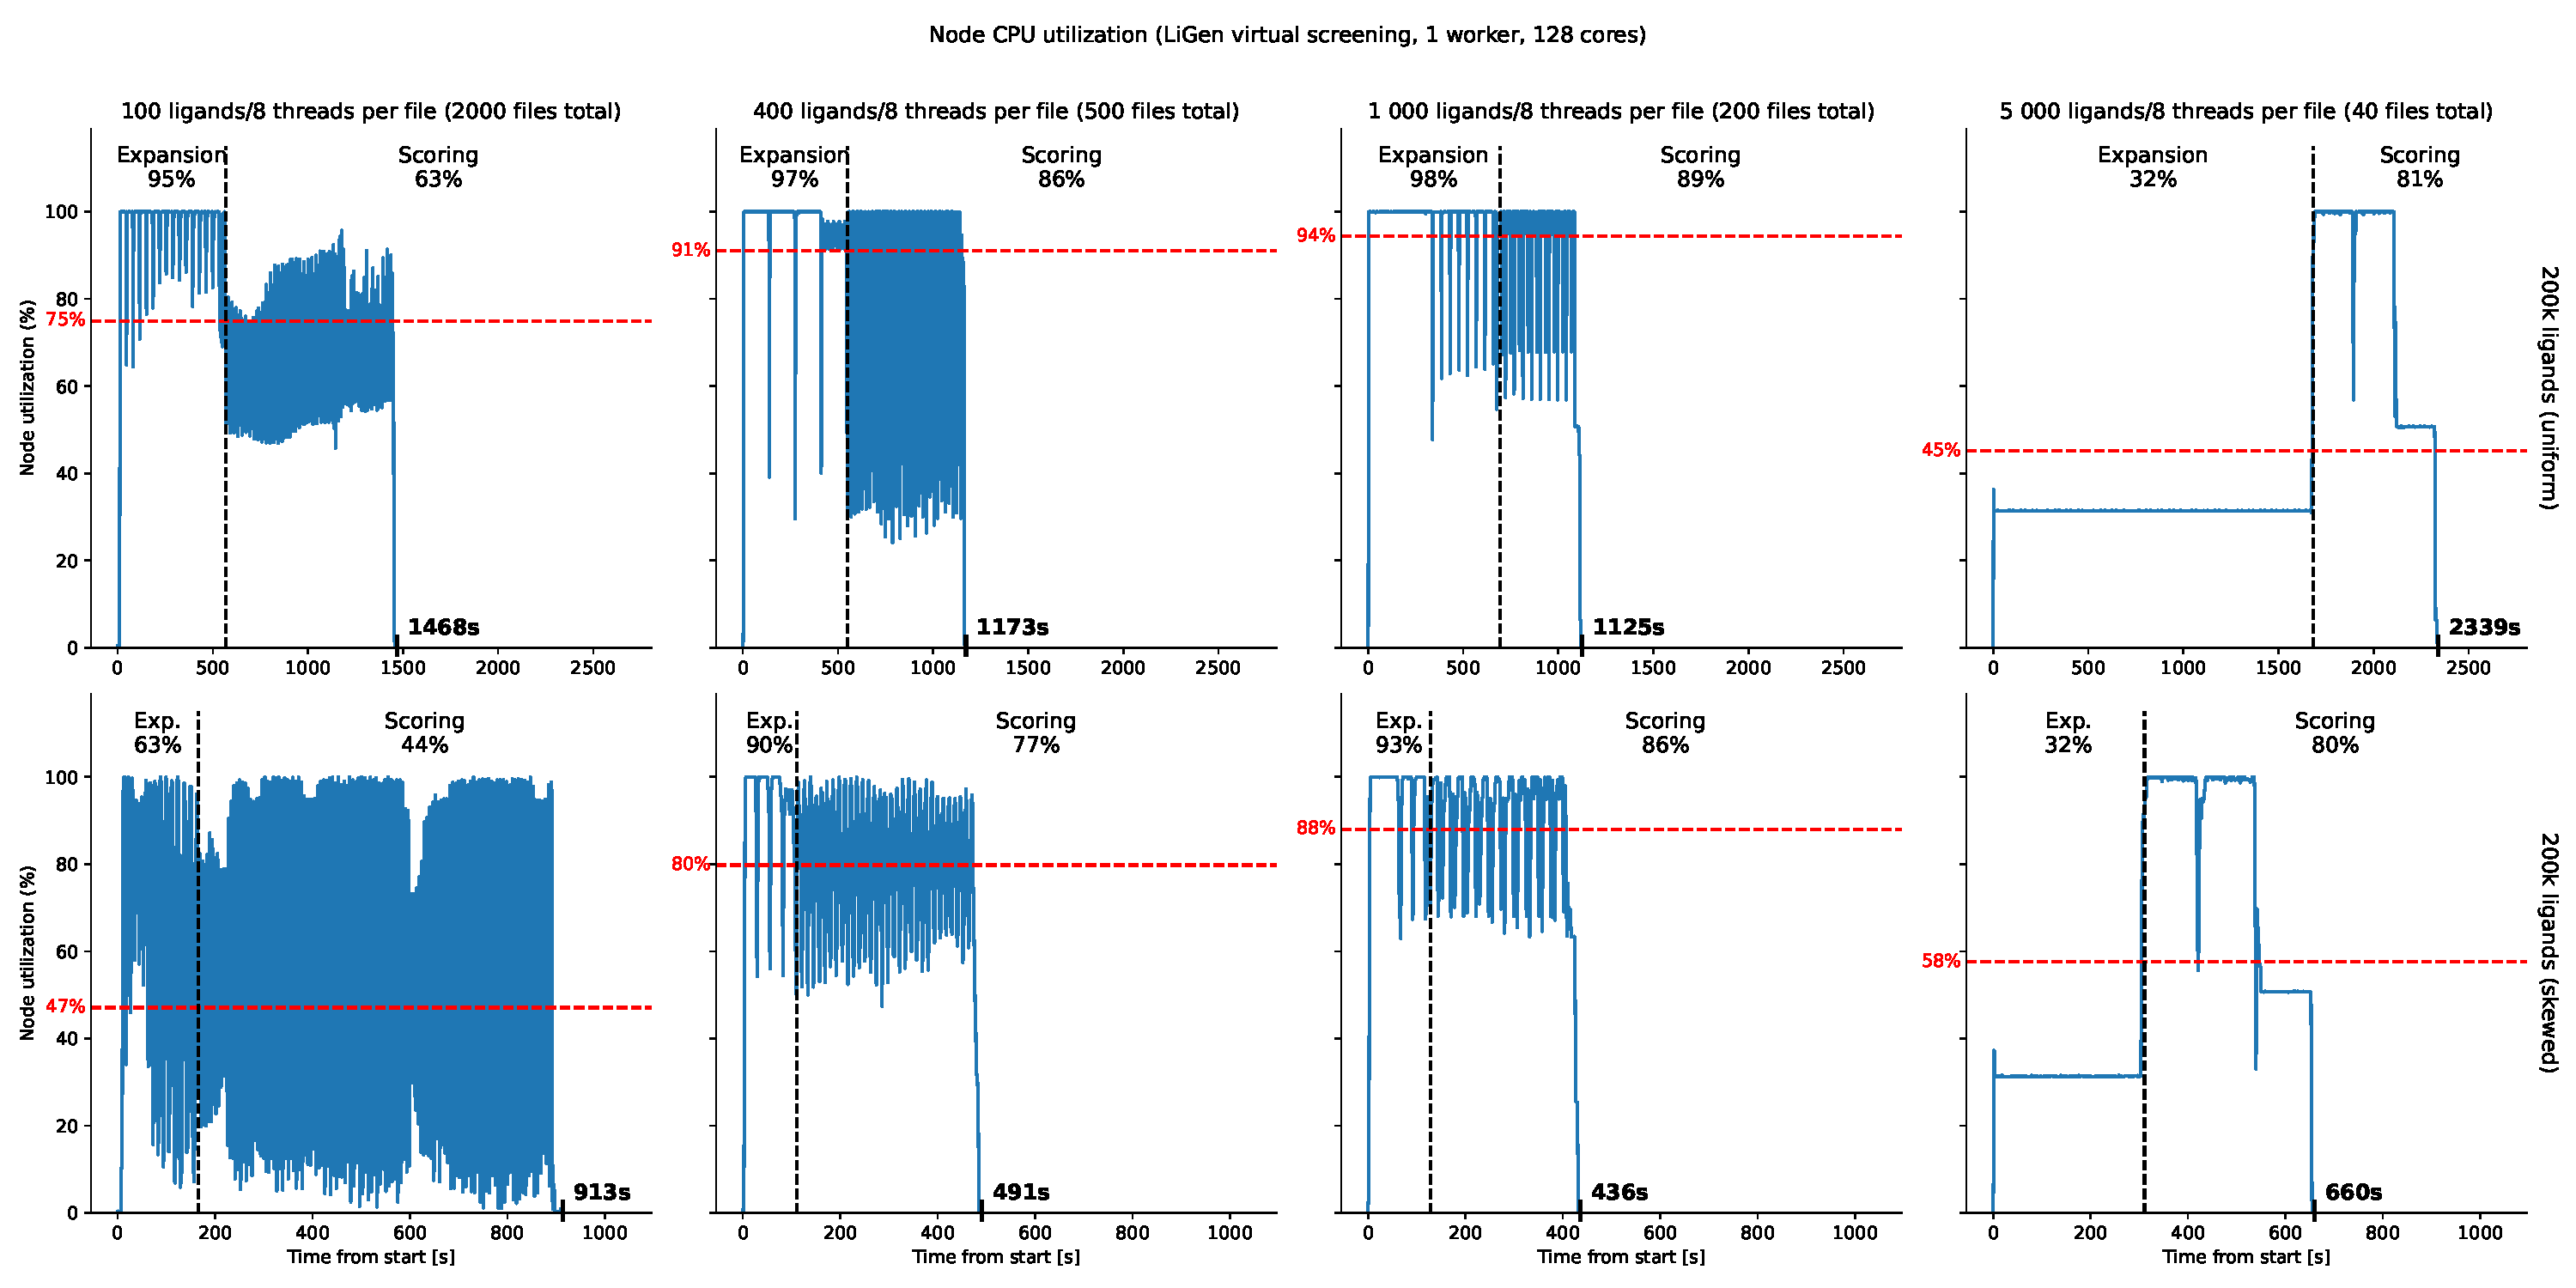
\includegraphics[width=\textwidth]{imgs/hq/charts/ligen-aggregation-utilization}
	\caption{Worker hardware utilization with the LiGen virtual screening workflow}
	\label{fig:hq-ligen-utilization}
\end{figure}

We can see that the parameter affecting the number of ligands per file has a significant effect on
the resulting makespan; using too few or too many ligands results in a longer execution. As
expected, the expansion section needs enough tasks to saturate the available cores, because it is
single-threaded. For $5000$ ligands per file (the rightmost column), the total
number of expansion tasks is only $40$; therefore, the achieved utilization (for
both input files) is only approximately $32\%$, which corresponds to using just
$40$ out of the $128$ available cores. With more than
$128$ files available, the utilization approaches $100\%$ for the
uniform input. For the skewed input file, the utilization for the expansion section is in general
worse than with the uniform input, as expected. With $100$ ligands per file, it
is reduced significantly; unlike with the uniform input, some of the files were expanded much
quicker than others, which led to more load imbalance.

The scoring part is internally parallel and uses all $8$ assigned cores;
therefore, it does not have to be divided into so many tasks. We can see that even with just
$40$ files it achieves approximately $80\%$ utilization for
both input workloads. In fact, with too many files, we can see the overhead associated with the
sequential part of scoring (which needs to be performed for each file separately) starts to
dominate; even with the uniform workload, the \gls{cpu} utilization of the scoring
section with $2000$ files reaches only approximately $63\%$ with
the uniform input and just $44\%$ with the skewed input.

The two configurations in the middle present a sort of a sweet spot; especially with
$1000$ ligands per file, the total average utilization for both workloads is at or
above $88\%$. However, it should be noted that the best configuration will change
based on the number of used workers. This can be observed in~\Autoref{fig:hq-ligen-scalability}, which shows
how does the workflow scale up to $4$ workers ($512$ cores).
The horizontal axis shows the number of workers and the vertical axis shows the duration of the
executed task graph. We can see that with four workers, the configuration with
$400$ ligands per task starts to beat the configuration with
$1000$ ligands per task, simply because the latter configuration is not able to
provide enough parallelism (tasks) to make efficient use of all the available hardware resources.
In general, \hyperqueue{} is able to reduce the makespan with additional workers being
added for all four tested configurations.

\begin{figure}[h]
	\centering
	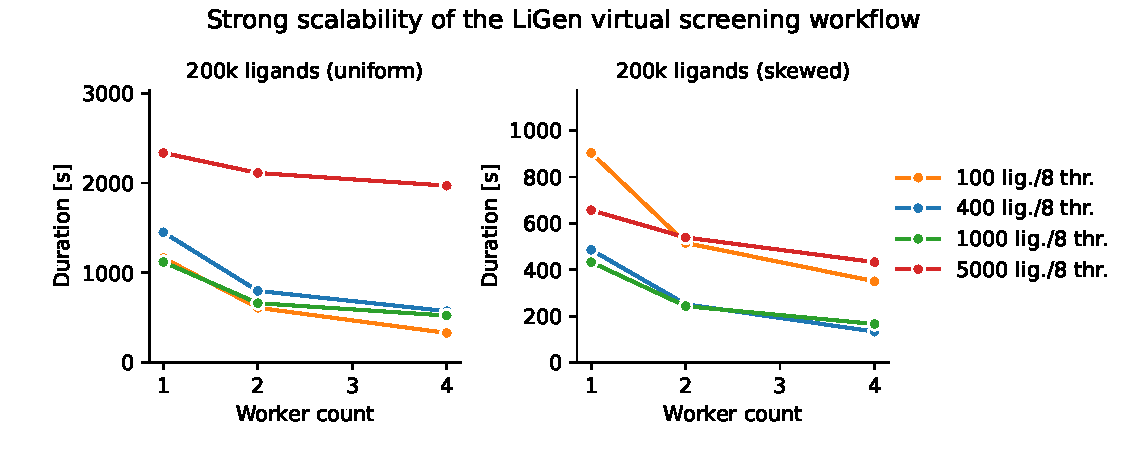
\includegraphics[width=0.8\textwidth]{imgs/hq/charts/ligen-aggregation-scalability}
	\caption{Scalability of the LiGen virtual screening workflow}
	\label{fig:hq-ligen-scalability}
\end{figure}

The results of this experiment have showed that \hyperqueue{} is able to reach high node
utilization even for imbalanced workloads. However, we can also see that even when the overhead of
the task runtime does not get in the way, for some workflows it might be necessary to tune the
number of tasks in order to achieve optimal performance.

\subsection{Automatic allocation}
\label{sec:hq-exp-autoalloc}
This experiment evaluates the ability of the automatic allocator to scale computational resources
both up and down in reaction to computational load. The LiGen virtual screening workflow was
executed using $16$ ligands per file and $8$ threads per
file on an input file containing $24$ thousand ligands with a skewed
distribution of ligands. No workers were explicitly allocated for this experiment; instead, the
automatic allocator was configured to submit allocations that would start a single worker per
allocated node. The maximum number of workers was set to four and the wall-time (the maximum
duration) of the allocations was set to one minute. This very short wall-time was chosen simply to
make the benchmark run shorter and to simulate the situation where an allocation ends in the midst
of a task graph being computed. The experiment was performed with two configurations for the
\emph{idle timeout} duration, which decides after what time a worker (and its allocation) shuts
down when it is fully idle. Each configuration was benchmarked a single time.

\begin{figure}[h]
	\centering
	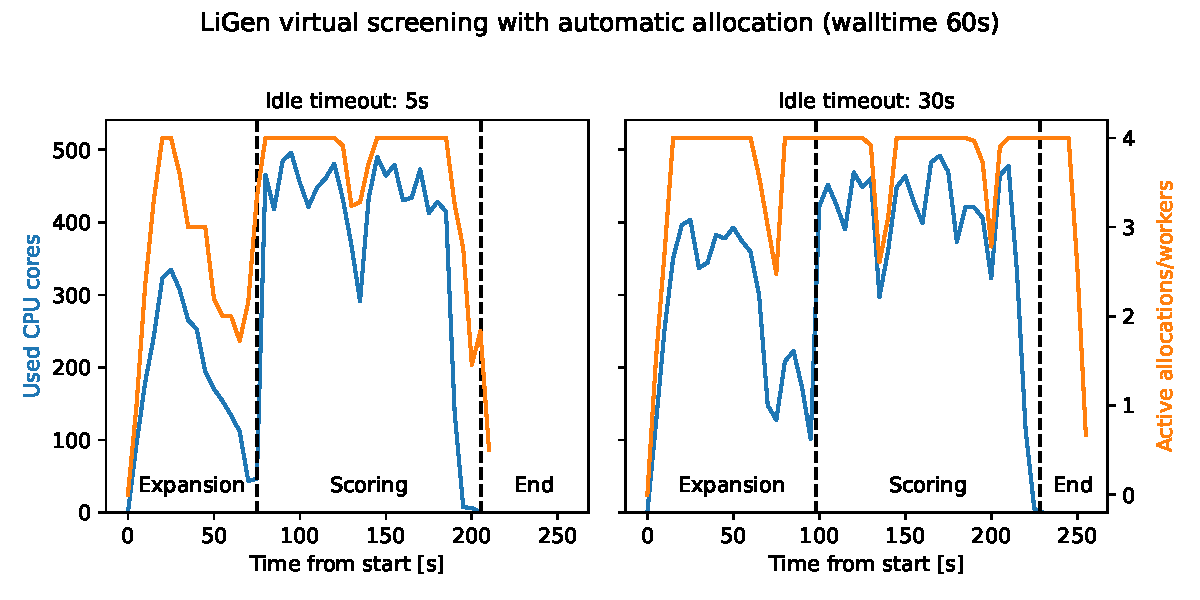
\includegraphics[width=0.8\textwidth]{imgs/hq/charts/ligen-autoalloc-stats}
	\caption{Scaling of allocations using the automatic allocator}
	\label{fig:hq-ligen-autoalloc}
\end{figure}

We can observe the result of the experiment in~\Autoref{fig:hq-ligen-autoalloc}. The horizontal axis shows
the progress of the computation in seconds. The left vertical axis and the blue line shows the
number of cores used for executing tasks (number of running tasks $\times$ cores
required per task). The right vertical axis and the orange line shows the number of active
allocations, which also corresponds to the number of workers, because each allocation spawned
exactly one worker. The dashed vertical lines show individual sections of the computation;
expansion of ligands, scoring of expanded ligands and an \emph{End} section, where the
task graph was already computed and the idle allocations were waiting for the idle timeout to be
applied. Note that when we benchmark automatic allocation, the allocation manager and the global
state of the cluster have a significant influence on the time allocations spend waiting to be
executed in the queue, and thus also on the total makespan of the executed task graph; therefore,
the makespans of these two executions cannot be directly compared.

We can see that allocations were dynamically submitted in response to tasks that needed workers to
execute and that new allocations were quickly created in response to previous allocations ending.
As you may recall, the wall-time was set to only one minute, after which each allocation ended,
which causes the periodic drops in active allocations in both charts. In the left chart, we can see
the results for idle timeout being configured to \SI{5}{\second}. We can observe that in
this case the allocations were scaled down during the expansion part of the workflow, as not that
many resources were required towards the end of expansion. Furthermore, towards the end of the
computation, allocations started being scaled down even before the task graph has finished
computing. In the right chart, where the idle timeout was much longer (\SI{30}{\second}),
the allocations were active for the whole duration of the task graph execution, except for short
periods of time where new allocations had to be spawned due to wall-time being exhausted. All four
allocations were also active up until the very end of the task graph computation, which resulted in
more allocation time being wasted.

With idle timeout \SI{5}{\second}, the workflow has consumed $682$
node-seconds of allocation time, while with idle timeout \SI{30}{\second}, it has consumed
$916$ node-seconds. This shows that it is crucial to configure the idle timeout
properly to avoid wasting allocation time. By default, \hyperqueue{} uses a wall-time of
$1$ hour and an idle timeout of $5$ minutes, which
corresponds to the same wall-time/idle-timeout ratio as the benchmarked configuration with an idle
timeout of \SI{5}{\second}.

\section{Comparison with other task runtimes}
\label{hq:related-work}
Several existing task runtimes and their ability to cope
with challenges that affect task graph execution on \gls{hpc} clusters were described
in~\Autoref{ch:sota}. Even within the particular area of task-based programming that was specified
in~\Autoref{ch:distributed-computing}, there are dozens of tools designed for executing some kind of task
graph, whose features and target use-cases partially overlap with \hyperqueue{}. We will
focus on a smaller subset of task runtimes that enable performing some form of meta-scheduling on
top of allocation managers and can thus be more directly compared with \hyperqueue{}.
Several representatives of these tools will be mentioned in this section.

It should be noted that when comparing task runtimes, we compare not only the inherent properties
of their design and programming model (such as how do they specify dependencies or manage resource
requirements), but also their implementation details (such as what runtime dependencies are
necessary to deploy the task runtime). As was shown in~\Autoref{subsec:estee-schedulers}
and~\Autoref{sec:rsds-dask-overhead-analysis}, implementation details are crucial; they significantly affect both the
efficiency and scalability of the task runtime and they also dictate how easy it is to use and
deploy it. Therefore, we consider it important to compare actual implementations, rather than only
theoretical designs without any implementation available.

% !{\kern1em} - space
% @{} - remove space
%    \begin{tabular}{@{}lc GG !{\kern1em} GGG !{\kern1em} GG@{}}
%    \multicolumn{3}{c|}{\makecell{Task\\interfaces}} &
%    \multicolumn{p{4em}}{c|}{Task\newline{}interfaces} &
% https://stackoverflow.com/questions/1357798/how-to-center-cell-contents-of-a-latex-table-whose-columns-have-fixed-widths

% Inspiration taken from https://tex.stackexchange.com/a/377651/95679
% tasks unrelated to allocations
% map tasks to allocations
% tasks pinned to a specific queue
% task graph partitioning
% load balancing
% generic workers - Parsl no, Merlin no
% auto-allocation
% fault-tolerance - automatic, manual

% Manual task graph partitioning
\newcommand*\manualmap{\LEFTcircle}
% Automatic task graph partitioning
\newcommand*\automaticmap{\CIRCLE}
% Manual fault tolerance
\newcommand*\manualft{\LEFTcircle}
% Automatic fault tolerance
\newcommand*\automaticft{\CIRCLE}

% \begin{noindent}
\begin{table}[h]
%	\aboverulesep=0ex
%	\belowrulesep=0ex
\footnotesize
\newcommand*\rot[1]{\footnotesize\hbox to1em{\hss\rotatebox[origin=br]{-90}{#1}}}
\newcommand*\rotheading[1]{\footnotesize\hbox to1em{\hss\rotatebox[origin=br]{-60}{#1}}}
\newcommand*\feature[1]{\ifcase#1 -\or\LEFTcircle\or\CIRCLE\fi}
\newcommand*\f[3]{\feature#1&\feature#2&\feature#3}
\makeatletter
\newcommand*\ex[9]{#1\tnote{#2}&#3&%
\f#4&\f#5&\f#6&\f#7&\f#8&\f#9&\expandafter\f\@firstofone
}
% Features
\newcommand*\yes{\faThumbsOUp}
%	\newcommand*\no{\faThumbsODown}
\newcommand*\no{-}
\newcommand*\partially{\faThumbsOUp}
% CLI for submitting tasks
\newcommand*\cli{C}
% Workflow files for submitting tasks
\newcommand*\workflowfile{W}
% Python API for submitting tasks
\newcommand*\pythonapi{P}
% Requires Python
\newcommand*\python{Python}
\makeatother
\newcolumntype{A}{c@{}c}
\newcolumntype{B}{c@{}c@{}c}
\newcolumntype{C}{c@{}c@{}c@{}c}
\newcolumntype{D}{c@{}c@{}c@{}c@{}c@{}c@{}c}
\begin{threeparttable}
\begin{tabular}{|l|C|A|A|B|D|A|l|}
\multicolumn{1}{c}{Task runtime} &
\multicolumn{4}{c}{\rotheading{Task interfaces}} &
\multicolumn{2}{c}{\rotheading{Task dependencies}} &
\multicolumn{2}{c}{\rotheading{Fault tolerance}} &
\multicolumn{3}{c}{\rotheading{Meta-scheduling}} &
\multicolumn{7}{c}{Resources} &
\multicolumn{2}{c}{\rotheading{Data transfers}} &
\multicolumn{1}{c}{Deployment}\\
\midrule
& % tool
\rot{CLI} & \rot{Workflow file} & \rot{Python API} & \rot{Dynamic task graphs} & % interfaces
\rot{Explicit} & \rot{Inferred from files} & % dependencies
\rot{Worker failure} & \rot{Server failure} & % fault tolerance
\rot{Graph partitioning} &
\rot{Automatic allocation} & \rot{Generic workers} & % meta-scheduling
\rot{Basic resources} & \rot{Custom resources} & \rot{Non-fungible resources} &
\rot{Related resources} & \rot{Fractional resources} & \rot{Resource variants} &
\rot{Multi-node tasks} & %resources
\rot{Directly between tasks} & \rot{Output streaming} & % data transfers
Runtime dependencies \\ % deployment
\midrule
\gnuparallel{}\hfill\cite{parallel} & \yes & \no & \no & \no & \no & \no & \manualft & \no & \no & \no & \no & \no & \no & \no & \no & \no & \no & \no & \no & \yes & Perl \\
%	\midrule
\hypershell{}\hfill\cite{hypershell} & \yes & \no & \yes & \no & \no & \no & \automaticft & \yes & \manualmap & \yes & \no & \no & \no & \no & \no & \no & \no & \no & \no & \yes & \python \\
%	\midrule
\dask{}\hfill\cite{dask} & \no & \no & \yes & \yes & \yes & \no &
\automaticft & \no & \automaticmap\textsuperscript{\dag} & \yes\textsuperscript{\dag} & \yes & \yes & \yes & \no & \no & \no & \no & \no & \yes & \yes & \python \\
%	\midrule
\ray{}\hfill\cite{ray} & \no & \no & \yes & \yes & \yes & \no & \automaticft & \yes
\textsuperscript{*} & \automaticmap & \no & \yes & \yes & \yes & \no & \yes & \yes & \no & \no & \yes & \partially & \python \\
%	\midrule
\parsl{}\hfill\cite{parsl} & \no & \no & \yes & \yes & \yes & \no & \automaticft &
\no & \automaticmap & \yes & \no & \yes & \no & \no & \no & \no & \no & \yes & \yes & \no & \python \\
%	\midrule
\pycompss{}\hfill\cite{pycompss} & \yes & \no & \yes & \yes & \yes & \no & \automaticft &
\yes\textsuperscript{*} & \manualmap & \no & \no & \yes & \no & \no & \yes\textsuperscript{\dag} & \no & \no & \yes & \yes & \yes & \python, Java \\
%	\midrule
\pegasus{}\hfill\cite{pegasus} & \no & \yes & \yes & \no & \yes & \yes & \automaticft &
\yes & \manualmap & \no & \no & \yes & \no & \no & \no & \no & \no & \no & \no & \yes & \python, Java,
HTCondor~\cite{htcondor} \\
%	\midrule
\balsam{}\hfill\cite{balsam} & \no & \no & \yes & \yes & \yes & \no & \automaticft &
\yes & \automaticmap & \yes & \yes & \yes & \no & \no & \no & \no & \no & \yes & \yes & \no & \python,
PostgreSQL \\
%	\midrule
\autosubmit{}\hfill\cite{autosubmit} & \no & \yes & \no & \no & \yes & \no & \automaticft &
\yes & \manualmap & \yes & \no & \yes & \no & \no & \no & \no & \no & \yes & \no & \no & \python \\
%	\midrule
\fireworks{}\hfill\cite{fireworks} & \no & \yes & \yes & \yes & \yes & \no & \manualft &
\yes & \automaticmap & \yes & \yes & \no & \no & \no & \no & \no & \no & \no & \no & \no & \python, MongoDB \\
%	\midrule
\merlin{}\hfill\cite{merlin} & \no & \yes & \no & \no & \yes & \no & \manualft &
\yes & \automaticmap & \no & \no & \yes & \no & \no & \no & \no & \no & \yes & \no & \no & \python, RabbitMQ/Redis \\
%	\midrule
\snakemake{}\hfill\cite{snakemake} & \no & \yes & \yes & \no & \no & \yes & \automaticft &
\no & \manualmap & \yes\textsuperscript{\dag} & \no & \yes & \yes & \no & \no & \no & \no & \yes & \no & \no & \python \\[2mm]
%	\midrule
\hyperqueue{}\hfill\cite{hyperqueue} & \yes & \yes & \yes & \yes & \yes & \no & \automaticft &
\yes & \automaticmap & \yes & \yes & \yes & \yes & \yes & \yes & \yes & \yes & \yes & \no & \yes & \\
\bottomrule
\end{tabular}
\begin{tablenotes}
\centering
\item \yes{} supported; \no{} not supported; \automaticmap{} automatic; \manualmap{} manual;
\item \textsuperscript{\dag}with an external plugin; \textsuperscript{*}with additional
runtime dependencies
\end{tablenotes}
\caption{Comparison of meta-scheduling task runtimes}
\label{tab:hq-tools-comparison}
\end{threeparttable}
\end{table}
% \end{noindent}

\Autoref{tab:hq-tools-comparison} provides a high-level comparison of \hyperqueue{} and twelve
other task runtimes. It should be noted that there are also many important properties that are not
mentioned in this table; it primarily compares meta-scheduling and resource management aspects
described in this chapter and other features related to challenges described
in~\Autoref{ch:sota}. Furthermore, there is no single universally best task runtime; each one
has a different programming model and a different set of features and trade-offs based on which
use-cases it was primarily designed for. A brief description of each compared task runtime can
be found in~\Autoref{app:task-runtime-descriptions}.

The first section of the table, \emph{Task interfaces}, shows which interfaces can be used to
submit tasks and if they support modifying task graphs dynamically. \glsxtrshort{cli}
specifies that tasks can be submitted from the command-line, \emph{Workflow file} specifies that
task graphs can be defined using e.g.\ \gls{yaml} or \gls{toml} files and
\emph{Python \glsxtrshort{api}} marks runtimes that provide the option to specify tasks using Python. Note
that the \gls{cli} column indicates that tasks and task graphs can be actually
defined and submitted using the command-line without requiring additional input files, not just
that the runtime provides some form of a \gls{cli} (which is offered by most runtimes). The last column,
\emph{Dynamic task graphs}, states whether the task runtime supports adding new tasks to already
submitted task graphs dynamically, which is useful e.g.\ for expressing iterative workflows.

Most evaluated task runtimes provide a Python \gls{api}, as it enables the most
general way of defining task graphs. However, it is relatively rare for other tools to offer a
comprehensive \gls{cli} that could be used to submit simple task graphs without the
need to implement a script using (an imperative) programming language. \merlin{} and
\autosubmit{} only allow defining task graphs using workflow files, which can also be
quite verbose for simple use-cases. \hyperqueue{} offers both a terminal interface for
simple use-cases, a Python \gls{api} for more complex task graphs and it also
supports workflow files.

The second section, \emph{Task dependencies}, marks the ability to express dependencies between
tasks. \emph{Explicit} dependencies are described by the user in the task graph definition,
usually by mentioning a set of task identifiers on which a given task depends.
\gnuparallel{} and \hypershell{} do not allow specifying task dependencies, as
they are designed mostly for scenarios where users simply need to execute a large number of tasks
in parallel. Most other tools allow expressing dependencies between tasks explicitly.
\pegasus{} and \snakemake{} are also able to infer dependencies
automatically based on input/output files consumed/produced by the individual tasks. For
\snakemake{}, it is the only way to express dependencies, which can limit performance
for task graphs with many tasks, as every dependency necessitates the creation of a file on a
filesystem.

The third section, \emph{Fault tolerance}, describes what happens after a worker or a server
failure. Task runtimes that can automatically restart tasks after a worker failure are marked with
\automaticft; those that require user action to recompute failed tasks are marked with \manualft.
All the evaluated task runtimes provide support for at least some kind of resilience against worker
failures; it is a truly fundamental feature without which it would be infeasible to execute task
graphs. To be resilient against server failures, the task runtime should be able to restore the
state of already computed tasks and all already submitted task graphs when the main server or
scheduler component crashes (e.g.\ when it is executed on a login node that abruptly shuts down).
This property is useful for avoiding unnecessary re-execution of long-running task graphs.
Resilience against server failures is not supported so ubiquitously, although is is still a
relatively common feature. However, most task runtimes require an external service or a database
instance to implement server persistence, which can complicate their deployment.

The fourth section, \emph{Meta-scheduling}, specifies three properties related to executing tasks
on top of allocations. The following list describes the individual columns:

\begin{description}[wide=0pt,itemsep=0pt,topsep=4pt]
	\item[Graph partitioning] states whether the task runtime can assign tasks to allocations fully automatically (\automaticmap)
		or if users have to partition tasks manually (\manualmap). As already mentioned
		in~\Autoref{challenge:allocation-manager}, tools such as \pegasus{}, \autosubmit{} or
		\snakemake{} require users to manually specify how should tasks be grouped into
		allocations, which requires more work from the user and it can also limit the achieved hardware
		utilization. Other task runtimes, such as \dask{} or \balsam{}, are
		able to fully automatically assign tasks to allocations without any intervention from the user,
		same as \hyperqueue{} does.

	\item[Automatic allocation] highlights task runtimes that are able to automatically submit \emph{\gls{hpc} allocations}. There are
		various levels of support for this feature. \snakemake{} or \autosubmit{}
		simply submit allocations that are designed for executing a specific task (or a group of tasks),
		while other task runtimes, such as \dask{}, \balsam{} or
		\hyperqueue{}, submit allocations dynamically based on the current computational load and
		task state; these allocations then start a generic worker that is not tied to any specific task or
		a subset of tasks. Unlike \hyperqueue{}, \dask{} and
		\balsam{} support configuring only a single allocation manager queue into which new
		allocations can be submitted.

	\item[Generic workers] states whether the task runtime supports provisioning generic workers that can execute any tasks
		whose resource requirements are compatible with it, without requiring users to preconfigure workers
		statically for a specific subset of tasks (which makes load balancing less flexible).
		\merlin{} requires preconfiguring queues that are used for executing specific tasks
		(such as a task that requires exactly two nodes or sixteen \gls{cpu} cores to
		execute). A similar approach is used by \parsl{}. On the other hand,
		\dask{} or \hyperqueue{} make worker spawning very easy by using a single
		generic command, since their workers are not tied to any specific subset of tasks.
\end{description}

The following section, \emph{Resources}, deals with resource management. It shows which task
runtimes are only able to specify basic (such as \gls{cpu}, \gls{gpu}
or memory) task resource requirements and which are able to define custom resource kinds. Support
for custom resource requirements (and thus heterogeneous clusters) is not very common; apart from
\hyperqueue{}, only \dask{}, \ray{} and
\snakemake{} allow users to define their own resource kinds that are then used during
task scheduling. The following four columns describe the support for the complex heterogeneous
resource management concepts that were described in~\Autoref{sec:heterogeneous-resources}. As was already noted,
support for these features is not prevalent in existing task runtimes. One notable exception is
\ray{}, which supports both related resources and fractional resources.

The \emph{Multi-node} column then shows which programming models enable describing multi-node
tasks. Note that the table only considers this feature as being supported in task runtimes that
provide the ability to assign the number of nodes \emph{per task}, not just per task graph
or per allocation. We can see that \snakemake{} is the only task runtime apart from
\hyperqueue{} that supports both custom resource kinds and multi-node tasks.

The penultimate section, \emph{Data transfers}, states whether it is possible to exchange data
outputs between tasks directly over the network without going through the filesystem
(\emph{Directly between tasks}) and if the task runtime offers the ability to stream standard (error)
output of tasks over the network to overcome distributed filesystem limitations
(\emph{Output streaming}). Direct data transfer of task outputs is supported by several
Python-first task runtimes, such as \dask{} or \ray{}; however, it
is not supported by \hyperqueue{}.

The last section, \emph{Deployment}, specifies which runtime dependencies and external
services have to be available in order to execute the task runtime. We can see that almost all
evaluated task runtimes require a Python interpreter, as it is a very popular technology for
working with tasks. Some task runtimes, such as \merlin{} or \fireworks{},
additionally require an external service for managing persistence or task assignments; these can be
challenging to deploy on \gls{hpc} clusters. Note that this column specifies the
\emph{required} runtime dependencies, which are necessary for the task runtime to function.
It does not mention optional dependencies; for example, \hyperqueue{}'s Python
\gls{api} of course also requires a Python interpreter, but \hyperqueue{}
itself can operate without it.

Even though several existing task runtimes also leverage meta-scheduling, they do not offer a
holistic set of features that would help resolve the most pressing issues of task graph execution
on heterogeneous supercomputers all at once. Some of them are not focused primarily on
\gls{hpc} problems, while others tie tasks to allocations too strongly, which reduces
load-balancing opportunities and limits local prototyping. Most task runtimes also require runtime
dependencies that might complicate their deployment.

\hyperqueue{} treats \gls{hpc} as a first-class citizen and provides a
unified set of features that help task graph authors execute their task graphs in an easy way on
\gls{hpc} clusters. It is also very efficient and can scale to a large number of
hardware resources while being trivial to deploy. Furthermore, \hyperqueue{} provides
unique resource scheduling features in the form of non-fungible resources, related resources,
fractional resource requirements and resource variants, which can help improve the achieved
hardware utilization on heterogeneous clusters. On the other hand, in the current version, its
programming model does not yet integrate direct data transfers between tasks,which can be limiting
for use-cases that require this functionality.

\section*{Summary}
This chapter has presented a meta-scheduling and resource management design for executing task
graphs on heterogeneous \gls{hpc} clusters that was created in order to overcome the
issues mentioned in~\Autoref{ch:sota}. It has also introduced \hyperqueue{}, a
distributed task runtime that implements this design through an \gls{hpc} focused
programming model, which enables ergonomic execution of workflows on supercomputers. It is able to
meta-schedule tasks to provide load balancing among separate allocations while respecting complex
resource requirements that can be arbitrarily configured separately for each task. Its automatic
allocator can submit allocations fully autonomously on behalf of the user, which further simplifies
the execution of \hyperqueue{} task graphs. It also offers both a straightforward
\gls{cli} and a Python \gls{api} for more complex use-cases and it is
also trivial to deploy on supercomputers.

The overhead and scalability of \hyperqueue{} was evaluated in various situations. The
results indicate that it consumes little resources, introduces a reasonable amount of overhead and
can scale to tens of nodes and thousands of cores. The experiments have also shown that it is more
than competitive against \dask{}, a very popular task runtime that is being
commonly used for running task graphs on distributed clusters.

Several ideas for the future improvement of \hyperqueue{} will be summarized in the final
chapter.


	\chapter{Conclusion}
	\label{ch:conclusion}
	The main goals of this thesis were to describe and analyze existing challenges of task graph
execution on \gls{hpc} systems, with the main focus on efficiency and usage
ergonomics, and design and implement approaches for alleviating them. The main issues affecting
\gls{hpc} task graph execution were described in~\Autoref{ch:sota}, which
has identified several areas that can cause problems when executing task graphs on modern
heterogeneous \gls{hpc} clusters, and outlined motivation for work presented in
the rest of the thesis.

The following two chapters focused on the performance and efficiency aspects of executing task
graphs.~\Autoref{ch:estee} has introduced \estee{}, a simulation
environment designed for prototyping task schedulers and benchmarking various aspects of task graph
execution. We have used \estee{} to perform a comprehensive study of several task
scheduling algorithms and examine several hypotheses of the effect of various factors on the
performance of the scheduler. Through our experiments, we have found that the
\emph{b-level} heuristic combined with work-stealing provides a solid baseline
scheduling algorithm that achieves good performance across various kinds of task graphs. This
scheduling approach was then used for implementing efficient scheduling in
the~\rsds{} and~\hyperqueue{} task runtimes. Our results have also
indicated that while important, task scheduling might not be the most crucial factor that affects
the performance of task graph execution in certain scenarios, and that even a completely random
scheduler might be competitive.

\Autoref{ch:rsds} focused on the performance bottlenecks of a real-world task runtime
\dask{} in a non-simulated
environment, to leverage our insights gained from the previous scheduler experiments. Our analysis
has shown that \dask{} is severely limited by its implementation
characteristics, moreso than its scheduler. In particular, it is limited by its choice of Python as
an implementation language, which can introduce massive overhead particularly for
\gls{hpc} use-cases. We have proposed and implemented~\rsds{},
a backwards-compatible implementation of the \dask{} server written in Rust,
which was carefully designed to minimize runtime overhead. Our experiments demonstrated that such
an optimized server implementation can improve the scalability and end-to-end performance of
\dask{} workflows by several times, even though it uses a simpler scheduling
algorithm.

\Autoref{ch:hyperqueue} combined the gained performance insights with a focus on
the ergonomic aspects of designing and executing task graphs on supercomputers. It introduced a
general meta-scheduling approach designed primarily to avoid complications caused by the need to
interact with \gls{hpc} allocation managers and also to support the complex nature
of modern heterogeneous clusters. The described method completely separates task submission from
computational resource provisioning, which enables fully dynamic and automatic load balancing even
across different allocations. It is combined with a resource management system that allows tasks to
express complex resource requirements in a generic way, while still making it trivial to provision
computational resources.

The described approach has been implemented in \hyperqueue{}, an
\gls{hpc}-optimized task runtime that was designed to make it simple to execute
task graphs in the presence of allocation managers. The most important features of
\hyperqueue{} have been described in this chapter, such as its support for complex
resource management and multi-node tasks, fault-tolerant task execution and automatic submission of
allocations. The overhead and scalability of this task runtime were also evaluated on several
benchmarks designed to push it to its performance limits. The results of these experiments indicate
that it does not introduce significant overhead and can be used to efficiently scale task graphs to
a large amount of computational resources.

\hyperqueue{} is a culmination of the work described in this thesis; it was
designed as a unified solution for removing bottlenecks and challenges from task graph execution on
supercomputers. The following list describes how \hyperqueue{} deals with challenges
introduced by~\Autoref{ch:sota}, and also which improvements could be made to it as future
work to further improve its ability to provide ergonomic and efficient task graph execution on
\gls{hpc} clusters.
\begin{description}[wide=0pt]
	\item[Interaction with allocation manager] The used meta-scheduling approach removes the need for the workflow author to think about mapping
		tasks to allocations or dealing with various allocation limits. And thanks to the automatic
		allocator, users do not even need to submit any allocations by themselves. The automatic allocator
		could be extended with task duration or allocation start time predictions in the future, to improve
		its decisions on when to actually submit allocations.
	\item[Cluster heterogeneity] \hyperqueue{} provides comprehensive support for heterogeneous
		clusters by enabling tasks to specify arbitrary resource requirements, and by matching these
		requirements with resources provided by workers. In addition to basic resources, support for
		\gls{numa}, \gls{gpu} core pinning and time requests, it also
		supports complex resource requirements in the form of resource variants and fractional resources,
		which can deal with the most complex resource management scenarios. Workers also provide automatic
		detection of available resources, which further improves the ergonomics of running workflows with
		heterogeneous clusters.
	\item[Data transfers] \hyperqueue{} does not currently support direct data transfers
		between tasks, i.e.\ enabling tasks to pass their outputs as inputs to dependent tasks through
		network communication. This limits its applicability (or at least its ergonomics) in scenarios that
		need to exchange large amounts of outputs between tasks. Implementing data transfers would expand
		the set of workflows that can be naturally executed with it, and it could also improve performance
		by avoiding filesystem \gls{io}.

		For use-cases that are limited by \gls{io} bandwidth due to creating too many
		standard (error) output files on distributed filesystems, \hyperqueue{} offers
		\emph{output streaming}, which is able to avoid filesystem limitations by streaming task output
		to the server and storing it in a single file.
	\item[Fault tolerance] \hyperqueue{} offers fault tolerance by default; tasks that do not
		finish computing successfully due to reasons outside their control are automatically rescheduled to
		a different worker, without requiring any manual user intervention. Workers are designed to be
		ephemeral; because they are usually executed in relatively short-running allocations, their
		failures are thus handled gracefully. The server itself is also fault-tolerant and can reload its
		task database after being restarted.
	\item[Multi-node tasks] \hyperqueue{} provides built-in support for multi-node tasks, and
		can even combine them with standard single-node tasks within the same task graph. It also provides
		basic integration with common multi-node technologies like \gls{mpi} to make their
		usage in multi-node tasks easier. Multi-node tasks could be further extended to be more granular,
		so that a multi-node task would not necessarily require its whole node for execution, and for some
		use-cases it would also be very useful to have the ability to combine multi-node tasks with data
		transfers.
	\item[Scalability] Experiments presented in~\Autoref{hq:evaluation} demonstrate that \hyperqueue{} is
		able to scale to \gls{hpc}-level workflows and that it does not introduce
		significant overhead over executing tasks manually. Its performance could be further improved by
		integrating \gls{hpc}-specific technologies, such as
		InfiniBand~\cite{infiniband} or \gls{mpi}, to speed-up network
		communication or filesystem \gls{io}, or by adding support for stateful task
		environments. These could help avoid the need to create a separate Linux process for each executed
		task, which can have a non-trivial overhead on certain \gls{hpc} clusters, as was
		demonstrated by our experiments.
	\item[Iterative computation] While it is possible to express task graphs that need to be created in a dynamic fashion or that
		leverage iterative computation using the Python \gls{api}, it is currently not
		fully ergonomic for the users, as separate \hq{} jobs need to be submitted in
		this case. As a future extension, \hyperqueue{} could allow adding tasks to existing
		jobs fully dynamically, which would make it much simpler to express use-cases where the structure
		of the task graph is not fully known before its execution starts.
	\item[Deployment] In terms of ease-of-deployment, \hyperqueue{} is essentially optimal; it is
		distributed as a single binary that runs fully in user-space and that does not have any
		dependencies. Its users thus do not have to install any libraries or deploy complex services on the
		target supercomputer (which can be very difficult or even impossible in some cases) in order to use
		it. It is also simple to make it completely self-contained by statically linking a
		\emph{C} standard library into it, which would remove its only runtime dependency
		on the \texttt{glibc} standard library implementation. Its Python
		\gls{api}, which is an optional component, is distributed as a standard Python
		package that can be easily installed using standard Python package management tools, on a variety
		of Python versions.
\end{description}

To summarize, this thesis makes the following contributions:
\begin{itemize}
	\item It introduces a task graph simulator for evaluating the quality of task schedulers under various
	      conditions and provides an extensive evaluation of several scheduling algorithms using this
	      simulator.
	\item It provides an analysis of the performance bottlenecks of a state-of-the-art task runtime
	      \dask{} and introduces an alternative implementation of its server that provides
	      significant performance improvements in \gls{hpc} scenarios while retaining
	      backwards compatibility.
	\item Primarily, it proposes an approach for effortless execution of task graphs in the presence of
	      \gls{hpc} allocation managers and provides an implementation of this approach in
	      the \hyperqueue{} task runtime.
\end{itemize}

\section{Impact}
This final section summarizes the impact that \rsds{} and
\hyperqueue{} had on several real-world projects.

\subsection*{\rsds{}}
After we had an indication that \rsds{} could be leveraged to improve the
efficiency of existing \dask{} workflows, we contacted the authors and
maintainers of \dask{} and presented them our research and
\rsds{}. Although replacing their server implementation or switching from Python
to a different implementation language was not a feasible approach for them, some of the ideas
implemented in \rsds{} have since been adapted in the \dask{}
project. This helped alleviate some of the bottlenecks that we have discovered with our
experiments, and improved the performance of \dask{} in
general\footnoteurl{https://github.com/dask/distributed/issues/3139}\footnoteurl{https://github.com/dask/distributed/issues/3783}\footnoteurl{https://github.com/dask/distributed/issues/3872}.

\subsection*{\hyperqueue{}}
\hyperqueue{} has already been adopted in several projects, and it is also being
actively used by various researchers and teams across several European \gls{hpc}
centers. It has been proposed as one of the designated ways for executing
\gls{hpc} computations in several supercomputing centers and clusters, such as
LUMI~\cite{it4i-lumi}, CSC-FI~\cite{puhti-hq,puhti-hq-2},
IT4Innovations~\cite{it4i-hq} or CINECA~\cite{cineca}.

In addition to being used directly by \gls{hpc} users and scientists,
\hyperqueue{} can also be integrated as a general task execution system into other
tools, thanks to its sophisticated resource management and task scheduling capabilities. This has
been leveraged by several workflow management systems that have integrated
\hyperqueue{} as one of their task execution backends, such as
Aiida~\cite{aiida-hq}, NextFlow~\cite{nextflow-hq},
UM-Bridge~\cite{umbridge}, StreamFlow~\cite{streamflow-hq},
ERT~\cite{ert} or HEAppE~\cite{heappe}.

\hyperqueue{} is also used in various research projects. As an example,
scientists from the Czech Academy of Sciences use it to execute simulations that analyze data from
the ATLAS~\cite{atlas} experiment performed at CERN. Thanks to
\hyperqueue{}, they were able to improve the achieved hardware utilization on the
IT4Innovations Karolina~\cite{karolina} supercomputer by 30\%, which saves them tens of
hundreds of node hours per year~\cite{cern-hq}. \hyperqueue{} has also
been used to execute workflows in several projects funded by the European Union, such as
EVEREST~\cite{everest}, ACROSS~\cite{across},
EXA4MIND~\cite{exa4mind} and MaX~\cite{max}. It was especially useful
for the LIGATE~\cite{ligate} project, where it was used to implement several
\gls{md} workflows that were executed using hundreds of thousands of
\gls{cpu} and \gls{gpu} hours on the most powerful European
supercomputers.

Given the use-cases mentioned above, I believe that the practical applicability of the proposed
task graph execution design has been demonstrated, and that this thesis has thus achieved the goals
that it originally set out to. I am confident that \hyperqueue{} provides a tangible
benefit in terms of ergonomic and efficient execution of task graphs on supercomputers, and that it
resolves many of the challenges that have been described extensively in this thesis through its
\gls{hpc}-driven design. I hope that \hyperqueue{} will eventually
see even more widespread usage in the \gls{hpc} community.

\end{spacing}

\begin{spacing}{1}
	\chapter*{List of own publication activities}
	\label{ch:listofstudentsownpublicationactivities}
	\addcontentsline{toc}{chapter}{\nameref{ch:listofstudentsownpublicationactivities}}

	All citation data presented below is actual as of August 2024, unless otherwise
specified. Citation data was taken from Scopus\footnoteurl{https://www.scopus.com}.
Self-citation is defined as a citation with a non-empty intersection between the authors of the citing and the cited paper.
SJR (Scientific Journal Rankings) ranking was taken from Scimago Journal\footnoteurl{https://www.scimagojr.com},
IF (Impact Factor) ranking was taken from Oxford Academic\footnoteurl{https://academic.oup.com/bioinformatics}.
The h-index of the author of this thesis according to the Scopus database is \texttt{5},
with \texttt{79} total citations (both excluding self-citations).

Note that Ada Böhm was named Stanislav Böhm in older publications.

\begin{refsection}
\renewcommand*{\mkbibnamegiven}[1]{%
	\ifitemannotation{highlight}
	{\textbf{#1}}
	{#1}}

\renewcommand*{\mkbibnamefamily}[1]{%
	\ifitemannotation{highlight}
	{\textbf{#1}}
	{#1}}

\section*{Publications Related to Thesis}
	\begin{itemize}
		\item\fullcite{hyperqueue}\par{}Total citations: 0, venue: journal (SJR 0.544)
		\item\fullcite{rsds}\par{}Total citations: 7 (2 self-citations), venue: conference proceedings
		\item\fullcite{estee}\par{}Total citations: 1 (no self-citations), venue: journal (SJR 0.684)
		\item\fullcite{ligate}\par{}Total citations: 4 (4 self-citations), venue: conference proceedings
	\end{itemize}

	\subsection*{Posters}
	\begin{itemize}
		\item\fullcite{hyperqueue_poster}\par{}Presented at the SuperComputing'21 conference.
		\item\fullcite{hyperqueue2_poster}\par{}Presented at the HPCSE (High Performance
		Computing in Science and Engineering) 2022 conference.
		\item\fullcite{estee_poster}\par{}Presented at the SuperComputing'19 conference.
	\end{itemize}

\section*{Publications Not Related to Thesis}
	\begin{itemize}
		\item\fullcite{sisa}\par{}Total citations: 44 (20 self-citations), venue: conference proceedings
		\item\fullcite{graphminesuite}\par{}Total citations: 10 (7 self-citations), venue: journal (SJR 2.376)
		\item\fullcite{spin}\par{}Total citations: 10 (3 self-citations), venue: conference proceedings
		\item\fullcite{spin2}\par{}Total citations: 19 (4 self-citations), venue: conference proceedings
		\item\fullcite{smi}\par{}Total citations: 26 (2 self-citations), venue: conference proceedings
		\item\fullcite{haydi}\par{}Total citations: 0, venue: conference proceedings
		\item\fullcite{pycaverdock}\par{}Total citations: 0, venue: journal (IF 5.8)
		\item\fullcite{traffic_simulator_1}\par{}Total citations: 4 (4 self-citations), venue: conference proceedings
		\item\fullcite{traffic_simulator_2}\par{}Total citations: 1 (1 self-citation), venue: conference proceedings
	\end{itemize}
\end{refsection}


	%	\chapter*{List of projects}
	%	\label{ch:listofprojects}~\addcontentsline{toc}{chapter}{\nameref{ch:listofprojects}}
	%	% TODO(Honza): ask what to write here
During my doctoral studies, I have participated in the following projects:
%\end{itemize}%    \end{enumerate}%        \item ACROSS%        \item LIGATE%        \item EVEREST%        \item ANTAREX%    \begin{enumerate}%\begin{itemize}

% SGS - SP2018/142 - Optimization of machine learning algorithms for \gls{hpc} platform II
% SGS - SP2019/108 - Extension of \gls{hpc} platforms for executing scientific pipelines
% SGC - SP2020/167 - Extension of \gls{hpc} platforms for executing scientific pipelines 2
% Národní program udrženosti II (NPU II) č. LQ1602
% PERMED (Technologická agentura ČR, projekt č. TN01000013)
% Ullmanna HS
% Antarex
% - This work has been partially funded/was supported by ANTAREX, a project supported by the EU H2020 FET-\gls{hpc} program under grant agreement No. 671623.
% Exaqute
% - This work was supported by the ExaQUte project - the European Union’s Horizon 2020 research and innovation programme under grant agreement No. 800898.
% Everest (EU Horizon 2020, grant č. 957269)
% - This work was supported by the EVEREST project - the European Union’s Horizon 2020 research and innovation programme under grant agreement No. 957269.
% Ligate (EU Horizon 2020, grant č. 956137)
% - This work was supported by the LIGATE project. This project has received funding from the European High- Performance Computing Joint Undertaking (JU) under grant agreement No 956137. The JU receives support from the European Union’s Horizon 2020 research and innovation programme and Italy, Sweden, Austria, the Czech Republic, Switzerland. This project has received funding from the Ministry of Education, Youth and Sports of the Czech Republic (ID: MC2102).
% Across
% - This work was supported by the ACROSS project. This project has received funding from the European High- Performance Computing Joint Undertaking (JU) under grant agreement No 955648. The JU receives support from the European Union’s Horizon 2020 research and innovation programme and Italy, France, the Czech Republic, the United Kingdom, Greece, the Netherlands, Germany, Norway. This project has received funding from the Ministry of Education, Youth and Sports of the Czech Republic (ID: MC2104).


	% Bibliography
	\renewcommand*{\bibfont}{\small}
	\printbibliography[heading=bibintoc, title={Bibliography}]
\end{spacing}

\appendix
\chapter{\estee{} benchmark definitions}
\begin{figure}[h]
    \centering
    \begin{subfigure}{.2\textwidth}
        \centering
        
\includegraphics[width=.8\textwidth]{imgs/estee/shapes/plain}
        \caption{}
        \label{fig:tg-plain}
    \end{subfigure}%
    \begin{subfigure}{.2\textwidth}
        \centering
        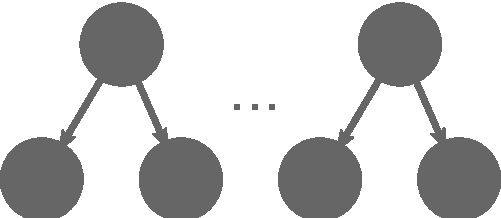
\includegraphics[width=.8\linewidth]{imgs/estee/shapes/fork}
        \caption{}
        \label{fig:tg-fork}
    \end{subfigure}
    \begin{subfigure}{.2\textwidth}
        \centering
        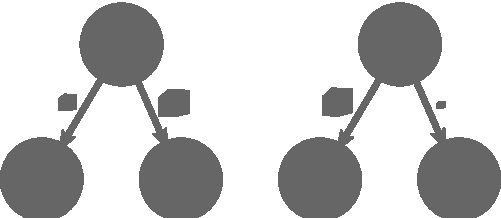
\includegraphics[width=.8\linewidth]{imgs/estee/shapes/fork2}
        \caption{}
        \label{fig:tg-fork2}
    \end{subfigure}
    \begin{subfigure}{.2\textwidth}
        \centering
        \includegraphics[width=.8\linewidth]{imgs/estee/shapes/v}
        \caption{}
        \label{fig:tg-v}
    \end{subfigure}
    \\
    \begin{subfigure}{.2\textwidth}
        \centering
        \includegraphics[width=.8\linewidth]{imgs/estee/shapes/w}
        \caption{}
        \label{fig:tg-w}
    \end{subfigure}
    \begin{subfigure}{.2\textwidth}
        \centering
        \includegraphics[width=.8\linewidth]{imgs/estee/shapes/merge}
        \caption{}
        \label{fig:tg-merge}
    \end{subfigure}
    \begin{subfigure}{.2\textwidth}
        \centering
        \includegraphics[width=.8\linewidth]{imgs/estee/shapes/merge-triplets}
        \caption{}
        \label{fig:tg-merge-triplets}
    \end{subfigure}
    \begin{subfigure}{.2\textwidth}
        \centering
        \includegraphics[width=.8\linewidth]{imgs/estee/shapes/triplets}
        \caption{}
        \label{fig:tg-triplets}
    \end{subfigure}
    \\
    \begin{subfigure}{.2\textwidth}
        \centering
        \includegraphics[width=.8\linewidth]{imgs/estee/shapes/grid}
        \caption{}
        \label{fig:tg-grid}
    \end{subfigure}
    \begin{subfigure}{.2\textwidth}
        \centering
        \includegraphics[width=.8\linewidth]{imgs/estee/shapes/splitters}
        \caption{}
        \label{fig:tg-splitters}
    \end{subfigure}
    \begin{subfigure}{.2\textwidth}
        \centering
        \includegraphics[width=.8\linewidth]{imgs/estee/shapes/conflux}
        \caption{}
        \label{fig:tg-conflux}
    \end{subfigure}
    \begin{subfigure}{.2\textwidth}
        \centering
        \includegraphics[width=.8\linewidth]{imgs/estee/shapes/fern}
        \caption{}
        \label{fig:tg-fern}
    \end{subfigure}

    \caption{Task graph shapes in the \emph{elementary} \estee{} benchmark data set}
    \label{fig:estee-elementary-shapes}
\end{figure}

\begin{table}[h]
    \centering
    \begin{tabular}{l|lrrrr|T}
        \toprule
        Graph            & D & \#T & \#O   & TS     & LP  & \normalsize{Description}     \\
        \midrule
        plain1n          & e & 380 & 0     & 0.00   & 1   & Independent tasks;
        normally distributed durations (Fig.~\ref{fig:tg-plain})                         \\
        plain1e          & e & 380 & 0     & 0.00   & 1   & Independent tasks;
        exponentially distributed durations (Fig.~\ref{fig:tg-plain})                    \\
        plain1cpus       & e & 380 & 0     & 0.00   & 1   & Independent tasks with
        varying core requirements (Fig.~\ref{fig:tg-plain})                              \\
        triplets         & e & 330 & 220   & 17.19  & 3   & Task triplets; middle
        task requires 4 cores (Fig.~\ref{fig:tg-triplets})                               \\
        merge\_neighb.   & e & 214 & 107   & 10.36  & 2   & Merge of adjacent
        task pairs (Fig.~\ref{fig:tg-w})                                                 \\
        merge\_triplets  & e & 148 & 111   & 10.77  & 2   & Merge of task
        triplets (Fig.~\ref{fig:tg-merge-triplets})                                      \\
        merge\_sm-big    & e & 240 & 160   & 7.74   & 2   & Merge of two
        results (0.5 MiB and 100 MiB data objects) (Fig.~\ref{fig:tg-v})                 \\
        fork1            & e & 300 & 100   & 9.77   & 2   & Tasks with a pair of
        consumers each consuming the same output (Fig.~\ref{fig:tg-fork})                \\
        fork2            & e & 300 & 200   & 19.53  & 2   & Tasks with a pair of
        consumers each consuming different output (Fig.~\ref{fig:tg-fork2})              \\
        bigmerge         & e & 321 & 320   & 31.25  & 2   & Merge of a large
        number of tasks (variant of Fig.~\ref{fig:tg-merge})                             \\
        duration\_stairs & e & 380 & 0     & 0.00   & 1   & Independent
        tasks; task durations range from 1 to 190 s (Fig.~\ref{fig:tg-plain})            \\
        size\_stairs     & e & 191 & 190   & 17.53  & 2   & 1 producer 190
        outputs / 190 consumers; sizes range from 1 to 190 MiB                           \\
        splitters        & e & 255 & 255   & 32.25  & 8   & Binary tree of
        splitting tasks (Fig.~\ref{fig:tg-splitters})                                    \\
        conflux          & e & 255 & 255   & 31.88  & 8   & Merging task pairs
        (inverse of \emph{splitters}) (Fig.~\ref{fig:tg-conflux})                        \\
        grid             & e & 361 & 361   & 45.12  & 37  & Tasks organized in a 2D grid
        (i.e. \emph{splitters} followed by \emph{conflux}) (Fig.~\ref{fig:tg-grid})
        \\
        fern             & e & 401 & 401   & 11.11  & 201 & Long task sequence with
        side tasks (Fig.~\ref{fig:tg-fern})                                              \\ \hline
        gridcat          & i & 401 & 401   & 115.71 & 4   & Merge of pairs of 300 MiB
        files                                                                            \\
        crossv           & i & 94  & 90    & 8.52   & 5   & Cross validation             \\
        crossvx          & i & 200 & 200   & 32.66  & 5   & Several instances of cross
        validation                                                                       \\
        fastcrossv       & i & 94  & 90    & 8.52   & 5   & Same as \emph{crossv}
        but tasks are $50\times$ shorter                                                 \\
        mapreduce        & i & 321 & 25760 & 439.06 & 3   & Map-reduce pattern           \\
        nestedcrossv     & i & 266 & 270   & 28.41  & 8   & Nested cross
        validation                                                                       \\ \hline
        montage          & p & 77  & 150   & 0.21   & 6   & Montage workflow
        from Pegasus                                                                     \\
        cybershake       & p & 104 & 106   & 0.84   & 4   & Cybershake
        workflow from Pegasus                                                            \\
        epigenomics      & p & 204 & 305   & 1.36   & 8   & Epigenomics
        workflow from Pegasus                                                            \\
        ligo             & p & 186 & 186   & 0.11   & 6   & Ligo workflow from
        Pegasus                                                                          \\
        sipht            & p & 64  & 136   & 0.12   & 5   & Sipht workflow from
        Pegasus                                                                          \\
        \bottomrule
    \end{tabular}\\
    \vspace{2mm}
    D = Dataset (e = elementary, i = irw, p = pegasus); \#T = Number of tasks; \#O = Number of outputs;
    TS = Sum of all output object sizes (GiB); LP = longest oriented path in the graph

    \caption{\estee{} scheduler benchmark task graph properties}
    \label{tab:estee-graph-properties}
\end{table}


\end{document}
